% ******************************* PhD Thesis Template **************************
% Please have a look at the README.md file for info on how to use the template

\documentclass[a4paper,12pt,times,authoryear,print,index,PageStyleII]{Classes/PhDThesisPSnPDF}

% Includes
\usepackage{epsfig}
\usepackage{graphicx}
\usepackage{amsmath}
\usepackage{amssymb}
\usepackage{algorithm}
\usepackage{algpseudocode}
\usepackage{rotating}
\usepackage{caption}
\usepackage{subcaption}
\usepackage{enumitem}
\usepackage{multirow}
\usepackage{epigraph}
\usepackage{pgfplots}
\usepackage{upgreek}
\usepackage{adjustbox}
\usepackage{gensymb}
\usepackage{xfrac}
\usepackage{pdflscape}
\usepackage{afterpage}
\usepackage{tabularx}
\newcolumntype{Y}{>{\centering\arraybackslash}X}
\usepackage[noabbrev,capitalize]{cleveref}
\newcommand{\norm}[1]{\left\lVert #1 \right\rVert}
% Custom macros
\newcommand{\fig}[1]{Figure~\ref{fig:#1}}
\newcommand{\tbl}[1]{Table~\ref{tbl:#1}}
\newcommand{\sct}[1]{Section~\ref{sec:#1}}
\newcommand{\eqn}[1]{(\ref{eqn:#1})}
\newcommand{\todo}[1]{\textcolor{red}{TODO: #1}\PackageWarning{TODO:}{#1!}}

\usepackage{pifont}% http://ctan.org/pkg/pifont
\newcommand{\cmark}{\ding{51}}%
\newcommand{\xmark}{\ding{55}}%
% Maths
\newcommand{\N}{\mathcal{N}}
\newcommand{\f}{\mathbf{f}}
\newcommand{\x}{\mathbf{x}}
\newcommand{\Bb}{\mathbf{b}}
\newcommand{\y}{\mathbf{y}}
\newcommand{\z}{\mathbf{z}}
\newcommand{\W}{\mathbf{W}}
\newcommand{\X}{\mathbf{X}}
\newcommand{\Y}{\mathbf{Y}}
\newcommand{\softmax}{\text{Softmax}}
\newcommand{\cL}{\mathcal{L}}
\newcommand{\Wh}{{\widehat{\mathbf{W}}}}
\newcommand{\diag}{\text{diag}}
\newcommand{\p}{\mathbf{p}}

% ******************************************************************************
% ******************************* Class Options ********************************
% *********************** See README for more details **************************
% ******************************************************************************

% `a4paper'(The University of Cambridge PhD thesis guidelines recommends a page
% size a4 - default option) or `a5paper': A5 Paper size is also allowed as per
% the Cambridge University Engineering Deparment guidelines for PhD thesis
%
% `11pt' or `12pt'(default): Font Size 10pt is NOT recommended by the University
% guidelines
%
% `oneside' or `twoside'(default): Printing double side (twoside) or single
% side.
%
% `print': Use `print' for print version with appropriate margins and page
% layout. Leaving the options field blank will activate Online version.
%
% `index': For index at the end of the thesis
%
% `draftclassic': For draft mode without loading any images (same as draft in book)
%
% `draft': Special draft mode with line numbers, images, and water mark with
% timestamp and custom text. Position of the text can also be modified.
%
% `abstract': To generate only the title page and abstract page with
% dissertation title and name, to submit to the Student Registry
%
% `chapter`: This option enables only the specified chapter and it's references
%  Useful for review and corrections.
%
% ************************* Custom Page Margins ********************************
%
% `custommargin`: Use `custommargin' in options to activate custom page margins,
% which can be defined in the preamble.tex. Custom margin will override
% print/online margin setup.
%
% *********************** Choosing the Fonts in Class Options ******************
%
% `times' : Times font with math support. (The Cambridge University guidelines
% recommend using times)
%
% `fourier': Utopia Font with Fourier Math font (Font has to be installed)
%            It's a free font.
%
% `customfont': Use `customfont' option in the document class and load the
% package in the preamble.tex
%
% default or leave empty: `Latin Modern' font will be loaded.
%
% ********************** Choosing the Bibliography style ***********************
%
% `authoryear': For author-year citation eg., Krishna (2013)
%
% `numbered': (Default Option) For numbered and sorted citation e.g., [1,5,2]
%
% `custombib': Define your own bibliography style in the `preamble.tex' file.
%              `\RequirePackage[square, sort, numbers, authoryear]{natbib}'.
%              This can be also used to load biblatex instead of natbib
%              (See Preamble)
%
% **************************** Choosing the Page Style *************************
%
% `default (leave empty)': For Page Numbers in Header (Left Even, Right Odd) and
% Chapter Name in Header (Right Even) and Section Name (Left Odd). Blank Footer.
%
% `PageStyleI': Chapter Name next & Page Number on Even Side (Left Even).
% Section Name & Page Number in Header on Odd Side (Right Odd). Footer is empty.
%
% `PageStyleII': Chapter Name on Even Side (Left Even) in Header. Section Number
% and Section Name in Header on Odd Side (Right Odd). Page numbering in footer


% ********************************** Preamble **********************************
% Preamble: Contains packages and user-defined commands and settings
% ******************************************************************************
% ****************************** Custom Margin *********************************

% Add `custommargin' in the document class options to use this section
% Set {innerside margin / outerside margin / topmargin / bottom margin}  and
% other page dimensions
\ifsetCustomMargin
  \RequirePackage[left=37mm,right=30mm,top=35mm,bottom=30mm]{geometry}
  \setFancyHdr % To apply fancy header after geometry package is loaded
\fi

% Add spaces between paragraphs
%\setlength{\parskip}{0.5em}
% Ragged bottom avoids extra whitespaces between paragraphs
\raggedbottom
% To remove the excess top spacing for enumeration, list and description
%\usepackage{enumitem}
%\setlist[enumerate,itemize,description]{topsep=0em}

% *****************************************************************************
% ******************* Fonts (like different typewriter fonts etc.)*************

% Add `customfont' in the document class option to use this section

\ifsetCustomFont
  \RequirePackage{newtxtext,newtxmath}
  % Set your custom font here and use `customfont' in options. Leave empty to
  % load computer modern font (default LaTeX font).
  %\RequirePackage{helvet}

  % For use with XeLaTeX
  %  \setmainfont[
  %    Path              = ./libertine/opentype/,
  %    Extension         = .otf,
  %    UprightFont = LinLibertine_R,
  %    BoldFont = LinLibertine_RZ, % Linux Libertine O Regular Semibold
  %    ItalicFont = LinLibertine_RI,
  %    BoldItalicFont = LinLibertine_RZI, % Linux Libertine O Regular Semibold Italic
  %  ]
  %  {libertine}
  %  % load font from system font
  %  \newfontfamily\libertinesystemfont{Linux Libertine O}
\fi

% *****************************************************************************
% **************************** Custom Packages ********************************

% ************************* Algorithms and Pseudocode **************************

%\usepackage{algpseudocode}


% ********************Captions and Hyperreferencing / URL **********************

% Captions: This makes captions of figures use a boldfaced small font.
%\RequirePackage[small,bf]{caption}

\RequirePackage[labelsep=space,tableposition=top]{caption}
\renewcommand{\figurename}{Fig.} %to support older versions of captions.sty


% *************************** Graphics and figures *****************************

%\usepackage{rotating}
%\usepackage{wrapfig}

% Uncomment the following two lines to force Latex to place the figure.
% Use [H] when including graphics. Note 'H' instead of 'h'
%\usepackage{float}
%\restylefloat{figure}

% Subcaption package is also available in the sty folder you can use that by
% uncommenting the following line
% This is for people stuck with older versions of texlive
%\usepackage{sty/caption/subcaption}
\usepackage{subcaption}

% ********************************** Tables ************************************
\usepackage{booktabs} % For professional looking tables
\usepackage{multirow}

%\usepackage{multicol}
%\usepackage{longtable}
%\usepackage{tabularx}


% *********************************** SI Units *********************************
\usepackage{siunitx} % use this package module for SI units


% ******************************* Line Spacing *********************************

% Choose linespacing as appropriate. Default is one-half line spacing as per the
% University guidelines

% \doublespacing
% \onehalfspacing
% \singlespacing


% ************************ Formatting / Footnote *******************************

% Don't break enumeration (etc.) across pages in an ugly manner (default 10000)
%\clubpenalty=500
%\widowpenalty=500

%\usepackage[perpage]{footmisc} %Range of footnote options


% *****************************************************************************
% *************************** Bibliography  and References ********************

%\usepackage{cleveref} %Referencing without need to explicitly state fig /table

% Add `custombib' in the document class option to use this section
\ifuseCustomBib
   \RequirePackage[square, sort, numbers, authoryear]{natbib} % CustomBib

% If you would like to use biblatex for your reference management, as opposed to the default `natbibpackage` pass the option `custombib` in the document class. Comment out the previous line to make sure you don't load the natbib package. Uncomment the following lines and specify the location of references.bib file

%\RequirePackage[backend=biber, style=numeric-comp, citestyle=numeric, sorting=nty, natbib=true]{biblatex}
%\bibliography{References/references} %Location of references.bib only for biblatex

\fi

% changes the default name `Bibliography` -> `References'
\renewcommand{\bibname}{References}


% ******************************** Roman Pages *********************************
% The romanpages environment set the page numbering to lowercase roman one
% for the contents and figures lists. It also resets
% page-numbering for the remainder of the dissertation (arabic, starting at 1).

\newenvironment{romanpages}{
  \setcounter{page}{1}
  \renewcommand{\thepage}{\roman{page}}}
{\newpage\renewcommand{\thepage}{\arabic{page}}}


% ******************************************************************************
% ************************* User Defined Commands ******************************
% ******************************************************************************

% *********** To change the name of Table of Contents / LOF and LOT ************

%\renewcommand{\contentsname}{My Table of Contents}
%\renewcommand{\listfigurename}{My List of Figures}
%\renewcommand{\listtablename}{My List of Tables}


% ********************** TOC depth and numbering depth *************************

\setcounter{secnumdepth}{2}
\setcounter{tocdepth}{2}


% ******************************* Nomenclature *********************************

% To change the name of the Nomenclature section, uncomment the following line

%\renewcommand{\nomname}{Symbols}


% ********************************* Appendix ***********************************

% The default value of both \appendixtocname and \appendixpagename is `Appendices'. These names can all be changed via:

%\renewcommand{\appendixtocname}{List of appendices}
%\renewcommand{\appendixname}{Appndx}

% *********************** Configure Draft Mode **********************************

% Uncomment to disable figures in `draftmode'
%\setkeys{Gin}{draft=true}  % set draft to false to enable figures in `draft'

% These options are active only during the draft mode
% Default text is "Draft"
%\SetDraftText{DRAFT}

% Default Watermark location is top. Location (top/bottom)
%\SetDraftWMPosition{bottom}

% Draft Version - default is v1.0
%\SetDraftVersion{v1.1}

% Draft Text grayscale value (should be between 0-black and 1-white)
% Default value is 0.75
%\SetDraftGrayScale{0.8}


% ******************************** Todo Notes **********************************
%% Uncomment the following lines to have todonotes.

%\ifsetDraft
%	\usepackage[colorinlistoftodos]{todonotes}
%	\newcommand{\mynote}[1]{\todo[author=kks32,size=\small,inline,color=green!40]{#1}}
%\else
%	\newcommand{\mynote}[1]{}
%	\newcommand{\listoftodos}{}
%\fi

% Example todo: \mynote{Hey! I have a note}

% ************************ Thesis Information & Meta-data **********************
% Thesis title and author information, refernce file for biblatex
% ************************ Thesis Information & Meta-data **********************
%% The title of the thesis
\title{Geometry and Uncertainty\\in Deep Learning for Computer Vision}
%\texorpdfstring is used for PDF metadata. Usage:
%\texorpdfstring{LaTeX_Version}{PDF Version (non-latex)} eg.,
%\texorpdfstring{$sigma$}{sigma}

%% Subtitle (Optional)
% \subtitle{}

%% The full name of the author
\author{Alex Guy Kendall}

%% Department (eg. Department of Engineering, Maths, Physics)
\dept{Department of Engineering}

%% University and Crest
\university{University of Cambridge}
% Crest minimum should be 30mm.
\crest{
\includegraphics[width=0.2\textwidth]{University_Crest}}
%% Use this crest, if you are using the college crest
%% Crest long miminum should be 65mm
%\crest{
\includegraphics[width=0.45\textwidth]{University_Crest_Long}}

%% College shield [optional] 
% Crest minimum should be 30mm.
%\collegeshield{
\includegraphics[width=0.2\textwidth]{CollegeShields/Kings}}


%% Supervisor (optional)
%\supervisor{Prof. Kenichi Soga}
%% Supervisor Role (optional) - Supervisor (default) or advisor
%\supervisorrole{Advisor: }

%% Advisor (optional)
%\advisor{Prof. Malcolm Bolton}
%% Advisor Role (optional) - Advisor (default) or leave empty
%\advisorrole{Advisor: }


%% You can redefine the submission text:
% Default as per the University guidelines:
% ``This dissertation is submitted for the degree of''
%\renewcommand{\submissiontext}{change the default text here if needed}

%% Full title of the Degree
\degreetitle{Doctor of Philosophy}

%% College affiliation (optional)
\college{Trinity College}

%% Submission date
% Default is set as {\monthname[\the\month]\space\the\year}
\degreedate{November 2017} 

%% Meta information
\subject{Computer Vision} \keywords{{Deep Learning} {Uncertainty} {Geometry} {Artificial Intelligence} {Robotics} {Scene Understanding}}

% ***************************** Abstract Separate ******************************
% To printout only the titlepage and the abstract with the PhD title and the
% author name for submission to the Student Registry, use the `abstract' option in
% the document class.

\ifdefineAbstract
 \pagestyle{empty}
 \includeonly{Declaration/declaration, Abstract/abstract}
\fi

% ***************************** Chapter Mode ***********************************
% The chapter mode allows user to only print particular chapters with references
% Title, Contents, Frontmatter are disabled by default
% Useful option to review a particular chapter or to send it to supervisior.
% To use choose `chapter' option in the document class

\ifdefineChapter
 \includeonly{Chapter3/chapter3}
\fi

% ******************************** Front Matter ********************************
\begin{document}

\frontmatter

\begin{titlepage}
  \maketitle
\end{titlepage}


% ******************************* Thesis Dedidcation ********************************

\begin{dedication}

``It is not the mountain we conquer but ourselves.''

\textit{Sir Edmund Hillary (1919 - 2008)}

\end{dedication}
% ******************************* Thesis Declaration ***************************

\begin{declaration}

I hereby declare that except where specific reference is made to the work of 
others, the contents of this dissertation are original and have not been 
submitted in whole or in part for consideration for any other degree or 
qualification in this, or any other university. This dissertation is my own 
work and contains nothing which is the outcome of work done in collaboration 
with others, except as specified in the text and Acknowledgements. This 
dissertation contains fewer than 65,000 words including appendices, 
bibliography, footnotes, tables and equations and has fewer than 150 figures.

% Author and date will be inserted automatically from thesis.tex \author \degreedate

\end{declaration}
% ************************** Thesis Acknowledgements **************************

\begin{acknowledgements}     

The majority of this thesis was written while travelling across eight countries and three continents. In many ways, this reflects the quantity of experiences I encountered during my doctorate. I feel fortunate enough to not have experienced the stereotypical solitary research life and there are many people I would like to thank for making this work stimulating, challenging and fun.

Firstly, I would like to thank my supervisor, Professor Roberto Cipolla, for his unequivocal guidance and support. He has given my mind substantial room to wander for the last three and a bit years. His enthusiasm for new ideas is relentless, no matter how crazy the idea. Thank you for the wonderful opportunities you have opened for me.

Secondly, I am indebted to the Woolf Fisher Trust for blindly putting faith in my studies and providing the financial support for this research at the University of Cambridge. The community of outstanding New Zealanders they have formed in Cambridge is incredibly inspiring. I hope they continue to support education and push the boundaries of young New Zealanders.

I would like to thank a number of colleagues who I was fortunate to learn from and collaborate with to produce the research in this thesis. In alphabetical order: Abe Bachrach, Vijay Badrinarayanan, Adam Bry, Saumitro Dasgupta, Yarin Gal, Matthew Grimes, Ankur Handa, Peter Henry, Yani Ioannau, Ryan Kennedy, Hayk Martirosyan, Thomas Roddick, Torsten Sattler, Amar Shah and Jamie Shotton.

Thank you to Trinity College, in particular the Trinity College Zoo, for providing a welcoming and supportive community. Most importantly, I would like to thank my family --- Tania, Guy, Fiona and Joce --- and my friends, who kept the conversation scholarly for only what was necessary. In particular, a big thank you to my partner, Ali Stone, for keeping me alive and motivated throughout this whole adventure.



\end{acknowledgements}

% ************************** Thesis Abstract *****************************
% Use `abstract' as an option in the document class to print only the titlepage and the abstract.
\begin{abstract}

Deep learning and convolutional neural networks have become the dominant tool for computer vision. These techniques excel at learning complicated representations from data using supervised learning. In particular, image recognition models now out-perform human baselines under constrained settings. However, the science of computer vision aims to build machines which can see. This requires models which can extract richer information than recognition, from images and video. In general, applying these deep learning models from recognition to other problems in computer vision is significantly more challenging.

This thesis presents end-to-end deep learning architectures for a number of core computer vision problems; scene understanding, camera pose estimation, stereo vision and video semantic segmentation. Our models outperform traditional approaches and advance state-of-the-art on a number of challenging computer vision benchmarks. However, these end-to-end models are often not interpretable and require enormous quantities of training data.

To address this, we make two observations: (i) we do not need to learn everything from scratch, we know a lot about the physical world, and (ii) we cannot know everything from data, our models should be aware of what they do not know. This thesis explores these ideas using concepts from geometry and uncertainty. Specifically, we show how to improve end-to-end deep learning models by leveraging the underlying geometry of the problem. We explicitly model concepts such as epipolar geometry to learn with unsupervised learning, which improves performance. Secondly, we introduce ideas from probabilistic modelling and Bayesian deep learning to understand uncertainty in computer vision models. We show how to quantify different types of uncertainty, improving safety for real world applications.

\end{abstract}


% *********************** Adding TOC and List of Figures ***********************

\tableofcontents

\listoffigures

\listoftables

% \printnomenclature[space] space can be set as 2em between symbol and description
%\printnomenclature[3em]

\printnomenclature

% ******************************** Main Matter *********************************
\mainmatter

%*******************************************************************************
%*********************************** First Chapter *****************************
%*******************************************************************************

\chapter{Introduction}  %Title of the First Chapter

\graphicspath{{Chapter1/Figs/}}


%********************************** %First Section  **************************************

\section{Motivation}

Vision is the process of discovering from images what is present in the world and where it is \citep{marr1982vision}. It is an extremely complicated sense, but provides the most powerful cues of our environment. Our eyes capture ten gigabits per second of information from the world around us \citep{anderson2005directed}. The human brain is able to process over three million bits per second of this information \citep{anderson2005directed}. Our brain can use this information to learn a remarkably rich representation of the world around us \citep{barlow1989unsupervised}. However, developing an artificial system which can achieve the same performance and robustness as humans has long challenged researchers from fields as diverse as physiology, philosophy, psychology, engineering, computer science and artificial intelligence.

Computer vision is a multidisciplinary science that strives to give machines the ability to see \citep{szeliski2010computer}. 
This problem is particularly challenging because of the vast complexity and variation in appearance we observe from our visual world. 
To date, designing a hand-engineered approach has not been able to scale to a satisfactory level of understanding \citep{roberts1963machine,papert1966summer}. 
Machine learning techniques \citep{bishop2006pattern} provide the most promising approach for designing systems with human-level understanding of imagery.

As a science, computer vision is having a profound impact on many disruptive areas of technology. The contributions of this thesis are novel machine learning architectures which address many of the core computer vision problems. The architectures proposed in this work are practical, real-time systems which are influencing the development of today’s technology, including autonomous vehicles, augmented reality, medical imaging, drones and smart-city infrastructure. Moreover, being able to build intelligent vision models may contribute to our understanding of the neuroscience behind visual intelligence \citep{sterling2015principles}.

\section{Approach}

\textit{Deep learning} \citep{goodfellow2016deep} is now ubiquitous in the field of computer vision. As a machine learning tool, deep neural networks are very effective at understanding high-dimensional data, such as images. They learn representations by encoding the input through a number of non-linear layers and sub-sampling operations, resulting in powerful image-level understanding and recognition capabilities.
Deep learning models were first used in computer vision for image recognition tasks \citep{lecun88,krizhevsky2012imagenet}.
However, the science of computer vision aims to build machines which can see. This requires models which can extract richer information from images and video than recognition. In general, applying these deep learning models from recognition to other problems in computer vision is significantly more challenging.

This thesis shows how to formulate deep learning models for many core computer vision tasks, and advances the state-of-the-art of each task with practical, real-time models:
\begin{enumerate}
\item Semantic segmentation (what is around us),
\item Instance segmentation (where objects are),
\item Monocular metric depth (how far away objects are),
\item Camera pose (where we are),
\item Stereo disparity (depth from binocular vision),
\item Optical flow (motion of objects in an image),
\item Video semantic segmentation (where objects are in video).
\end{enumerate}
An overview of these results is given in \cref{ch1:teaser}. Collectively, these new methods advance state-of-the-art, with many out-performing previously published approaches to these problems.

The algorithms we propose rely on deep learning \citep{hinton2006fast}. Deep learning has emerged as a powerful paradigm for understanding high dimensional data, such as visual imagery. It is now the core technology behind natural language understanding \citep{sutskever2014sequence}, image recognition \citep{krizhevsky2012imagenet}, speech recognition \citep{hinton2012deep} and many other challenging, high dimensional problems in biology and physics \citep{leung2014deep,helmstaedter2013connectomic,ciodaro2012online}.

Deep learning models form hierarchical layers of increasing levels of abstraction \citep{goodfellow2016deep}. These models are typically optimised by propagating a training signal from the output all the way to the input. This is known as end-to-end learning. 
End-to-end learning models have many advantages. Firstly, they can obtain higher performance by optimising all layers with regards to the end goal. Secondly, they are more scalable and can reduce engineering effort by enabling learning from vast amounts of training data. We show that we can formulate and train models on many computer vision tasks with end-to-end learning, outperforming prior approaches.

\begin{figure}[t]
\centering
    \begin{subfigure}[b]{0.65\textwidth}
\centering
        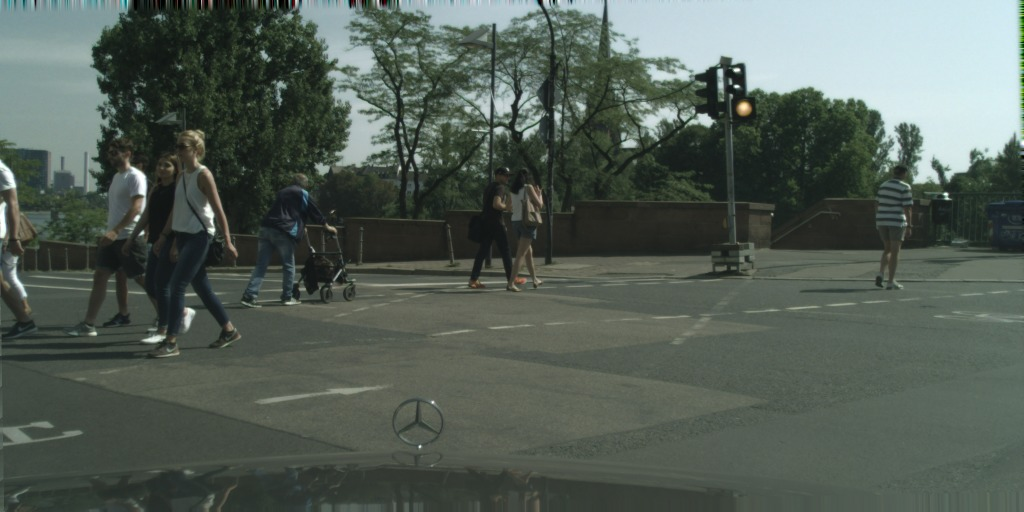
\includegraphics[width=0.48\textwidth,trim={0 20mm 0 0},clip]{segnet_114_output_0.jpg}
        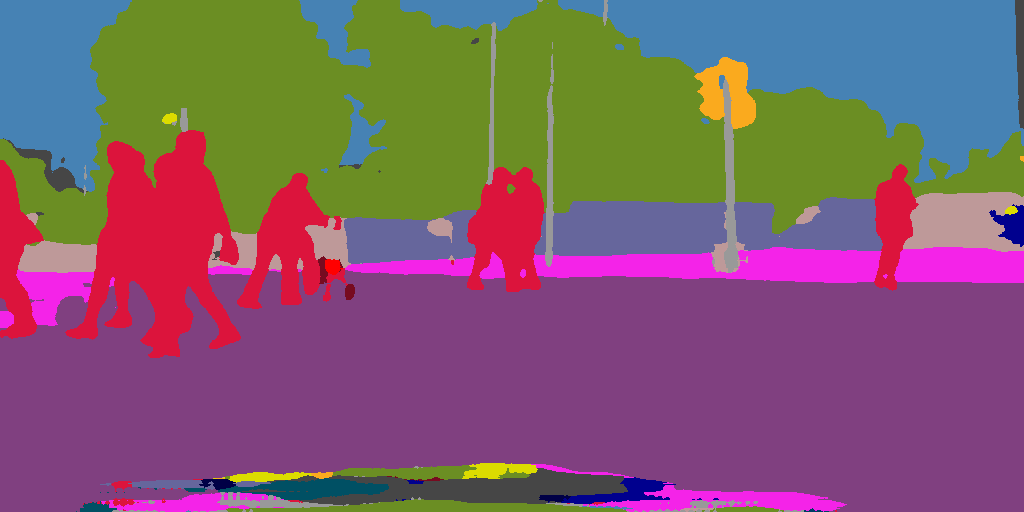
\includegraphics[width=0.48\textwidth,trim={0 20mm 0 0},clip]{segnet_114_output_1.png} \\
        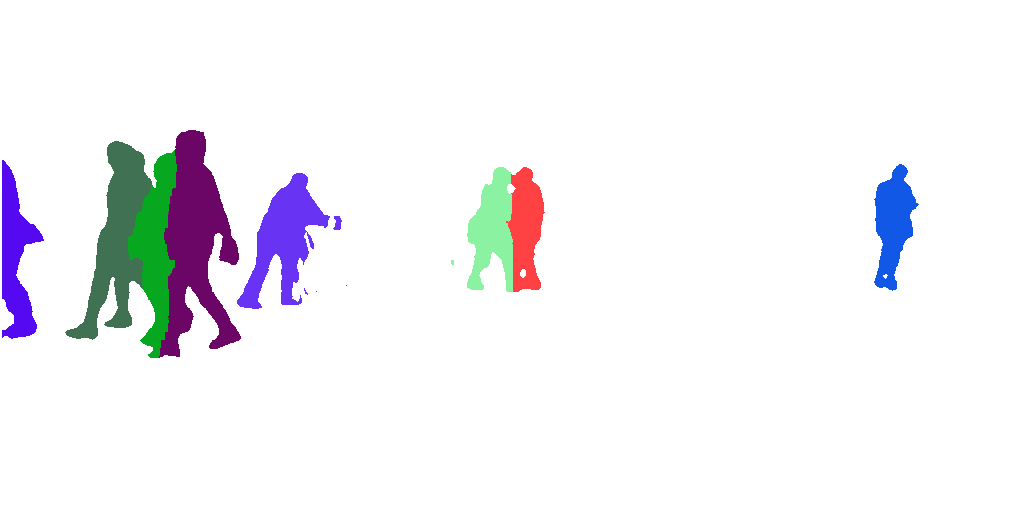
\includegraphics[width=0.48\textwidth,trim={0 20mm 0 0},clip]{segnet_114_output_3.png}
        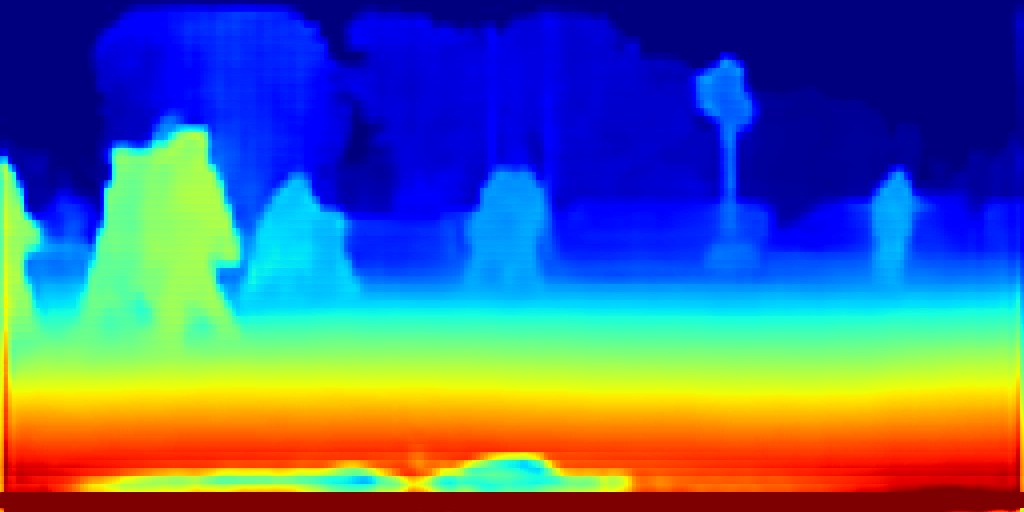
\includegraphics[width=0.48\textwidth,trim={0 20mm 0 0},clip]{segnet_114_output_4.png}
        \caption{Scene Understanding --- understanding the geometry and semantics of a scene. Clockwise from top-left: input image, semantic segmentation, depth prediction, instance segmentation.}
    \end{subfigure}
    \quad
    \begin{subfigure}[b]{0.3\textwidth}
\centering
        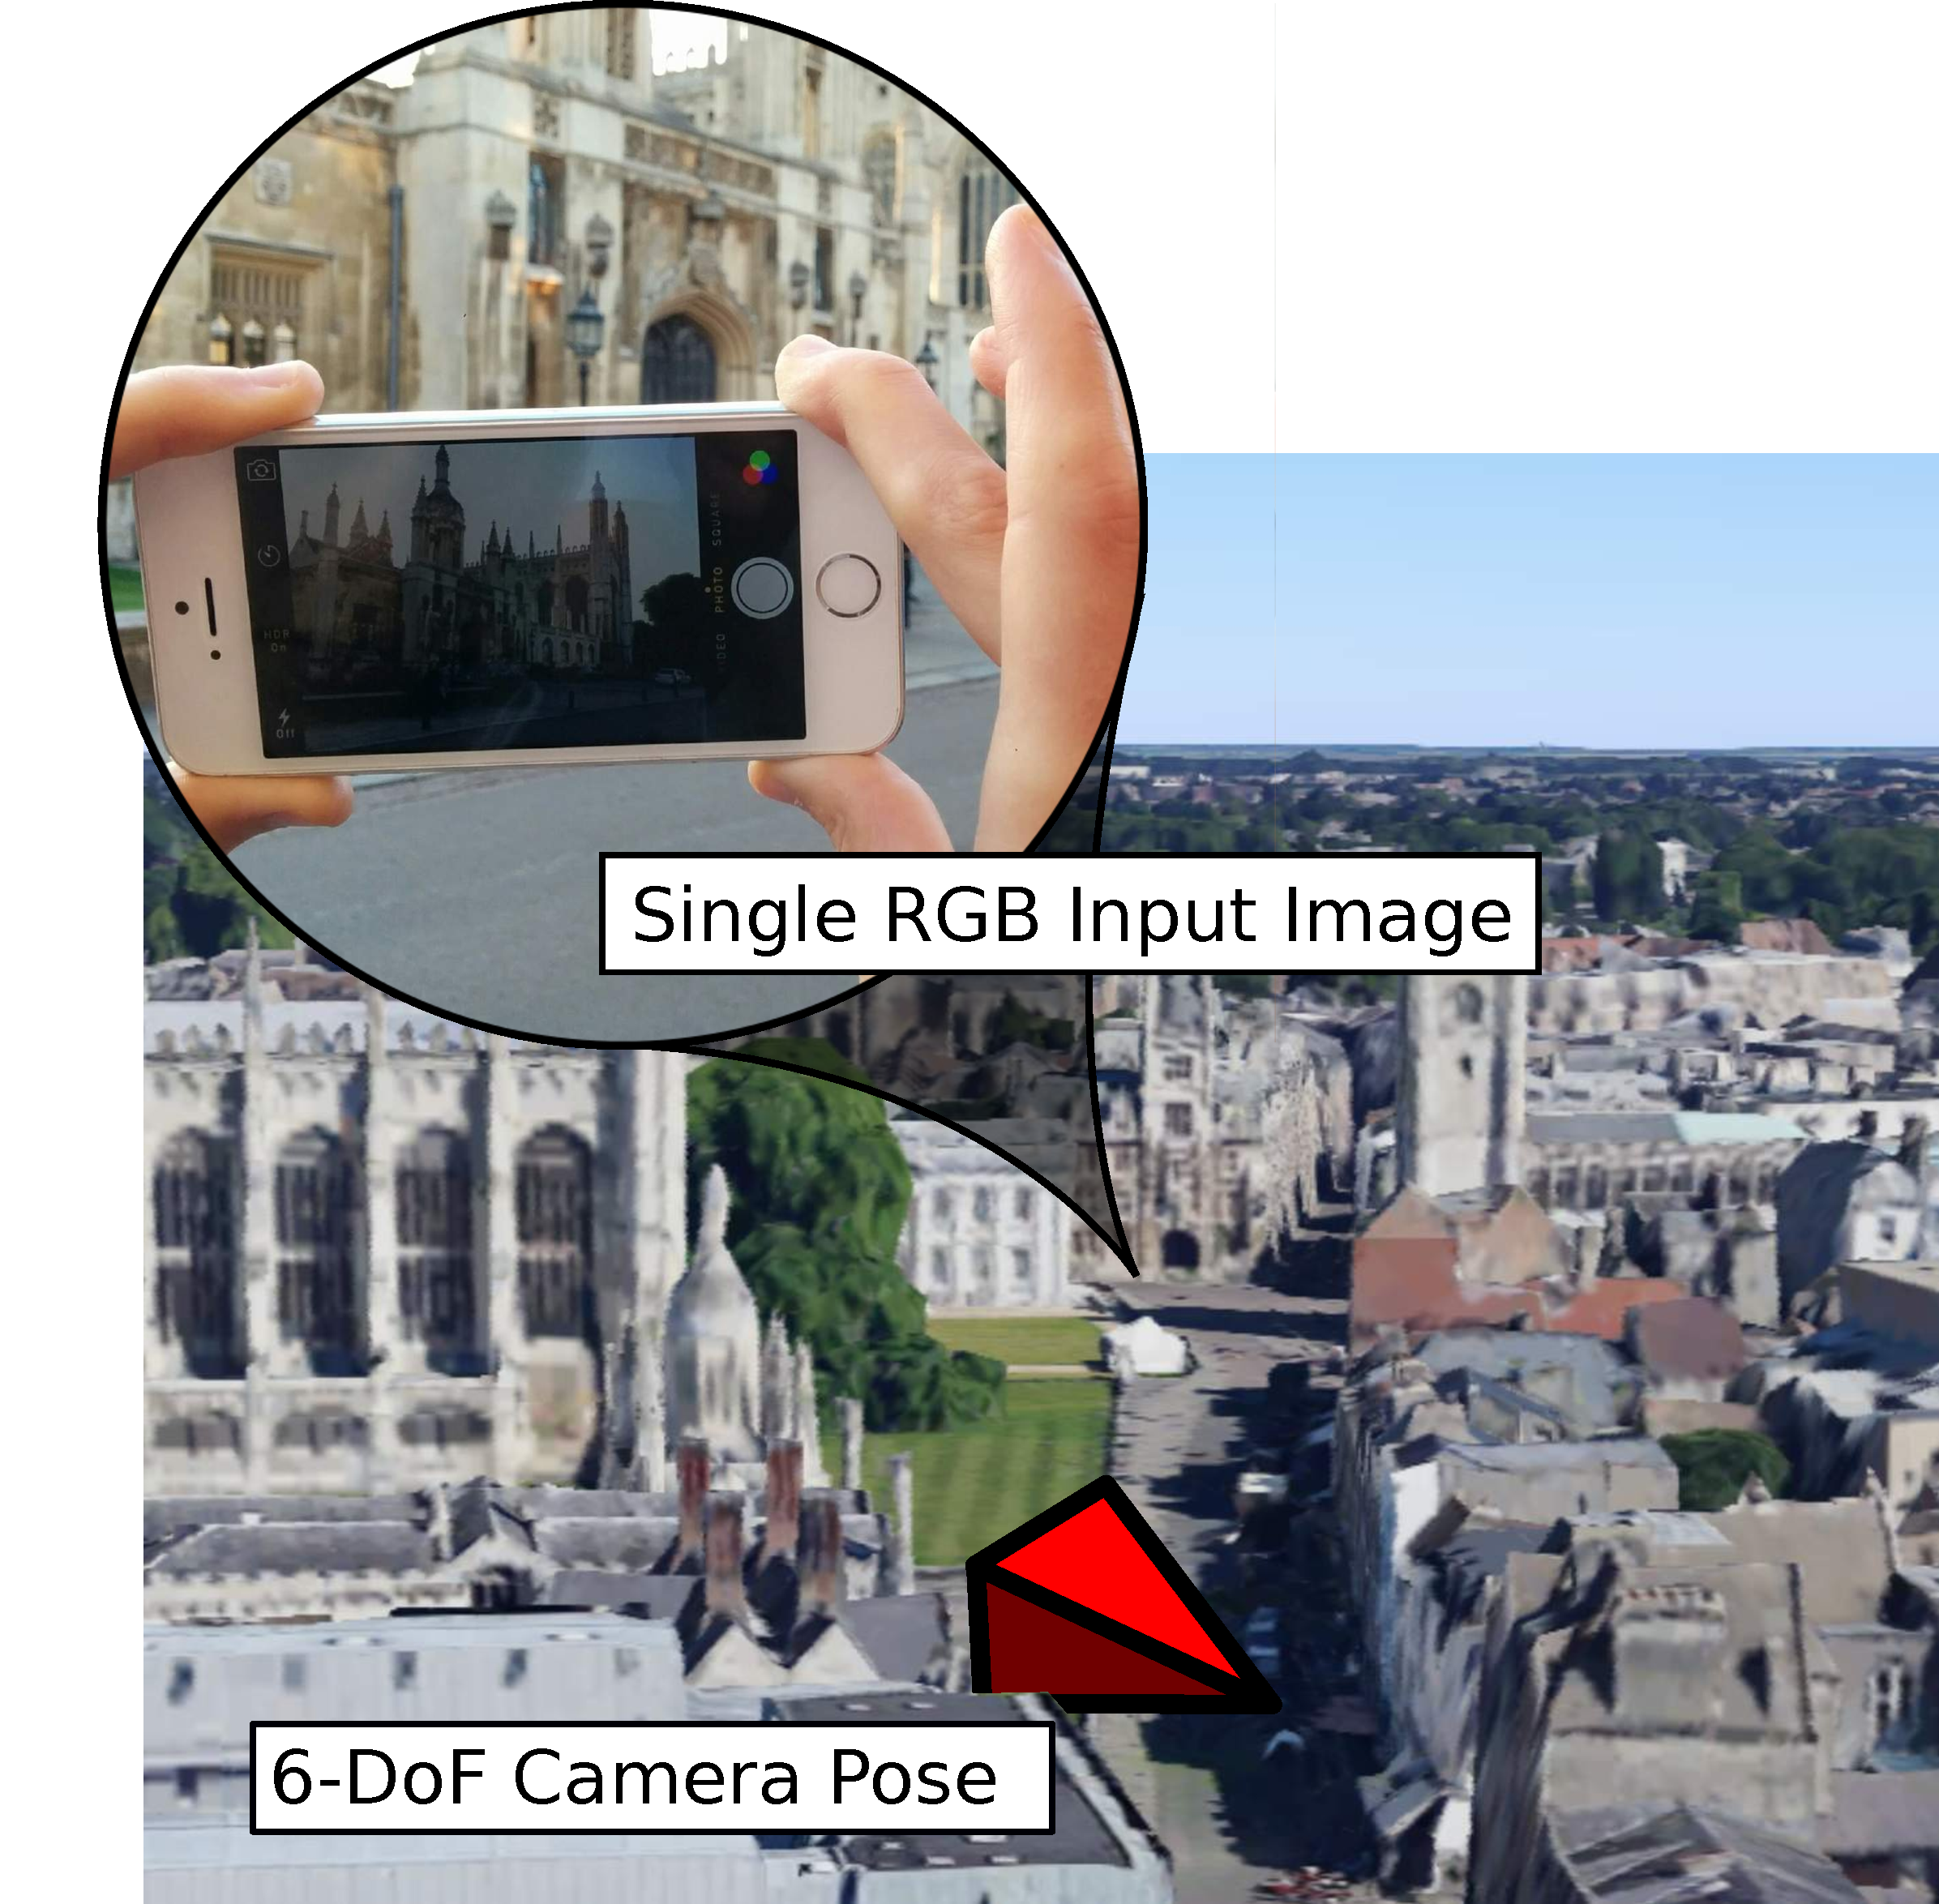
\includegraphics[width=\textwidth]{teaser.pdf}
        \caption{Localisation --- estimating the camera's 3D position and orientation from an image.}
    \end{subfigure}
    
    
    \begin{subfigure}[b]{\textwidth}
\centering
        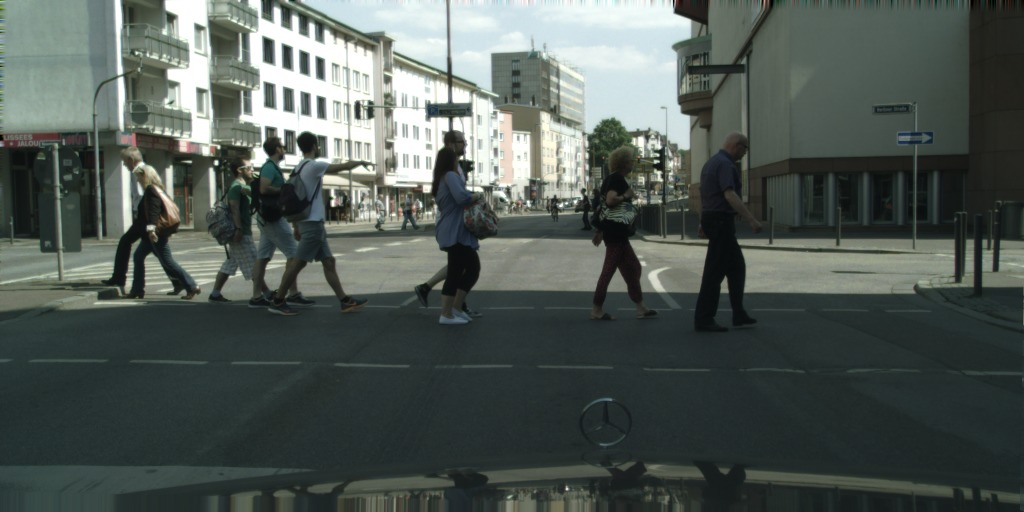
\includegraphics[width=0.32\textwidth,trim={0 20mm 0 0},clip]{Chapter2/Figs/results/segnet_107_output_0.jpg}
        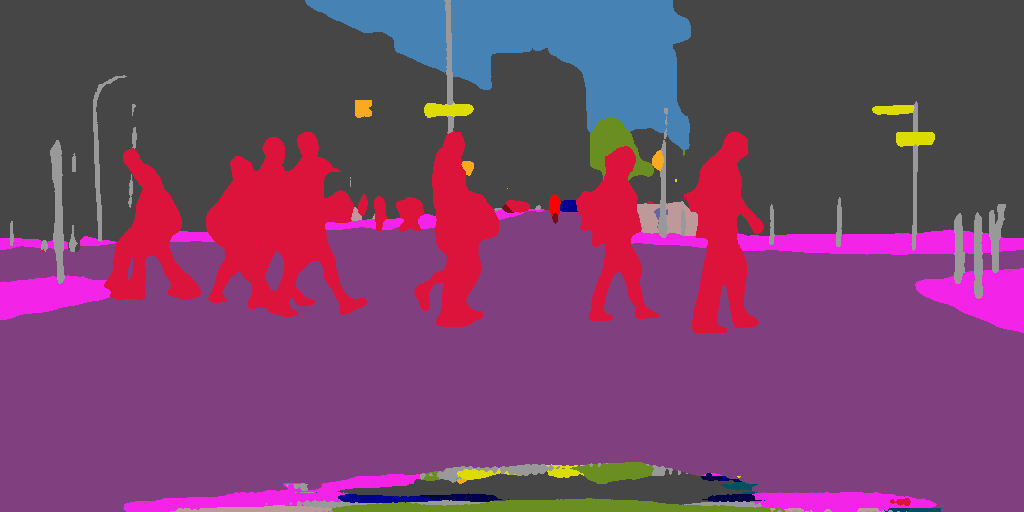
\includegraphics[width=0.32\textwidth,trim={0 20mm 0 0},clip]{Chapter2/Figs/results/segnet_107_output_1.png}
        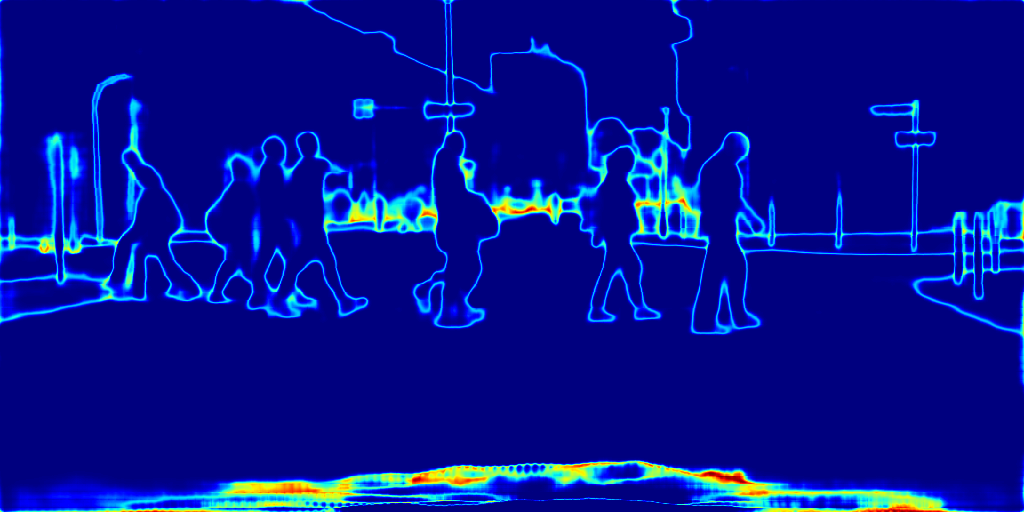
\includegraphics[width=0.32\textwidth,trim={0 20mm 0 0},clip]{Chapter2/Figs/results/segnet_107_output_2.png}
        \caption{Uncertainty --- understanding the prediction's confidence and what the model does not know. From left: input image, semantic segmentation, model uncertainty (where blue represents certain and more red colours are uncertain predictions). The model exhibits increased uncertainty in distance objects and around object boundaries.}
    \end{subfigure}
\caption[Examples of algorithms in this thesis.]{Examples of the variety of algorithms developed in this thesis. (a) shows a scene understanding system from \cref{scene_understanding}. (b) shows a localisation system which can determine the camera's 3D position and orientation in space from \cref{localisation}. (c) shows a semantic segmentation system which is aware of its uncertainty from \cref{scene_understanding}.}
\label{ch1:teaser}
\end{figure}

But end-to-end learning has problems too. It is often not good for data efficiency, interpretability or safety \citep{mcallister2017av_bdl}. This thesis makes two observations which challenge the weaknesses of end-to-end learning:
\begin{itemize}
\item We do not need to learn everything from scratch, we know many things about the world,
\item We cannot explain everything from our data and we need to know what our model does not know.
\end{itemize}
In this thesis, we focus on these ideas using concepts from \textbf{\textit{geometry}} and \textbf{\textit{uncertainty}}. These ideas are elaborated on in the next few sections.

\subsection{Machine Learning in Computer Vision}

Let us consider two arguments which motivate the use of machine learning approaches, in particular deep learning, to complicated computer vision problems.

First, as the most powerful demonstration of perception, how does the human visual pathway develop? Surprisingly, we are born without the ability to see \citep{gibson1960visual}. Infant humans learn through a mixture of semi-supervised and unsupervised learning \citep{kellman2006infant}. It typically takes three months to learn colour and depth perception. Object detection can take nine to twelve months. Suppose that an infant experiences one saccade (visual experience) per second of their first year of existence. This amounts to $1 \text{~saccade/s} \times 3600 \text{~sec/hour} \times 8 \text{~h/day} \times 365 \text{~days/year} = 10,000,000 \text{~training examples}$ in the first year of their life. Interestingly, this size is of the same order of magnitude as one of the largest computer vision datasets, ImageNet \citep{deng2009imagenet}. It is also the size of the data which is required for today’s image recognition models to achieve super-human performance \citep{he2016deep}. As our best example, the human visual system learns to see --- through nurture, not nature.

Secondly, it simply is not scalable to hand-design an algorithm
to support and adapt to complicated and dynamic data such as our visual world. Modern computer vision algorithms contain over 100 million parameters. Input data is very high dimensional, typically containing several million pixels being streamed over time. To date, we have been unable to specify hand-engineered rules to design top-performing architectures. To understand large amounts of data at scale we need to learn.

While there are many examples of machine learning models, \textit{deep convolutional neural networks} \citep{Fukushima1979neocognitron,krizhevsky2012imagenet} are most effective for vision tasks. Convolutional neural networks are a subset of deep learning which are particularly useful for computer vision because they are spatially invariant. Algorithms like stochastic gradient descent \citep{kiefer1952stochastic} and backpropagation \citep{rumelhart1986learning} can train networks containing millions of parameters. These networks can be optimised from a loss function formulated from supervised labelled training data or unsupervised learning.

Deep learning models have typically been restricted to classification settings. They excel at sub-sampling data and expanding feature dimensions to make classifications at an image level \citep{krizhevsky2012imagenet}. Applying these models to other problems in computer vision is more challenging. This is because other computer vision tasks require representations for recognition, registration or reconstruction \citep{cipolla2010computer}. Standard recognition encoder networks \citep{krizhevsky2012imagenet,simonyan2013deep,he2004multiscale} cannot be naively applied to these domains. This thesis proposes a broader range of deep learning architectures for many other computer vision problems.

Finally, there is an interesting comparison between deep learning models and the human visual system. The human visual cortex processes images from the retina initially through the V1-V4 and IT cortex \citep{hubel1962receptive}. Evidence shows that hierarchical representations are formed at increasing levels of abstraction (edges, lines, contours, objects, scenes) \citep{hubel1962receptive}. Similar levels of abstraction are seen with increasing convolutional neural network depth \citep{zeiler2014visualizing}.

\subsection{Geometry in Computer Vision}

Geometry is concerned with questions of shape, size, relative position of figures and the properties of space.
In computer vision, geometry is used to describe the structure and shape of the world. Specifically, it concerns measures such as depth, volume, shape, pose, disparity, motion or optical flow. We understand the mathematics of geometry very well \citep{koenderink1991solid,faugeras1993three,hartley2000}.
Consequently, there are a lot of complex relationships, such as depth and motion, which do not need to be learned from scratch with deep learning.
By building architectures which use this knowledge, we can simplify the learning problem.

The alternative paradigm to geometry is using semantic representations. 
Semantic representations use a language to describe relationships in the world. For example, we might describe an object as a `cat' or a `dog'.
Geometry has two attractive characteristics over semantics:
\begin{itemize}
\item Geometry can be directly observed. We see the world's geometry directly using vision.  At the most basic level, we can observe motion and depth directly from a video by following corresponding pixels between frames \citep{koenderink1991affine}.  Other interesting examples include observing shape from shading \citep{horn1989shape} or depth from stereo disparity \citep{scharstein2002taxonomy}. In contrast, semantic representations are often proprietary to a human language, with labels corresponding to a limited set of nouns, which cannot be directly observed from the world.
\item Geometry is based on continuous quantities. For example, we can measure depth in meters or disparity in pixels. In contrast, semantic representations are largely discretised quantities or binary labels.
\end{itemize}
With these properties, we show that we can use geometry to improve performance (\cref{localisation} and \cref{stereo}) and for unsupervised learning, without human-annotated labels (\cref{stereo} and \cref{motion}).

However, geometry alone cannot form a robust vision system. This is because models must learn representations which are robust to noise and outliers. Deep learning is powerful at learning representations which are robust to outliers and other nuisance variables. Additionally, models also need to be aware of the inherent uncertainty in the data.

\subsection{Uncertainty in Computer Vision}

Understanding what a model does not know is a critical part of many machine learning systems \citep{ghahramani2015probabilistic}. Uncertainty is important to improve trustworthiness and safety of these systems \citep{mcallister2017av_bdl}. Unfortunately, today's deep learning algorithms are usually unable to understand their uncertainty. These models are often taken blindly and assumed to be accurate, which is not always the case. For example, in two recent situations this has had disastrous consequences.

\begin{itemize}
\item In May 2016 the world tragically experienced the first fatality from an assisted driving system. According to the manufacturer's blog, `Neither Autopilot nor the driver noticed the white side of the tractor trailer against a brightly lit sky, so the brake was not applied' \citep{teslaCrashReport}.
\item In July 2015, an image classification system erroneously identified two African American humans as gorillas, raising concerns of racism and discrimination \citep{googleblackgorilla}.
\end{itemize}

If both these algorithms could assign a high level of uncertainty to their erroneous predictions, then each system may have been able to make better decisions and likely avoid disaster. Unfortunately, traditional machine learning approaches to understanding uncertainty, such as Gaussian processes \citep{rasmussen2006gaussian}, do not scale to high dimensional inputs like images and videos. 
To effectively understand this data, we need deep learning. But deep learning struggles to model uncertainty.

One of the techniques used in this thesis to model uncertainty is Bayesian deep learning \citep{mackay1992practical} which provides a deep learning framework which can model uncertainty.
Bayesian deep learning is a field at the intersection between deep learning and Bayesian probability theory.
It offers principled uncertainty estimates from deep learning architectures.
These deep architectures can model complex tasks by leveraging the hierarchical representation power of deep learning, while also being able to infer complex multi-modal posterior distributions.
Probabilistic deep learning models typically form uncertainty estimates by either placing distributions over model weights, or by learning a direct mapping to probabilistic outputs. In this thesis we show how to formulate accurate and scalable computer vision models which can understand the model's uncertainty with Bayesian deep learning.

\section{Contributions}

To summarise, the contributions of this thesis are as follows:
\begin{itemize}
\item We demonstrate how to formulate many challenging computer vision problems with end-to-end deep learning. We show the performance of these models significantly improves over traditional approaches.
\item We show how to improve performance of these models by leveraging the problem's geometry. We demonstrate that this reduces the amount of training data required and improves the generalisation of these models to novel examples.
\item Finally, for practical and safe systems, it is important to understand our model’s uncertainty. We show how to quantify uncertainty in deep learning computer vision models with Bayesian deep learning and probabilistic modelling.
\end{itemize}

\section{Co-Authored Papers}

Some extracts from this thesis appear in the following co-authored publications and preprints.
\cref{scene_understanding} contains work from:
\begin{itemize}
\item Vijay Badrinarayanan, Alex Kendall and Roberto Cipolla. SegNet: A Deep Convolutional Encoder-Decoder Architecture for Image Segmentation. IEEE Transactions on Pattern Analysis and Machine Intelligence, 2017.
\item Alex Kendall and Yarin Gal. What Uncertainties Do We Need in Bayesian Deep Learning for Computer Vision? Advances in Neural Information Processing Systems, 2017.
\item Alex Kendall, Yarin Gal and Roberto Cipolla. Multi-Task Learning Using Uncertainty to Weigh Losses for Scene Geometry and Semantics. Proceedings of the IEEE Conference on Computer Vision and Pattern Recognition, 2018.
\end{itemize}
\cref{localisation} is adapted from:
\begin{itemize}
\item Alex Kendall, Matthew Grimes and Roberto Cipolla. PoseNet: A Convolutional Network for Real-Time 6-DOF Camera Relocalization. Proceedings of the International Conference on Computer Vision, 2015.
\item Alex Kendall and Roberto Cipolla. Modelling Uncertainty in Deep Learning for Camera Relocalization. Proceedings of the International Conference on Robotics and Automation, 2016.
\item Alex Kendall and Roberto Cipolla. Geometric loss functions for camera pose regression with deep learning. Proceedings of the IEEE Conference on Computer Vision and Pattern Recognition, 2017.
\end{itemize}
\cref{stereo} extends:
\begin{itemize}
\item Alex Kendall, Hayk Martirosyan, Saumitro Dasgupta, Peter Henry, Ryan Kennedy, Abraham Bachrach, and Adam Bry. End-to-End Learning of Geometry and Context for Deep Stereo Regression. Proceedings of the International Conference on Computer Vision, 2017.
\end{itemize}
And finally, \cref{motion} is adapted from:
\begin{itemize}
\item Alex Kendall and Roberto Cipolla. Learning Semantics, Motion and Geometry for Video Scene Understanding. Under Review, 2017.
\end{itemize}

\section{Thesis Structure}

The outline of the thesis is as follows. The following four chapters discuss core computer vision tasks: scene understanding in \cref{scene_understanding}, localisation in \cref{localisation}, stereo vision in \cref{stereo}, video and motion in \cref{motion}. For each chapter’s topic, we review the prior art. We introduce formulations for end-to-end deep learning architectures. We discuss how to improve these end-to-end models with notions of the problem’s geometry. Finally, we show how to capture model uncertainty. In \cref{conclusions}, we make overall conclusions, discuss the application of this technology and suggest directions for future research.
%*******************************************************************************
%****************************** Second Chapter *********************************
%*******************************************************************************

% MATHS

\chapter{Scene Understanding}
\label{scene_understanding}

\graphicspath{{Chapter2/Figs/}}

\section{Introduction}

{\let\thefootnote\relax\footnote{{In this Chapter, \cref{segmentation} and \cref{segnet} was collaborative work with Vijay Badrinarayanan and Roberto Cipolla and was published in \citep{badrinarayanan2017segnet}. \cref{seg_unc} and \cref{sec:mlttask} was collaborative work with Yarin Gal and was published in \citep{kendall2017uncertainties} and \citep{kendall2017multi}, respectively.}}}

\begin{figure}[t]
\center
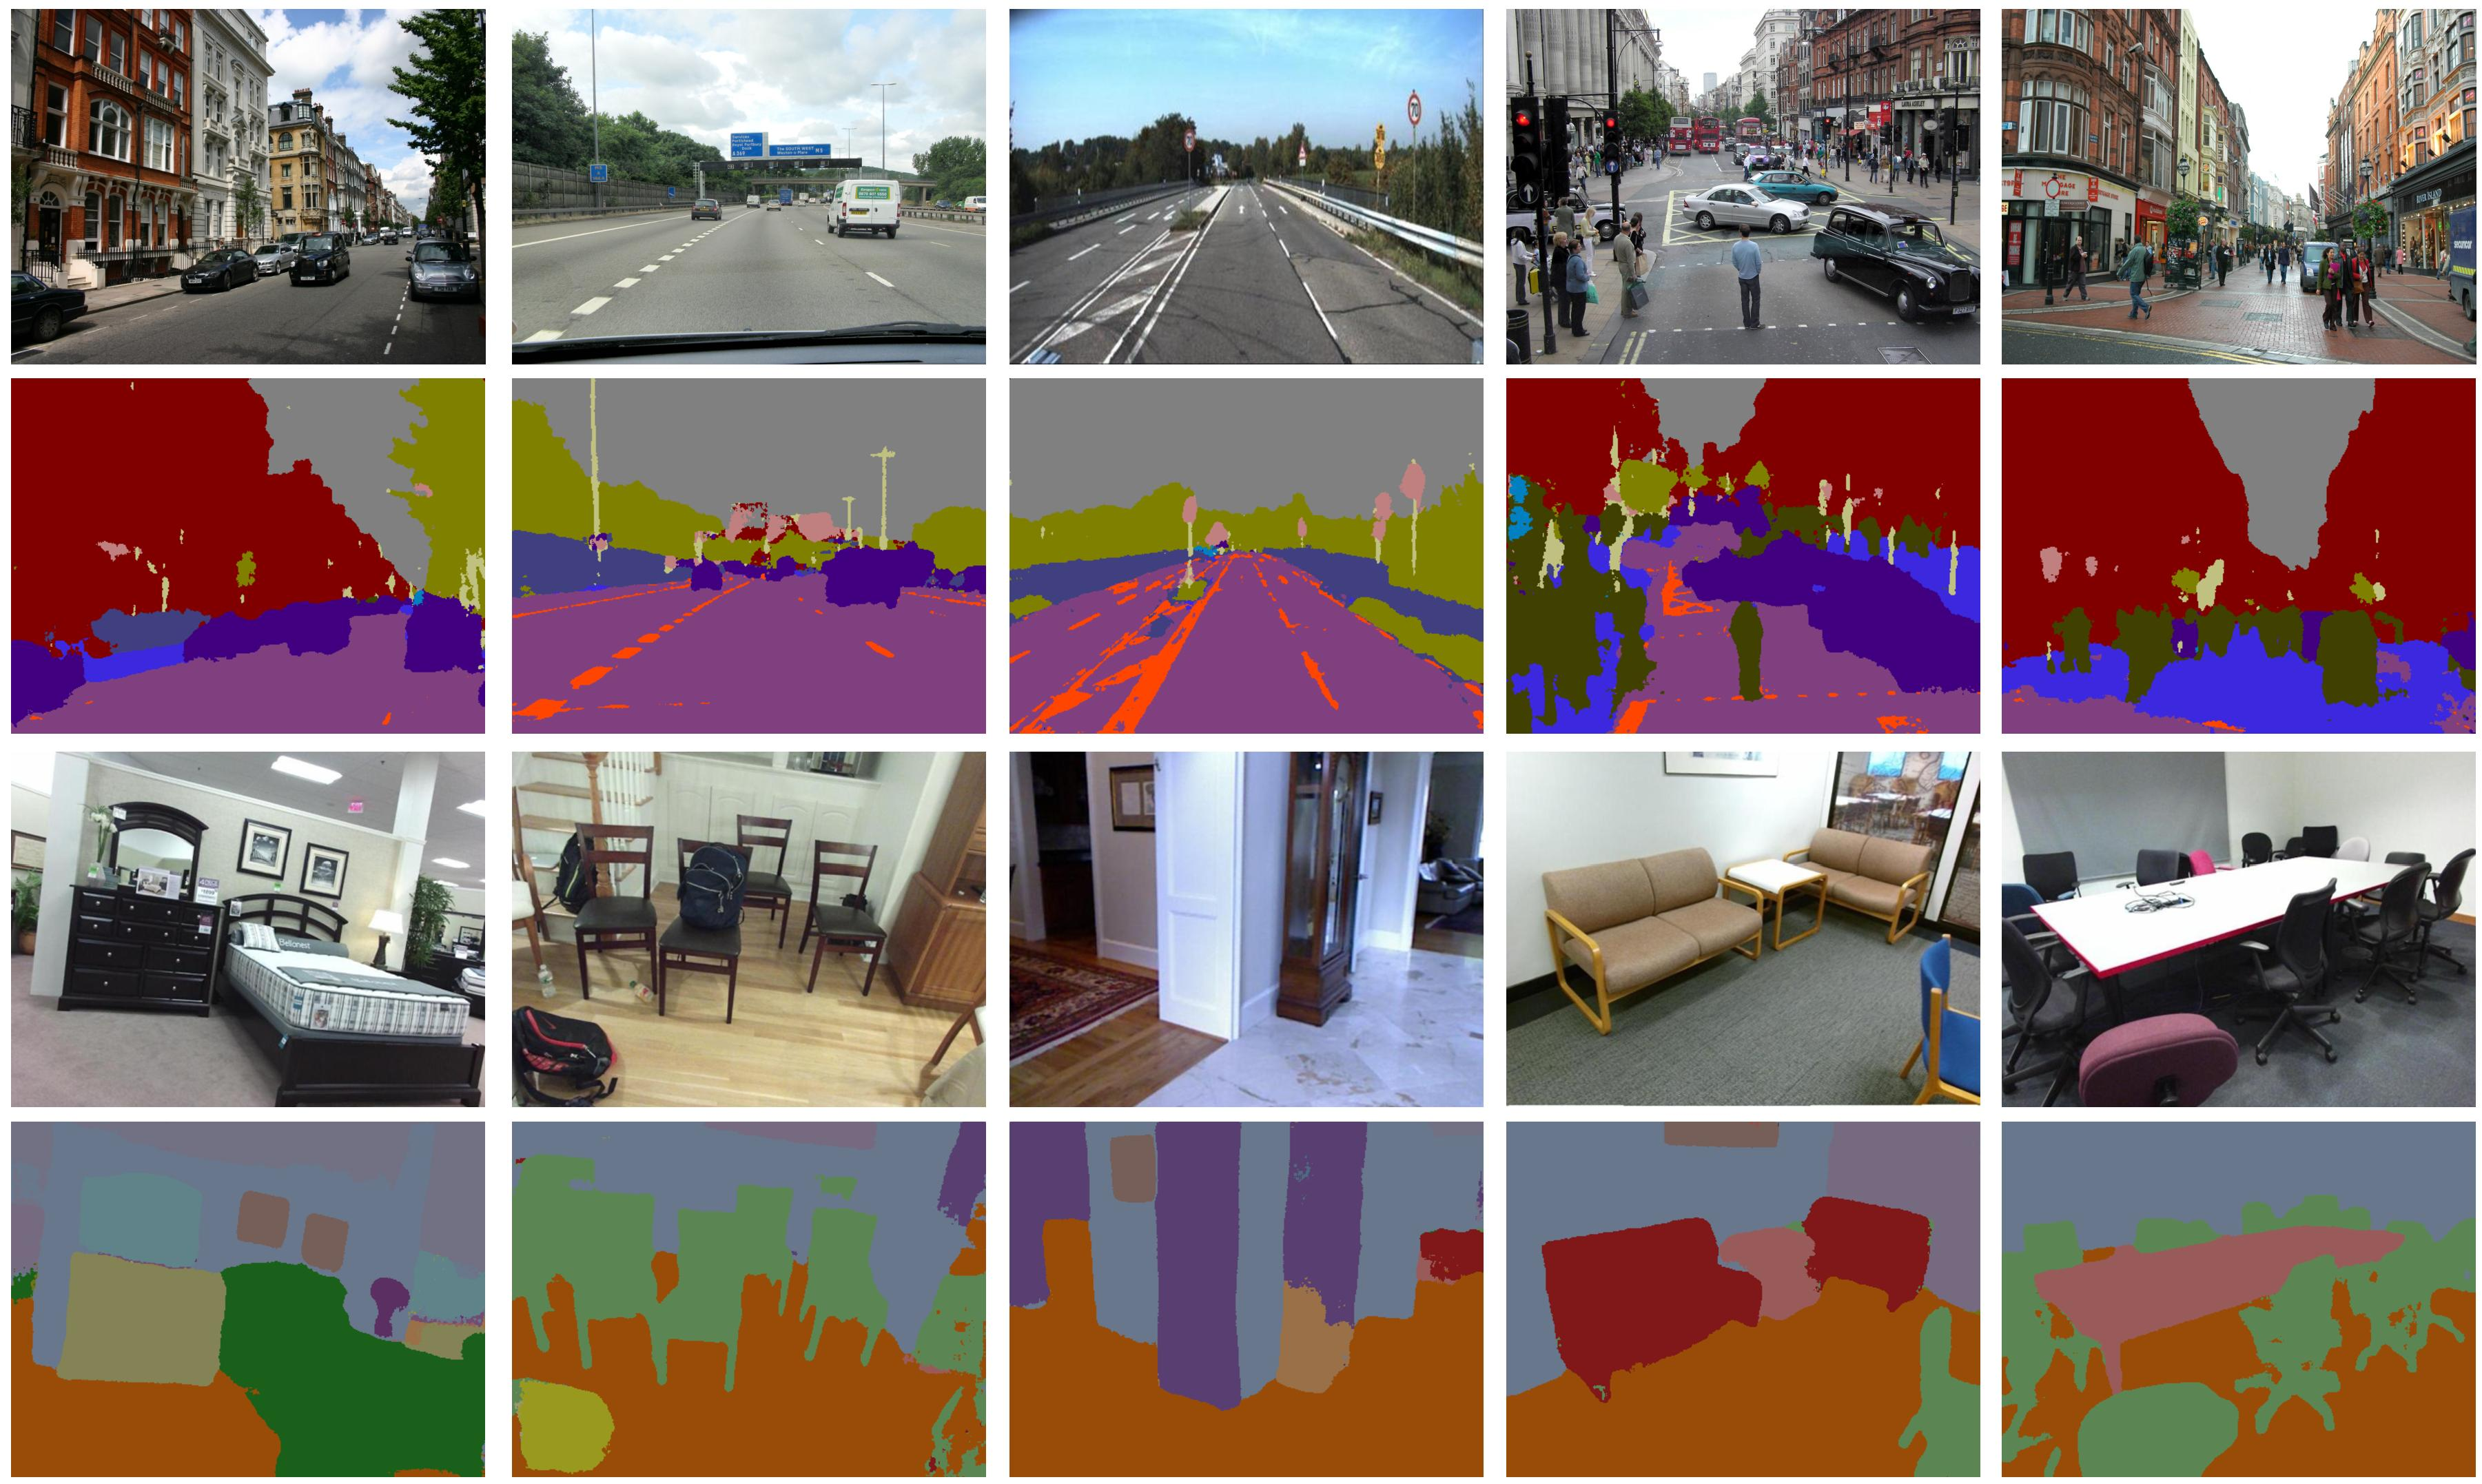
\includegraphics[width=\textwidth]{segnet/CamVidTeaserwithIndoorScenes.jpg}
\caption[SegNet semantic segmentation predictions on indoor and outdoor scenes.]{SegNet predictions on indoor and outdoor scene test samples from the wild. To try our system yourself, please see our online web demo at \url{http://mi.eng.cam.ac.uk/projects/segnet/}.}
\label{Teaser}
\end{figure}

In this chapter, we address the problem of scene understanding. Scene understanding is a task which is fundamental to computer vision. It requires extracting information about what is where \citep{marr1982vision}. Visual scene understanding algorithms must extract information about objects and their contextual relationships from the observed environment. Scene understanding requires knowledge of semantics and geometry and can be broken down into many subtasks. In this work we focus on the tasks of semantic segmentation, instance segmentation and depth prediction. Collectively, these three representations provide a fine-grained, per-pixel representation of objects and their geometry.

We begin the chapter by proposing a deep convolutional encoder-decoder architecture, SegNet, capable of learning per-pixel output. Motivated by the problem of semantic segmentation, we analyse different architectures for upsampling features and producing dense pixel-wise output. We benchmark the efficacy of SegNet on many datasets on road scene, indoor and object segmentation datasets. Some results are shown in \cref{Teaser}.

For practical systems, it is important to understand what our models do not know. In \cref{seg_unc}, we discuss two types of uncertainty; aleatoric and epistemic uncertainty \citep{der2009aleatory}. We derive deep learning models which can capture both forms of uncertainty using Bayesian deep learning \citep{mackay1992practical} and probabilistic modelling. We build models for semantic segmentation and per-pixel depth estimation with these ideas. We show modelling uncertainty gives an improvement in performance. We empirically evaluate the quality of these uncertainty metrics and their properties with respect to novel examples, with increasing distinction from the training dataset.

However, scene understanding requires joint knowledge of semantics and geometry. In \cref{sec:mlttask}, we present a framework for designing models capable of learning many tasks from a single representation, using multi-task learning. We make the observation that the relative weighting of each task's loss greatly influences performance. We derive a loss function which learns the task weights using probabilistic modelling. The final model jointly predicts semantic segmentation, instance segmentation and depth regression. Interestingly, we show that jointly learning these tasks in a single multi-task model out-performs equivalent models individually trained on each task.

\section{Semantic Segmentation}
\label{segmentation}

We begin by introducing the task of semantic segmentation, which is a core task in scene understanding. Semantic pixel-wise segmentation requires an estimate of each pixel's semantic class (see \cref{Teaser}).
It is an active topic of research, fuelled by challenging datasets \citep{brostow2009semantic,silberman2012indoor,Geiger2012CVPR,pascal,song2015sun,Cordts2016Cityscapes}. Before the arrival of deep learning, the best performing methods mostly relied on hand engineered features classifying pixels independently. Typically, an image patch was fed into a classifier, \textit{e.g.} random forests \citep{Jamie2,brostow2008segmentation} or boosting \citep{Sturgess,LadickyECCV}, to predict the class probabilities of the centre pixel. Features based on appearance \citep{Jamie2} or motion and appearance \citep{brostow2008segmentation,Sturgess, LadickyECCV} have been explored. These per-pixel noisy predictions (often called \textit{unary} terms) from the classifiers are then smoothed by using pair-wise (or higher order) conditional random fields (CRFs) \citep{Sturgess,LadickyECCV} to improve the accuracy. More recent approaches have aimed to produce high quality unaries by trying to predict the labels for all the pixels in a patch as opposed to only the centre pixel. This improves the results of random forest based unaries \citep{kontschieder2011structured}, but reduces performance on thin structures. Dense depth maps have also been used as input for classification using Random Forests \citep{zhang2010semantic}. Another approach argues for the use of a combination of popular hand designed features and spatio temporal super-pixels to obtain higher accuracy \citep{tighe2013superparsing}.

Indoor RGB-D pixel-wise semantic segmentation has also gained popularity since the release of the NYU dataset \citep{silberman2012indoor} which contains labelled RGB-D data collected from a Kinect sensor. Many papers demonstrate that inputting depth modality significantly improves segmentation performance \citep{ren2012rgb,silberman2012indoor,Hermans14ICRA,gupta2013perceptual}. However, all these methods use hand-engineered features for classifying RGB-D images. 

The success of deep convolutional neural networks for object classification has more recently led to researchers to exploit their feature learning capabilities for structured prediction problems such as segmentation. There have also been attempts to apply networks designed for object categorization to segmentation, particularly by replicating the deepest layer features in blocks to match image dimensions \citep{FarabetPAMI,FarabetPurityCover,Grangier,Gatta}. However, the resulting classification is coarse \citep{Grangier}. Another approach using recurrent neural networks \citep{pinheiro2014recurrent} merges several low resolution predictions to create input image resolution predictions. These techniques are already an improvement over hand engineered features \citep{FarabetPAMI} but their ability to delineate boundaries is poor. 

Newer deep architectures \citep{long2015fully,NohDeconvNets,eigen2015predicting,DecoupledNet,CRFRNN} particularly designed for segmentation have advanced the state-of-the-art by learning to decode or map low resolution image representations to pixel-wise predictions. These methods rely on pre-trained features from the large ImageNet object classification dataset \citep{deng2009imagenet}. For example, Fully Convolutional Networks (FCN) \citep{long2015fully} learn to up-sample its input feature map(s) and combines them with the corresponding encoder feature map to produce a dense output. It has a large number of trainable parameters in the encoder network (134M) but a very small decoder network (0.5M). The overall large size of this network makes it hard to train end-to-end on a relevant task. Therefore, the authors use a stage-wise training process. Each decoder in the decoder network is progressively added to an existing trained network. The network is grown until no further increase in performance is observed. 

The approach in FCN forms the \textit{core segmentation engine} for a number of other approaches \citep{ParseNetRabinovich,UrtasunSegmentation,CRFRNN,chen2016deeplab}. These methods append CRFs as a post-processing method to clean the segmentation. These methods are slow as they require either MAP inference over a CRF \citep{lin2015efficient}, \citep{UrtasunSegmentation} or aids such as region proposals \citep{NohDeconvNets} for inference. We believe the perceived performance increase obtained by using a CRF is due to the lack of good decoding techniques in their core feed-forward segmentation engine. 

Multi-scale deep architectures are also being pursued \citep{eigen2015predicting,lin2015efficient,hariharan2015hypercolumns,ParseNetRabinovich}. The common idea is to use features extracted at multiple scales to provide both local and global context \citep{mostajabi2014feedforward}. Feature maps from the early encoding layers retain more high frequency detail leading to sharper class boundaries. Some of these architectures are difficult to train due to their large parameter size \citep{eigen2015predicting}. Again, a multi-stage training process is employed along with data augmentation. Inference is also expensive with multiple convolutional pathways for feature extraction.

All of the latest state-of-the-art semantic segmentation models use supervised deep learning \citep{badrinarayanan2017segnet,long2015fully}, benefiting from residual architectures \citep{he2016deep,huang2017densely}. Recent work has focused on improving the receptive field of features and providing them with more context for semantic reasoning, for example using dilated convolutions \citep{YuKoltun2016} and pyramid spatial pooling \citep{zhao2017pspnet}. We have also seen semantic segmentation combined with other tasks, such as instance segmentation \citep{he2017maskrcnn} and geometry \citep{kendall2017multi} in multi-task learning settings.

In the next section, we introduce the SegNet architecture, which was one of the first end-to-end deep convolutional neural networks for semantic segmentation. We compare the different decoding techniques to form pixel-wise prediction with deep learning and benchmark our approach on a number of challenging datasets.

\section{SegNet Architecture}
\label{segnet}

\begin{figure*}[t]
\center
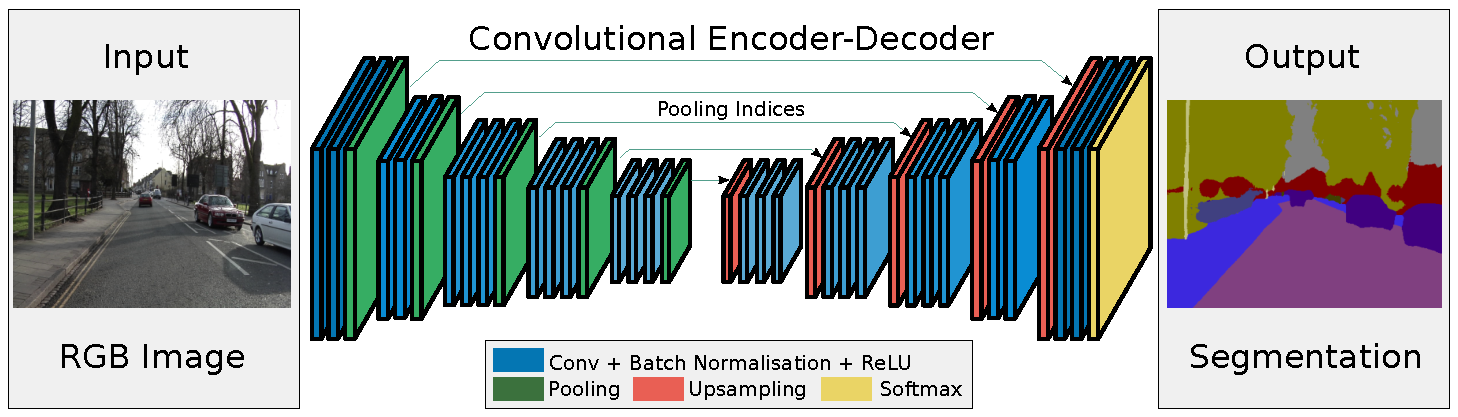
\includegraphics[width=0.95\textwidth]{segnet/segnet_softmax.pdf}
\caption[SegNet architecture.]{An illustration of the SegNet architecture. There are no fully connected layers and hence it is only convolutional. The decoder upsamples the encoded features using the corresponding pooling indices from the encoder to produce sparse feature maps. It then performs convolution with a trainable filter bank to densify the feature map. The final decoder output feature maps are fed to a softmax classifier for pixel-wise classification.}
\label{SegNetArchitecture}
\end{figure*}

The latest semantic segmentation architectures have tried to directly adopt deep architectures designed for category prediction to pixel-wise labelling \citep{long2015fully,FarabetPAMI}. The results, although very encouraging, appear coarse \citep{chen2016deeplab}. This is primarily because max-pooling and sub-sampling reduce feature map resolution in the encoder for recognition tasks. In this section, we design SegNet, a deep convolutional encoder-decoder architecture capable of outputting pixel-wise labels at full resolution. Our motivation to design SegNet arises from this need to map low resolution features to input resolution for pixel-wise classification. This mapping must produce features which are useful for accurate boundary localization. 

Our architecture, SegNet, is designed to be a \textit{core segmentation engine} for pixel-wise semantic segmentation. It is primarily motivated by road scene understanding applications which require the ability to model appearance (road, building), shape (cars, pedestrians) and understand the spatial-relationship (context) between different classes such as road and side-walk. In typical road scenes, the majority of the pixels belong to large classes such as road, building or sky and hence the network must produce smooth segmentations. The engine must also have the ability to delineate moving and other objects based on their shape despite their small size. Hence it is important to retain boundary information in the extracted image representation. From a computational perspective, it is necessary for the network to be efficient in terms of both memory and computation time during inference. It must also be able to train end-to-end in order to jointly optimise all the weights in the network using an efficient weight update technique such as stochastic gradient descent (SGD) \citep{Bottou}. Networks that are trained end-to-end or equivalently those that do not use multi-stage training \citep{long2015fully} or other supporting aids such as region proposals \citep{NohDeconvNets} help establish benchmarks that are more easily repeatable. The design of SegNet arose from a need to match these criteria.

SegNet has an encoder network and a corresponding decoder network, followed by a final pixel-wise classification layer. This architecture is illustrated in \cref{SegNetArchitecture}. The encoder network consists of $13$ convolutional layers which is topologically identical to the convolutional layers in VGG16 \citep{simonyan2014very}. We can therefore initialize the training process from weights trained for classification on large datasets \citep{deng2009imagenet}. We remove the fully connected layers of VGG16 which makes the SegNet encoder network significantly smaller (from $134$ million parameters to $14.7$ million) than many other recent architectures \citep{long2015fully,NohDeconvNets,ParseNetRabinovich,DecoupledNet}. 

The key component of SegNet is the decoder network which consists of a hierarchy of decoders one corresponding to each encoder. Of these, the appropriate decoders use the max-pooling indices received from the corresponding encoder to perform non-linear upsampling of their input feature maps. This idea was inspired from an architecture designed for unsupervised feature learning \citep{Ranzato}. Reusing max-pooling indices in the decoding process has several practical advantages; (i) it improves boundary delineation, (ii) it reduces the number of  parameters enabling end-to-end training, and (iii) this form of upsampling can be incorporated into any encoder-decoder architecture such as \citet{long2015fully} or \citet{CRFRNN} with slight modification. The final decoder output is fed to a multi-class softmax classifier to produce class probabilities for each pixel independently.

Each \textit{encoder} in the encoder network performs convolution with a filter bank to produce a set of feature maps. These are then batch normalized \citep{BN}). Then an element-wise rectified-linear non-linearity (ReLU) $max(0,x)$ is applied. Following that, max-pooling with a $2\times2$ window and stride $2$ (non-overlapping window) is performed and the resulting output is sub-sampled by a factor of $2$. Max-pooling is used to achieve translation invariance over small spatial shifts in the input image. Sub-sampling results in a large receptive field for each pixel in the feature map. However, sub-sampling reduces spatial resolution of the features which is not beneficial for segmentation where boundary delineation is vital. Therefore, it is necessary to \textit{capture and store} boundary information in the encoder feature maps before sub-sampling is performed. If memory during inference is not constrained, then all the encoder feature maps (after sub-sampling) can be stored. This is usually not the case in practical applications and hence we propose a more efficient way to store this information. It involves storing only the max-pooling \textit{indices}, i.e, the locations of the maximum feature value in each pooling window is memorized for each encoder feature map. In principle, this can be done using 2 bits for each $2\times2$ pooling window and is thus much more efficient to store as compared to memorizing feature map(s) in float precision (such as U-Net \citep{ronneberger2015u}). As we show later in this work, this lower memory storage results in a slight loss of accuracy but is still suitable for practical applications.

The appropriate \textit{decoder} in the decoder network upsamples its input feature map(s) using the memorized max-pooling indices from the corresponding encoder feature map(s). This step produces sparse feature map(s). This SegNet decoding technique is illustrated in \cref{Upsampling}. These feature maps are then convolved with a trainable decoder filter bank to produce dense feature maps. A batch normalization step is then applied to each of these maps. Note that the decoder corresponding to the first encoder (closest to the input image) produces a multi-channel feature map, although its encoder input has 3 channels (RGB). This is unlike the other decoders in the network which produce feature maps with the same number of size and channels as their encoder inputs. The high dimensional feature representation at the output of the final decoder is fed to a trainable soft-max classifier. This soft-max classifies each pixel independently. The output of the soft-max classifier is a K channel image of probabilities where K is the number of classes. The predicted segmentation corresponds to the class with maximum probability at each pixel.

In the following Sections, we evaluate the performance of SegNet on a number of datasets \citep{pascal,hariharan2011semantic} and scene understanding challenges such as CamVid road scene segmentation \citep{brostow2009semantic}. We analyse different decoding techniques and the practical trade-offs when designing segmentation architecture. In addition, we present a real-time online demo of road scene segmentation into 11 classes of interest for autonomous driving (see \cref{Teaser}). Some example test results produced on randomly sampled road scene images from the internet are shown in \cref{Teaser}.

\begin{figure*}
\centering
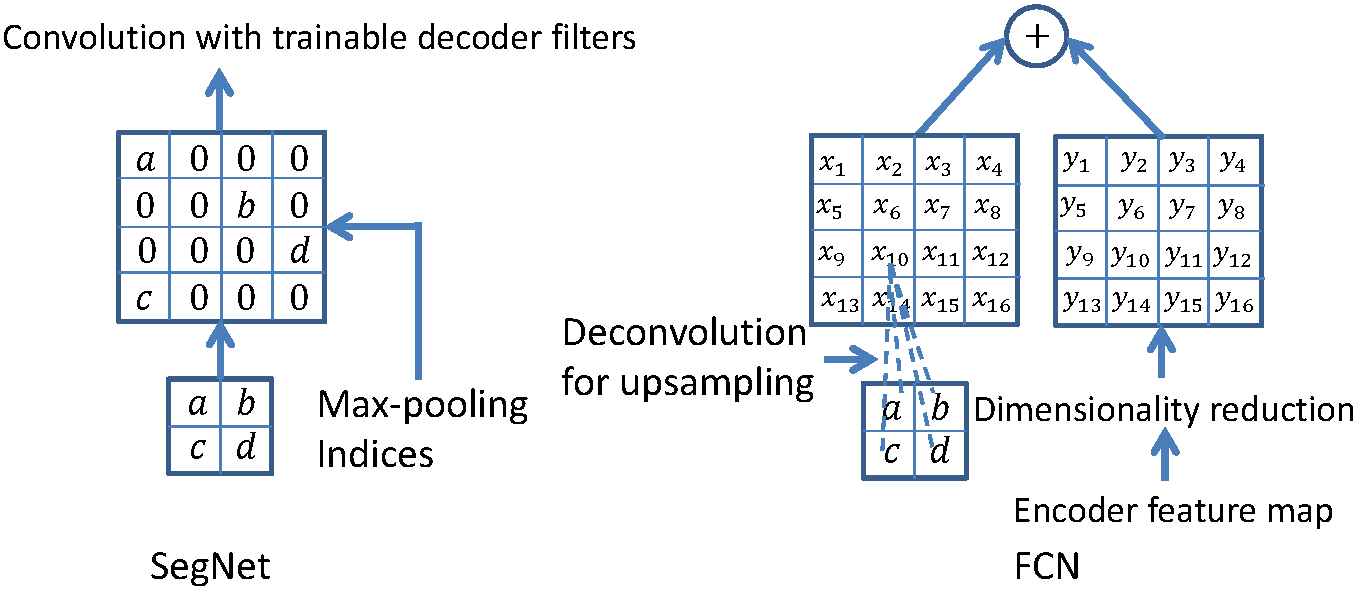
\includegraphics[width=\textwidth]{segnet/decoderVariantsNew.pdf}
\caption[SegNet decoder.]{An illustration of SegNet and FCN \citep{long2015fully} decoders. $a,b,c,d$ correspond to values in a feature map. SegNet uses the max pooling indices to upsample (without learning) the feature map(s) and convolves with a trainable decoder filter bank. FCN upsamples by learning to deconvolve the input feature map and adds the corresponding encoder feature map to produce the decoder output. This feature map is the output of the max-pooling layer (includes sub-sampling) in the corresponding encoder. Note that there are no trainable decoder filters in FCN.}
\label{Upsampling}
\end{figure*}

\subsection{Decoder Variants}
\label{Variants}

One of the main contributions of this Section is our analysis of decoding techniques for semantic segmentation. Most recent deep architectures for segmentation have identical encoder networks, \textit{i.e.} VGG16 \citep{simonyan2014very} or ResNet101 \citep{he2016deep}, but differ in the form of the decoder network, training and inference. Another common feature is they have trainable parameters in the order of hundreds of millions and thus encounter difficulties in performing end-to-end training \citep{NohDeconvNets}. The difficulty of training these networks has led to multi-stage training \citep{long2015fully}, appending networks to a pre-trained core segmentation engine such as FCN \citep{CRFRNN}, use of supporting aids such as region proposals for inference \citep{NohDeconvNets}, disjoint training of classification and segmentation networks \citep{DecoupledNet} and use of additional training data for pre-training \citep{ParseNetRabinovich} \citep{mottaghi2014role} or for full training \citep{CRFRNN}. In addition, performance boosting post-processing techniques \citep{chen2016deeplab} have also been popular. Although all these factors improve performance on challenging benchmarks \citep{pascal}, it is unfortunately difficult from their quantitative results to disentangle the key design factors necessary to achieve good performance. We therefore analyse many segmentation decoders in a controlled setting.

In order to analyse SegNet and compare its performance with other decoder variants we use a smaller version of SegNet, termed \textbf{SegNet-Basic}, which has 4 encoders and 4 decoders. All the encoders in SegNet-Basic perform max-pooling and sub-sampling and the corresponding decoders upsample its input using the received max-pooling indices. Batch normalization is used after each convolutional layer in both the encoder and decoder network. No biases are used after convolutions and no ReLU non-linearity is present in the decoder network. Further, a constant kernel size of $7\times7$ over all the encoder and decoder layers is chosen to provide a wide context for smooth labelling \textit{i.e.} a pixel in the deepest layer feature map (layer $4$) can be traced back to a context window in the input image of $106\times106$ pixels. This small size of SegNet-Basic allows us to explore many different variants (decoders) and train them in reasonable time. Similarly we create \textbf{FCN-Basic}, a comparable version of FCN for our analysis which shares the same encoder network as SegNet-Basic but with the FCN decoding technique in the corresponding decoders.  

On the left in \cref{Upsampling} is the decoding technique used by SegNet (also SegNet-Basic), where there is no learning involved in the upsampling step. However, the upsampled maps are convolved with trainable multi-channel decoder filters to densify the sparse inputs. Each decoder filter has the same number of channels as the number of upsampled feature maps. A smaller variant is one where the decoder filters are single channel, i.e they only convolve their corresponding upsampled feature map. This variant (\textbf{SegNet-Basic-SingleChannelDecoder}) reduces the number of trainable parameters and inference time significantly.

On the right in \cref{Upsampling} is the FCN (also FCN-Basic) decoding technique \citep{long2015fully}. The important design element of the FCN model is the dimensionality reduction step of the encoder feature maps. This \textit{compresses} the encoder feature maps which are then used in the corresponding decoders. Dimensionality reduction of the encoder feature maps, say of 64 channels, is performed by convolving them with $1\times 1\times 64\times K$ trainable filters, where $K$ is the number of classes. The compressed $K$ channel final encoder layer feature maps are the input to the decoder network. In a decoder of this network, upsampling is performed by convolution using a trainable \textit{multi-channel upsampling kernel}. We set the kernel size to $8\times8$. This manner of upsampling is also termed as \textit{sub-pixel convolution}, \textit{deconvolution} or \textit{transposed convolution}. Note that in SegNet the multi-channel convolution using trainable decoder filters is performed after upsampling to densifying feature maps. The upsampled feature map in FCN is then added to the corresponding resolution encoder feature map to produce the output decoder feature map. The upsampling kernels are initialized using bilinear interpolation weights \citep{long2015fully}. 

The FCN decoder model requires storing encoder feature maps during inference. This can be memory intensive, for e.g. storing 64 feature maps of the first layer of FCN-Basic at $180\times240$ resolution in 32 bit floating point precision takes 11MB. This can be made smaller using dimensionality reduction to the 11 feature maps which requires $\approx$ 1.9MB storage. SegNet on the other hand requires almost negligible storage cost for the pooling indices ($0.17$MB if stored using 2 bits per $2\times2$ pooling window). We can also create a variant of the FCN-Basic model which discards the encoder feature map addition step and only learns the upsampling kernels (\textbf{FCN-Basic-NoAddition}). 

In addition to the above variants, we study upsampling using fixed bilinear interpolation weights which therefore requires no learning for upsampling (\textbf{Bilinear-Interpolation}). At the other extreme, we can add 64 encoder feature maps at each layer to the corresponding output feature maps from the SegNet decoder to create a more memory intensive variant of SegNet (\textbf{SegNet-Basic-EncoderAddition}). Another and more memory intensive FCN-Basic variant (\textbf{FCN-Basic-NoDimReduction}) is where there is no dimensionality reduction performed for the encoder feature maps. Finally, please note that to encourage reproduction of our results we release the Caffe \citep{jia2014caffe} implementation of all the variants\footnote{See \url{http://mi.eng.cam.ac.uk/projects/segnet/} for our SegNet code and web demo.}. 

We also tried other generic variants where feature maps are simply upsampled by \textit{replication} \citep{FarabetPAMI}, or by using a fixed (and sparse) array of indices for upsampling. These performed quite poorly in comparison to the above variants. A variant without max-pooling and sub-sampling in the encoder network (decoders are redundant) consumes more memory, takes longer to converge and performs poorly. 

\subsection{Training}
\label{Training}


\afterpage{%
    \clearpage% Flush earlier floats (otherwise order might not be correct)
    \begin{landscape}% Landscape page
\begin{table*}[t]
\centering
\resizebox{\linewidth}{!}{
\begin{tabular}{c|c|c|c|ccc|ccc}
%\hline
\multicolumn{4}{c}{} &  \multicolumn{3}{c}{Median frequency balancing} & \multicolumn{3}{|c}{Natural frequency balancing} \\
\hline
& & Encoder & Infer & \multicolumn{3}{c|}{} &  \multicolumn{3}{c}{}\\
Variant &Params (M) &  storage (MB) &  time (ms) & G & C & IoU & G & C & IoU \\ \hline \hline
\multicolumn{10}{c}{Fixed upsampling} \\ \hline
Bilinear-Interpolation & 0.625 & 0 & 24.2 & 77.9 & 61.1 & 43.3 & 82.7 & 52.5 & 43.8 \\ \hline
\multicolumn{10}{c}{Upsampling using max-pooling indices} \\ \hline
SegNet-Basic & 1.425 & 1x & 52.6 & 82.7 & 62.0 & 47.7 & 84.0 & 54.6 & 46.3 \\ \hline
SegNet-Basic-EncoderAddition &1.425 & 64x & 53.0 & 83.4 & \textbf{63.6} & 48.5 & \textbf{84.2} & 56.5 & \textbf{47.7} \\ \hline
SegNet-Basic-SingleChannelDecoder& 0.625 &  1x & 33.1 &  81.2 & 60.7 & 46.1 & 83.5 & 53.9 & 45.2 \\ \hline
\multicolumn{10}{c}{Learning to upsample (bilinear initialisation)} \\ \hline
FCN-Basic & 0.65 & 11x & 24.2  & 81.7 & 62.4 & 47.3 &  83.9 & 55.6 & 45.0 \\ \hline
FCN-Basic-NoAddition &0.65 & n/a & 23.8 & 80.5 & 58.6 & 44.1 & 82.3 & 53.9 & 44.2 \\ \hline
FCN-Basic-NoDimReduction &1.625 & 64x & 44.8 & \textbf{84.1} & 63.4 & \textbf{50.1} & 83.5 & \textbf{57.3} & 47.0 
\\ \hline
FCN-Basic-NoAddition-NoDimReduction &1.625 & 0 & 43.9 & 80.5 & 61.6 & 45.9 & 83.7 & 54.8 & 45.5 \\ \hline 
\end{tabular}}

\caption[Quantitative segmentation decoder comparison.]{Comparison of decoder variants on the CamVid dataset. We quantify the performance using global (G), class average (C) and mean of intersection over union (IoU) metrics. The testing accuracies are shown as percentages for both natural frequency and median frequency balanced training loss function. SegNet-Basic performs at the same level as FCN-Basic but requires only storing max-pooling indices and is therefore more memory efficient during inference. Note that the theoretical memory requirement reported is based only on the size of the first layer encoder feature map. Networks with larger decoders and those using the encoder feature maps in full perform best, although they are least efficient.}
\label{PoolingQuantCAFFE}
\end{table*}
\end{landscape}}

We use the CamVid road scenes dataset \citep{brostow2009semantic} to benchmark the performance of the decoder variants. This dataset is small, consisting of 367 training and 233 testing RGB images (day and dusk scenes) at $360\times480$ resolution. The challenge is to segment $11$ classes such as road, building, cars, pedestrians, signs, poles, side-walk \textit{etc}. We perform local contrast normalization \citep{Jarrett} to the RGB input.

The encoder and decoder weights were all initialized using the technique described in He \emph{et~al.} \citep{he2015delving}. To train all the variants we use stochastic gradient descent (SGD) with a fixed learning rate of 0.1 and momentum of 0.9 \citep{Bottou} using our Caffe implementation of SegNet-Basic \citep{jia2014caffe}. We train the variants until the training loss converges. Before each epoch, the training set is shuffled and each mini-batch (12 images) is then picked in order thus ensuring that each image is used only once in an epoch. We select the model which performs highest on a validation dataset.

We use the cross-entropy loss \citep{long2015fully} as the objective function for training the network. The loss is averaged up over all the pixels in a mini-batch which contain a valid label. When there is large variation in the number of pixels in each class in the training set (e.g road, sky and building pixels dominate the CamVid dataset) then there is a need to weight the loss differently based on the true class. This is termed \textit{class balancing}. We use \textit{median frequency balancing} where the weight assigned to a class in the loss function is the ratio of the median of class frequencies computed on the entire training set divided by the class frequency. Therefore, we weight each pixel's loss by
\begin{equation}
\alpha = medianfreq / freq(c),
\end{equation}
where $freq(c)$ is the number of pixels of class $c$ in the dataset, divided by the total number of pixels in images where $c$ is present, and $medianfreq$ is the median of these frequencies.
This implies that larger classes in the training set have a weight smaller than $1$ and the weights of the smallest classes are the highest. We also experimented with training the different variants without class balancing or equivalently using \textit{natural frequency balancing}.

\subsection{Analysis}
\label{Analysis}
To compare the quantitative performance of the different decoder variants, we use three commonly used performance measures: global accuracy (G) which measures the percentage of pixels correctly classified in the dataset, class average accuracy (C) is the mean of the predictive accuracy over all classes and mean intersection over union (IoU) over all classes as used in the Pascal VOC12 challenge \citep{pascal}. The mean IoU metric is the hardest metric since it penalizes false positive predictions unlike class average accuracy. However, IoU metric is not optimized for directly through the class balanced cross-entropy loss. 

We test each variant after each $1000$ iterations of optimization on the CamVid validation set until the training loss converges. With a training mini-batch size of 12 this corresponds to testing approximately every 33 epochs (passes) through the training set. We select the iteration wherein the global accuracy is highest amongst the evaluations on the validation set. We report all the three measures of performance at this point on the held-out CamVid test set. Although we use class balancing while training the variants, it is still important to achieve high global accuracy to result in an overall smooth segmentation. Another reason is that the contribution of segmentation towards autonomous driving is mainly for delineating classes such as roads, buildings, side-walk, sky. These classes dominate the majority of the pixels in an image and a high global accuracy corresponds to good segmentation of these important classes. We also observed that reporting the numerical performance when class average is highest can often correspond to low global accuracy indicating a perceptually noisy segmentation output.

In Table \ref{PoolingQuantCAFFE} we report the numerical results of our analysis. We also show the size of the trainable parameters and the highest resolution feature map or pooling indices storage memory, i.e, of the first layer feature maps after max-pooling and sub-sampling. We show the average time for one forward pass with our Caffe implementation, averaged over $50$ measurements using a $360\times480$ input on an NVIDIA Titan GPU with cuDNN v3 acceleration. We note that the upsampling layers in the SegNet variants are not optimised using cuDNN acceleration. We show the results for both testing and training for all the variants at the selected iteration. The results are also tabulated without class balancing (natural frequency) for training and testing accuracies. Below we analyse the results with class balancing.

From the Table \ref{PoolingQuantCAFFE}, we see that bilinear interpolation based upsampling without any learning performs the worst based on all the three measures of accuracy. All the other methods which either use learning for upsampling (FCN-Basic and variants) or learning decoder filters after upsampling (SegNet-Basic and its variants) perform significantly better. This emphasizes the need to learn decoders for segmentation. This is also supported by experimental evidence gathered by other authors when comparing FCN with SegNet-type decoding techniques \citep{NohDeconvNets}.

When we compare SegNet-Basic and FCN-Basic we see that both perform equally well on this test over all the three measures of accuracy. The difference is that SegNet uses less \textbf{memory} during inference since it only stores max-pooling indices. On the other hand FCN-Basic stores \textbf{encoder feature maps} in full which consumes much more memory (11 times more). SegNet-Basic has a decoder with 64 feature maps in each decoder layer. In comparison FCN-Basic, which uses dimensionality reduction, has fewer (11) feature maps in each decoder layer. This reduces the number of convolutions in the decoder network and hence FCN-Basic is faster during inference (forward pass). From another perspective, the decoder network in SegNet-Basic makes it overall a larger network than FCN-Basic. This endows it with more flexibility and hence achieves higher training accuracy than FCN-Basic for the same number of iterations. Overall we see that SegNet-Basic has an advantage over FCN-Basic when memory during inference is constrained but where inference time can be compromised to an extent. 

SegNet-Basic is most similar to FCN-Basic-NoAddition in terms of their decoders, although the decoder of SegNet is larger. Both learn to produce dense feature maps, either directly by learning to perform deconvolution as in FCN-Basic-NoAddition or by first upsampling and then convolving with trained decoder filters. 
The performance of SegNet-Basic is superior, in part due to its larger decoder size. Now, the accuracy of FCN-Basic-NoAddition is also lower as compared to FCN-Basic. This shows that it is important to capture the information present in the encoder feature maps for better performance. This can also explain the reason why SegNet-Basic outperforms FCN-Basic-NoAddition. 

The size of the FCN-Basic-NoAddition-NoDimReduction model is slightly larger than SegNet-Basic and this makes it a fair comparison. The performance of this FCN variant is poorer than SegNet-Basic in test but also its training accuracy is lower for the same number of training epochs. This shows that using a larger decoder is not enough but it is also important to capture encoder feature map information to learn better. Here it is also interesting to see that SegNet-Basic has a competitive training accuracy when compared to larger models such FCN-Basic-NoDimReduction. 

Another interesting comparison between FCN-Basic-NoAddition and SegNet-Basic-SingleChannelDecoder shows that using max-pooling indices for upsampling and an overall larger decoder leads to better performance. This also lends evidence to SegNet being a good architecture for segmentation, particularly when there is a need to find a compromise between storage cost or accuracy against inference time. In the best case, when both memory and inference time is not constrained, larger models such as FCN-Basic-NoDimReduction and SegNet-EncoderAddition are both more accurate than the other variants. Particularly, discarding dimensionality reduction in the FCN-Basic model leads to the best performance amongst the FCN-Basic variants. This once again emphasizes the trade-off involved between memory and accuracy in segmentation architectures.

The last column of Table \ref{PoolingQuantCAFFE} show the result when no class balancing is used (natural frequency). Here, we can observe that without weighting the results are poorer for all the variants, particularly for class average accuracy and mean IoU metric. The global accuracy is the highest without weighting since the majority of the scene is dominated by sky, road and building pixels. Apart from this all the inference from the comparative analysis of variants holds true for natural frequency balancing too. SegNet-Basic performs as well as FCN-Basic and is better than the larger FCN-Basic-NoAddition-NoDimReduction. The bigger but less efficient models FCN-Basic-NoDimReduction and SegNet-EncoderAddition perform better than the other variants.

We can now summarize the above analysis with the following general points.
\begin{enumerate}
\item The best performance is achieved when encoder feature maps are stored in full.
\item When memory during inference is constrained, then compressed forms of encoder feature maps (dimensionality reduction, max-pooling indices) can be stored and used with an appropriate decoder (e.g. SegNet type) to improve performance.
\item Larger decoders increase performance for a given encoder network.
\end{enumerate}



\subsection{Benchmarking}
\label{Benchmarking}
We quantify the performance of SegNet on three different benchmarks using our Caffe implementation \footnote{Our web demo and Caffe implementation is available for evaluation at \url{http://mi.eng.cam.ac.uk/projects/segnet/}}. Through this process we demonstrate the efficacy of SegNet for various scene segmentation tasks which have practical applications. In the first experiment, we test the performance of SegNet on the CamVid road scene dataset (see Sec. \ref{Training} for more information about this data). We use this result to compare SegNet with several methods including Random Forests \citep{Jamie2}, Boosting \citep{Jamie2,Sturgess} in combination with CRF based methods \citep{LadickyECCV}.  We also trained SegNet on a larger dataset of road scenes collected from various publicly available datasets \citep{brostow2009semantic,LabelMe,SpanishKITTI} and show that this leads to a large improvement in accuracy.

SUN RGB-D \citep{song2015sun} is a very challenging and large dataset of indoor scenes with $5285$ training and $5050$ testing images. The images are captured by different sensors and hence come in various resolutions. The task is to segment $37$ indoor scene classes including wall, floor, ceiling, table, chair, sofa etc. This task is made hard by the fact that object classes come in various shapes, sizes and in different poses. There are frequent partial occlusions since there are typically many different classes present in each of the test images. These factors make this one of the hardest segmentation challenges. We only use the RGB modality for our training and testing. Using the depth modality would necessitate architectural modifications/redesign \citep{long2015fully}. Also the quality of depth images from current cameras require careful post-processing to fill-in missing measurements. They may also require using fusion of many frames to robustly extract features for segmentation.

Pascal VOC12 \citep{pascal} is a RGB dataset for segmentation with $12031$ combined training and validation images of indoor and outdoor scenes. The task is to segment $21$ classes such as bus, horse, cat, dog, boat from a varied and large background class. The foreground classes often occupy a small part of an image. The evaluation is performed remotely on $1456$ images.

In all three benchmark experiments, we select random $224\times224$ resolution crops from the images for training. We used SGD with momentum to train SegNet. The learning rate was fixed to 0.001 and momentum to 0.9. The mini-batch size was 4. The optimization was performed for 100 epochs and then tested.

\begin{figure*}
\centering
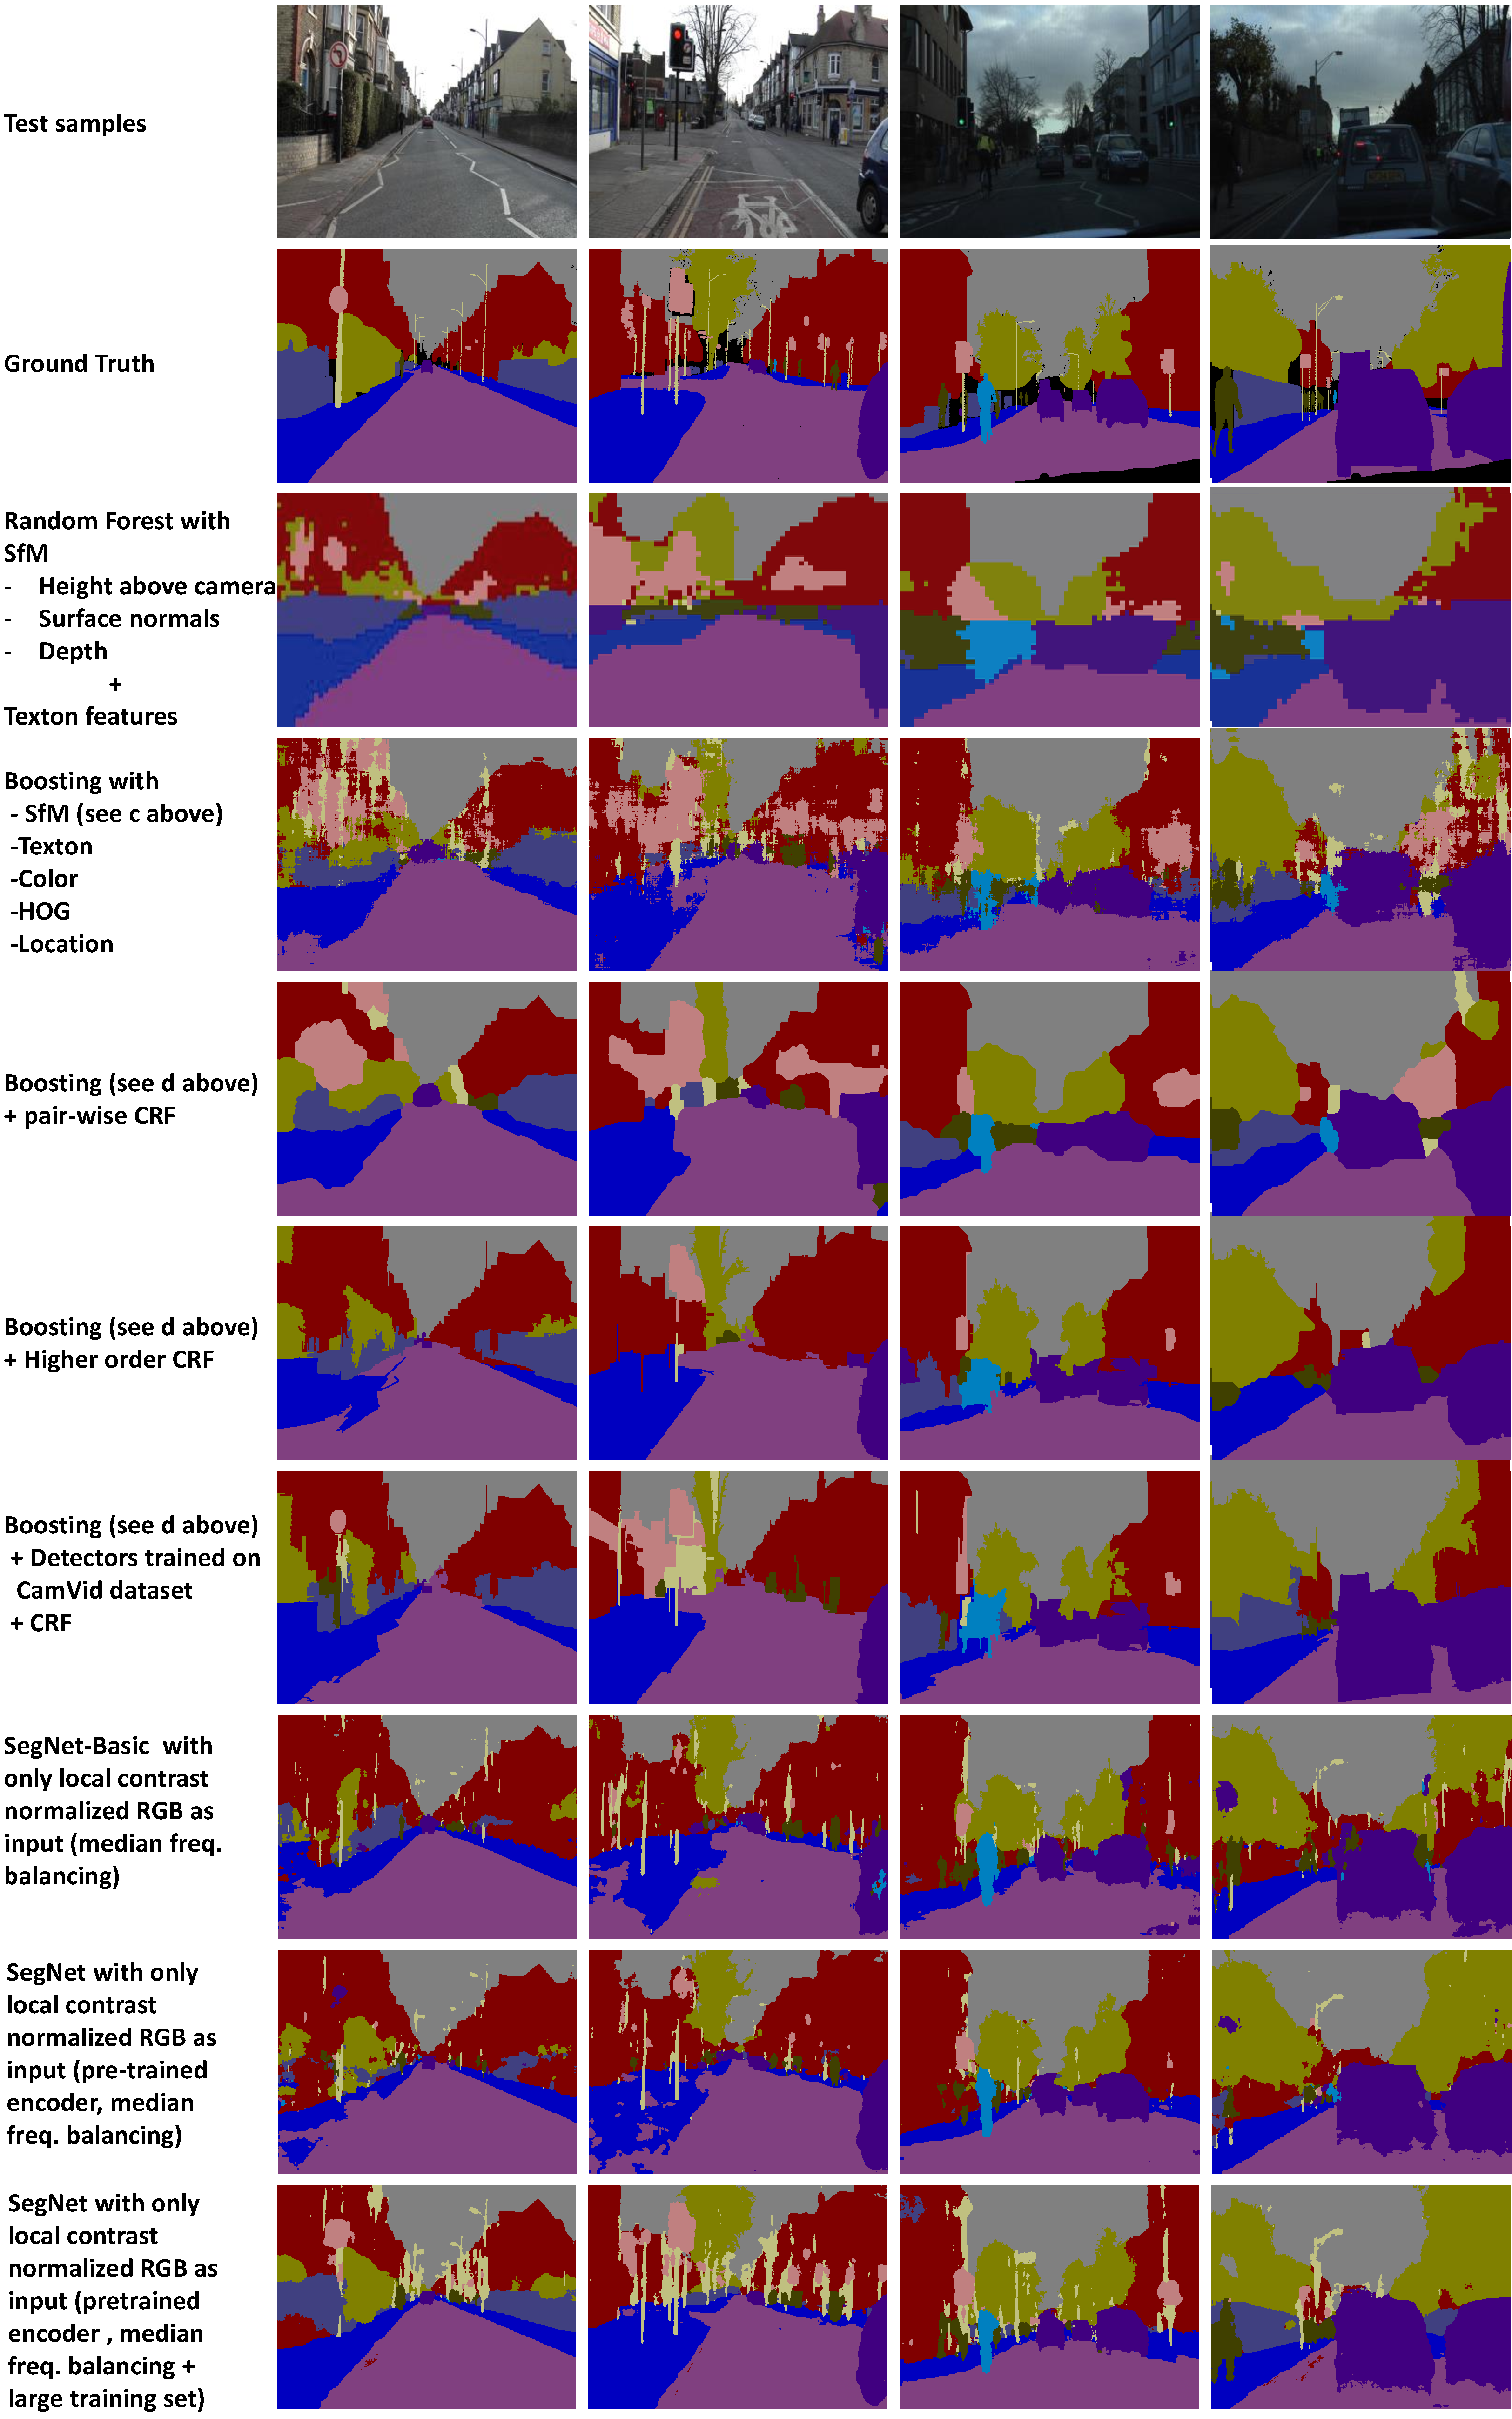
\includegraphics[width=0.85\textwidth]{segnet/CamVidQualitative.pdf}
\caption[CamVid qualitative results.]{Results on CamVid day and dusk test samples. The evolution of results from various patch based predictions \citep{Jamie2,brostow2008segmentation}, then CRF smoothing models \citep{LadickyECCV,Sturgess} and finally SegNet.
}
\label{CamVidQualy}
\end{figure*}

\subsubsection{CamVid Road Scenes}
\label{CamVid}
A number of outdoor scene datasets are available for semantic parsing \citep{gould2009decomposing,russell2008labelme,brostow2009semantic,Geiger2012CVPR}. From these, we choose to benchmark SegNet using the CamVid dataset \citep{brostow2009semantic} because it contains video sequences. This enables us to compare our proposed architecture with those which use motion and structure \citep{LadickyECCV,Sturgess,brostow2008segmentation} and video segments \citep{tighe2013superparsing}. We also combine \citep{gould2009decomposing,russell2008labelme,brostow2009semantic,Geiger2012CVPR} to form an ensemble of 3433 images to train SegNet for an additional benchmark.

The qualitative comparisons of SegNet-Basic and SegNet predictions with several prominent algorithms (unaries, unaries+CRF) are shown in \cref{CamVidQualy} along with the input modalities used to train the methods. The qualitative results show the ability of the proposed architectures to segment small (cars, pedestrians, bicyclist) classes while producing a smooth segmentation of the overall scene. The unary-only methods (like Random Forests or Boosting) which are trained to predict the label of the centre-pixel of a small patch produce low quality segmentations. Smoothing unaries with CRF's improve the segmentation quality considerably with higher order CRF's performing best. Although the CRF based results appear smooth, upon close scrutiny, we see that shape segmentation of smaller but important classes such as bicyclists, pedestrians are poor. In addition, natural shapes of classes like trees are not preserved and the details like the wheels of cars are lost.  More dense CRF models \citep{koltun2011efficient} can be better but with additional cost of inference. SegNet-Basic and SegNet (without large dataset training) clearly indicate their ability to retain the natural shapes of classes such as bicyclists, cars, trees, poles etc better than CRF based approaches. The overall segmentation quality is also smooth except for the side-walk class. This is because the side-walk class is highly varied in terms of size and texture and this cannot be captured with a small training set. Another explanation could be that the size of the receptive fields of the deepest layer feature units are smaller than their theoretical estimates \citep{zhou2014object,ParseNetRabinovich} and hence unable to group all the side-walk  pixels into one class. Illumination variations also affect performance on cars in the dusk examples. However, several of these issues can be ameliorated by using larger amounts of training data. In particular, we see that smaller classes such as pedestrians, cars, bicyclists, column-pole are segmented better than other methods in terms of shape retention. The side-walk class is also segmented smoothly.


\afterpage{%
    \clearpage% Flush earlier floats (otherwise order might not be correct)
    \begin{landscape}% Landscape page
\begin{table*}[th]
 \resizebox{\linewidth}{!}{
\small{
\begin{tabular}{c|c|c|c|c|c|c|c|c|c|c|c|ccc}

\multicolumn{1}{c}{Method}                   & \multicolumn{1}{c}{\rotatebox{90}{Building}} & \multicolumn{1}{c}{\rotatebox{90}{Tree}} & \multicolumn{1}{c}{\rotatebox{90}{Sky}}  & \multicolumn{1}{c}{\rotatebox{90}{Car}}  & \multicolumn{1}{c}{\rotatebox{90}{Sign-Symbol}} & \multicolumn{1}{c}{\rotatebox{90}{Road}} & \multicolumn{1}{c}{\rotatebox{90}{Pedestrian}} & \multicolumn{1}{c}{\rotatebox{90}{Fence}} & \multicolumn{1}{c}{\rotatebox{90}{Column-Pole}} & \multicolumn{1}{c}{\rotatebox{90}{Side-walk}} & \multicolumn{1}{c}{\rotatebox{90}{Bicyclist}} & \multicolumn{1}{c}{\rotatebox{90}{Class avg.}} & \multicolumn{1}{c}{\rotatebox{90}{Global avg.}} & \multicolumn{1}{c}{\rotatebox{90}{Mean IoU}}\\ \hline \hline



SfM+Appearance  \citep{brostow2008segmentation}           & 46.2     & 61.9 & 89.7 & 68.6 & 42.9        & 89.5 & 53.6       & 46.6  & 0.7         & 60.5     & 22.5      & 53.0       & 69.1  & n/a      \\ \hline

Boosting    \citep{Sturgess}              & 61.9     & 67.3 & 91.1 & 71.1 & 58.5        & 92.9 & 49.5       & 37.6  & 25.8        & 77.8     & 24.7      & 59.8       & 76.4  & n/a      \\ \hline

Dense Depth Maps   \citep{zhang2010semantic}          & 85.3     & 57.3 & 95.4 & 69.2 & 46.5        & \textbf{98.5} & 23.8       & 44.3  & 22.0        & 38.1     & 28.7      & 55.4       & 82.1    & n/a    \\ \hline

Structured Random Forests \citep{kontschieder2011structured}& \multicolumn{11}{c|}{n/a}                                                                          & 51.4       & 72.5    & n/a    \\ \hline

Neural Decision Forests \citep{BuloNeural}  & \multicolumn{11}{c|}{n/a}                                                                          & 56.1       & 82.1   & n/a     \\ \hline

Local Label Descriptors  \citep{yang2012local}  & 80.7     & 61.5 & 88.8 & 16.4 & n/a         & 98.0 & 1.09       & 0.05  & 4.13        & 12.4     & 0.07      & 36.3       & 73.6    & n/a    \\ \hline

Super Parsing   \citep{tighe2013superparsing}           & 87.0     & 67.1 & 96.9 & 62.7 & 30.1        & 95.9 & 14.7       & 17.9  & 1.7         & 70.0     & 19.4      & 51.2       & 83.3    & n/a    \\ \hline
SegNet-Basic          &  81.3    & 72.0  & 93.0 & 81.3 & 14.8 & 93.3 & 62.4 & 31.5 & 36.3  & 73.7 & 42.6  &   62.0    & 82.7   &   47.7   \\ \hline
SegNet-Basic (layer-wise training \citep{SegNetarXiv})         & 75.0     & 84.6 & 91.2 & 82.7 & 36.9        & 93.3 & 55.0       & 37.5  & 44.8        & 74.1     & 16.0      & 62.9       & 84.3   & n/a     \\ \hline
SegNet    &  \textbf{88.8}   & 87.3 & 92.4  & 82.1 & 20.5 & 97.2 &  57.1 & 49.3  &  27.5       &  84.4   &  30.7     &   65.2    &  \textbf{88.5}  & 55.6     \\ \hline
SegNet (3.5K dataset training)   & 73.9  & \textbf{90.6}  & 90.1  & \textbf{86.4}  &  \textbf{69.8}  & 94.5 &   \textbf{86.8}   & \textbf{67.9}  &   \textbf{74.0}	   &  \textbf{94.7}	   &  \textbf{52.9}    & \textbf{80.1}  & 86.7 &       \textbf{60.4}\\ \hline

\multicolumn{15}{c}{CRF based approaches}                                                                                                       \\ \hline

Boosting + pairwise CRF  \citep{Sturgess} & 70.7     & 70.8 & 94.7 & 74.4 & 55.9        & 94.1 & 45.7       & 37.2  & 13.0        & 79.3     & 23.1      & 59.9       & 79.8  & n/a      \\ \hline

Boosting+Higher order \citep{Sturgess}    & 84.5     & 72.6 & \textbf{97.5} & 72.7 & 34.1        & 95.3 & 34.2       & 45.7  & 8.1         & 77.6     & 28.5      & 59.2       & 83.8    & n/a    \\ \hline

Boosting+Detectors+CRF \citep{LadickyECCV}   & 81.5     & 76.6 & 96.2 & 78.7 & 40.2        & 93.9 & 43.0       & 47.6  & 14.3        & 81.5     & 33.9      & 62.5       & 83.8    & n/a    \\ \hline
\end{tabular}
}}
\caption[CamVid quantitative results.]{Quantitative results on CamVid \citep{brostow2009semantic} consisting of 11 road scene categories. SegNet outperforms all the other methods, including those using depth, video and/or CRF's. In comparison with the CRF based methods SegNet predictions are more accurate in 8 out of the 11 classes. It also shows a good $\approx 15\%$ improvement in class average accuracy when trained on a large dataset of 3.5K images and this sets a new benchmark for the majority of the individual classes. Particularly noteworthy are the significant improvements in accuracy for the smaller/thinner classes. 
}
\label{CamVidQuant}
\end{table*}
\end{landscape}}

The quantitative results in Table \ref{CamVidQuant} show SegNet-Basic and SegNet obtain competitive results, even without CRF based processing. This shows the ability of the deep architecture to extract meaningful features from the input image and map it to accurate and smooth class segment labels. SegNet is better in performance than SegNet-Basic although trained with the same (small) training set. This indicates the importance of using pre-trained encoder weights and a deeper architecture. Interestingly, the use of the bigger and deeper SegNet architecture improves the accuracy of the larger classes as compared to SegNet-Basic and not the smaller classes as one might expect. We also find that SegNet-Basic \citep{SegNetarXiv} trained in a layer-wise manner using L-BFGS \citep{Nocedal} also performs competitively and is better than SegNet-Basic trained with SGD (see Sec. \ref{Training}). This is an interesting training approach but needs further research in order for it scale to larger datasets.

The most interesting result is the approximately $15\%$ performance improvement in class average accuracy that is obtained with a large training dataset, obtained by combining \citet{gould2009decomposing}, \citet{russell2008labelme}, \citet{brostow2009semantic} and \citet{Geiger2012CVPR}. The mean of intersection over union metric is also very high. Correspondingly, the qualitative results of SegNet (see \cref{CamVidQualy}) are clearly superior to the rest of the methods. It is able to segment both small and large classes well. In addition, there is an overall smooth quality of segmentation much like what is typically obtained with CRF post-processing. Although the fact that results improve with larger training sets is not surprising, the percentage improvement obtained using a pre-trained encoder network and this training set indicates that this architecture can potentially be deployed for practical applications. Our random testing on urban and highway images from the internet (see \cref{Teaser}) demonstrates that SegNet can \textit{absorb} a large training set and generalize well to unseen images. It also indicates the contribution of the prior (CRF) can be lessened when sufficient amount of training data is made available.

\subsubsection{SUN RGB-D Indoor Scenes}
\label{SUNRGBD}

\begin{figure*}
\centering
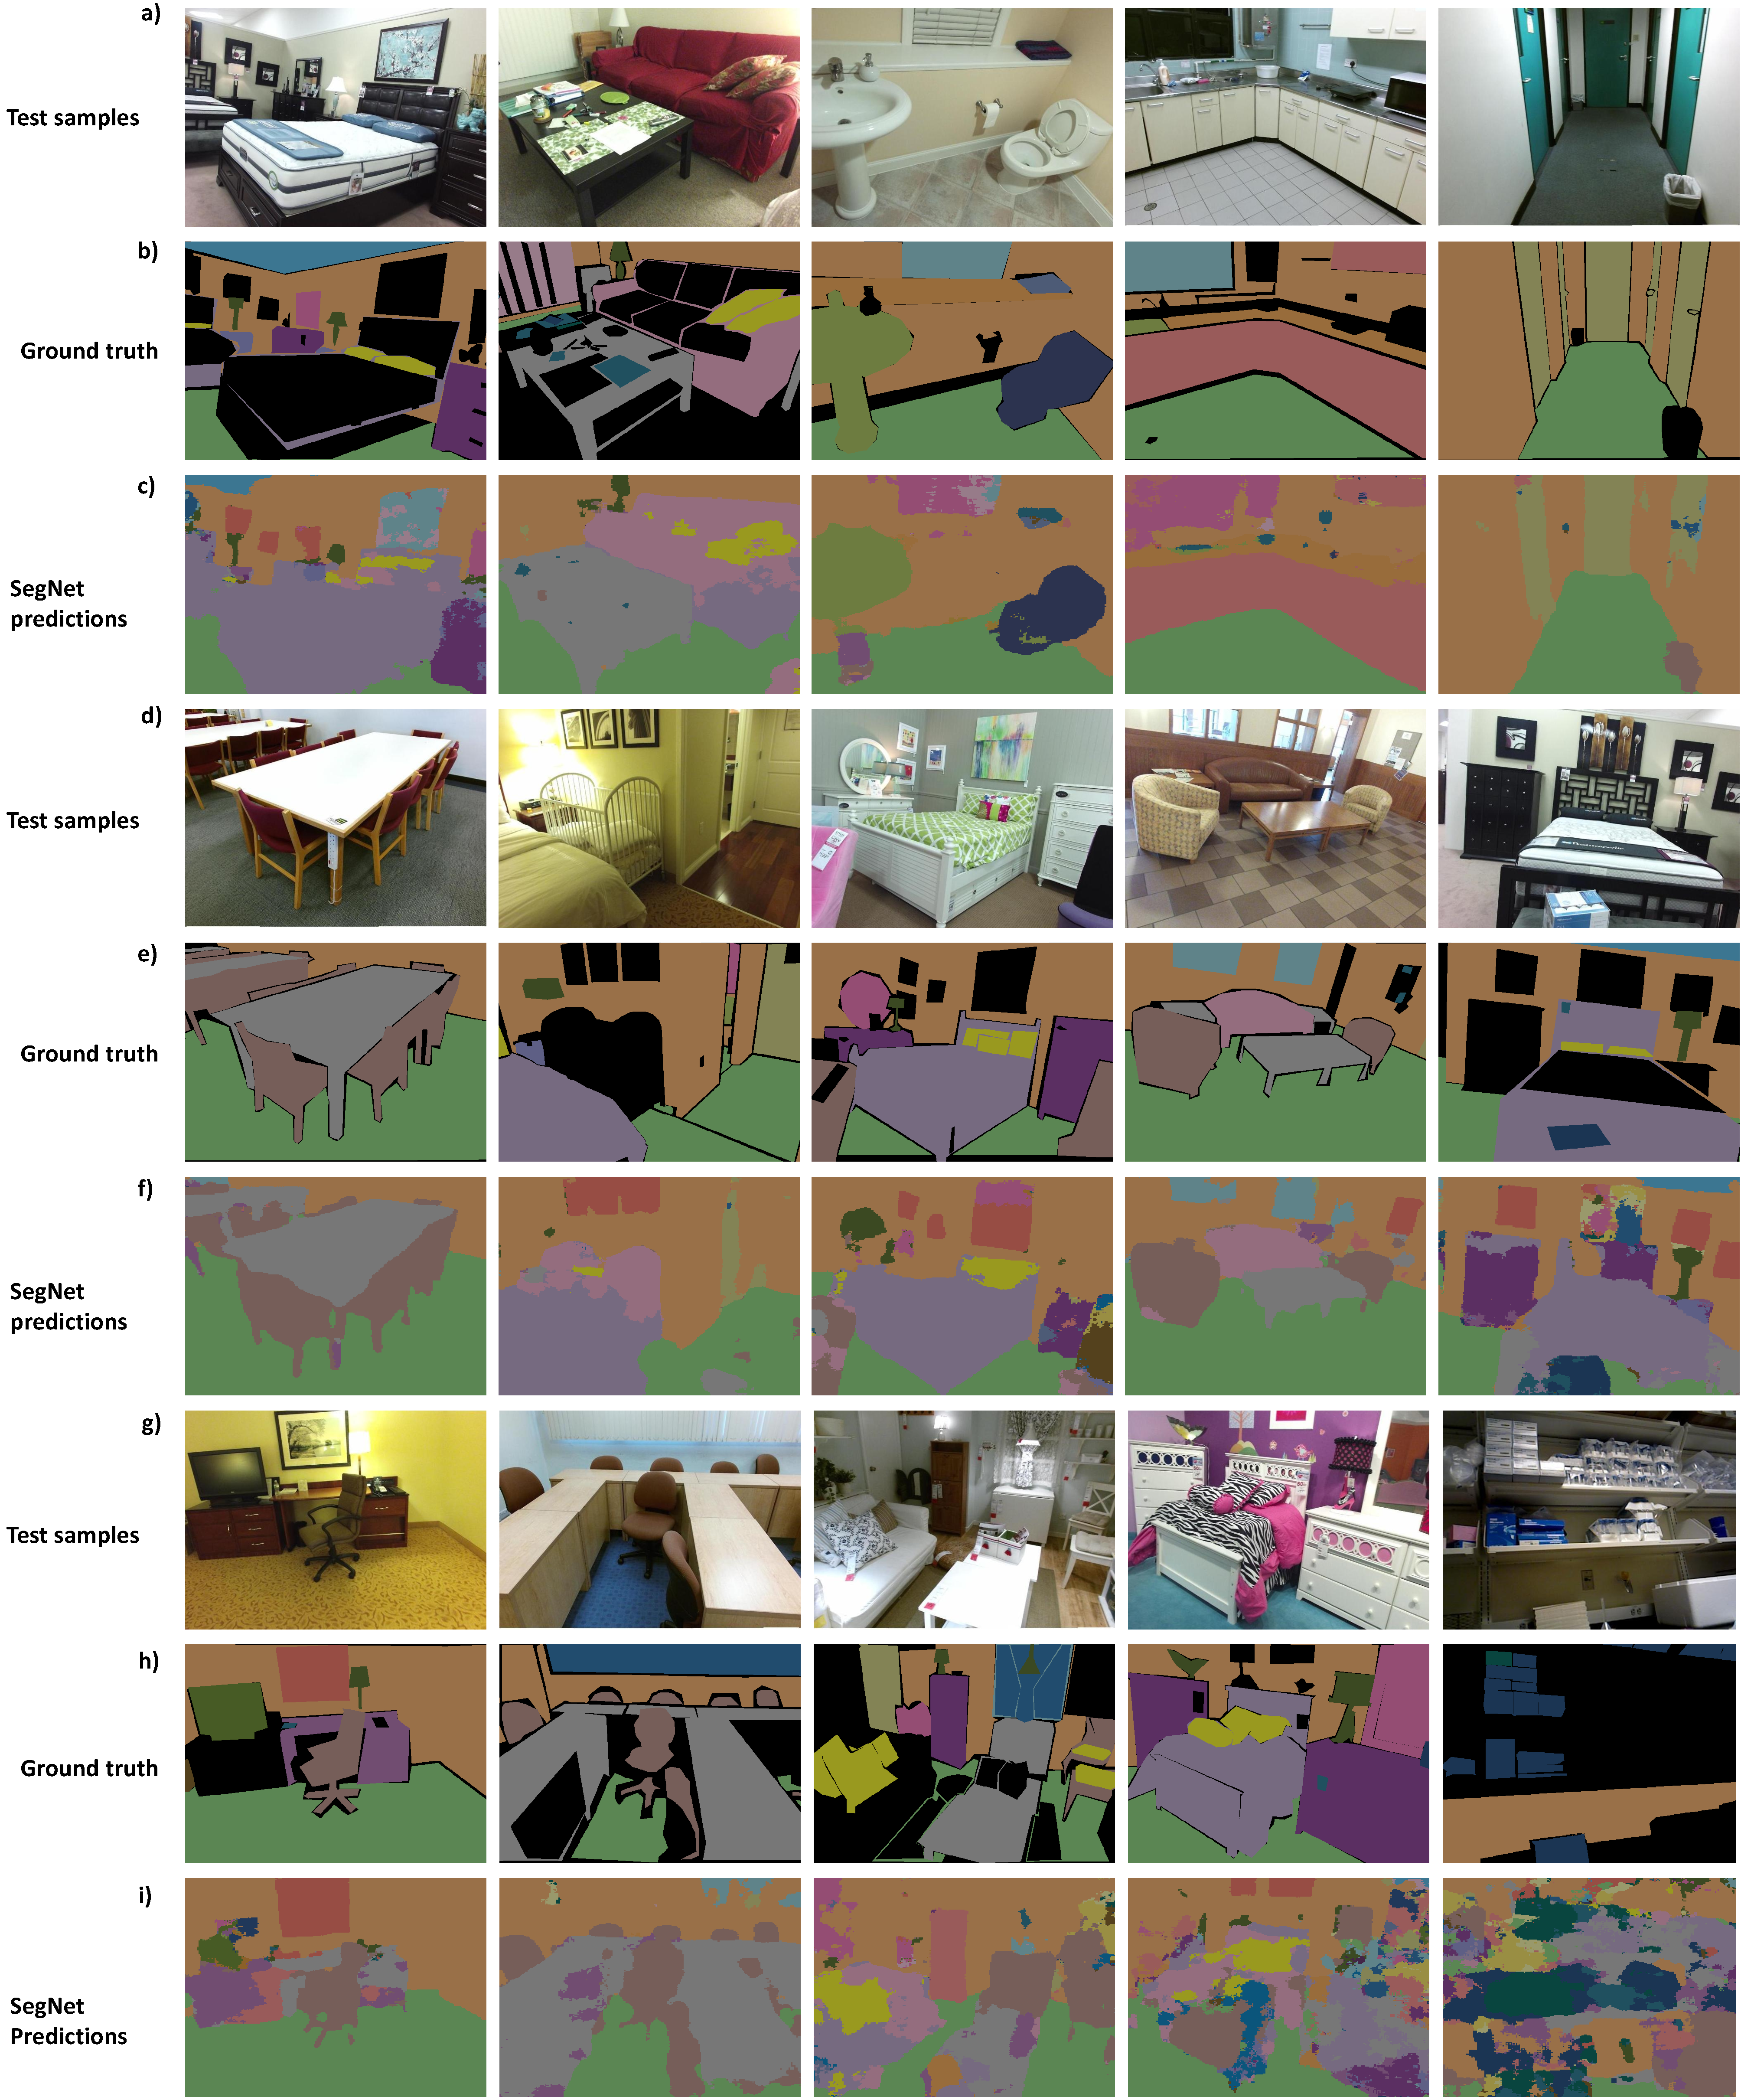
\includegraphics[width=\textwidth]{segnet/SUNRGBDQualy2.pdf}
\caption[SegNet qualitative results on RGB-D dataset.]{Qualitative assessment of SegNet predictions on RGB indoor test scenes from the recently released SUN RGB-D dataset \citep{song2015sun}. In this hard challenge, SegNet predictions delineate inter class boundaries well for object classes in a variety of scenes and their view-points. The segmentation quality is good when object classes are reasonably sized (rows (c,f)) but suffers when the scene is more cluttered (last two samples in row (i)). Unlabelled regions are shown as black in the ground truth.}
\label{SUNRGBDQualy}
\end{figure*}

Road scene images have limited variation, both in terms of the classes of interest and their spatial arrangements, especially when captured in a single sequence from a moving vehicle. In comparison, images of indoor scenes are more complex since the view points can vary significantly and there is less regularity in both the number of classes present in a scene and their spatial arrangement. Another difficulty is caused by the widely varying sizes of the object classes in the scene. Some test samples from the recent SUN RGB-D dataset \citep{song2015sun} are shown in \cref{SUNRGBDQualy}. We observe some scenes with few large classes and some others with dense clutter (bottom row and right). The appearance (texture and shape) can also widely vary in indoor scenes. Therefore, we believe this is the hardest challenge for segmentation architectures and methods in computer vision. Other challenges such as Pascal VOC12 \citep{pascal} salient object segmentation have occupied researchers, but indoor scene segmentation is more challenging and has more practical applications such as in robotics. Our model advances state-of-the-art on the large SUN RGB-D dataset.

The qualitative results of SegNet on some images of indoor scenes of different types such as bedroom, kitchen, bathroom, classroom etc. are shown in \cref{SUNRGBDQualy}. We see that SegNet obtains sharp boundaries between classes when the scene consists of reasonable sized classes but even when viewpoint changes are present (see bed segmentation from different view points). This is particularly interesting since the input modality is only RGB. It indicates the ability of SegNet to extract features from RGB images which are useful for view-point invariant segmentation provided there is sufficient training data (here 5285 images). RGB images are also useful to segment thinner structures such as the legs of chairs and tables, lamps which is difficult to achieve using depth images from currently available sensors. It is also useful to segment decorative objects such as paintings on the wall. 

In Table \ref{SUNRGBDtest} we report the quantitative results on the $37$ class segmentation task. We first note here that the other methods that have been benchmarked are not based on deep architectures and they only report class average accuracy. The existing top performing method \citep{ren2012rgb} relies on hand engineered features using colour, gradients and surface normals for describing super-pixels and then smooths super-pixel labels with a CRF. For SegNet we achieve a high global accuracy which correlates with an overall smooth segmentation. This also suggests that largest classes such as wall, floor, bed, table, sofa are segmented well in spite of view-point changes and appearance variations. However, the class average accuracy and mean IoU metric are poor, but at the same level as the hand engineered method which also includes the depth channel as input. This shows that smaller and thinner classes which have lesser training data are not segmented well. The individual class accuracies are reported in Table \ref{SUNRGBDClassavg}. From these we see that there is a clear correlation between the size and natural frequency of occurrence of classes and their individual accuracies. It is also informative to note RGB input is useful to segment widely varying (shape, texture) categories such as wall, floor, ceiling, table, chair, sofa with reasonable accuracy.

\begin{table}[t]
\centering
\begin{tabular}{c|ccc}
%\hline
{Method} & {Global avg.} & {Class avg.} & {Mean IoU} \\ \hline \hline
\multicolumn{4}{c}{RGB}                                                        \\ \hline
Liu \emph{et~al.}  \citep{SIFT_flow}      & n/a                  & 9.3                & n/a               \\ \hline
SegNet            & \textbf{70.3}                & 35.6               & \textbf{26.3}            \\ \hline
\multicolumn{4}{c}{RGB-D}                                                       \\ \hline
Liu \emph{et~al.}   \citep{SIFT_flow}    & n/a                  & 10.0               & n/a               \\ \hline
Ren et. al \citep{ren2012rgb}     & n/a                  & \textbf{36.3}               & n/a               \\ \hline
\end{tabular}
\caption[SegNet quantitative results on the SUN RGB-D dataset.]{Quantitative comparison on the SUN RGB-D dataset which consists of 5050 test images of indoor scenes with 37 classes. SegNet RGB-based predictions have a high global accuracy and also match the RGB-D based predictions \citep{ren2012rgb} in terms of class average accuracy.}
\label{SUNRGBDtest}
\end{table}

\begin{table*}[t]
\centering
\tabcolsep=3pt
 \resizebox{\textwidth}{!}{
\begin{tabular}{c|c|c|c|c|c|c|c|c|c|c|c|c}
%\hline
\multicolumn{1}{c|}{Wall} & \multicolumn{1}{c|}{Floor} & \multicolumn{1}{c|}{Cabinet} & \multicolumn{1}{c|}{Bed} & \multicolumn{1}{c|}{Chair} & \multicolumn{1}{c|}{Sofa} & \multicolumn{1}{c|}{Table} & \multicolumn{1}{c|}{Door} & \multicolumn{1}{c|}{Window} & \multicolumn{1}{c|}{Bookshelf} & \multicolumn{1}{c|}{Picture} & \multicolumn{1}{c|}{Counter} & \multicolumn{1}{c}{Blinds} \\ \hline
86.6                       & 92.0                       & 52.4                         & 68.4                     & 76.0                       & 54.3                      & 59.3                       & 37.4                      & 53.8                        & 29.2                           & 49.7                         & 32.5                         & 31.2                        \\ \hline
Desk                       & Shelves                    & Curtain                      & Dresser                  & Pillow                     & Mirror                    & Floor mat                  & Clothes                   & Ceiling                     & Books                          & Fridge                       & TV                           & Paper                       \\ \hline
17.8                       & 5.3                        & 53.2                         & 28.8                     & 36.5                       & 29.6                      & 0.0                        & 14.4                      & 67.7                        & 32.4                           & 10.2                         & 18.3                         & 19.2                        \\ \hline
Towel                      & Shower curtain             & Box                          & Whiteboard               & Person                     & Night stand               & Toilet                     & Sink                      & Lamp                        & Bathtub                        & Bag                          & \multicolumn{2}{c}{\multirow{2}{*}{}}                     \\ \cline{1-11}
11.5                       & 0.0                        & 8.9                          & 38.7                     & 4.9                        & 22.6                      & 55.6                       & 52.7                      & 27.9                        & 29.9                           & 8.1                          & \multicolumn{2}{c}{}                                      \\ \cline{1-11}
\end{tabular}}
\caption[SegNet class accuracy on SUN RGB-D.]{Class average accuracy of SegNet predictions for the 37 indoor scene classes in the SUN RGB-D benchmark dataset.}
\label{SUNRGBDClassavg}
\end{table*}

\subsubsection{Pascal VOC12 Segmentation Challenge}
\label{Pascal}
The Pascal VOC12 segmentation challenge \citep{pascal} consists of segmenting a few salient object classes from a widely varying background class. It is unlike the segmentation for scene understanding benchmarks described earlier which require learning both classes and their spatial context. A number of techniques have been proposed based on this challenge which are increasingly more accurate and complex.\footnote{\label{pascallb} See the leader board at \url{http://host.robots.ox.ac.uk:8080/leaderboard}} Our efforts in this benchmarking experiment have not been diverted towards attaining the top rank by either using multi-stage training \citep{long2015fully}, other datasets for pre-training such as MS-COCO \citep{lin2014microsoft, CRFRNN}, training and inference aids such as object proposals \citep{zitnick2014edge, NohDeconvNets} or post-processing using CRF based methods \citep{chen2016deeplab, NohDeconvNets}.  Although these supporting techniques clearly have value towards increasing the performance it unfortunately does not reveal the true performance of the deep architecture which is the \textit{core segmentation engine}. It however does indicate that some of the large deep networks are difficult to train end-to-end on this task even with pre-trained encoder weights. Therefore, to encourage more controlled benchmarking, we trained SegNet end-to-end without other aids and report this performance. 

In Table \ref{PascalQuant} we show the class average accuracy for some recent methods based on deep architectures. To the best of our ability, we have tried to gather the performance measures of the competing methods for their runs using minimum supporting techniques. We also specify when a method reports the performance of its core engine on the smaller validation set of $346$ images \citep{chen2016deeplab}. We find the performance on the full test set to be approximately  $1\%$ less as compared to the smaller validation set. 


\begin{figure*}[t]
\centering
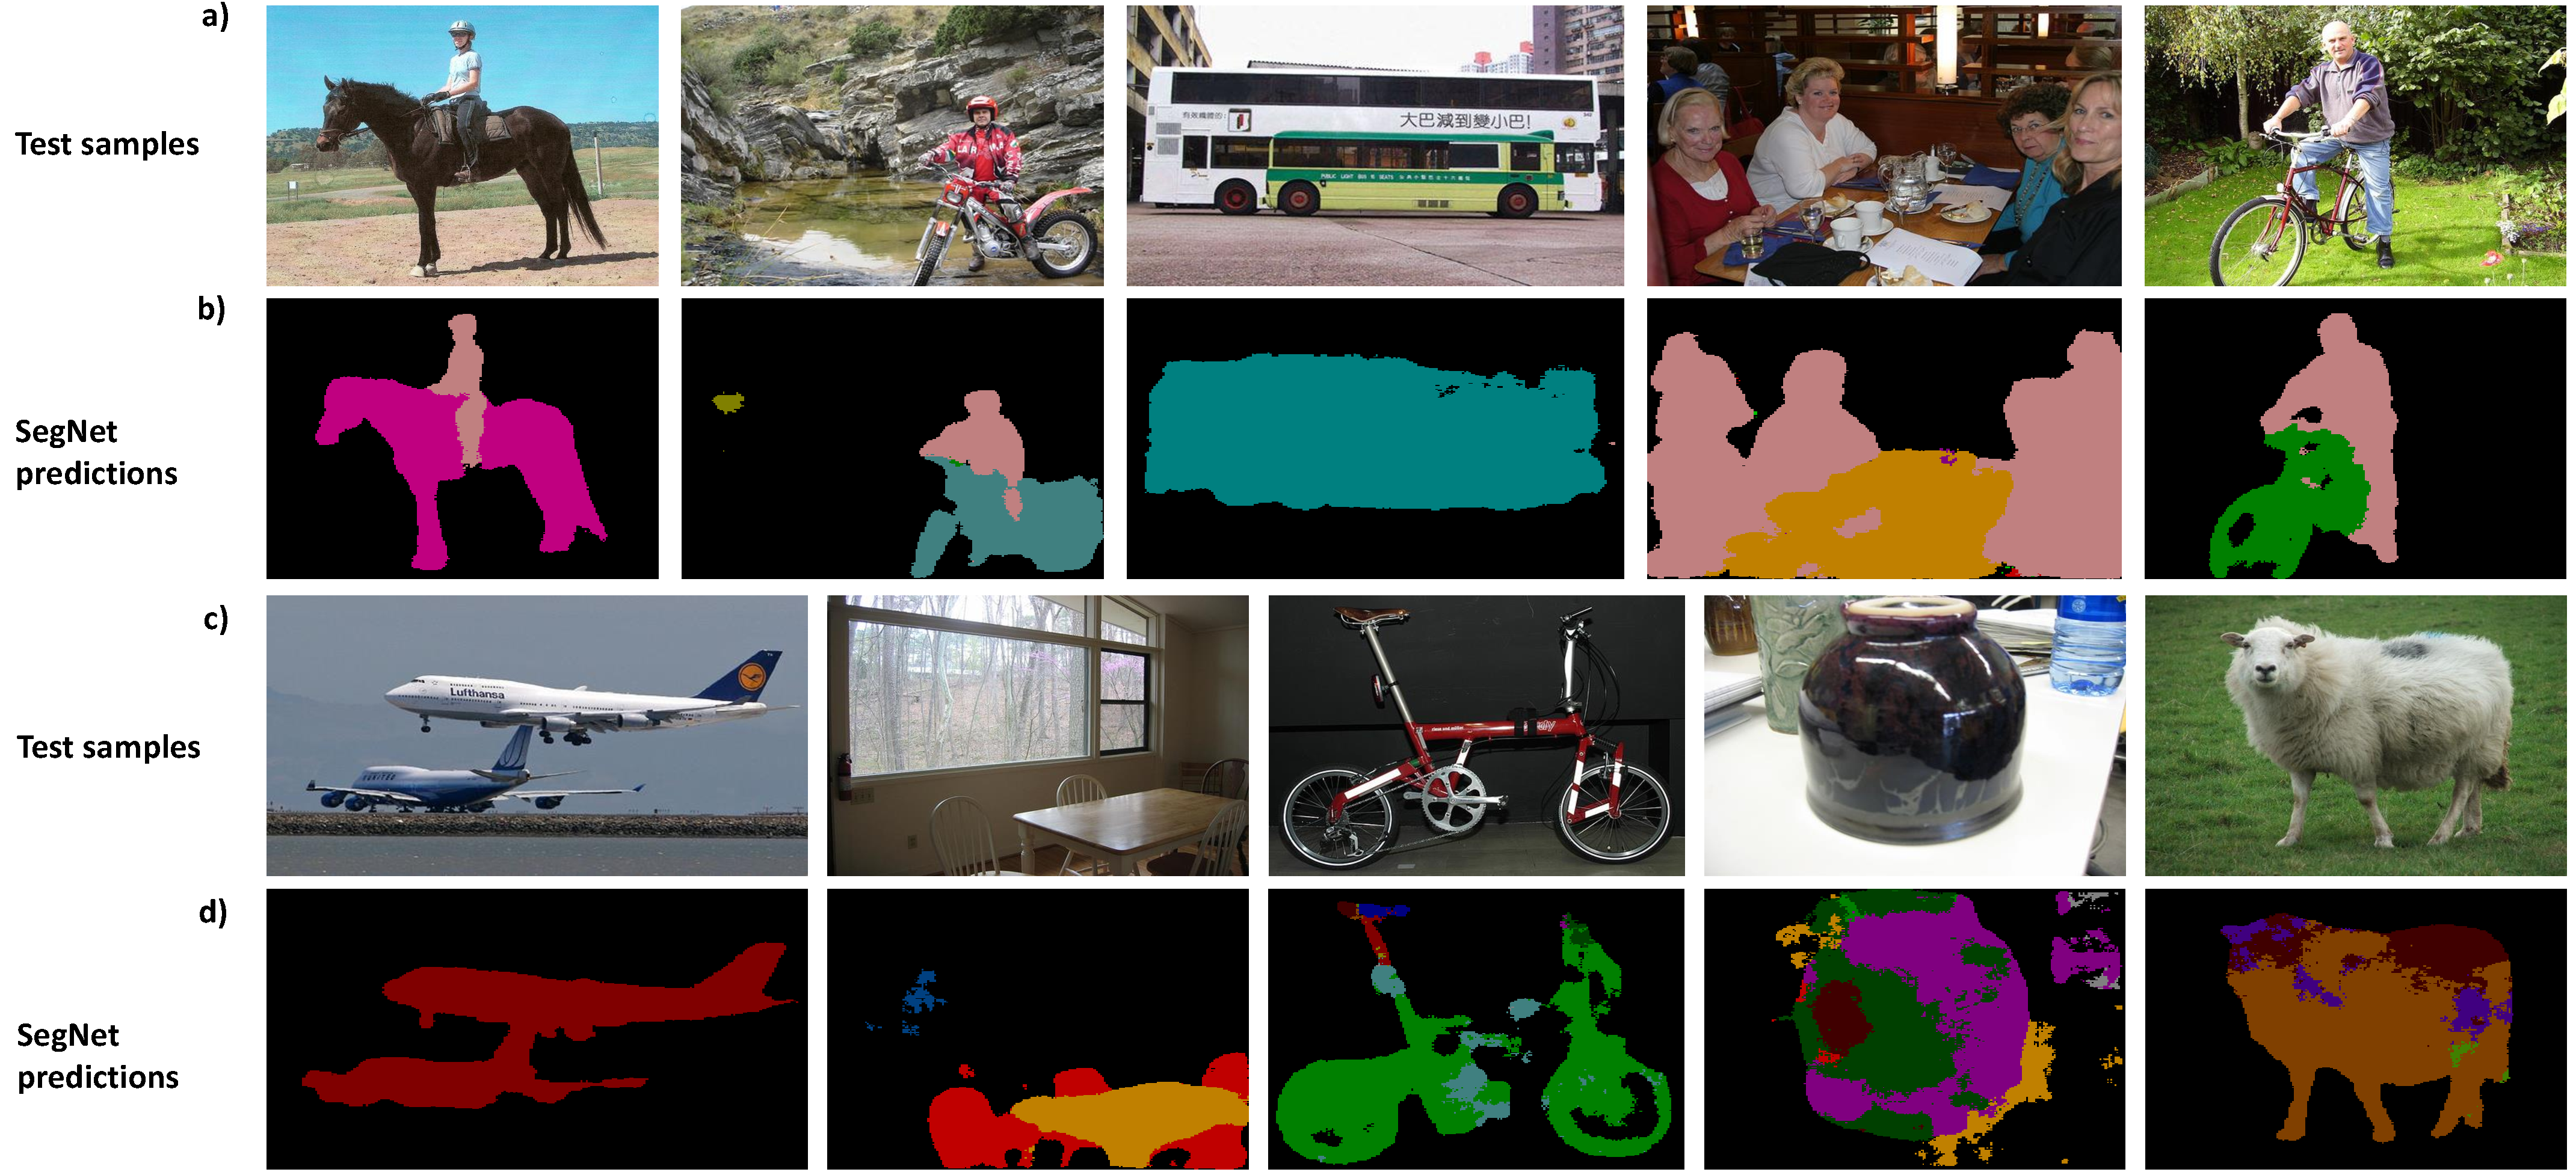
\includegraphics[width=\textwidth]{segnet/PascalQualy2.pdf}
\caption[Qualitative assessment of SegNet on Pascal VOC12]{Qualitative assessment of SegNet predictions on test samples from the Pascal VOC12 \citep{pascal} dataset. SegNet performs competitively (row (b) on several object classes of varying shape and appearance. However, it lacks smoothness particularly on large objects (see row(d)). This can be perhaps be attributed to the smaller empirical size of the receptive field of the feature units in the deepest encoder layer size \citep{zhou2014object}.}
\label{PascalQualy}
\end{figure*}

\afterpage{%
    \begin{landscape}% Landscape page
\begin{table*}[]
\centering
\resizebox{\linewidth}{!}{
\tabcolsep=2pt
\begin{tabular}{c|c|c|c|c|c|c}
\hline
Method       & Encoder size (M) & Decoder size (M) & Total size (M) & Class avg. acc. & Inference $500 \times 500$ pixels & Inference $224 \times 224$ pixels \\ \hline \hline
chen2016deeplab \citep{chen2016deeplab} (validation set)  & n/a & n/a & $<$ 134.5 & 58   & n/a & n/a       \\ \hline
FCN-8 \citep{long2015fully}  (multi-stage training)  & 134 & \textbf{0.5} & 134.5 & 62.2  & 210ms & n/a       \\ \hline
Hypercolumns \citep{hariharan2015hypercolumns}  (object proposals) & n/a & n/a & $>$ 134.5 & 62.6  & n/a & n/a            \\ \hline
DeconvNet \citep{NohDeconvNets} (object proposals) &  138.35 & 138.35 & 276.7 & 69.6  & n/a & 92ms ($\times$ 50)        \\ \hline  
CRF-RNN \citep{CRFRNN} (multi-stage training)                  & n/a & n/a & $>$ 134.5 & \textbf{69.6} & n/a & n/a     \\ \hline
SegNet       & \textbf{14.725}       & 14.725 & \textbf{29.45} & 59.1   & \textbf{94ms}  & \textbf{28ms}  \\ \hline
\end{tabular}
}
\caption[SegNet performance on Pascal VOC 2012]{Quantitative comparison on Pascal VOC12 dataset. The accuracies for the competing architectures are gathered for their inference run using the least number of supporting training and inference techniques. However, since they are not trained end-to-end like SegNet and use aids such as object proposals, we have added corresponding qualifying comments. The first three columns show the number of trainable parameters in the encoder, decoder and full  network. Many of the models are approximately the same size as FCN. In comparison, SegNet is considerably smaller but achieves a competitive accuracy without resorting to supporting training or inference aids. This results in SegNet being significantly faster than other models in terms of inference time.}
\label{PascalQuant}
\end{table*}
\end{landscape}}

From the results in Table \ref{PascalQuant} we can see that the best performing networks are either very large (and slow) \citep{NohDeconvNets} and/or they use a CRF \citep{CRFRNN}. The CRF encourages large segments with a single label and this suits the Pascal challenge wherein there are one or two salient objects in the centre of the image. This prior also has a larger impact when training data is limited. This is shown in the experiments using CRF-RNN  \citep{CRFRNN} wherein the core FCN-8 model predictions are less accurate without extra training data. 

It is interesting that the DeepLab \citep{chen2016deeplab} architecture which is simply upsampling the FCN encoder features using bilinear interpolation performs reasonably well (on the validation set). The fact that a coarse segmentation is enough to produce this performance shows that this challenge is unlike scene understanding wherein many classes of varying shape and size need to be segmented.

Methods using object proposals during training and/or inference \citep{NohDeconvNets,hariharan2015hypercolumns} are very slow in inference time and it is hard to measure their true performance. These aids are necessitated by the very large size of their deep network \citep{NohDeconvNets} and also because the Pascal data can also be processed by a detect and segment approach. In comparison, SegNet is smaller by virtue of discarding the fully connected layers in the VGG16 \citep{simonyan2014very}. The authors of DeepLab \citep{chen2016deeplab} have also reported little loss in performance by reducing the size of the fully connected layers. The smaller size of SegNet makes end-to-end training possible for benchmarking. Although it may be argued that larger networks perform better, it is at the cost of a complex training mechanism, increased memory and inference time. This makes them unsuitable for real-time applications such as road scene understanding. 

The individual class accuracies for SegNet predictions on Pascal VOC12 are shown in Table \ref{PascalClassavg}. From this we once again see larger and more frequently occurring classes such as aeroplane, bus, cat \textit{etc}. have higher accuracy and smaller/thinner classes such as potted plant, bicycle are poorly segmented. We believe more training data \citep{lin2014microsoft} can help improve the performance of SegNet.

In the following section, we investigate techniques to improve our scene understanding algorithm by modelling uncertainty with deep learning.


\begin{table*}[t]
\centering
\resizebox{\linewidth}{!}{
\begin{tabular}{c|c|c|c|c|c|c|c|c|c|c}
\hline
Aeroplane & Bicycle & Bird & Boat & Bottle & Bus & Car & Cat & Chair & Cow & Dining table \\ \hline
74.5 & 30.6 & 61.4 & 50.8 & 49.8 & 76.2 & 64.3 & 69.7 & 23.8 & 60.8 & 54.7 \\ \hline
Dog  & Horse & Motor bike & Person & Potted plant & Sheep & Sofa & Train & TV & Background & \multirow{2}{*}{} \\ \cline{1-10}
62.0 & 66.4 & 70.2 & 74.1 & 37.5 & 63.7 & 40.6 & 67.8 & 53.0 & 88.6 & \\ \cline{1-10}
\end{tabular}}
\caption[Individual class accuracies of SegNet on Pascal VOC12]{Individual class accuracies of SegNet predictions on the Pascal VOC12 segmentation benchmark consisting of 21 object classes.}
\label{PascalClassavg}
\end{table*}









\section{Modelling Uncertainty}
\label{seg_unc}

The algorithms presented so far in this chapter produce accurate semantic segmentation predictions, however they are unaware of their uncertainty. Understanding what a model does not know is a critical part of many machine learning systems \citep{ghahramani2015probabilistic}.

Quantifying uncertainty in computer vision applications can be largely divided into regression settings such as depth regression, and classification settings such as semantic segmentation.
Existing approaches to model uncertainty in such settings in computer vision include particle filtering and conditional random fields \citep{blake1993framework, he2004multiscale}. However, many modern applications mandate the use of \textit{deep learning} to achieve state-of-the-art performance \citep{he2016deep}. Unfortunately, most deep learning models are not able to represent uncertainty.
For example, deep learning typically does not allow for uncertainty representation in regression settings. Deep learning classification models often give normalised score vectors, which do not necessarily capture model uncertainty. For both settings uncertainty can be captured with \textit{Bayesian deep learning} \citep{denker1991transforming, mackay1992practical, neal1995bayesian} approaches --
which offer a practical framework for understanding uncertainty with deep learning models 
\citep{gal2016thesis}.

In Bayesian modelling, there are two main types of uncertainty one can model \citep{der2009aleatory}. \textit{Aleatoric} uncertainty captures noise inherent in the observations.
This could be, for example, sensor noise or motion noise, resulting in uncertainty which cannot be reduced even if more data were to be collected.
On the other hand, \textit{epistemic} uncertainty accounts for uncertainty in the model parameters -- uncertainty which captures our ignorance about which model generated our collected data. 
This uncertainty can be explained away given enough data, and is often referred to as \textit{model uncertainty}. Aleatoric uncertainty can further be categorized into \textit{homoscedastic} uncertainty, uncertainty which stays constant for different inputs, and \textit{heteroscedastic} uncertainty. Heteroscedastic uncertainty depends on the inputs to the model, with some inputs potentially having more noisy outputs than others. 
Heteroscedastic uncertainty is especially important for computer vision applications. For example, for depth regression, highly textured input images with strong vanishing lines are expected to result in confident predictions, whereas an input image of a featureless wall is expected to have very high uncertainty.

In this section we make the observation that in many big data regimes (such as the ones common to deep learning with image data), it is most effective to model aleatoric uncertainty, uncertainty which cannot be explained away.
This is in comparison to epistemic uncertainty which is mostly explained away with the large amounts of data often available in machine vision.
We further show that modelling aleatoric uncertainty alone comes at a cost. Out-of-data examples, which can be identified with epistemic uncertainty, cannot be identified with aleatoric uncertainty alone.

For this we present a unified Bayesian deep learning framework which allows us to learn mappings from input data to aleatoric uncertainty and compose these together with epistemic uncertainty approximations. We derive our framework for both regression and classification applications and present results for per-pixel depth regression and semantic segmentation tasks (see \cref{fig:camvid_qual} for examples). 
We show how modelling aleatoric uncertainty in regression can be used to learn loss attenuation, and develop a complimentary approach for the classification case. 
This demonstrates the efficacy of our approach on difficult and large scale tasks.

The main contributions of this section are; 
\begin{enumerate}
\item We capture an accurate understanding of aleatoric and epistemic uncertainties, in particular with a novel approach for classification,
\item We improve model performance by $1-3\%$ over non-Bayesian baselines by reducing the effect of noisy data with the implied attenuation obtained from explicitly representing aleatoric uncertainty,
\item We study the trade-offs between modelling aleatoric or epistemic uncertainty by characterizing the properties of each uncertainty and comparing model performance and inference time.
\end{enumerate}

\begin{figure*}[t]
\centering
\resizebox{0.97\linewidth}{!}{
    \begin{subfigure}[t]{0.22\linewidth}
        \centering
		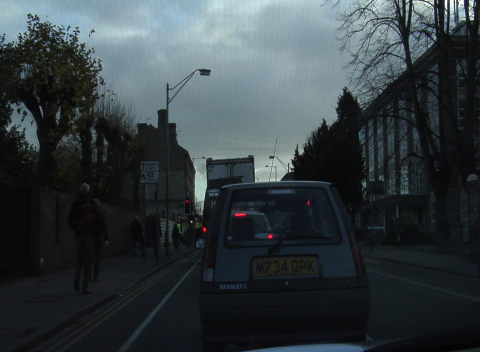
\includegraphics[width=\linewidth]{segnet_1_output_0.png}
        \vspace{1px}
		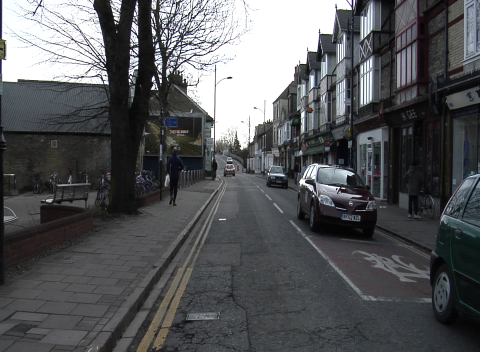
\includegraphics[width=\linewidth]{segnet_13_output_0.png}
        \vspace{1px}
        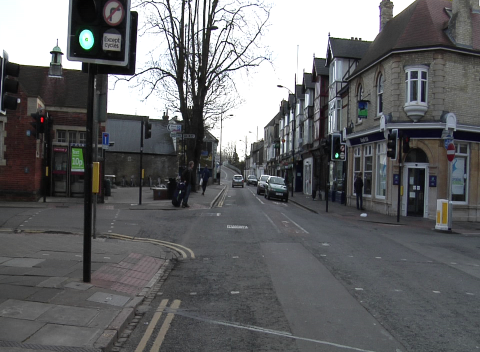
\includegraphics[width=\linewidth]{segnet_2_output_0.png}
        \caption{Input Image}
    \end{subfigure}
    \begin{subfigure}[t]{0.22\linewidth}
        \centering
		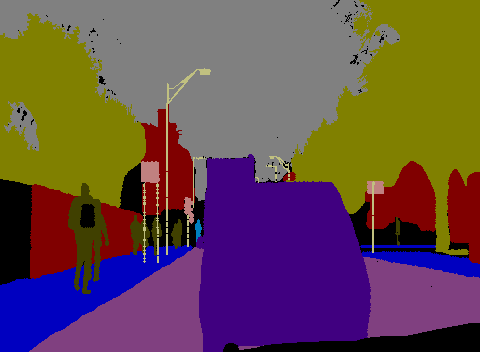
\includegraphics[width=\linewidth]{segnet_1_output_2.png}
        \vspace{1px}
		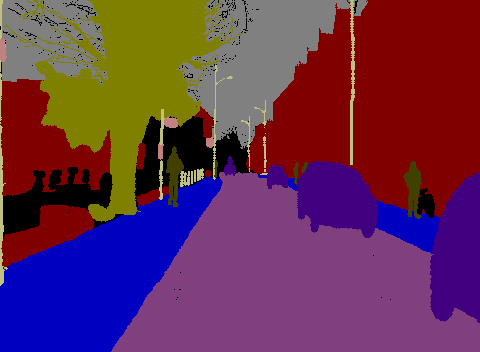
\includegraphics[width=\linewidth]{segnet_13_output_2.png}
        \vspace{1px}
        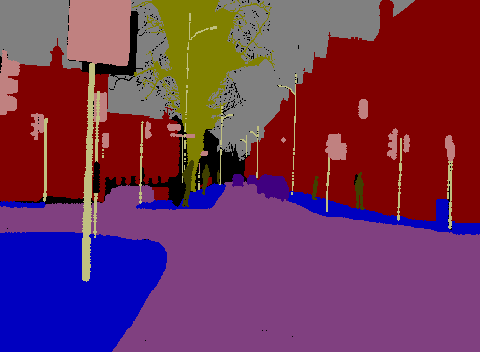
\includegraphics[width=\linewidth]{segnet_2_output_2.png}
        \caption{Ground Truth}
    \end{subfigure}
    \begin{subfigure}[t]{0.22\linewidth}
        \centering
		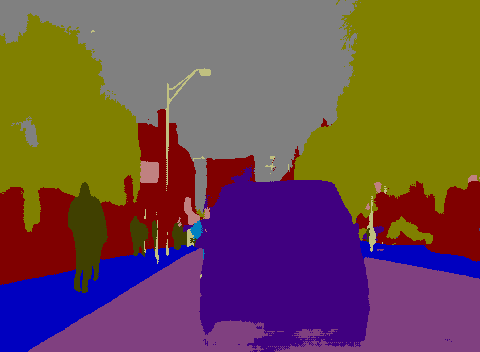
\includegraphics[width=\linewidth]{segnet_1_output_1.png}
        \vspace{1px}
		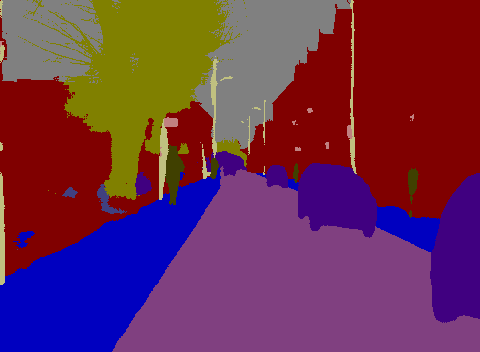
\includegraphics[width=\linewidth]{segnet_13_output_1.png}
        \vspace{1px}
        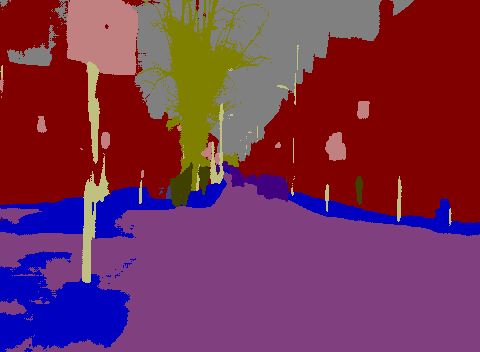
\includegraphics[width=\linewidth]{segnet_2_output_1.png}
        \caption{Semantic\\Segmentation}
    \end{subfigure}
    \begin{subfigure}[t]{0.22\linewidth}
        \centering
		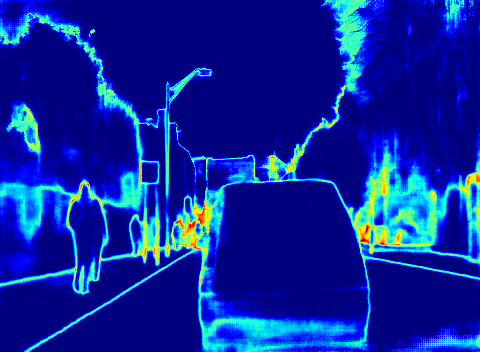
\includegraphics[width=\linewidth]{segnet_1_output_3.png}
        \vspace{1px}
		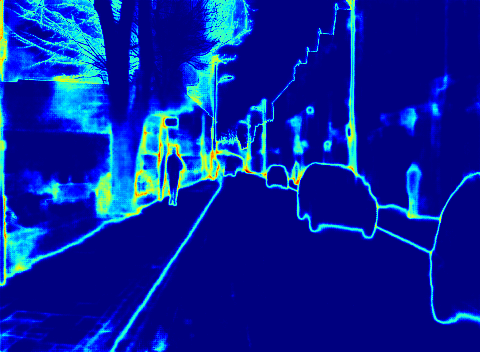
\includegraphics[width=\linewidth]{segnet_13_output_3.png}
        \vspace{1px}
        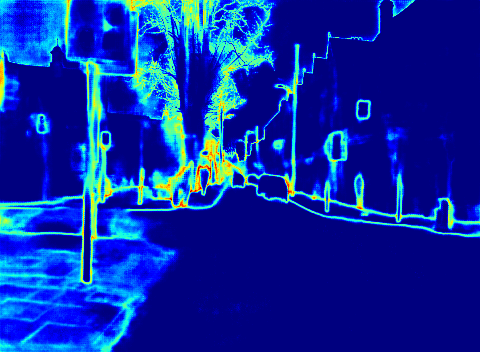
\includegraphics[width=\linewidth]{segnet_2_output_3.png}
        \caption{Aleatoric\\Uncertainty}
    \end{subfigure}
    \begin{subfigure}[t]{0.22\linewidth}
        \centering
		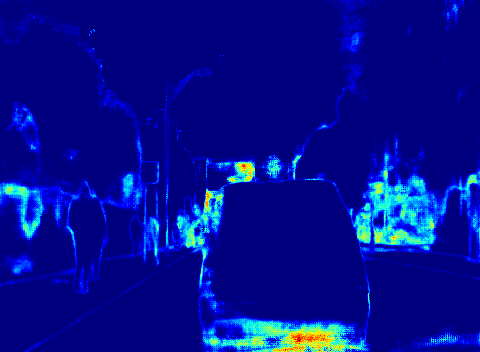
\includegraphics[width=\linewidth]{segnet_1_output_5.png}
        \vspace{1px}
		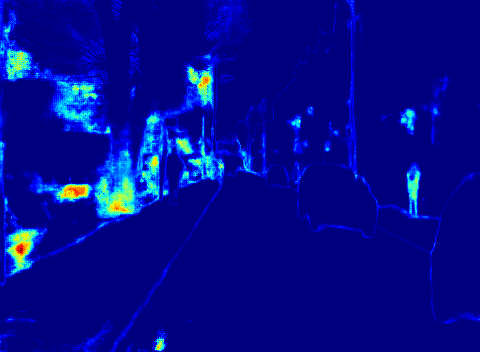
\includegraphics[width=\linewidth]{segnet_13_output_5.png}
        \vspace{1px}
        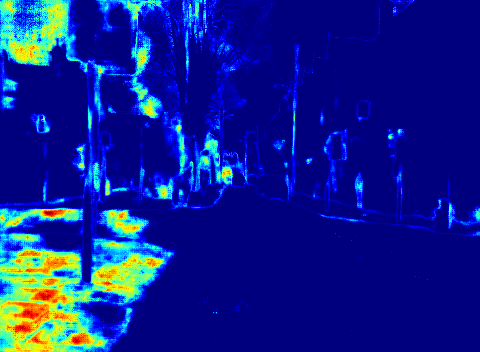
\includegraphics[width=\linewidth]{segnet_2_output_5.png}
        \caption{Epistemic\\Uncertainty}

\end{subfigure}}
\caption[Comparing different types of uncertainty in deep learning.]{\textbf{Illustrating the difference between aleatoric and epistemic uncertainty} for semantic segmentation on the CamVid dataset \citep{brostow2009semantic}. We observe aleatoric uncertainty captures object boundaries where labels are noisy. The bottom row shows a failure case of the segmentation model, when the model fails to segment the footpath, and the corresponding increased epistemic uncertainty.}
\label{fig:camvid_qual}
\end{figure*}

\subsection{Bayesian Deep Learning}
\label{related_work}

Existing approaches to Bayesian deep learning capture either epistemic uncertainty alone, or aleatoric uncertainty alone \citep{gal2016thesis}. These uncertainties are formalised as probability distributions over either the model parameters, or model outputs, respectively. Epistemic uncertainty is modelled by placing a prior distribution over a model's weights, and then trying to capture how much these weights vary given some data. Aleatoric uncertainty on the other hand is modelled by placing a distribution over the output of the model. For example, in regression our outputs might be modelled as corrupted with Gaussian random noise. In this case we are interested in learning the noise's variance as a function of different inputs (such noise can also be modelled with a constant value for all data points, but this is of less practical interest). These uncertainties, in the context of Bayesian deep learning, are explained in more detail in this section. 

\subsection{Epistemic Uncertainty in Bayesian Deep Learning}
\label{sect:dropout_VI}

To capture epistemic uncertainty in a neural network (NN) we put a prior distribution over its weights, for example a Gaussian prior distribution:
$\W \sim \N(0, I)$.

Such a model is referred to as a Bayesian neural network (BNN) \citep{ denker1991transforming, mackay1992practical, neal1995bayesian}. 
Bayesian neural networks replace the deterministic network's weight parameters with distributions over these parameters, and instead of optimising the network weights directly we average over all possible weights (referred to as \textit{marginalisation}). 
% (or optimise the parameters of the distributions (or integrate ) instead of .
Denoting the random output of the BNN as $\f^\W(\x)$, we define the model likelihood $p(\y | \f^\W(\x))$.
Given a dataset $\X=\{\x_1, ..., \x_N\}$, with labels $\Y=\{\y_1, ..., \y_N\}$, Bayesian inference is used to compute the posterior over the weights $p(\W | \X, \Y)$. This posterior captures the set of plausible model parameters, given the data.

For regression tasks we often define our likelihood as a Gaussian with mean given by the model output:
$
p(\y | \f^\W(\x)) = \N(\f^\W(\x), \sigma^2)
$,
with an observation noise scalar $\sigma$. 
For classification, on the other hand, we often squash the model output through a softmax function, and sample from the resulting probability vector:
% \newcommand{\softmax}{\text{softmax}}
$
p(\y | \f^\W(\x)) = \softmax(\f^\W(\x))
$.

BNNs are easy to formulate, but difficult to perform inference in. This is because the marginal probability $p(\Y | \X)$, required to evaluate the posterior, cannot be evaluated analytically. Different approximations exist \citep{graves2011practical, blundell2015weight, hernandez2016black, Gal2016Bayesian}.
In these approximate inference techniques, the posterior $p(\W | \X, \Y)$ is fitted with a simple distribution $q_\theta^*(\W)$, parametrised by $\theta$. This replaces the intractable problem of averaging over all weights in the BNN with an optimisation task, where we seek to optimise over the \textit{parameters of the simple distribution} instead of optimising the original neural network's parameters.

Dropout variational inference is a practical approach for approximate inference in large and complex models \citep{Gal2016Bayesian}. 
This inference is done by training a model with dropout before every weight layer, and by also performing dropout at test time to sample from the approximate posterior (stochastic forward passes, referred to as Monte Carlo dropout).
More formally, this approach is equivalent to performing approximate variational inference where we find a simple distribution $q_\theta^*(\W)$ in a tractable family which minimises the Kullback-Leibler (KL) divergence to the true model posterior $p(\W | \X, \Y)$. 
Dropout can be interpreted as a variational Bayesian approximation, where the approximating distribution is a mixture of two Gaussians with small variances and the mean of one of the Gaussians is fixed at zero. 
%
%The minimisation objective is given by \citep{jordan1999introduction}:
%% \newcommand{\cL}{\mathcal{L}}
%\begin{equation}  
%\cL(\theta, p) = - \frac{1}{N} \sum_{i=1}^N \log p(\y_i | \f^{\Wh_i}(\x_i)) + \frac{1 - p}{2N} ||\theta||^2
%\end{equation}
%with $N$ data points, dropout probability $p$, samples $\Wh_i \sim q_\theta^*(\W)$, and $\theta$ the set of the simple distribution's parameters to be optimised (weight matrices in dropout's case). In regression, for example, the negative log likelihood can be further simplified as
%\begin{equation}
%-\log p(\y_i | \f^{\Wh_i}(\x_i)) \propto  \frac{1}{2 \sigma^2}||\y_i - \f^{\Wh_i}(\x_i)||^2 + \frac{1}{2} \log \sigma^2
%\end{equation}
%for a Gaussian likelihood,
%% or 
%% \begin{align*}
%% -\log p(\y_i | \f^{\Wh_i}(\x_i)) \propto \frac{1}{\sigma^2}||\y_i - \f^{\Wh_i}(\x_i)|| + \log \sigma^2 
%% \end{align*}
%% for a Laplace likelihood,
%with $\sigma$ the model's observation noise parameter -- capturing how much noise we have in the outputs.

Epistemic uncertainty in the weights can be reduced by observing more data. This uncertainty induces prediction uncertainty by marginalising over the (approximate) weights posterior distribution. For classification this can be approximated using Monte Carlo integration as follows:
\begin{equation}
p(y=c | \x, \X, \Y) 
% &= \int p(y=c | \x, \W) p(\W | \X, \Y) \td \W \\
% &\approx 
% \int p(y=c | \x, \W) q_\theta^*(\W) \td \W \\
% &\approx 
% \frac{1}{T} \sum_{t=1}^T p(y=c | \x, \Wh_t) \\
% &=
\approx
\frac{1}{T} \sum_{t=1}^T \softmax(\f^{\Wh_t}(\x))
\end{equation}
with $T$ sampled masked model weights $\Wh_t \sim q_\theta^*(\W)$, where $q_\theta(\W)$ is the Dropout distribution \citep{gal2016thesis}. 
The uncertainty of this probability vector $\p$ can then be summarised using the entropy of the probability vector:
$H(\p) = - \sum_{c=1}^C p_c \log p_c.$
For regression this epistemic uncertainty is captured by the predictive variance, which can be approximated as:
\begin{equation}
\text{Var}(\y) \approx \sigma^2 + \frac{1}{T} \sum_{t=1}^T \f^{\Wh_t}(\x)^T \f^{\Wh_t}(\x_t) - E(\y)^T E(\y)
\end{equation}
with predictions in this epistemic model done by approximating the predictive mean: 
$E(\y) \approx \frac{1}{T} \sum_{t=1}^T \f^{\Wh_t}(\x).$
The first term in the predictive variance, $\sigma^2$, corresponds to the amount of noise inherent in the data (heteroscedastic noise -- which will be explained in more detail soon). The second part of the predictive variance measures how much the model is uncertain about its predictions -- this term will vanish when we have zero parameter uncertainty (i.e.\ when all draws $\Wh_t$ take the same constant value). 

\subsection{Heteroscedastic Aleatoric Uncertainty}
\label{sect:hetero}

In the previous section we captured model uncertainty -- uncertainty over the model parameters -- by approximating the distribution $p(\W | \X, \Y)$. To capture aleatoric uncertainty in regression, we would have to tune the observation noise parameter $\sigma$.

Homoscedastic regression assumes constant observation noise $\sigma$ for every input point $\x$. Heteroscedastic regression, on the other hand, assumes that observation noise can vary with input $\x$ \citep{nix1994estimating, le2005heteroscedastic}. Heteroscedastic models are useful in cases where parts of the observation space might have higher noise levels than others.
In non-Bayesian neural networks, this observation noise parameter is often fixed as part of the model's weight decay, and ignored. However, when made data-dependent, it can be learned as a function of the data.

We derive loss functions for both Gaussian and Laplacian priors.
The probability density function for the Gaussian distribution is given by:
\begin{equation}
P(x) = \frac{1}{{\sigma \sqrt {2\pi } }}e^{{{ - \left( {x - \mu } \right)^2 } \mathord{\left/ {\vphantom {{ - \left( {x - \mu } \right)^2 } {2\sigma ^2 }}} \right. \kern-\nulldelimiterspace} {2\sigma ^2 }}}.
\end{equation}
We wish our neural network to learn to estimate the distribution function. To construct the optimisation objective we take the negative log likelihood of this distribution,
\begin{equation}
-\log p(\y_i | \x_i) \propto \frac{1}{2\sigma^2}||\y_i - \x_i||^2 + \frac{1}{2} \log \sigma^2.
\end{equation}
Similarly for the Laplacian distribution,
\begin{equation}
-\log p(\y_i | \x_i) \propto \frac{\sqrt{2}}{\sigma}||\y_i - \x_i|| + \log \sigma.
\end{equation}
We can see that using a Gaussian prior results in an L2 norm and a Laplacian prior results in an L1 norm to form the residuals. This choice can be informed by the task, often in vision models it is better to use a L1 norm as it is more robust to large, outlying residuals.
However, for now we consider the loss with a Gaussian distribution. We can formulate a loss to train our deep learning models (with a Gaussian distribution) by:
\begin{equation}
\cL_\text{NN}(\theta) = \frac{1}{N} \sum_{i=1}^N \frac{1}{2\sigma(\x_i)^2} ||\y_i - \f(\x_i)||^2 + \frac{1}{2} \log \sigma(\x_i)^2 %+ \lambda ||\theta||^2
% \cL(\theta, p) = \frac{1}{N} \sum_{i=1}^N \log \frac{1}{\sigma(\x_i)^2}||\y_i - \f^{\Wh_i}(\x_i)||^2 + \log \sigma(\x_i)^2 + \frac{1 - p}{N} ||\theta||^2.
\end{equation}
% \red{TODO: change Gaussian to Laplace likelihood}
with added weight decay parametrized by $\lambda$ (and similarly for $l_1$ loss).
Note that here, unlike the above, variational inference is \textit{not} performed over the weights, but instead we perform maximum a posteriori (MAP) inference -- finding a single value for the model parameters $\theta$. This approach \textit{does not} capture epistemic model uncertainty, as epistemic uncertainty is a property of the model and not of the data.

In the next section we will combine these two types of uncertainties together in a single model. We will see how heteroscedastic noise can be interpreted as model attenuation, and develop a complimentary approach for the classification case. %We will study how each uncertainty affects the models trained.


\subsection{Combining Aleatoric and Epistemic Uncertainty in One Model}
\label{sec:method}

In the previous section we described existing Bayesian deep learning techniques. In this section we present novel contributions which extend this existing literature. We develop models that will allow us to study the effects of modelling either aleatoric uncertainty alone, epistemic uncertainty alone, or modelling both uncertainties together in a single model. This is followed by an observation that aleatoric uncertainty in regression tasks can be interpreted as learned loss attenuation -- making the loss more robust to noisy data. We follow that by extending the ideas of heteroscedastic regression to classification tasks. This allows us to learn loss attenuation for classification tasks as well. %, and obtain improved aleatoric uncertainty estimates in classification.


We wish to capture both epistemic and aleatoric uncertainty in a vision model.
For this we turn the heteroscedastic neural network in \cref{sect:hetero} into a Bayesian neural network by placing a distribution over its weights, with our construction in this section developed specifically for the case of vision models\footnote{Although this construction can be generalised for any heteroscedastic neural network architecture.}.

We need to infer the posterior distribution for a BNN model $\f$ mapping an input image, $\x$, to a unary output, $\hat{\y} \in \mathbb{R}$, and a measure of aleatoric uncertainty given by variance, $\mathbf{\sigma}^2$. We approximate the posterior over the BNN with a dropout variational distribution using the tools of \cref{sect:dropout_VI}. 
As before, we draw model weights from the approximate posterior $\Wh \sim q(\W)$ to obtain a model output, this time composed of both predictive mean as well as predictive variance:
\begin{equation}
[\hat{\y}, \hat{\mathbf{\sigma}}^2] = \f^{\Wh}(\textbf{x})
\end{equation}
where $\f$ is a Bayesian convolutional neural network parametrised by model weights $\Wh$. We can use a single network to transform the input $\x$, with its head split to predict both $\hat{\y}$ as well as $\hat{\sigma}^2$.

% For regression tasks we train our network to learn a continuous valued function and predict the unaries $x_i \in \mathbb{R}$. 
We fix a Gaussian likelihood to model our aleatoric uncertainty.
This induces a minimisation objective given labelled output points $x$:
\begin{equation}
\cL_{BNN}(\theta) = \frac{1}{D} \sum_i \frac{1}{2} \hat{\sigma}^{-2}_i ||\y_i-\hat{\y}_i||^2 + \frac{1}{2} \log{\hat{\sigma}_i^2}
\end{equation}
where $D$ is the number of output pixels $\y_i$ corresponding to input image $\x$, indexed by $i$ (additionally, the loss includes weight decay which is omitted for brevity). For example, we may set $D=1$ for image-level regression tasks, or $D$ equal to the number of pixels for dense prediction tasks (predicting a unary corresponding to each input image pixel). $\hat{\sigma}^2_i$ is the BNN output for the predicted variance for pixel $i$.

This loss consists of two components; the residual regression obtained with a stochastic sample through the model -- making use of the uncertainty over the parameters  -- and an uncertainty regularization term. We do not need `uncertainty labels' to learn uncertainty. Rather, we only need to supervise the learning of the regression task. We learn the variance, $\sigma^2$, implicitly from the loss function. The second regularization term prevents the network from predicting infinite uncertainty (and therefore zero loss) for all data points.

In practice, we train the network to predict the log variance, $s_i := \log \hat{\sigma}_i^2$: 
\begin{equation}
\cL_{BNN}(\theta) = \frac{1}{D} \sum_i \frac{1}{2} \exp (-s_i) ||\y_i-\hat{\y}_i||^2 + \frac{1}{2} s_i.
\label{eqn:aleatoric_regression_loss}
\end{equation}
This is because it is more stable than regressing the variance, $\sigma^2$, as the loss avoids a potential division by zero. The exponential mapping also allows us to regress unconstrained scalar values, where $\exp(-s_i)$ is resolved to the positive domain giving valid values for variance.

% Following the notation of the previous section, the predictive uncertainty in this combined model can be approximated using:
% \begin{align*}
% \text{Var}(\y) &\approx \frac{1}{T} \sum_{t=1}^T \f^{\Wh_t}(\x)^T \f^{\Wh_t}(\x_t)
% - E(\y)^T E(\y) \\
% &\qquad + \frac{1}{T} \sum_{t=1}^T (\sigma^{\Wh_t}(\x))^2.
% \end{align*}
To summarize, the predictive uncertainty for pixel $\y$ in this combined model can be approximated using:
\begin{equation}
\text{Var}(\y) \approx \frac{1}{T} \sum_{t=1}^T \hat{\y}_{t}^2
- \bigg( \frac{1}{T} \sum_{t=1}^T \hat{\y}_{t} \bigg)^2 + \frac{1}{T} \sum_{t=1}^T \hat{\sigma}_{t}^2
\end{equation}
with $\{ \hat{\y}_{t}, \hat{\sigma}_{t}^2 \}_{t=1}^T$ a set of $T$ sampled outputs: $\hat{\y}_{t}, \hat{\sigma}_{t}^2 = \f^{\Wh_t}(\x)$ for randomly masked weights $\Wh_t \sim q(\W)$.


\subsection{Heteroscedastic Uncertainty as Learned Loss Attenuation}

We observe that allowing the network to predict uncertainty, allows it effectively to temper the residual loss by $\exp(-s_i)$, which depends on the data. This acts similarly to an intelligent robust regression function. It allows the network to adapt the residual's weighting, and even allows the network to learn to attenuate the effect from erroneous labels. This makes the model more robust to noisy data: inputs for which the model learned to predict high uncertainty will have a smaller effect on the loss.

The model is discouraged from predicting high uncertainty for all points -- in effect ignoring the data -- through the $\log \sigma^2$ term. Large uncertainty increases the contribution of this term, and in turn penalizes the model: The model \textit{can} learn to ignore the data -- but is penalised for that. The model is also discouraged from predicting very low uncertainty for points with high residual error, as low $\sigma^2$ will exaggerate the contribution of the residual and will penalize the model. It is important to stress that this learned attenuation is not an ad-hoc construction, but a consequence of the probabilistic interpretation of the model. 

This learned loss attenuation property of heteroscedastic neural networks in regression is a desirable effect for classification models as well. 
However, heteroscedastic neural networks in classification are peculiar models because technically any classification task has input-dependent uncertainty. Nevertheless, the ideas above can be extended from regression heteroscedastic networks to classification heteroscedastic networks, which we discuss in the next section.


\subsection{Heteroscedastic Uncertainty in Classification Tasks}

We extend the results above to classification models, allowing us to get the equivalent of the learned loss attenuation property in classification as well.
For this we adapt the standard classification model to marginalise over intermediate heteroscedastic regression uncertainty placed over the \textit{logit space}.
We therefore explicitly refer to our proposed model adaptation as a \textit{heteroscedastic} classification neural network.

For classification tasks our model predicts a vector of unaries $\f_i$ for each pixel $i$, which when passed through a softmax operation, forms a probability vector $\p_i$. We change the model by placing a Gaussian distribution over the unaries vector:
\begin{equation}
\begin{split}
\hat{\x}_i | \W \sim \N(\f^\W_i, (\sigma_i^\W)^2)
\\
\hat{\p}_i = \softmax(\hat{\x}_i).
\end{split}
\end{equation}
Here $\f^\W_i, \sigma_i^\W$ are the network outputs with parameters $\W$.
This vector $\f^\W_i$ is corrupted with Gaussian noise with variance $(\sigma_i^\W)^2$ (a diagonal matrix with one element for each logit value), and the corrupted vector is then squashed with the softmax function to obtain $\p_i$, the probability vector for pixel $i$.

Our expected log likelihood for this model is given by:
\begin{equation}
E_{\N(\hat{\x}_i; \f^\W_i, (\sigma_i^\W)^2)}[\log \hat{\p}_{i,c}]
\end{equation}
with $c$ the observed class for input $i$,
which gives us our loss function.
Ideally, we would want to analytically integrate out this Gaussian distribution, but no analytic solution is known.
We therefore approximate the objective through Monte Carlo integration, and sample unaries through the softmax function.
We note that this operation is extremely fast because we perform the computation once (passing inputs through the model to get logits). We only need to sample from the logits, which is a fraction of the network's compute, and therefore does not significantly increase the model's test time. 
We can rewrite the above and obtain the following numerically-stable stochastic loss:
\begin{equation}
\begin{split}
\hat{\x}_{i,t} &= \f^\W_i + \epsilon_t, \quad \epsilon_t \sim \mathcal{N}(0,\,(\sigma_i^\W)^2)
\\
\cL_x &= \frac{1}{T} \sum_{i,t} (- \hat{x}_{i,t,c} + \log \sum_{c'} \exp \hat{x}_{i,t,c'})
\end{split}
\label{eqn:aleatoric_classification_loss}
\end{equation}
with $x_{i,t,c'}$ the $c'$ element in the logit vector $\x_{i,t}$. 

This objective can be interpreted as learning loss attenuation, similarly to the regression case.
To understand this objective, we concentrate on a single pixel $i$ and reformulate the objective as $\sum_{t} \log \sum_{c'} \exp (\hat{x}_{t,c'} - \hat{x}_{t,c})$ with $c$ the observed class and $t$ Gaussian samples. We shall analyse what this objective behaves like for various settings.
When the model gives the observed class a high logit value $f_{c}$ (compared to the logit values of other classes) and a low noise value $\sigma_{c}$, this loss will be near zero -- the ideal case. When the model attempts to give the observed class a low logit value (for example if the label is noisy and $f_{c'}$ is the highest logit for some incorrect $c' \neq c$), there are two cases of interest. If the observed class logit has a low noise value, then the loss will be penalised by approximately $f_{c'} - f_{c}$\footnote{To see this, pull the term $f_{c'} - f_{c}$ out of the log-sum-exp; the corresponding exponent will now be $\exp(0)=1$, and since this was the largest exponent, the remaining exp terms in the sum will be near zero.}. However, if the model increases the noise value for this last case, then some noise samples will take a high value and the penalisation will be decreased from this last quantity. Lastly, the model is discouraged from increasing the noise when the observed class is given a high logit value. This is because large noise would lead some logit samples to take high negative values, and these samples will increase the loss.


We next assess the above ideas empirically.


\subsection{Experiments}
\label{sec:results}

In this section we evaluate our methods with pixel-wise depth regression and semantic segmentation. An analysis of these results is given in the following section. To show the robustness of our learned loss attenuation -- a side-effect of modelling uncertainty -- we present results on an array of popular datasets, CamVid \citep{brostow2009semantic}, Make3D \citep{saxena2009make3d}, and NYUv2 Depth \citep{silberman2012indoor}, where we advance state-of-the-art.


For the following experiments we use the DenseNet architecture \citep{huang2016densely} which has been adapted for dense prediction tasks by \citep{jegou2016one}. We use our own independent implementation of the architecture using TensorFlow \citep{abadi2016tensorflow} (which slightly outperforms the original authors' implementation on CamVid by 0.2\%, see Table \ref{camvid}). For all experiments we train with $224\times224$ crops of batch size 4, and then fine-tune on full-size images with a batch size of 1. We train with RMS-Prop with a constant learning rate of $0.001$ and weight decay $10^{-4}$.



We model the benefit of combining both epistemic uncertainty as well as aleatoric uncertainty using our developments presented in \cref{sec:method}. 

\subsubsection{Semantic Segmentation}

To demonstrate our method for semantic segmentation, we use two datasets, CamVid \citep{brostow2009semantic} and NYU v2 \citep{silberman2012indoor}. CamVid is a road scene understanding dataset and has been introduced in \cref{CamVid}. In Table \ref{camvid} we present results for our architecture. Our method sets a new state-of-the-art on this dataset with mean intersection over union (IoU) score of $67.5\%$. We observe that modelling both aleatoric and epistemic uncertainty improves over the baseline result.  The implicit attenuation obtained from the aleatoric loss provides a larger improvement than the epistemic uncertainty model. However, the combination of both uncertainties improves performance even further. This shows that for this application it is more important to model aleatoric uncertainty, suggesting that epistemic uncertainty can be mostly explained away in this large data setting.

Secondly, NYUv2 \citep{silberman2012indoor} is a challenging indoor segmentation dataset with 40 different semantic classes (similar to SUN RGB-D). It has 1449 images with resolution $640\times480$ from 464 different indoor scenes. Table \ref{nyuv2} shows our results. This dataset is much harder than CamVid because there is significantly less structure in indoor scenes compared to street scenes, and because of the increased number of semantic classes. We use DeepLabLargeFOV \citep{chen2016deeplab} as our baseline model. We improve baseline performance by giving the model flexibility to estimate uncertainty and attenuate the loss. The effect is more pronounced, perhaps because the dataset is more difficult. Additional qualitative results are given in \cref{fig:qual_camvid2}, \cref{fig:qual_sun} and \cref{fig:qual_pascal}.



\subsubsection{Pixel-wise Depth Regression}

We demonstrate the efficacy of our method for regression using two popular monocular depth regression datasets, Make3D \citep{saxena2009make3d} and NYUv2 Depth \citep{silberman2012indoor}. The Make3D dataset consists of 400 training and 134 testing images, gathered using a 3-D laser scanner. We evaluate our method using the same standard as \citep{laina2016deeper}, resizing images to $345\times460$ pixels and evaluating on pixels with depth less than $70m$. NYUv2 Depth is taken from the same dataset used for classification above. It contains RGB-D imagery from 464 different indoor scenes. We compare to previous approaches for Make3D in Table \ref{make3d} and NYUv2 Depth in Table \ref{nyuv2depth}, using standard metrics (for a description of these metrics please see \citep{eigen2014depth}).





\begin{table}
\begin{subtable}[b]{.47\textwidth}
\centering
\scalebox{0.85}{
\begin{tabular}{l|c}
    \toprule
\textbf{CamVid} & IoU \\
    \midrule
SegNet \citep{badrinarayanan2017segnet} & 46.4 \\
FCN-8 \citep{long2015fully} & 57.0 \\
chen2016deeplab-LFOV \citep{chen2016deeplab} & 61.6 \\
Bayesian SegNet \citep{kendall2015bayesian}  & 63.1 \\
Dilation8 \citep{YuKoltun2016} & 65.3 \\
Dilation8 + FSO \citep{kundu2016feature} & 66.1 \\
DenseNet \citep{jegou2016one} & 66.9 \\
    \midrule
\multicolumn{2}{c}{\textit{This work:}} \\
    \midrule
DenseNet  (Our Implementation) & 67.1 \\
+ Aleatoric Uncertainty & 67.4 \\
+ Epistemic Uncertainty & 67.2 \\
+ Aleatoric \& Epistemic & \textbf{67.5} \\
    \bottomrule
\end{tabular}}
\caption{CamVid dataset for road scene segmentation.}
\label{camvid}
\end{subtable}
\quad
\begin{subtable}[b]{.47\textwidth}
\centering
\scalebox{0.85}{
\begin{tabular}{p{4cm}|c|c}
    \toprule
\textbf{NYUv2 40-class} & Accuracy & IoU \\
    \midrule
\citet{gupta2014learning} & 60.3 & 28.6 \\
SegNet \citep{badrinarayanan2017segnet} & 66.1 & 23.6 \rule{0pt}{2.6ex} \\
FCN-8 \citep{long2015fully} & 61.8 & 31.6 \\
Bayesian SegNet \citep{kendall2015bayesian} & 68.0 & 32.4 \\
\citet{eigen2015predicting} & 65.6 & 34.1 \\
    \midrule
\multicolumn{3}{c}{\textit{This work:}} \\
    \midrule
chen2016deeplabLargeFOV & 70.1 & 36.5 \\
+ Aleatoric Uncertainty & 70.4 & 37.1 \\
+ Epistemic Uncertainty & 70.2 & 36.7 \\
+ Aleatoric \& Epistemic & \textbf{70.6} & \textbf{37.3} \\
    \bottomrule
\end{tabular}}
\caption{NYUv2 40-class dataset for indoor scenes.}
\label{nyuv2}
\end{subtable}
\caption[Probabilisitc semantic segmentation performance.]{\textbf{Semantic segmentation performance.} Modelling both aleatoric and epistemic uncertainty gives a notable improvement in segmentation accuracy over state of the art baselines.}
\end{table}


\begin{table}[p]
\begin{subtable}[b]{\textwidth}
\centering
\begin{tabular}{l|c|c|c}%|c|c|c}
    \toprule
\textbf{Make3D} & rel & rms & log$_{10}$ \\ 
    \midrule
\citet{karsch2012depth} & 0.355 & 9.20 & 0.127 \\ %& - & - & - \\
\citet{liu2014discrete} & 0.335 & 9.49 & 0.137 \\ %& - & - & - \\
\citep{liu2015deep} & 0.314 & 8.60 & 0.119 \\ %& - & - & - \\
\citet{li2015depth} & 0.278 & 7.19 & 0.092 \\ %& - & - & - \\
\citet{laina2016deeper} & 0.176 &  4.46 & 0.072 \\ 
    \midrule
\multicolumn{4}{c}{\textit{This work:}} \\ 
    \midrule
DenseNet Baseline & 0.167 & 3.92 & 0.064 \\ %& 82.7\% & 93.7\% & 97.5\% \\
+ Aleatoric Uncertainty & \textbf{0.149} & 3.93 & \textbf{0.061} \\ %& \textbf{83.7\%} & \textbf{93.9\%} & \textbf{97.6\%} \\
+ Epistemic Uncertainty & 0.162 & \textbf{3.87} & 0.064 \\ %& 82.6\% & 93.8\% & \textbf{97.6\%} \\
+ Aleatoric \& Epistemic & \textbf{0.149} & 4.08 & 0.063 \\ %& 83.1\% & 93.3\% & 97.0\% \\
    \bottomrule
\end{tabular}
\caption{Make3D depth dataset \citep{saxena2009make3d}.}
\label{make3d}
\end{subtable}


\begin{subtable}[b]{\textwidth}
\centering
\begin{tabular}{l|c|c|c|c|c|c}
    \toprule
\textbf{NYU v2 Depth}  & rel & rms & log$_{10}$ & $\delta_1$ & $\delta_2$ & $\delta_3$ \rule{0pt}{2.6ex} \\ 
    \midrule
\citet{karsch2012depth} & 0.374 & 1.12 & 0.134 & - & - & - \\
\citet{ladicky2014pulling} & - & - & - & 54.2\% & 82.9\% & 91.4\% \\
\citet{liu2014discrete} & 0.335 & 1.06 & 0.127 & - & - & - \\
\citet{li2015depth} & 0.232 & 0.821 & 0.094 & 62.1\% & 88.6\% & 96.8\% \\
\citet{liu2015deep} & 0.230 & 0.824 & 0.095 & 61.4\% & 88.3\% & 97.1\% \\
\citet{eigen2014depth} & 0.215 & 0.907 & - & 61.1\% & 88.7\% & 97.1\% \\
\citet{eigen2015predicting} & 0.158 & 0.641 & - & 76.9\% & 95.0\% & 98.8\% \\
\citet{laina2016deeper} & 0.127 & 0.573 & 0.055 & 81.1\% & 95.3\% & 98.8\% \\ 
    \midrule
\multicolumn{7}{c}{\textit{This work:}} \\ 
    \midrule
DenseNet Baseline & 0.117 & 0.517 & 0.051 & 80.2\% & 95.1\% & 98.8\% \\
+ Aleatoric Uncertainty & 0.112 & 0.508 & 0.046 & 81.6\% & 95.8\% & 98.8\% \\
+ Epistemic Uncertainty & 0.114 & 0.512 & 0.049 & 81.1\% & 95.4\% & 98.8\% \\
+ Aleatoric \& Epistemic & \textbf{0.110} & \textbf{0.506} & \textbf{0.045} & \textbf{81.7\%} & \textbf{95.9\%} & \textbf{98.9\%} \\
    \bottomrule
\end{tabular}
\caption{NYUv2 depth dataset \citep{silberman2012indoor}.}
\label{nyuv2depth}
\end{subtable}
\caption[Probabilistic monocular depth regression performance.]{\textbf{Monocular depth regression performance.} Comparison to previous approaches on depth regression dataset NYUv2 Depth. Modelling the combination of uncertainties improves accuracy.}
\end{table}



These results show that aleatoric uncertainty is able to capture many aspects of this task which are inherently difficult. For example, in the qualitative results in Figure \ref{fig:nyud_qual} and \ref{fig:make3d_qual} we observe that aleatoric uncertainty is greater for large depths, reflective surfaces and occlusion boundaries in the image. These are common failure modes of monocular depth algorithms \citep{laina2016deeper}. On the other hand, these qualitative results show that epistemic uncertainty captures difficulties due to lack of data. For example, we observe larger uncertainty for objects which are rare in the training set such as humans in the third example of Figure \ref{fig:nyud_qual}.




In summary, we have demonstrated that our model can improve performance over non-Bayesian baselines by implicitly learning attenuation of systematic noise and difficult concepts. For example we observe high aleatoric uncertainty for distant objects and on object and occlusion boundaries.

\subsection{What Do Aleatoric and Epistemic Uncertainties Capture?}

In \cref{sec:results} we showed that modelling aleatoric and epistemic uncertainties improves prediction performance, with the combination performing even better.
In this section we wish to study the effectiveness of modelling aleatoric and epistemic uncertainty. In particular, we wish to quantify the performance of these uncertainty measurements and analyse what they capture.

\begin{figure}[p]
\vspace{-5mm}
\begin{center}
\resizebox{0.85\linewidth}{!}{
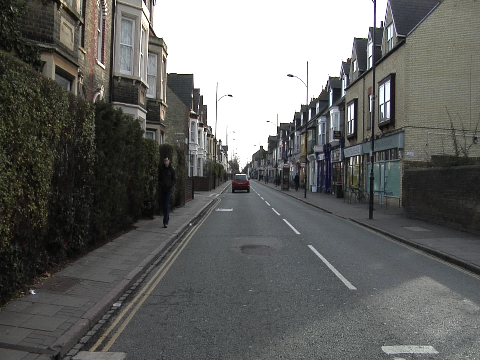
\includegraphics[height=0.125\linewidth]{BayesianSegNet/segnet_bayes_00016_input.png}
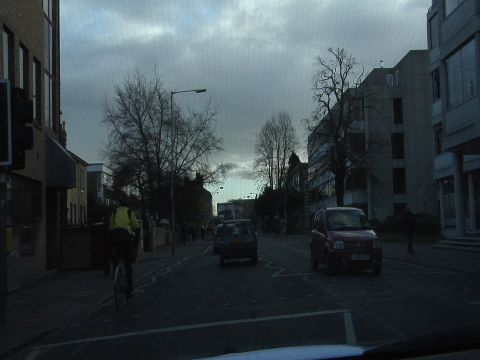
\includegraphics[height=0.125\linewidth]{BayesianSegNet/segnet_bayes_00172_input.png}
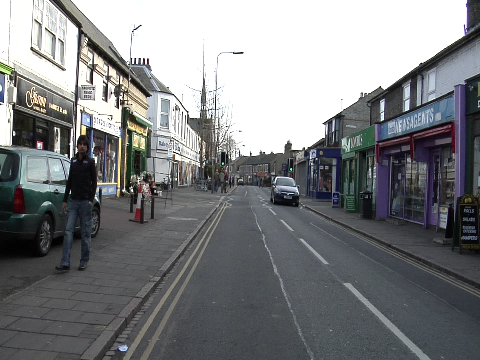
\includegraphics[height=0.125\linewidth]{BayesianSegNet/segnet_bayes_00145_input.png}
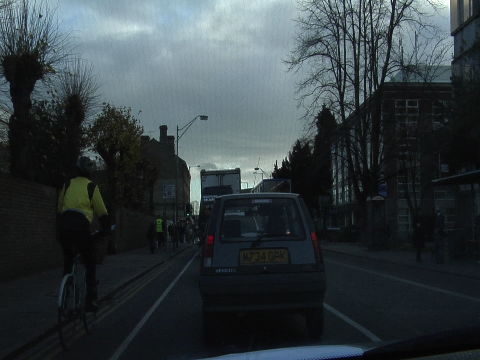
\includegraphics[height=0.125\linewidth]{BayesianSegNet/segnet_bayes_00183_input.png}
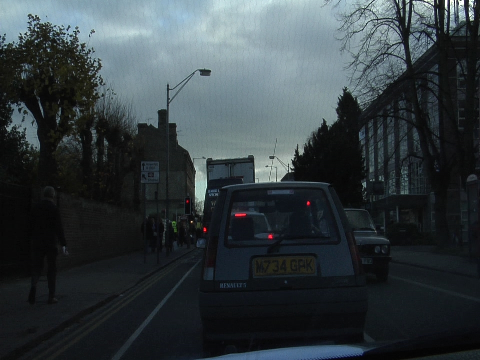
\includegraphics[height=0.125\linewidth]{BayesianSegNet/segnet_bayes_00193_input.png}
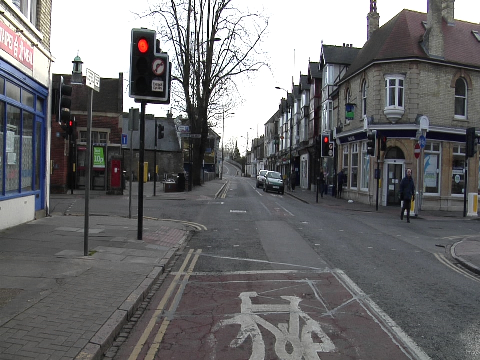
\includegraphics[height=0.125\linewidth]{BayesianSegNet/segnet_bayes_00083_input.png}
}
\resizebox{0.85\linewidth}{!}{
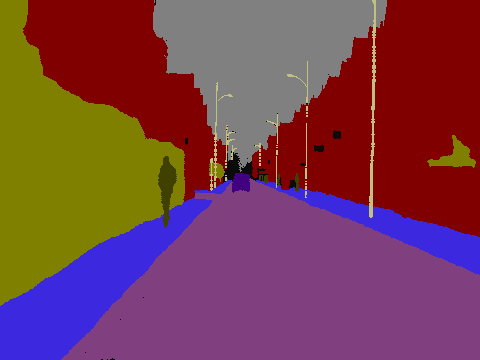
\includegraphics[height=0.125\linewidth]{BayesianSegNet/segnet_bayes_00016_gt.png}
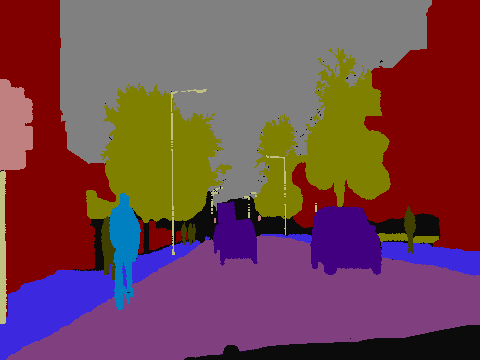
\includegraphics[height=0.125\linewidth]{BayesianSegNet/segnet_bayes_00172_gt.png}
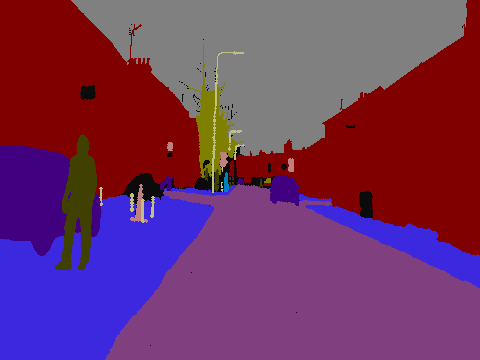
\includegraphics[height=0.125\linewidth]{BayesianSegNet/segnet_bayes_00145_gt.png}
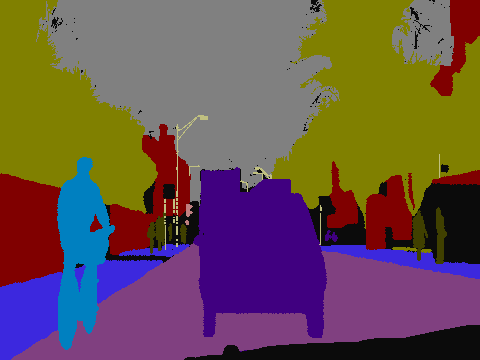
\includegraphics[height=0.125\linewidth]{BayesianSegNet/segnet_bayes_00183_gt.png}
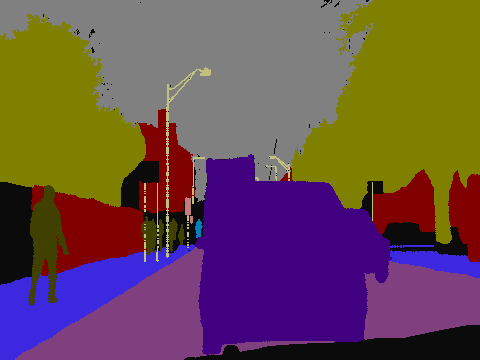
\includegraphics[height=0.125\linewidth]{BayesianSegNet/segnet_bayes_00193_gt.png}
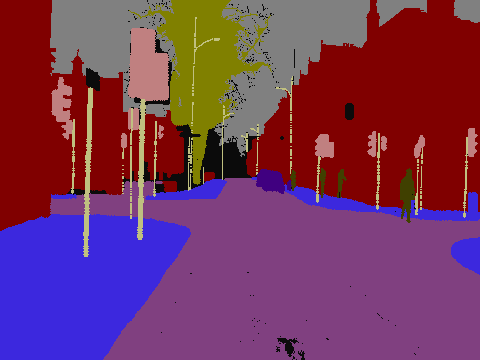
\includegraphics[height=0.125\linewidth]{BayesianSegNet/segnet_bayes_00083_gt.png}
}
\resizebox{0.85\linewidth}{!}{
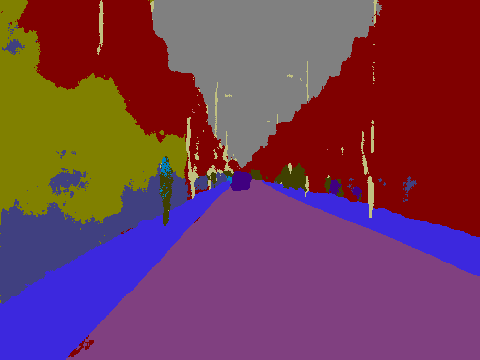
\includegraphics[height=0.125\linewidth]{BayesianSegNet/segnet_bayes_00016_segmentation.png}
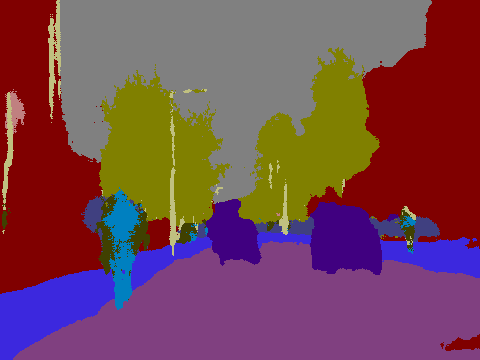
\includegraphics[height=0.125\linewidth]{BayesianSegNet/segnet_bayes_00172_segmentation.png}
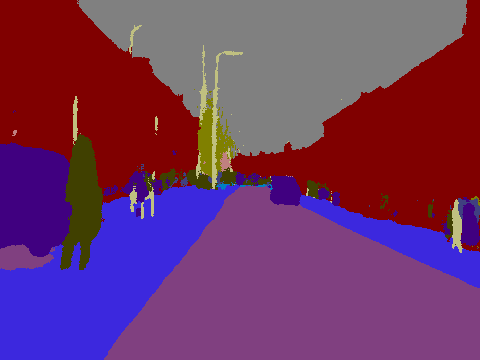
\includegraphics[height=0.125\linewidth]{BayesianSegNet/segnet_bayes_00145_segmentation.png}
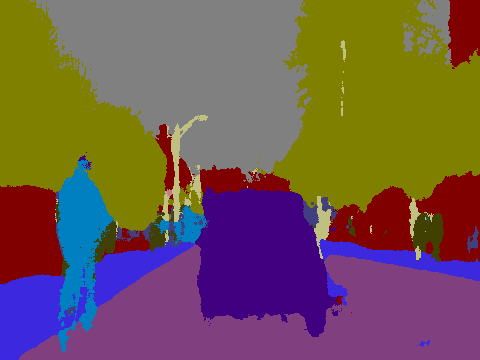
\includegraphics[height=0.125\linewidth]{BayesianSegNet/segnet_bayes_00183_segmentation.png}
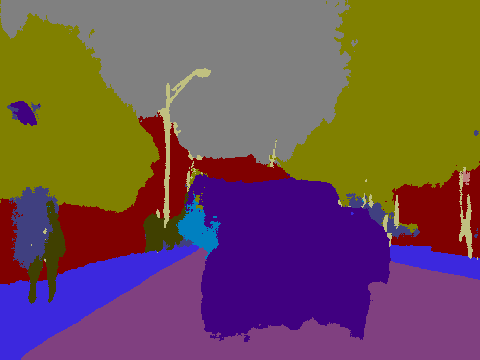
\includegraphics[height=0.125\linewidth]{BayesianSegNet/segnet_bayes_00193_segmentation.png}
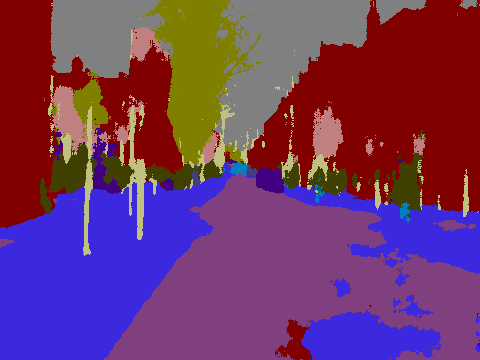
\includegraphics[height=0.125\linewidth]{BayesianSegNet/segnet_bayes_00083_segmentation.png}
}
\resizebox{0.85\linewidth}{!}{
\includegraphics[height=0.125\linewidth]{BayesianSegNet/segnet_bayes_00016_uncertainty.png}
\includegraphics[height=0.125\linewidth]{BayesianSegNet/segnet_bayes_00172_uncertainty.png}
\includegraphics[height=0.125\linewidth]{BayesianSegNet/segnet_bayes_00145_uncertainty.png}
\includegraphics[height=0.125\linewidth]{BayesianSegNet/segnet_bayes_00183_uncertainty.png}
\includegraphics[height=0.125\linewidth]{BayesianSegNet/segnet_bayes_00193_uncertainty.png}
\includegraphics[height=0.125\linewidth]{BayesianSegNet/segnet_bayes_00083_uncertainty.png}
}
\end{center}
\caption[Bayesian SegNet results on the CamVid dataset.]{\footnotesize\textbf{Bayesian SegNet results on CamVid dataset.} From top: input image, ground truth, Bayesian SegNet's segmentation prediction, and overall model uncertainty averaged across all classes.
   }
\label{fig:qual_camvid2}

\begin{center}
\resizebox{0.85\linewidth}{!}{
\includegraphics[height=0.125\linewidth]{BayesianSegNet/segnet_bayes_00244_input.png}
\includegraphics[height=0.125\linewidth]{BayesianSegNet/segnet_bayes_00309_input.png}
\includegraphics[height=0.125\linewidth]{BayesianSegNet/segnet_bayes_00414_input.png}
\includegraphics[height=0.125\linewidth]{BayesianSegNet/segnet_bayes_00375_input.png}
\includegraphics[height=0.125\linewidth]{BayesianSegNet/segnet_bayes_00461_input.png}
\includegraphics[height=0.125\linewidth]{BayesianSegNet/segnet_bayes_00116_input.png}
\includegraphics[height=0.125\linewidth]{BayesianSegNet/segnet_bayes_01035_input.png}
\includegraphics[height=0.125\linewidth]{BayesianSegNet/segnet_bayes_00856_input.png}
}
\resizebox{0.85\linewidth}{!}{
\includegraphics[height=0.125\linewidth]{BayesianSegNet/segnet_bayes_00244_gt.png}
\includegraphics[height=0.125\linewidth]{BayesianSegNet/segnet_bayes_00309_gt.png}
\includegraphics[height=0.125\linewidth]{BayesianSegNet/segnet_bayes_00414_gt.png}
\includegraphics[height=0.125\linewidth]{BayesianSegNet/segnet_bayes_00375_gt.png}
\includegraphics[height=0.125\linewidth]{BayesianSegNet/segnet_bayes_00461_gt.png}
\includegraphics[height=0.125\linewidth]{BayesianSegNet/segnet_bayes_00116_gt.png}
\includegraphics[height=0.125\linewidth]{BayesianSegNet/segnet_bayes_01035_gt.png}
\includegraphics[height=0.125\linewidth]{BayesianSegNet/segnet_bayes_00856_gt.png}
}
\resizebox{0.85\linewidth}{!}{
\includegraphics[height=0.125\linewidth]{BayesianSegNet/segnet_bayes_00244_segmentation.png}
\includegraphics[height=0.125\linewidth]{BayesianSegNet/segnet_bayes_00309_segmentation.png}
\includegraphics[height=0.125\linewidth]{BayesianSegNet/segnet_bayes_00414_segmentation.png}
\includegraphics[height=0.125\linewidth]{BayesianSegNet/segnet_bayes_00375_segmentation.png}
\includegraphics[height=0.125\linewidth]{BayesianSegNet/segnet_bayes_00461_segmentation.png}
\includegraphics[height=0.125\linewidth]{BayesianSegNet/segnet_bayes_00116_segmentation.png}
\includegraphics[height=0.125\linewidth]{BayesianSegNet/segnet_bayes_01035_segmentation.png}
\includegraphics[height=0.125\linewidth]{BayesianSegNet/segnet_bayes_00856_segmentation.png}
}
\resizebox{0.85\linewidth}{!}{
\includegraphics[height=0.125\linewidth]{BayesianSegNet/segnet_bayes_00244_uncertainty.png}
\includegraphics[height=0.125\linewidth]{BayesianSegNet/segnet_bayes_00309_uncertainty.png}
\includegraphics[height=0.125\linewidth]{BayesianSegNet/segnet_bayes_00414_uncertainty.png}
\includegraphics[height=0.125\linewidth]{BayesianSegNet/segnet_bayes_00375_uncertainty.png}
\includegraphics[height=0.125\linewidth]{BayesianSegNet/segnet_bayes_00461_uncertainty.png}
\includegraphics[height=0.125\linewidth]{BayesianSegNet/segnet_bayes_00116_uncertainty.png}
\includegraphics[height=0.125\linewidth]{BayesianSegNet/segnet_bayes_01035_uncertainty.png}
\includegraphics[height=0.125\linewidth]{BayesianSegNet/segnet_bayes_00856_uncertainty.png}
}
\end{center}
\caption[Bayesian SegNet results on the SUN RGB-D dataset.]{\footnotesize \textbf{Bayesian SegNet results on the SUN RGB-D dataset.} From top: input image, ground truth, Bayesian SegNet's segmentation prediction, and overall model uncertainty averaged across all classes.}
\label{fig:qual_sun}

\begin{center}
\resizebox{0.85\linewidth}{!}{
\includegraphics[height=0.125\linewidth]{BayesianSegNet/segnet_bayes_00005_input.png}
\includegraphics[height=0.125\linewidth]{BayesianSegNet/segnet_bayes_00052_input.png}
\includegraphics[height=0.125\linewidth]{BayesianSegNet/segnet_bayes_00202_input.png}
\includegraphics[height=0.125\linewidth]{BayesianSegNet/segnet_bayes_00147_input.png}
\includegraphics[height=0.125\linewidth]{BayesianSegNet/segnet_bayes_00148_input.png}
\includegraphics[height=0.125\linewidth]{BayesianSegNet/segnet_bayes_00166_input.png}
\includegraphics[height=0.125\linewidth]{BayesianSegNet/segnet_bayes_00017_input.png}
\includegraphics[height=0.125\linewidth]{BayesianSegNet/segnet_bayes_00023_input.png}
}
\resizebox{0.85\linewidth}{!}{
\includegraphics[height=0.125\linewidth]{BayesianSegNet/segnet_bayes_00005_segmentation.png}
\includegraphics[height=0.125\linewidth]{BayesianSegNet/segnet_bayes_00052_segmentation.png}
\includegraphics[height=0.125\linewidth]{BayesianSegNet/segnet_bayes_00202_segmentation.png}
\includegraphics[height=0.125\linewidth]{BayesianSegNet/segnet_bayes_00147_segmentation.png}
\includegraphics[height=0.125\linewidth]{BayesianSegNet/segnet_bayes_00148_segmentation.png}
\includegraphics[height=0.125\linewidth]{BayesianSegNet/segnet_bayes_00166_segmentation.png}
\includegraphics[height=0.125\linewidth]{BayesianSegNet/segnet_bayes_00017_segmentation.png}
\includegraphics[height=0.125\linewidth]{BayesianSegNet/segnet_bayes_00023_segmentation.png}
}
\resizebox{0.85\linewidth}{!}{
\includegraphics[height=0.125\linewidth]{BayesianSegNet/segnet_bayes_00005_uncertainty.png}
\includegraphics[height=0.125\linewidth]{BayesianSegNet/segnet_bayes_00052_uncertainty.png}
\includegraphics[height=0.125\linewidth]{BayesianSegNet/segnet_bayes_00202_uncertainty.png}
\includegraphics[height=0.125\linewidth]{BayesianSegNet/segnet_bayes_00147_uncertainty.png}
\includegraphics[height=0.125\linewidth]{BayesianSegNet/segnet_bayes_00148_uncertainty.png}
\includegraphics[height=0.125\linewidth]{BayesianSegNet/segnet_bayes_00166_uncertainty.png}
\includegraphics[height=0.125\linewidth]{BayesianSegNet/segnet_bayes_00017_uncertainty.png}
\includegraphics[height=0.125\linewidth]{BayesianSegNet/segnet_bayes_00023_uncertainty.png}
}
\end{center}
\caption[Bayesian SegNet results on the Pascal VOC dataset.]{\footnotesize \textbf{Pascal VOC 2012 dataset.} From top: input image, Bayesian SegNet's segmentation prediction, and overall model uncertainty averaged across all classes. Ground truth segmentation not available for Pascal test images.}
\label{fig:qual_pascal}
\end{figure}
% \begin{figure}[h!]
% \centering
% \resizebox{\linewidth}{!}{
% \includegraphics[width=0.18\linewidth]{segnet_5_output_0.png}
% \includegraphics[width=0.18\linewidth]{segnet_5_output_2.png}
% \includegraphics[width=0.18\linewidth]{segnet_5_output_1.png}
% \includegraphics[width=0.18\linewidth]{segnet_5_output_3.png}
% \includegraphics[width=0.18\linewidth]{segnet_5_output_4.png}}
% \caption[NYUv2 40-Class segmentation.]{NYUv2 40-Class segmentation. From top-left: input image, ground truth, segmentation, aleatoric and epistemic uncertainty.}
% \label{fig:nyu_qual}
% \end{figure}

\begin{figure*}[p]
\centering
\resizebox{\linewidth}{!}{
\includegraphics[width=0.3\linewidth,trim={40 10 40 60},clip]{segnet_55_output_0.png}
\includegraphics[width=0.3\linewidth,trim={40 10 40 60},clip]{segnet_55_output_1.png}
\includegraphics[width=0.3\linewidth,trim={40 10 40 60},clip]{segnet_55_output_2.png}
\includegraphics[width=0.3\linewidth,trim={40 10 40 60},clip]{segnet_55_output_3.png}
\includegraphics[width=0.3\linewidth]{segnet_55_output_4.png}}
~
\resizebox{\linewidth}{!}{
\includegraphics[width=0.3\linewidth,trim={40 10 40 60},clip]{segnet_60_output_0.png}
\includegraphics[width=0.3\linewidth,trim={40 10 40 60},clip]{segnet_60_output_1.png}
\includegraphics[width=0.3\linewidth,trim={40 10 40 60},clip]{segnet_60_output_2.png}
\includegraphics[width=0.3\linewidth,trim={40 10 40 60},clip]{segnet_60_output_3.png}
\includegraphics[width=0.3\linewidth]{segnet_60_output_4.png}}
~
\resizebox{\linewidth}{!}{
\includegraphics[width=0.3\linewidth,trim={40 10 40 60},clip]{segnet_139_output_0.png}
\includegraphics[width=0.3\linewidth,trim={40 10 40 60},clip]{segnet_139_output_1.png}
\includegraphics[width=0.3\linewidth,trim={40 10 40 60},clip]{segnet_139_output_2.png}
\includegraphics[width=0.3\linewidth,trim={40 10 40 60},clip]{segnet_139_output_3.png}
\includegraphics[width=0.3\linewidth]{segnet_139_output_4.png}}
\caption[NYUv2 Depth results.]{NYUv2 Depth results. From left: input image, ground truth, depth regression, aleatoric uncertainty, and epistemic uncertainty.}
\label{fig:nyud_qual}
% \end{figure*}

% \begin{figure*}[h]
\centering
\resizebox{\linewidth}{!}{
\includegraphics[width=0.3\linewidth]{segnet_125_output_0.png}
\includegraphics[width=0.3\linewidth]{segnet_125_output_1.png}
\includegraphics[width=0.3\linewidth]{segnet_125_output_2.png}
\includegraphics[width=0.3\linewidth]{segnet_125_output_3.png}
\includegraphics[width=0.3\linewidth]{segnet_125_output_4.png}}
~
\resizebox{\linewidth}{!}{
\includegraphics[width=0.3\linewidth]{segnet_117_output_0.png}
\includegraphics[width=0.3\linewidth]{segnet_117_output_1.png}
\includegraphics[width=0.3\linewidth]{segnet_117_output_2.png}
\includegraphics[width=0.3\linewidth]{segnet_117_output_3.png}
\includegraphics[width=0.3\linewidth]{segnet_117_output_4.png}}
~
% \resizebox{\linewidth}{!}{
% \includegraphics[width=0.3\linewidth]{segnet_111_output_0.png}
% \includegraphics[width=0.3\linewidth]{segnet_111_output_1.png}
% \includegraphics[width=0.3\linewidth]{segnet_111_output_2.png}
% \includegraphics[width=0.3\linewidth]{segnet_111_output_3.png}
% \includegraphics[width=0.3\linewidth]{segnet_111_output_4.png}}
% ~
\resizebox{\linewidth}{!}{
\includegraphics[width=0.3\linewidth]{segnet_11_output_0.png}
\includegraphics[width=0.3\linewidth]{segnet_11_output_1.png}
\includegraphics[width=0.3\linewidth]{segnet_11_output_2.png}
\includegraphics[width=0.3\linewidth]{segnet_11_output_3.png}
\includegraphics[width=0.3\linewidth]{segnet_11_output_4.png}}
\caption[Qualitative results on the Make3D depth regression dataset.]{Qualitative results on the Make3D depth regression dataset. Left to right: input image, ground truth, depth prediction, aleatoric uncertainty, epistemic uncertainty. 
% Make3D does not provide labels for depth greater than 70m, therefore these distances dominate the epistemic uncertainty signal. Aleatoric uncertainty is prevalent around depth edges or distant points.
}
\label{fig:make3d_qual}
\end{figure*}


\subsubsection{Qualitative observations}
\fig{qual_camvid2} shows segmentations and model uncertainty results from Bayesian SegNet (SegNet evaluated with Monte Carlo dropout \citep{kendall2015bayesian}) on CamVid Road Scenes \citep{brostow2009semantic}. \cref{fig:qual_sun} shows SUN RGB-D Indoor Scene Understanding \citep{song2015sun} results and \cref{fig:qual_pascal} has Pascal VOC \citep{pascal} results. These figures show the qualitative performance of Bayesian SegNet. We observe that segmentation predictions are smooth, with a sharp segmentation around object boundaries. Also, when the model predicts an incorrect label, the model uncertainty is generally very high. More generally, we observe that a high model uncertainty is predominantly caused by three situations.

Firstly, at class boundaries the model often displays a high level of uncertainty. This reflects the ambiguity surrounding the definition of defining where these labels transition. The Pascal results clearly illustrate this in \cref{fig:qual_pascal}.

Secondly, objects which are visually difficult to identify often appear uncertain to the model. This is often the case when objects are occluded or at a distance from the camera.

The third situation causing model uncertainty is when the object appears visually ambiguous to the model. As an example, cyclists in the CamVid results (\cref{fig:qual_camvid2}) are visually similar to pedestrians, and the model often displays uncertainty around them. We observe similar results with visually similar classes in SUN (\cref{fig:qual_sun}) such as chair and sofa, or bench and table. In Pascal this is often observed between cat and dog, or train and bus classes.

\begin{figure}[t]
    \centering
    \begin{subfigure}[t]{0.45\linewidth}
        \centering
        \includegraphics[width=\linewidth]{scatter_camvid.eps}
        \caption{Performance vs. mean\\model uncertainty}
        \label{fig:unc_acc2}
    \end{subfigure}
    \begin{subfigure}[t]{0.45\linewidth}
        \centering
        \includegraphics[width=\linewidth]{scatter_camvid_freq.eps}
        \centering\caption{Class frequency vs. mean\\model uncertainty}
        \label{fig:unc_freq2}
    \end{subfigure}
	\caption[Analysis of Bayesian SegNet's model uncertainty.]{\textbf{Bayesian SegNet performance and frequency compared to mean model uncertainty} for each class in CamVid road scene understanding dataset. These figures show a strong inverse relationships. We observe in (a) that the model is more confident with accurate classes. (b) shows classes that Bayesian SegNet is confident at are more prevalent in the dataset. Conversely, for the rare classes such as Sign Symbol and Bicyclist, Bayesian SegNet has a much higher model uncertainty.}
\end{figure}

\subsubsection{Quality of Uncertainty Metric}

To understand what causes the model to be uncertain, we have plotted the relationship between uncertainty and accuracy in \cref{fig:unc_acc2} and between uncertainty and the frequency of each class in the dataset in \cref{fig:unc_freq2}. Uncertainty is calculated as the mean uncertainty value for each pixel of that class in a test dataset. We observe an inverse relationship between uncertainty and class accuracy or class frequency. This shows that the model is more confident about classes which are easier or occur more often, and less certain about rare and challenging classes.

In \cref{sec:results} we showed that modelling aleatoric and epistemic uncertainty improves prediction performance, with the combination performing even better. In this section we show similar trade-offs for the performance of the uncertainty estimate. We compare aleatoric and epistemic uncertainty quantitatively and again show that aleatoric is more effective in big-data settings, however the combination performs best.

\begin{figure}[t]
    \centering
    \begin{subfigure}[t]{0.45\linewidth}
        \centering
        \includegraphics[width=\linewidth]{class_precision_recall}
        \caption{Classification (CamVid)}
    \end{subfigure}
    ~ 
    \begin{subfigure}[t]{0.45\linewidth}
        \centering
        \includegraphics[width=\linewidth]{regression_precision_recall}
        \caption{Regression (Make3D)}
    \end{subfigure}
    \caption[Precision Recall plots.]{Precision Recall plots demonstrating both measures of uncertainty can effectively capture accuracy for examples similar to the training dataset, as precision decreases with increasing uncertainty.}
\label{fig:prec_recall}
\end{figure}

Firstly, in \cref{fig:prec_recall} we show precision-recall curves for regression and classification models. They show how our model performance improves by removing pixels with uncertainty larger than various percentile thresholds. This illustrates two behaviours of aleatoric and epistemic uncertainty measures. Firstly, it shows that the uncertainty measurements are able to correlate well with accuracy, because all curves are strictly decreasing functions. We observe that precision is lower when we have more points that the model is not certain about. Secondly, the curves for epistemic and aleatoric uncertainty models are very similar. This shows that each uncertainty ranks pixel confidence similarly to the other uncertainty, in the absence of the other uncertainty.
This suggests that when only one uncertainty is explicitly modelled, it attempts to compensate for the lack of the alternative uncertainty when possible.

\begin{figure*}[t]
\centering
    \begin{subfigure}[t]{0.33\linewidth}
        \centering
       \includegraphics[width=\linewidth]{calibration_plots_regression}
        \caption{Regression (Make3D)}
    \end{subfigure}
    \begin{subfigure}[t]{0.3\linewidth}
        \centering
       \includegraphics[width=\linewidth, trim=10mm 0mm 115mm 0mm, clip]{calibration_plots}
        \caption{Classification (CamVid)}
    \end{subfigure}
    \begin{subfigure}[t]{0.32\linewidth}
        \centering
       \includegraphics[width=\linewidth, trim=140mm 15mm 0mm 0mm, clip]{calibration_plots}
%         \caption{Classification (CamVid)}
    \end{subfigure}
\caption[Uncertainty calibration plots.]{Uncertainty calibration plots. This plot shows how well uncertainty is calibrated, where perfect calibration corresponds to the line $y=x$, shown in black. We observe an improvement in calibration mean squared error with aleatoric, epistemic and the combination of uncertainties.}
\label{fig:calibrationplot}
\end{figure*}


Secondly, in \cref{fig:calibrationplot} we analyse the quality of our uncertainty measurement using calibration plots from our model on the test set. To form calibration plots for classification models, we discretize our model’s predicted probabilities into a number of bins, for all classes and all pixels in the test set. We then plot the frequency of correctly predicted labels for each bin of probability values. Better performing uncertainty estimates should correlate more accurately with the line $y=x$ in the calibration plots. For regression models, we can form calibration plots by comparing the frequency of residuals lying within varying thresholds of the predicted distribution. Figure \ref{fig:calibrationplot} shows the calibration of our classification and regression uncertainties.




\begin{table*}[t]
\centering
    \begin{subtable}[t]{\linewidth}
        \centering
          \begin{tabular}{l|l|c|c|c}
    \toprule
          Train & Test & & Aleatoric & Epistemic  \\
          dataset & dataset & RMS & variance & variance  \\ 
          \midrule
          Make3D / 4 & Make3D & 5.76 & 0.506 & 7.73 \\
          Make3D / 2 & Make3D & 4.62 & 0.521 & 4.38 \\
          Make3D & Make3D & 3.87 & 0.485 & 2.78\\
          \midrule
          Make3D / 4 & NYUv2 & - & 0.388 & 15.0 \\
          Make3D & NYUv2 & - & 0.461 & 4.87 \\
    \bottomrule
          \end{tabular}
        \caption{Regression}
    \end{subtable}%
    
    
    \begin{subtable}[t]{\linewidth}
        \centering
          \begin{tabular}{l|l|c|c|c}
    \toprule
          Train & Test & & Aleatoric & Epistemic logit \\
          dataset & dataset & IoU & entropy & variance ($\times10^{-3}$)  \\ 
    \midrule
          CamVid / 4 & CamVid & 57.2 & 0.106 & 1.96 \\
          CamVid / 2 & CamVid & 62.9 & 0.156 & 1.66 \\
          CamVid & CamVid & 67.5 & 0.111 & 1.36 \\
    \midrule
          CamVid / 4 & NYUv2 & - & 0.247 & 10.9 \\
          CamVid & NYUv2 & - & 0.264 & 11.8 \\
    \bottomrule
          \end{tabular}
        \caption{Classification}
    \end{subtable}
\caption[Accuracy of aleatoric and epistemic uncertainties.]{Accuracy of aleatoric and epistemic uncertainties for a range of different train and test dataset combinations. We show aleatoric and epistemic uncertainty as the mean value of all pixels in the test dataset. We compare reduced training set sizes (1, \sfrac{1}{2}, \sfrac{1}{4}) and unrelated test datasets. This shows that aleatoric uncertainty remains approximately constant, while epistemic uncertainty decreases the closer the test data is to the training distribution, demonstrating that epistemic uncertainty can be explained away with sufficient training data (but not for out-of-distribution data).}
\label{datasetsize}
\end{table*}


\subsubsection{Uncertainty with Distance from Training Data}

In this section we show two results:
\begin{enumerate}
\item Aleatoric uncertainty cannot be explained away with more data,
\item Aleatoric uncertainty does not increase for out-of-data examples (situations different from training set), whereas epistemic uncertainty is required to capture uncertainty from situations different from training set.
\end{enumerate}

% Firstly, in 
In Table \ref{datasetsize} we give accuracy and uncertainty for models trained on increasing sized subsets of datasets. This shows that epistemic uncertainty decreases as the training dataset gets larger. It also shows that aleatoric uncertainty remains relatively constant and cannot be explained away with more data.
Testing the models with a different test set (bottom two lines) shows that epistemic uncertainty increases considerably on those test points which lie far from the training sets.
% and the test data is further from each training point (note the two different test sets used for each training set)







% To run this metric:
%CUDA_VISIBLE_DEVICES=0 python experiments/uncertainty/evaluate_uncertainty_regression.py --data-dir /data/cvfs/agk34/Make3D/ --data-type make3d --height 352 --width 448 --data-uncertainty --classification --snapshot /data/cvfs/agk34/experiments/icml/session_2017_02_18_19_38_21_make3d_depth_densenet_448x320_b3_rmsprop_uncertainty/snapshots/snapshot_155000

% Secondly, in Figure \ref{fig:featurevector} we plot the relationship between uncertainty and distance to the training dataset. As a distance measure, we use the dense feature vectors of the BNN before the final logit regression layer, and compute the Euclidean distance to the nearest neighbor in the training dataset. This is done on an image level, taking the mean feature vector over all pixels. We observe that epistemic uncertainty has a slight increasing trend as we get further from the training dataset, while aleatoric uncertainty decreases. 

These results reinforce the case that epistemic uncertainty can be explained away with enough data, but is required to capture situations not encountered in the training set. This is particularly important for safety-critical systems, where epistemic uncertainty is required to detect situations which have never been seen by the model before.



% \begin{figure}[b]
%     \centering
%     \begin{subfigure}[t]{0.5\linewidth}
%         \centering
%         \includegraphics[width=\linewidth]{regression_nearest_neighbour_aleatoric}
%         \caption{Aleatoric}
%     \end{subfigure}%
%     ~ 
%     \begin{subfigure}[t]{0.5\linewidth}
%         \centering
%         \includegraphics[width=\linewidth]{regression_nearest_neighbour_epistemic}
%         \caption{Epistemic}
%     \end{subfigure}
%     \caption{Plot of uncertainty against distance to the nearest training example (in BNN feature space) for the Make3D depth regression test set, with a line of best fit plotted.}
% \label{fig:featurevector}
% \end{figure}



\subsubsection{Real-Time Application}

Our model based on DenseNet \citep{jegou2016one} can process a $640\times480$ resolution image in $150ms$ on a NVIDIA Titan X GPU. The aleatoric uncertainty models add negligible compute. However, epistemic models require expensive Monte Carlo dropout sampling. For models such as ResNet \citep{he2004multiscale}, this is possible to achieve economically because only the last few layers contain dropout. Other models, like DenseNet, require the entire architecture to be sampled. This is difficult to parallelise due to GPU memory constraints, and often results in a $50\times$ slow-down for 50 Monte Carlo samples.

































%%%%%%%%% BODY TEXT
\section{Jointly Learning Geometry and Semantics}
\label{sec:mlttask}

Scene understanding requires knowledge of both geometry and semantics. In this section, we wish to jointly learn both geometry and semantics with a single representation.
This is a form of multi-task learning, which aims to improve learning efficiency and prediction accuracy by learning multiple objectives from a shared representation \citep{caruana1998multitask}. Multi-task learning is prevalent in many applications of machine learning -- from computer vision \citep{kokkinos2016ubernet} to natural language processing \citep{collobert2008unified} to speech recognition \citep{huang2013cross}.

We explore multi-task learning within the setting of visual scene understanding in computer vision. Scene understanding algorithms must understand both the geometry and semantics of the scene at the same time. This forms an interesting multi-task learning problem because scene understanding involves joint learning of various regression and classification tasks with different units and scales. Multi-task learning of visual scene understanding is of crucial importance in systems where long computation run-time is prohibitive, such as the ones used in robotics. Combining all tasks into a single model reduces computation and allows these systems to run in real-time.

Prior approaches to simultaneously learning multiple tasks use a na{\"i}ve weighted sum of losses, where the loss weights are uniform, or manually tuned \citep{sermanet2013overfeat,kokkinos2016ubernet,eigen2015predicting}. However, we show that performance is highly dependent on an appropriate choice of weighting between each task's loss. Searching for an optimal weighting is prohibitively expensive and difficult to resolve with manual tuning. We observe that the optimal weighting of each task is dependent on the measurement scale (e.g. meters, centimeters or millimeters) and ultimately the magnitude of the task's noise. In this work we propose a principled way of combining multiple loss functions to simultaneously learn multiple objectives using homoscedastic uncertainty. We interpret homoscedastic uncertainty as task-dependent weighting and show how to derive a principled multi-task loss function which can learn to balance various regression and classification losses. Our method can learn to balance these weightings optimally, resulting in superior performance, compared with learning each task individually. 

\begin{figure*}[t]
\begin{center}
		\includegraphics[width=\linewidth]{figures/multitask-architecture.pdf}    
\end{center}
   \caption[Multi-task deep learning for scene understanding.]{\textbf{Multi-task deep learning.} We derive a principled way of combining multiple regression and classification loss functions for multi-task learning. Our architecture takes a single monocular RGB image as input and produces a pixel-wise classification, an instance semantic segmentation and an estimate of per pixel depth. Multi-task learning can improve accuracy over separately trained models because cues from one task, such as depth, are used to regularize and improve the generalization of another domain, such as segmentation.}
\label{fig:teaser}
\end{figure*}

Specifically, we demonstrate our method in learning scene geometry and semantics with three tasks. Firstly, we learn semantic segmentation. Secondly, our model performs instance segmentation, which is the harder task of segmenting separate masks for each individual object in an image (for example, a separate, precise mask for each individual car on the road) \citep{pinheiro2015learning,hariharan2015hypercolumns,dai2016instance,bai2016deep,de2017semantic}. This is a more complicated task than semantic segmentation, as it requires not only an estimate of each pixel's class, but also which object that pixel belongs to. It is also more complicated than object detection, which often predicts object bounding boxes alone \citep{girshick2014rich}. Finally, our model predicts pixel-wise metric depth. Depth by recognition has been demonstrated using dense prediction networks with supervised \citep{eigen2015predicting} and unsupervised \citep{garg2016unsupervised} deep learning. However it is very hard to estimate depth in a way which generalises well. We show that we can improve our estimation of geometry \textit{and} depth by using semantic labels and multi-task deep learning.

In existing literature, separate deep learning models would be used to learn depth regression, semantic segmentation and instance segmentation to create a complete scene understanding system. Given a single monocular input image, our system is the first to produce a semantic segmentation, a dense estimate of metric depth and an instance level segmentation jointly (\fig{teaser}). While other vision models have demonstrated multi-task learning, we show how to learn to combine semantics and geometry. Combining these tasks into a single model ensures that the model agrees between the separate task outputs while reducing computation. Finally, we show that using a shared representation with multi-task learning improves performance on various metrics, making the models more effective.

In summary, the key contributions of this Section are:
\begin{enumerate}
\item a novel and principled multi-task loss to simultaneously learn various classification and regression losses of varying quantities and units using homoscedastic task uncertainty,
\item a unified architecture for semantic segmentation, instance segmentation and depth regression,
\item demonstrating the importance of loss weighting in multi-task deep learning and how to obtain superior performance compared to equivalent separately trained models.
\end{enumerate}



\subsection{Multi-task Learning}

We first review related work from the field of multi-task learning. Multi-task learning aims to improve learning efficiency and prediction accuracy for each task, when compared to training a separate model for each task \citep{thrun1996learning,baxter2000model}. It can be considered an approach to inductive knowledge transfer which improves generalisation by sharing the domain information between complimentary tasks. It does this by using a shared representation to learn multiple tasks -- what is learned from one task can help learn other tasks \citep{caruana1998multitask}.

Fine-tuning \citep{agrawal2015learning,oquab2014learning} is a basic example of multi-task learning, where we can leverage different learning tasks by considering them as a pre-training step.
Other models alternate learning between each training task, for example in natural language processing \citep{collobert2008unified}.
Multi-task learning can also be used in a data streaming setting \citep{thrun1996learning}, or to prevent forgetting previously learned tasks in reinforcement learning \citep{kirkpatrick2017overcoming}. It can also be used to learn unsupervised features from various data sources with an auto-encoder \citep{ngiam2011multimodal}.

In computer vision there are many examples of methods for multi-task learning. Many focus on semantic tasks, such as classification and semantic segmentation \citep{liao2016understand} or classification and detection \citep{sermanet2013overfeat}. MultiNet \citep{teichmann2016multinet} proposes an architecture for detection, classification and semantic segmentation. CrossStitch networks \citep{misra2016cross} explore methods to combine multi-task neural activations. Uhrig et al. \citep{uhrig2016pixel} learn semantic and instance segmentations under a classification setting. SpineNet \citep{jamaludin2016spinenet} predicts multiple radiological scores in MRI images for medical imaging. Multi-task deep learning has also been used for geometry and regression tasks. \citep{eigen2015predicting} show how to learn semantic segmentation, depth and surface normals. PoseNet \citep{kendall2015posenet} is a model which learns camera position and orientation. UberNet \citep{kokkinos2016ubernet} learns a number of different regression and classification tasks under a single architecture. In this work we are the first to propose a method for jointly learning depth regression, semantic and instance segmentation. Like the model of \citet{eigen2015predicting}, our model learns both semantic and geometry representations, which is important for scene understanding. However, our model learns the much harder task of instance segmentation which requires knowledge of both semantics and geometry. This is because our model must determine the class and spatial relationship for each pixel in each object for instance segmentation.

More importantly, all previous methods which learn multiple tasks simultaneously use a na{\"i}ve weighted sum of losses, where the loss weights are uniform, or crudely and manually tuned. An example is UberNet \citep{kokkinos2016ubernet}, which is unable to obtain the performance of separately trained models for each task. In this work we give an explaination and solution for this problem. We propose a principled way of combining multiple loss functions to simultaneously learn multiple objectives using homoscedastic task uncertainty. We illustrate the importance of appropriately weighting each task in deep learning to achieve good performance and show that our method can learn to balance these weightings optimally.




\afterpage{%
    \clearpage% Flush earlier floats (otherwise order might not be correct)
    \begin{landscape}% Landscape page
    \centering
\begin{figure*}[t]
\centering
\begin{subfigure}[c]{0.4\linewidth}
\resizebox{\linewidth}{!}{
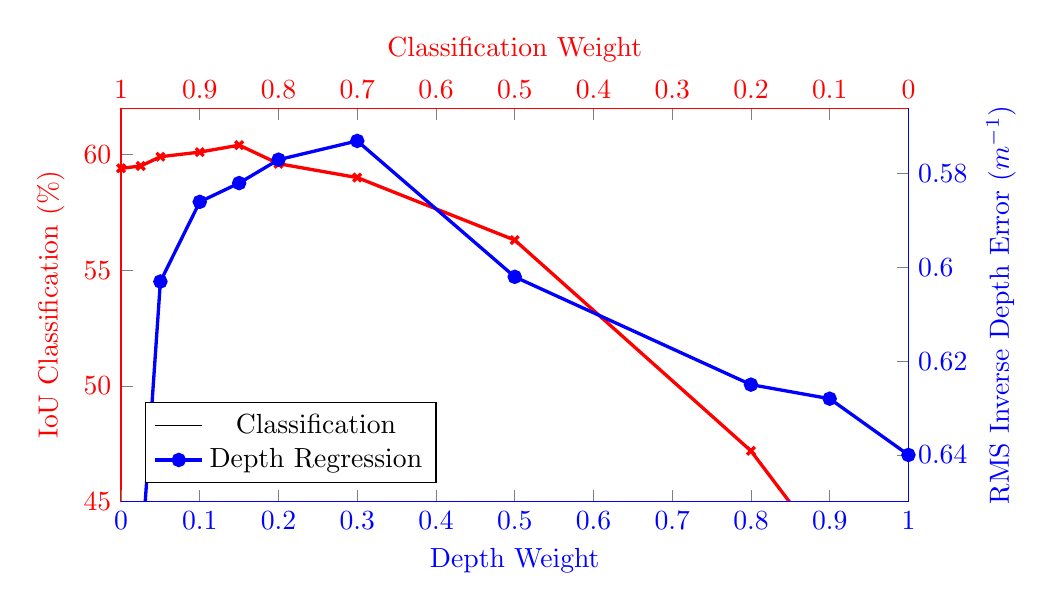
\begin{tikzpicture}
\pgfplotsset{
    compat=1.3,
    scale only axis,
    height=5cm,
    width=10cm, % \textwidth minus width of longest label text minus label offset
    legend style={at={(0.03,0.15)},anchor=west},
}

\pgfplotsset{
  axis line style={red},
  every axis label/.append style ={red},
  every tick label/.append style={red}  
}

\begin{axis}[
  axis y line*=left,
  axis x line*=top,
  ymin=45, ymax=62,
  x dir=reverse,
  xlabel=Classification Weight,
  ylabel=IoU Classification ($\%$),
  xmin=0, xmax=1,
]
\addplot[mark=x,red,very thick]
  coordinates{
    (1.0,59.4)
    (0.975,59.5)
    (0.95,59.9)
    (0.9,60.1)
    (0.85,60.4)
    (0.8,59.6)
    (0.7,59.0)
    (0.5,56.3)
    (0.2,47.2)
    (0.1,42.7)
}; \label{plot_one2}
\addlegendentry{Classification}
\end{axis}

\pgfplotsset{
  axis line style={blue},
  every axis label/.append style ={blue},
  every tick label/.append style={blue}  
}

\begin{axis}[
  axis y line*=right,
  axis x line*=bottom,
  xlabel=Depth Weight,
  xmin=0, xmax=1,
  ymin=0.566, ymax=0.65,
  ylabel=RMS Inverse Depth Error ($m^{-1}$),
  y dir=reverse,
]
\addlegendimage{/pgfplots/refstyle=plot_one2}\addlegendentry{Classification}
\addplot[mark=*,blue,very thick]
  coordinates{
    (0.025,0.664)
    (0.05,0.603)
    (0.1,0.586)
    (0.15,0.582)
    (0.2,0.577)
    (0.3,0.573)
    (0.5,0.602)
    (0.8,0.625)
    (0.9,0.628)
    (1.0,0.640)
}; \label{plot_two2}
\addlegendentry{Depth Regression}
\end{axis}
\end{tikzpicture}}
\end{subfigure}
\qquad\qquad
\begin{subfigure}[c]{0.2\linewidth}
\resizebox{\linewidth}{!}{
\begin{tabular}{cc|cc}
    \toprule
\multicolumn{2}{c|}{Task Weights} & Class & Depth \\
Class & Depth & IoU {[}$\%${]} & Err. {[}$px${]}\\
    \midrule
1.0 & 0.0 & 59.4 & - \\ %
0.975&0.025& 59.5 & 0.664 \\ % 
0.95& 0.05& 59.9 & 0.603 \\ %
0.9 & 0.1 & 60.1 & 0.586 \\ % 
0.85& 0.15& 60.4 & 0.582 \\ % 
0.8 & 0.2 & 59.6  & 0.577 \\ %
0.7 & 0.3 & 59.0 & 0.573 \\ %
0.5 & 0.5 & 56.3 & 0.602 \\ % 
0.2 & 0.8 & 47.2 & 0.625 \\ % 
0.1 & 0.9 & 42.7 & 0.628 \\ %
0.0 & 1.0 & - & 0.640 \\ %
    \midrule
\multicolumn{2}{c|}{\textbf{Learned weights}} & \multirow{3}{*}{\textbf{62.7}} & \multirow{3}{*}{\textbf{0.533}} \\
\multicolumn{2}{c|}{\textbf{with task uncertainty}} && \\
\multicolumn{2}{c|}{\textbf{(this work, \sct{mt_loss})}} && \\
    \bottomrule
\end{tabular}}
\end{subfigure}
\vspace{2pt}

(a) Comparing loss weightings when learning \textbf{semantic classification and depth regression}
%%%%%%%%%%%%%%%%%%%%%%%%%%%%%%%%%%%%%%%%%%%%%%%%%%%%%%%%%%%%%
%\noindent\rule{14cm}{0.4pt}

\begin{subfigure}[c]{0.4\linewidth}
\resizebox{\linewidth}{!}{
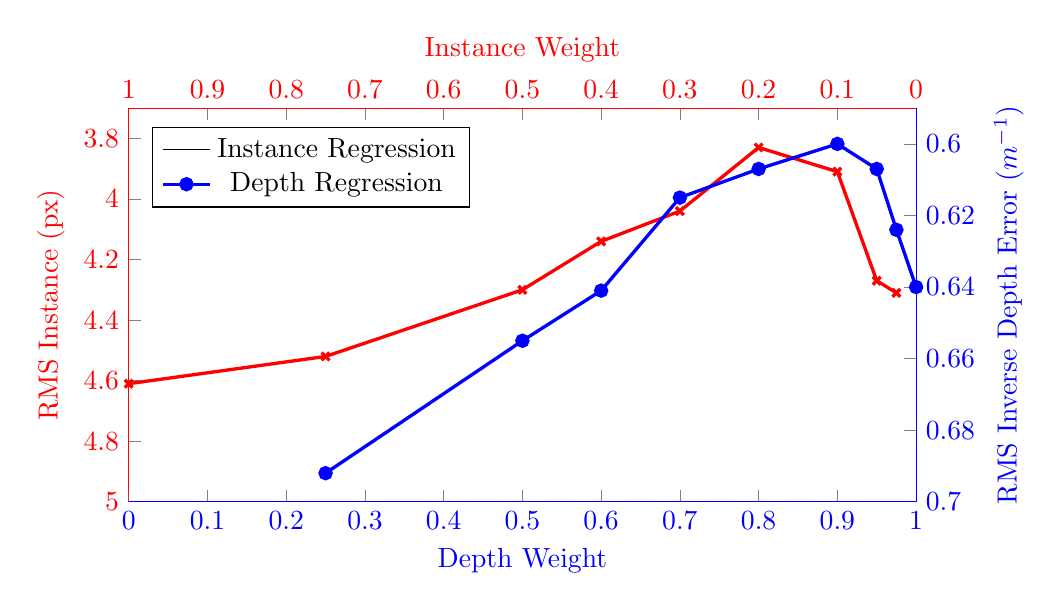
\begin{tikzpicture}
\pgfplotsset{
    compat=1.3,
    scale only axis,
    height=5cm,
    width=10cm, % \textwidth minus width of longest label text minus label offset
    legend style={at={(0.03,0.85)},anchor=west},
}

\pgfplotsset{
  axis line style={red},
  every axis label/.append style ={red},
  every tick label/.append style={red}  
}

\begin{axis}[
  axis y line*=left,
  axis x line*=top,
  ymin=3.7, ymax=5.0,
  x dir=reverse,
  xlabel=Instance Weight,
  ylabel=RMS Instance (px),
  xmin=0, xmax=1,
  y dir=reverse,
]
\addplot[mark=x,red,very thick]
  coordinates{
    (1.0,4.61)
    (0.75,4.52)
    (0.5,4.30)
    (0.4,4.14)
    (0.3,4.04)
    (0.2,3.83)
    (0.1,3.91)
    (0.05,4.27)
    (0.025,4.31)
}; \label{plot_one}
\addlegendentry{Instance Regression}
\end{axis}

\pgfplotsset{
  axis line style={blue},
  every axis label/.append style ={blue},
  every tick label/.append style={blue}  
}

\begin{axis}[
  axis y line*=right,
  axis x line*=bottom,
  xlabel=Depth Weight,
  xmin=0, xmax=1,
  ymin=0.59, ymax=0.7,
  ylabel=RMS Inverse Depth Error ($m^{-1}$),
  y dir=reverse,
]
\addlegendimage{/pgfplots/refstyle=plot_one}\addlegendentry{Instance Regression}
\addplot[mark=*,blue,very thick]
  coordinates{
    (0.25,0.692)
    (0.5,0.655)
    (0.6,0.641)
    (0.7,0.615)
    (0.8,0.607)
    (0.9,0.600)
    (0.95,0.607)
    (0.975,0.624)
    (1.0,0.640)
}; \label{plot_two}
\addlegendentry{Depth Regression}
\end{axis}
\end{tikzpicture}}
\end{subfigure}
\qquad\qquad
\begin{subfigure}[c]{0.2\linewidth}
\resizebox{\linewidth}{!}{
\begin{tabular}{cc|cc}
    \toprule
\multicolumn{2}{c|}{Task Weights} & Instance & Depth \\
Instance & Depth & Err. {[}$px${]} & Err. {[}$px${]}\\ 
    \midrule
1.0 & 0.0 & 4.61 &  \\
0.75 & 0.25 & 4.52 & 0.692 \\
0.5 & 0.5 & 4.30 & 0.655 \\
0.4 & 0.6 & 4.14 & 0.641 \\
0.3 & 0.7 & 4.04 & 0.615 \\
0.2 & 0.8 & 3.83 & 0.607 \\
0.1 & 0.9 & 3.91 & 0.600 \\
0.05 & 0.95 & 4.27 & 0.607 \\
0.025 & 0.975 & 4.31 & 0.624 \\
0.0 & 1.0 &  & 0.640 \\
    \midrule
\multicolumn{2}{c|}{\textbf{Learned weights}} & \multirow{3}{*}{\textbf{3.54}} & \multirow{3}{*}{\textbf{0.539}} \\
\multicolumn{2}{c|}{\textbf{with task uncertainty}} && \\
\multicolumn{2}{c|}{\textbf{(this work, \sct{mt_loss})}} && \\
    \bottomrule
\end{tabular}}
\end{subfigure}
%%%%%%%%%%%%%%%%%%%%%%%%%%%%%%%%%%%%%%%%%%%%%%%%%%%%%%%%%%%%%

(b) Comparing loss weightings when learning \textbf{instance regression and depth regression}
%\noindent\rule{14cm}{0.4pt}

   \caption[Effect of loss weighting in multi-task learning.]{\textbf{Learning multiple tasks improves the model's representation and individual task performance}. These figures and tables illustrate the advantages of multi-task learning for (a) semantic classification and depth regression and (b) instance and depth regression. Performance of the model in individual tasks is seen at both edges of the plot where $w=0$ and $w=1$. For some balance of weightings between each task, we observe improved performance for both tasks. All models were trained with a learning rate of $0.01$ with the respective weightings applied to the losses using the loss function in \eqn{basic_loss}. Results are shown using the Tiny CityScapes validation dataset using a down-sampled resolution of $128\times256$.}
\label{fig:scale_factor}
\end{figure*}
\end{landscape}
\clearpage% Flush page
}


\subsection{Multi Task Learning with Homoscedastic Uncertainty}
\label{sec:multitask}

Multi-task learning concerns the problem of optimising a model with respect to multiple objectives. It is prevalent in many deep learning problems. The naive approach to combining multi-objective losses would be to simply perform a weighted linear sum of the losses for each individual task:
\begin{equation}
\label{eqn:basic_loss}
L_{total}= \sum_i w_i L_{i}.
\end{equation}
This is the dominant approach used by prior work \citep{teichmann2016multinet,sermanet2013overfeat,liao2016understand,uhrig2016pixel}, for example for dense prediction tasks \citep{kokkinos2016ubernet}, for scene understanding tasks \citep{eigen2015predicting} and for rotation (in quaternions) and translation (in meters) for camera pose \citep{kendall2015posenet}. However, there are a number of issues with this method. Namely, model performance is extremely sensitive to weight selection, $w_i$, as illustrated in \fig{scale_factor}. These weight hyper-parameters are expensive to tune, often taking many days for each trial. Therefore, it is desirable to find a more convenient approach which is able to learn the optimal weights.

More concretely, let us consider a network which learns to predict pixel-wise depth and semantic class from an input image. In \fig{scale_factor} the two boundaries of each plot show models trained on individual tasks, with the curves showing performance for varying weights $w_i$ for each task. We observe that at some optimal weighting, the joint network performs better than separate networks trained on each task individually (performance of the model on individual tasks is seen at both edges of the plot: $w=0$ and $w=1$). At near-by values to the optimal weight the network performs worse on one of the tasks. However, searching for these optimal weightings is expensive and increasingly difficult with large models with numerous tasks. \fig{scale_factor} also shows a similar result for two regression tasks; instance segmentation and depth regression. We next show how to learn optimal task weightings using ideas from probabilistic modelling.

\subsection{Homoscedastic uncertainty as task-dependent uncertainty}
\label{sec:uncertainty}

In Bayesian modelling, there are two main types of uncertainty one can model \citep{kendall2017uncertainties}.
\begin{itemize}
\item \textit{Epistemic uncertainty} is uncertainty in the model, which captures what our model does not know due to lack of training data. It can be explained away with increased training data.
\item \textit{Aleatoric uncertainty} captures our uncertainty with respect to information which our data cannot explain. Aleatoric uncertainty can be explained away with the ability to observe all explanatory variables with increasing precision.
\end{itemize}
Aleatoric uncertainty can again be divided into two sub-categories.
\begin{itemize}
\item \textit{Data-dependent} or \textit{Heteroscedastic} uncertainty is aleatoric uncertainty which depends on the input data and is predicted as a model output.
\item \textit{Task-dependent} or \textit{Homoscedastic} uncertainty is  aleatoric uncertainty which is not dependent on the input data. It is not a model output, rather it is a quantity which stays constant for all input data and varies between different tasks. It can therefore be described as task-dependent uncertainty.
\end{itemize}
In a multi-task setting, we show that the task uncertainty captures the relative confidence between tasks, reflecting the uncertainty inherent to the regression or classification task. It will also depend on the task's representation or unit of measure.  We propose that we can use homoscedastic uncertainty as a basis for weighting losses in a multi-task learning problem.

\subsection{Multi-task likelihoods}
\label{sec:mt_loss}

In this section we derive a multi-task loss function based on maximising the Gaussian likelihood with homoscedastic uncertainty.
This extends the derivation in \cref{sect:hetero} to multi-task likelihoods.
Let $\f^\W(\x)$ be the output of a neural network with weights $\W$ on input $\x$. We define the following probabilistic model. 
For regression tasks we define our likelihood as a Gaussian with mean given by the model output:
\begin{equation}
p(\y | \f^\W(\x)) = \N(\f^\W(\x), \sigma^2)
\end{equation}
with an observation noise scalar $\sigma$. 
For classification we often squash the model output through a softmax function, and sample from the resulting probability vector:
% \newcommand{\softmax}{\text{softmax}}
\begin{equation}
p(\y | \f^\W(\x)) = \softmax(\f^\W(\x)).
\end{equation}

In the case of multiple model outputs, we often define the likelihood to factorise over the outputs, given some sufficient statistics. We define $\f^\W(\x)$ as our sufficient statistics, and obtain the following multi-task likelihood:
\begin{equation}
p(\y_1, ..., \y_K | \f^\W(\x)) = p(\y_1 | \f^\W(\x)) ... p(\y_K | \f^\W(\x))
\end{equation}
with model outputs $\y_1, ..., \y_K$ (such as semantic segmentation, depth regression, etc).

In \textit{maximum likelihood} inference, we maximise the log likelihood of the model.
In regression, for example, the log likelihood can be written as
\begin{equation}
\log p(\y | \f^{\W}(\x)) \propto 
-\frac{1}{2 \sigma^2}||\y - \f^{\W}(\x)||^2 - \log \sigma
\end{equation}
for a Gaussian likelihood (or similarly for a Laplace likelihood)
% \begin{align*}
% \log p(\y | \f^{\W}(\x)) \propto 
% -\frac{1}{\sigma^2}||\y - \f^{\W}(\x)|| - \log \sigma^2 
% \end{align*}
% for a Laplace likelihood,
with $\sigma$ the model's observation noise parameter -- capturing how much noise we have in the outputs. We then maximise the log likelihood with respect to the model parameters $\W$ and observation noise parameter $\sigma$.

Let us now assume that our model output is composed of two vectors $\y_1$ and $\y_2$, each following a Gaussian distribution:
\begin{equation}
\begin{split}
p(\y_1, \y_2 | \f^\W(\x)) &= 
p(\y_1 | \f^\W(\x)) \cdot p(\y_2 | \f^\W(\x)) \\
&= 
\N(\y_1; \f^\W(\x), \sigma_1^2) \cdot
\N(\y_2; \f^\W(\x), \sigma_2^2).
\end{split}
\end{equation}

This leads to the \textit{minimisation} objective, $\cL(\W, \sigma_1, \sigma_2)$, (our loss) for our multi-output model:
\begin{equation}
\begin{split}
 &= 
- \log p(\y_1, \y_2 | \f^\W(\x)) \\
&\propto
\frac{1}{2 \sigma_1^2} ||\y_1 - \f^{\W}(\x)||^2
+ \frac{1}{2 \sigma_2^2} ||\y_2 - \f^{\W}(\x)||^2 
+ \log \sigma_1 \sigma_2 \\
&= \frac{1}{2 \sigma_1^2} \cL_1(\W) 
+ \frac{1}{2 \sigma_2^2} \cL_2(\W)
+ \log \sigma_1 \sigma_2
\end{split}
\end{equation}
Where we write $\cL_1(\W) = ||\y_1 - \f^{\W}(\x)||^2$ for the loss of the first output variable, and similarly for $\cL_2(\W)$.

% Rewriting this objective 

We interpret minimising this last objective with respect to $\sigma_1$ and $\sigma_2$ as learning the relative weight of the losses $\cL_1(\W)$ and $\cL_2(\W)$ adaptively, based on the data. As $\sigma_1$ -- the noise parameter for the variable $\y_1$ -- increases, we have that the weight of $\cL_1(\W)$ decreases. On the other hand, as the noise decreases, we have that the weight of the respective objective increases. The noise is discouraged from increasing too much (effectively ignoring the data) by the last term in the objective, which acts as a regulariser for the noise terms.

This construction can be trivially extended to multiple regression outputs. However, the extension to classification likelihoods is more interesting. We adapt the classification likelihood to squash a \textit{scaled} version of the model output through a softmax function:
\begin{equation}
p(\y | \f^\W(\x), \sigma) = \softmax \bigg( \frac{1}{\sigma^2} \f^\W(\x) \bigg)
\end{equation}
with a positive scalar $\sigma$. 
This can be interpreted as a Boltzmann distribution (also called Gibbs distribution) where the input is scaled by $\sigma^2$ (often referred to as \textit{temperature}). This scalar is either fixed or can be learnt, where the parameter's magnitude determines how `uniform' (flat) the discrete distribution is. This relates to its uncertainty, as measured in entropy.
The log likelihood for this output can then be written as 
\begin{equation}
\begin{split}
\log p(\y = c | \f^\W(\x), \sigma) &= \frac{1}{\sigma^2} f^\W_c(\x) \\
&- \log \sum_{c'} \exp \bigg( \frac{1}{\sigma^2} f^\W_{c'}(\x) \bigg)
\end{split}
\end{equation}
with $f^\W_c(\x)$ the $c$'th element of the vector $\f^\W(\x)$. 
% We can rewrite this log likelihood in terms of $\cL(\W) = - \log \softmax (\f^\W(\x))$, the cross entropy loss:
% \begin{align*}
% \log p(\y = c | \f^\W(\x), \sigma) 
% &= 
% - \frac{1}{\sigma^2} \cL(\W)
% + \frac{1}{\sigma^2} \log \sum_{c'} \exp \bigg( f^\W_{c'}(\x) \bigg)
% - \log \sum_{c'} \exp \bigg( \frac{1}{\sigma^2} f^\W_{c'}(\x) \bigg)
% \\
% % &= 
% % \frac{1}{\sigma^2} \cL(\W)
% % + \log \bigg( \sum_{c'} \exp \bigg( f^\W_{c'}(\x) \bigg) \bigg)^{\frac{1}{\sigma^2} }
% % - \log \sum_{c'} \exp \bigg( \frac{1}{\sigma^2} f^\W_{c'}(\x) \bigg)
% % \\
% &= 
% -\frac{1}{\sigma^2} \cL(\W)
% - \log \frac{
% \sum_{c'} \exp \bigg( \frac{1}{\sigma^2} f^\W_{c'}(\x) \bigg)
% }{
% \bigg( \sum_{c'} \exp \bigg( f^\W_{c'}(\x) \bigg) \bigg)^{\frac{1}{\sigma^2} }
% }.
% \end{align*}

Next, assume that a model's multiple outputs are composed of a continuous output $\y_1$ and a discrete output $\y_2$, modelled with a Gaussian likelihood and a softmax likelihood, respectively. Like before, the joint loss, $\cL(\W, \sigma_1, \sigma_2)$, is given as:
\begin{equation}
\begin{aligned}
 &= 
-\log p(\y_1, \y_2=c | \f^\W(\x)) \\
&= 
-\log \N(\y_1; \f^\W(\x), \sigma_1^2) \cdot
\softmax(\y_2=c; \f^\W(\x), \sigma_2) \\
&=
\frac{1}{2 \sigma_1^2} ||\y_1 - \f^{\W}(\x)||^2
+ \log \sigma_1
- \log p(\y_2 = c | \f^\W(\x), \sigma_2)
 \\
&= \frac{1}{2 \sigma_1^2} \cL_1(\W) 
+ \frac{1}{\sigma_2^2} \cL_2(\W)
+ \log \sigma_1 \\
&\quad\quad\quad\quad + \log \frac{
\sum_{c'} \exp \bigg( \frac{1}{\sigma_2^2} f^\W_{c'}(\x) \bigg)
}{
\bigg( \sum_{c'} \exp \bigg( f^\W_{c'}(\x) \bigg) \bigg)^{\frac{1}{\sigma_2^2} }
}
\\
&\approx \frac{1}{2 \sigma_1^2} \cL_1(\W) 
+ \frac{1}{\sigma_2^2} \cL_2(\W)
+ \log \sigma_1
+ \log \sigma_2,
\end{aligned}
\end{equation}
where again we write $\cL_1(\W) = ||\y_1 - \f^{\W}(\x)||^2$ for the Euclidean loss of $\y_1$, write $\cL_2(\W) = -\log \softmax (\y_2, \f^\W(\x))$ for the cross entropy loss of $\y_2$ (with $\f^{\W}(\x)$ not scaled), and optimise with respect to $\W$ as well as $\sigma_1$, $\sigma_2$.
In the last transition we introduced the explicit simplifying assumption $\frac{1}{\sigma_2} \sum_{c'} \exp \bigg( \frac{1}{\sigma_2^2} f^\W_{c'}(\x) \bigg) \approx \bigg( \sum_{c'} \exp \bigg( f^\W_{c'}(\x) \bigg) \bigg)^{\frac{1}{\sigma_2^2} }$ which becomes an equality when $\sigma_2 \rightarrow 1$. This has the advantage of simplifying the optimisation objective, as well as empirically improving results.

This last objective can be seen as learning the relative weights of the losses for each output. Large scale values $\sigma_2$ will decrease the contribution of $\cL_2(\W)$, whereas small scale $\sigma_2$ will increase its contribution. The scale is regulated by the last term in the equation. The objective is penalised when setting $\sigma_2$ too large. % (with the last term contributing a constant value $\log C$ -- with $C$ classes -- to the loss). 

% However, we observe that scaling the logits in the SoftMax cross entropy loss does not add any additional modelling capacity. This is because the neural network is free to output logits with any arbitrary scale of its choosing from the final affine regression layer. We do not observe any improvement by using this loss, as the network compensates for the homoscedastic uncertainty, such that the net effect of this pre-softmax scaling is zero. This suggests why multi-task learning with a sum of classification losses has been successful in the past \citep{uhrig2016pixel,kokkinos2016ubernet} -- the SoftMax function inherently captures homoscedastic uncertainty.

% What we observe when classification and regression losses are combined, is that the classification loss is under-weighted compared to the best performing weighting found through grid search. The data terms, $x$, in the regularisation term restrict the weighting compared to regression functions. Ideally, we would like to give the model capacity to freely increase the SoftMax cross entropy loss if required. For this reason, we reconsider the SoftMax cross entropy loss as a distance metric. Cross entropy is a divergence, and not strictly a distance because it is not symmetric. However, we approximate it as a distance which allows us to use the regression objective and remove the input, $x$, from the regularisation term. 
%The multi-task objective with homoscedastic task uncertainty now becomes:
%\begin{equation}
%\cL(\W, \sigma_1, \sigma_2, ..., \sigma_i) = \sum_i \frac{1}{2 \sigma_i^2} \cL_i(\W) + \log \sigma_i
%\label{eqn:loss}
%\end{equation}
%over all tasks indexed by $i$. Again, we write $\cL_i(\W) = ||\y_i - \f^{\W}(\x)||^2$ for regression losses $\y_i$, and $\cL_i(\W) = -\log \softmax (\y_i, \f^\W(\x))$ for classification losses. 

This construction can be trivially extended to arbitrary combinations of discrete and continuous loss functions, allowing us to learn the relative weights of each loss in a principled and well-founded way. This loss is smoothly differentiable, and is well formed such that the task weights will not converge to zero. In contrast, directly learning the weights using a simple linear sum of losses \eqn{basic_loss} would result in weights which quickly converge to zero. In the following sections we introduce our experimental model and present empirical results.

In practice, we train the network to predict the log variance, $s := \log \sigma^2$.
This is because it is more stable than regressing the variance, $\sigma^2$, as the loss avoids any division by zero. The exponential mapping also allows us to regress unconstrained scalar
values, where $\exp(-s)$ is resolved to the positive domain giving valid values for variance.

%Our final learning objective is,
%\begin{equation}
%\cL = 2 \exp(-s_C)  \cL_C 
%+ \exp(-s_I)  \cL_I
%+ \exp(-s_D)  \cL_D
%+ s_C + s_I + s_D,
%\end{equation}

%%%%%%%%%%%%%%%%%%%%%%%%%%%%%%%%%%%%%%%%%%%%%%%%%%%%%%%%%%%%%%%%%%%%%%%%%%%%%%%%%%%%%%%%%%%%%%

\subsection{Scene Understanding Tasks}
\label{sec:arch}

To understand semantics and geometry we first propose an architecture which can learn regression and classification outputs, at a pixel level. Our architecture is a deep convolutional encoder decoder network \citep{badrinarayanan2017segnet}. Our model consists of a number of convolutional encoders which produce a shared representation, followed by a number of task-specific convolutional decoders. A high level summary is shown in \fig{teaser}. The purpose of the encoder is to learn a deep mapping to produce rich, contextual features, using domain knowledge from a number of related tasks. The purpose of the decoder is to learn a mapping from the shared features to an output. This section describes how we learn each of the scene understanding tasks.

\textbf{Semantic Segmentation.}
We use the cross-entropy loss to learn pixel-wise class probabilities, averaging the loss over the pixels with semantic labels in each mini-batch.
%$\cL_{class}(\W) = \frac{1}{|N_C|} \sum_{N_C} -\log \softmax (\y_i, \f^\W(\x))$. We average the loss over the pixels with semantic labels in each mini-batch, $N_C$. 

\textbf{Instance Segmentation.}
An intuitive method for defining which instance a pixel belongs to is an association to the instance's centroid.
% In a practical setting, it is extremely unlikely two instances share the same centroid. 
We use a regression approach for instance segmentation \citep{liang2015proposal}. This approach is inspired by \citep{leibe2008robust} which identifies instances using Hough votes from object parts. In this work we extend this idea by using votes from individual pixels using deep learning. We learn an instance vector, $\hat{x}_n$, for each pixel coordinate, $c_n$, which points to the centroid of the pixel's instance, $i_n$, such that $i_n=\hat{x}_n+c_n$. We train this regression with an $L_1$ loss using ground truth labels $x_n$, averaged over all labelled pixels, $N_I$, in a mini-batch: $\cL_{Instance} = \frac{1}{|N_I|} \sum_{N_I} \norm{x_n - \hat{x}_n}_1$.

\fig{instance} details the representation we use for instance segmentation. \fig{instance}(a) shows the input image and a mask of the pixels which are of an instance class (at test time inferred from the predicted semantic segmentation). \fig{instance}(b) and \fig{instance}(c) show the ground truth and predicted instance vectors for both $x$ and $y$ coordinates. We then cluster these votes using OPTICS \citep{ankerst1999optics}, resulting in the predicted instance segmentation output in \fig{instance}(d).

\begin{figure}[t]
\begin{center}
\begin{subfigure}[t]{0.48\linewidth}
  \includegraphics[width=\linewidth]{example_instance/bielefeld_000000_001011_leftImg8bit.png}
  \caption{Input Image}
\end{subfigure}
\begin{subfigure}[t]{0.48\linewidth}
  \includegraphics[width=\linewidth]{example_instance/bielefeld_000000_001011_semantic_segmentation_rgb.png}
  \caption{Semantic Segmentation}
\end{subfigure}
\begin{subfigure}[t]{0.48\linewidth}
  \includegraphics[width=\linewidth]{example_instance/bielefeld_000000_001011_instance_prediction.png}
  \caption{Instance vector regression}
\end{subfigure}
\begin{subfigure}[t]{0.48\linewidth}
  \includegraphics[width=\linewidth]{example_instance/bielefeld_000000_001011_instance_segmentation.png}
  \caption{Instance Segmentation}
\end{subfigure}
\end{center}
   \caption[Instance centroid regression method.]{\textbf{Instance centroid regression method.} For each pixel, we regress a vector pointing to the instance's centroid. The loss is only computed over pixels which are from instances. We visualise (c) by representing colour as the orientation of the instance vector, and intensity as the magnitude of the vector.}
\label{fig:instance}
\end{figure}

One of the most difficult cases for instance segmentation algorithms to handle is when the instance mask is split due to occlusion. \fig{instancemask} shows that our method can handle these situations, by allowing pixels to vote for their instance centroid with geometry. Methods which rely on watershed approaches \citep{bai2016deep}, or instance edge identification approaches fail in these scenarios.

To obtain segmentations for each instance, we now need to estimate the instance centres, $\hat{i}_n$. We propose to consider the estimated instance vectors, $\hat{x}_n$, as votes in a Hough parameter space and use a clustering algorithm to identify these instance centres. OPTICS \citep{ankerst1999optics}, is an efficient density based clustering algorithm. It is able to identify an unknown number of multi-scale clusters with varying density from a given set of samples. We chose OPTICS for two reasons. Crucially, it does not assume knowledge of the number of clusters like algorithms such as k-means \citep{macqueen1967some}. Secondly, it does not assume a canonical instance size or density like discretised binning approaches \citep{comaniciu2002mean}. Using OPTICS, we cluster the points $c_n+\hat{x}_n$ into a number of estimated instances, $\hat{i}$. We can then assign each pixel, $p_n$ to the instance closest to its estimated instance vector, $c_n+\hat{x}_n$.

\textbf{Depth Regression.}
We train with supervised labels using pixel-wise metric inverse depth using a $L_1$ loss function: $\cL_{Depth} = \frac{1}{|N_D|} \sum_{N_D} \norm{d_n-\hat{d_n}}_1$. Our architecture estimates inverse depth, $\hat{d}_n$, because it can represent points at infinite distance (such as sky). We can obtain inverse depth labels, $d_n$, from a RGBD sensor or stereo imagery. Pixels which do not have an inverse depth label are ignored in the loss.


\begin{figure}[t]
\begin{center}
\begin{subfigure}[t]{0.49\linewidth}
  \includegraphics[width=\linewidth,trim={350px 120px 0 100px},clip]{example_instance/segnet_19_output_0.jpg}
  \caption{Input Image}
\end{subfigure}
\begin{subfigure}[t]{0.49\linewidth}
  \includegraphics[width=\linewidth,trim={350px 120px 0 100px},clip]{example_instance/segnet_19_output_3.png}
  \caption{Instance Segmentation}
\end{subfigure}
\end{center}
   \caption[Instance segmentation with occlusion.]{This example shows two cars which are occluded by trees and lampposts, making the instance segmentation challenging. Our instance segmentation method can handle occlusions effectively. We can correctly handle segmentation masks which are split by occlusion, yet part of the same instance, by incorporating semantics and geometry.}
\label{fig:instancemask}
\end{figure}


\subsection{Model Architecture}
We base our model on the recently introduced DeepLabV3 \citep{chen2017rethinking} segmentation architecture.
%We use \citep{wideresnet} as our base feature encoder (pretrained by \citep{bulo2017place}), with dilated convolutions, resulting in a feature map which is downsampled by a factor of 8 compared with the original input image. 
We use ResNet101 \citep{he2016deep} as our base feature encoder, with dilated convolutions, resulting in a feature map which is downsampled by a factor of 8 compared with the original input image. 
We then append dilated (atrous) convolutional ASPP module \citep{chen2017rethinking}. This module is designed to improve the contextual reasoning of the network. We use an ASPP module comprised of four parallel convolutional layers, with 256 output channels and dilation rates (1, 12, 24, 36), with kernel sizes ($1^2$, $3^2$, $3^2$, $3^2$). Additionally, we also apply global average pooling to the encoded features, and convolve them to 256 dimensions with a $1 \times 1$ kernel. We apply batch normalisation to each of these layers and concatenate the resulting 1280 features together. This produces the shared representation between each task.

We then split the network, to decode this representation to a given task output. For each task, we construct a decoder consisting of two layers. First, we apply a $1 \times 1$ convolution, outputting 256 features, followed by batch normalisation and a non-linear activation. Finally, we convolve this output to the required dimensions for a given task. For classification, this will be equal to the number of semantic classes, otherwise the output will be 1 or 2 channels for depth or instance segmentation respectively. Finally, we apply bilinear upsampling
to scale the output to the same resolution as the input.

The majority of the model's parameters and depth is in the feature encoding, with very little flexibility in each task decoder. This illustrates the attraction of multi-task learning; most of the compute can be shared between each task to learn a better shared representation.

\subsubsection{Optimisation.}
For all experiments, we use an initial learning rate of $2.5\times10^{-3}$ and polynomial learning rate decay $(1-\frac{iter}{max~iter})^{0.9}$. We train using stochastic gradient descent, with Nesterov updates and momentum $0.9$ and weight decay $10^{-4}$. We conduct all experiments in this paper using PyTorch.

For the experiments on the Tiny CityScapes validation dataset (using a down-sampled resolution of $128\times256$) we train over $50,000$ iterations, using $256 \times 256$ crops with batch size of 8 on a single NVIDIA 1080Ti GPU. We apply random horizontal flipping to the data.

For the full-scale CityScapes benchmark experiment, we train over $100,000$ iterations with a batch size of 16. We apply random horizontal flipping (with probability 0.5) and random scaling (selected from 0.7 - 2.0) to the data during training, before making a $512 \times 512$ crop. The training data is sampled uniformly, and is randomly shuffled for each epoch. Training takes five days on a single computer with four NVIDIA 1080Ti GPUs.

\subsection{Experiments}
\label{sec:model_analysis_mt}

We demonstrate the efficacy of our method on CityScapes \citep{Cordts2016Cityscapes}, a large dataset for road scene understanding. It comprises of stereo imagery, from automotive grade stereo cameras with a $22cm$ baseline, labelled with instance and semantic segmentations from 20 classes. Depth images are also provided, labelled using SGM \citep{Hirschmuller2008}, which we treat as pseudo ground truth. Additionally, we assign zero inverse depth to pixels labelled as sky. The dataset was collected from a number of cities in fine weather and consists of 2,975 training and 500 validation images at $2048\times1024$ resolution. 1,525 images are withheld for testing on an online evaluation server.

\afterpage{%
    \clearpage% Flush earlier floats (otherwise order might not be correct)
    \begin{landscape}% Landscape page
    \centering
\begin{table*}[t]
\centering
%\resizebox{\textwidth}{!}{
\begin{tabular}{l|ccc|c|c|c}
    \toprule
& \multicolumn{3}{c|}{Task Weights} & Segmentation & Instance & Inverse Depth \\
Loss & Seg. & Inst. & Depth & IoU {[}$\%${]} & Mean Error {[}$px${]} & Mean Error {[}$px${]}\\ 
    \midrule
Segmentation only & 1 & 0 & 0 & 59.4\% &-&-\\
Instance only & 0 & 1 & 0 &-& 4.61 &-\\
Depth only & 0 & 0 & 1 &-&-& 0.640 \\ 
    \midrule
Unweighted sum of losses & 0.333 & 0.333 & 0.333 & 50.1\% & 3.79 & 0.592 \\
    \midrule
Approx. optimal weights & 0.89 & 0.01 & 0.1 & 62.8\% & 3.61 & 0.549 \\
    \midrule
2 task uncertainty weighting & \checkmark & \checkmark & & 61.0\% & \textbf{3.42} & - \\%done
2 task uncertainty weighting & \checkmark & & \checkmark & 62.7\% & - & 0.533 \\%done
2 task uncertainty weighting & & \checkmark & \checkmark & - & 3.54 & 0.539 \\%underway
    \midrule
3 task uncertainty weighting & \checkmark & \checkmark & \checkmark & \textbf{63.4\%} & 3.50 & \textbf{0.522} \\ %underway
    \bottomrule
\end{tabular}
\caption[Quantitative results.]{Quantitative improvement when learning semantic segmentation, instance segmentation and depth with our multi-task loss. Experiments were conducted on the Tiny CityScapes dataset (sub-sampled to a resolution of $128\times 256$). Results are shown from the validation set. We observe an improvement in performance when training with our multi-task loss, over both single-task models and weighted losses. Additionally, we observe an improvement when training on all three tasks ($3\times \checkmark$) using our multi-task loss, compared with all pairs of tasks alone (denoted by $2\times \checkmark$). This shows that our loss function can automatically learn a better performing weighting between the tasks than the baselines.}
\label{tbl:multitasks}
\end{table*}
\end{landscape}
\clearpage% Flush page
}

In \tbl{multitasks} we compare individual models to multi-task learning models using a na{\"i}ve weighted loss or the task uncertainty weighting we propose in this paper. To reduce the computational burden, we train each model at a reduced resolution of $128\times256$ pixels, over $50,000$ iterations. When we downsample the data by a factor of four, we also need to scale the disparity labels accordingly. \tbl{multitasks} clearly illustrates the benefit of multi-task learning, which obtains significantly better performing results than individual task models. For example, using our method we improve classification results from $59.4\%$ to $63.4\%$.

We also compare to a number of na{\"i}ve multi-task losses. We compare weighting each task equally and using approximately optimal weights. Using a uniform weighting results in poor performance, in some cases not even improving on the results from the single task model. Obtaining approximately optimal weights is difficult with increasing number of tasks as it requires an expensive grid search over parameters. However, even these weights perform worse compared with our proposed method. \fig{scale_factor} shows that using task uncertainty weights can even perform better compared to optimal weights found through fine-grained grid search. We believe that this is due to two reasons. First, grid search is restricted in accuracy by the resolution of the search. Second, optimising the task weights using a homoscedastic noise term allows for the weights to be dynamic during training. In general, we observe that the uncertainty term decreases during training which improves the optimisation process.


\begin{figure*}[t]
\resizebox{\linewidth}{!}{
\begin{subfigure}[t]{0.24\linewidth}
\begin{center}
		\includegraphics[width=\linewidth,trim={0px 60px 0 0px},clip]{qualitative/bielefeld_000000_026550_leftImg8bit.jpg}
		\includegraphics[width=\linewidth,trim={0px 60px 0 0px},clip]{qualitative/bonn_000045_000019_leftImg8bit.jpg}
		\includegraphics[width=\linewidth,trim={0px 60px 0 0px},clip]{qualitative/munich_000021_000019_leftImg8bit.jpg}
		\includegraphics[width=\linewidth,trim={0px 60px 0 0px},clip]{qualitative/munich_000042_000019_leftImg8bit.jpg}
  \caption{Input image}
\end{center}
\end{subfigure}
\begin{subfigure}[t]{0.24\linewidth}
\begin{center}
		\includegraphics[width=\linewidth,trim={0px 60px 0 0px},clip]{qualitative/bielefeld_000000_026550_semantic_segmentation_rgb.jpg}
		\includegraphics[width=\linewidth,trim={0px 60px 0 0px},clip]{qualitative/bonn_000045_000019_semantic_segmentation_rgb.jpg}
		\includegraphics[width=\linewidth,trim={0px 60px 0 0px},clip]{qualitative/munich_000021_000019_semantic_segmentation_rgb.jpg}
		\includegraphics[width=\linewidth,trim={0px 60px 0 0px},clip]{qualitative/munich_000042_000019_semantic_segmentation_rgb.jpg}
  \caption{Segmentation output}
\end{center}
\end{subfigure}
\begin{subfigure}[t]{0.24\linewidth}
\begin{center}
		\includegraphics[width=\linewidth,trim={0px 60px 0 0px},clip]{qualitative/bielefeld_000000_026550_instance_segmentation.jpg}
		\includegraphics[width=\linewidth,trim={0px 60px 0 0px},clip]{qualitative/bonn_000045_000019_instance_segmentation.jpg}
		\includegraphics[width=\linewidth,trim={0px 60px 0 0px},clip]{qualitative/munich_000021_000019_instance_segmentation.jpg}
		\includegraphics[width=\linewidth,trim={0px 60px 0 0px},clip]{qualitative/munich_000042_000019_instance_segmentation.jpg}
  \caption{Instance output}
\end{center}
\end{subfigure}
\begin{subfigure}[t]{0.24\linewidth}
\begin{center}
		\includegraphics[width=\linewidth,trim={0px 60px 0 0px},clip]{qualitative/bielefeld_000000_026550_depth_prediction.jpg}
		\includegraphics[width=\linewidth,trim={0px 60px 0 0px},clip]{qualitative/bonn_000045_000019_depth_prediction.jpg}
		\includegraphics[width=\linewidth,trim={0px 60px 0 0px},clip]{qualitative/munich_000021_000019_depth_prediction.jpg}
		\includegraphics[width=\linewidth,trim={0px 60px 0 0px},clip]{qualitative/munich_000042_000019_depth_prediction.jpg}
  \caption{Depth output}
\end{center}
\end{subfigure}}
	\caption[Qualitative results.]{\textbf{Qualitative results for multi-task learning of geometry and semantics for road scene understanding with a single network trained on all tasks}. We observe that multi-task learning improves the smoothness and accuracy for depth perception because it learns a representation that uses cues from other tasks, such as segmentation (and vice versa).}
	\label{fig:cityscapesqual}
\end{figure*}

We benchmark our model using the full-size CityScapes dataset. In \tbl{benchmarks} we compare to a number of other state of the art methods in all three tasks. Our method is the first model which completes all three tasks with a single model. We compare favourably with other approaches, outperforming many which use comparable training data and inference tools. \fig{cityscapesqual} shows some qualitative examples of our model.



\afterpage{%
    \clearpage% Flush earlier floats (otherwise order might not be correct)
    \begin{landscape}% Landscape page
    \centering
\begin{table*}[t]
	\centering
	\resizebox{\linewidth}{!}{
		\begin{tabular}{l|c|c|c|c|c|c|c|c|c|c}
        \toprule
			& \multicolumn{4}{c|}{Semantic Segmentation} & \multicolumn{4}{c|}{Instance Segmentation} & \multicolumn{2}{c}{Monocular Disparity Estimation} \\
			Method & IoU class & iIoU class & IoU cat & iIoU cat & AP & AP 50\% & AP 100m & AP 50m & Mean Error {[}$px${]} & RMS Error {[}$px${]} \\ \toprule % & Runtime [s]\\ \hline \hline
			\multicolumn{11}{c}{\textbf{Semantic segmentation, instance segmentation and depth regression methods (this work)}}\\ \midrule
			Multi-Task Learning & 78.5 & 57.4 & 89.9 & 77.7 & 21.6 & 39.0 & 35.0 & 37.0 & 2.92 & 5.88 \\ \midrule%& - \\
			\multicolumn{11}{c}{\textbf{Semantic segmentation and instance segmentation methods}}\\ \midrule
			Uhrig et al. \citep{uhrig2016pixel} & 64.3 & 41.6 & 85.9 & 73.9 & 8.9 & 21.1 & 15.3 & 16.7 &-&-\\ \midrule%& - \\ \hline
			\multicolumn{11}{c}{\textbf{Instance segmentation only methods}}\\ \midrule
			Mask R-CNN \citep{he2017maskrcnn} &-&-&-&-& 26.2 & 49.9 & 37.6 & 40.1 & -& -\\ %& 60.0 \\ \hline
            Deep Watershed \citep{bai2016deep} &-&-&-&-& 19.4 & 35.3 & 31.4 & 36.8 & -& -\\ %& 60.0 \\ \hline
            R-CNN + MCG \citep{Cordts2016Cityscapes} &-&-&-&-& 4.6 & 12.9 & 7.7 & 10.3 & -& -\\ \midrule %& 60.0 \\ \hline
			\multicolumn{11}{c}{\textbf{Semantic segmentation only methods}}\\ \midrule
			DeepLab V3 \citep{chen2017rethinking} & 81.3 & 60.9 & 91.6 & 81.7 &-&-&-&-&-&-\\%& 
			PSPNet \citep{zhao2017pspnet} & 81.2 & 59.6 & 91.2 & 79.2 &-&-&-&-&-&-\\%& 
			%LRR-4x \citep{ghiasi2016laplacian} & 71.8 & 47.9 & 88.4 & 73.9 &-&-&-&-&-&-\\%& 
			Adelaide \citep{lin2015efficient} & 71.6 & 51.7 & 87.3 & 74.1 &-&-&-&-&-&-\\%& 4.0\\
			%DeepLab \citep{chen2016deeplab} & 70.4 & 42.6 & 86.4 & 67.7 &-&-&-&-&-&-\\%& 4.0\\
			%Dilation \citep{YuKoltun2016} & 67.1 & 42.0 & 86.5 & 71.1 &-&-&-&-&-&-\\%& 4.0 \\
			%FCN 8s \citep{long2014fully} & 65.3 & 41.7 & 85.7 & 70.1 &-&-&-&-&-&-\\%& 0.5 \\
			%SegNet \citep{badrinarayanan2017segnet} & 57.0 & 32.0 & 79.1 & 61.9 &-&-&-&-&-&-\\%& 0.06 \\
            \bottomrule
		\end{tabular}}
	\caption[CityScapes Benchmark.]{\textbf{CityScapes Benchmark \citep{Cordts2016Cityscapes}.} We show results from the test dataset using the full resolution of $1024\times2048$ pixels. For the full leaderboard, please see \url{www.cityscapes-dataset.com/benchmarks}. The disparity (inverse depth) metrics were computed against the CityScapes depth maps, which are sparse and computed using SGM stereo \citep{hirschmuller2005accurate}. Note, these comparisons are not entirely fair, as many methods use ensembles of different training datasets. Our method is the first to address all three tasks with a single model.}
	\label{tbl:benchmarks}
\end{table*}
\end{landscape}
\clearpage% Flush page
}


This task uncertainty loss is also robust to the value we use to initialise the task uncertainty values.
One of the attractive properties of our approach to weighting multi-task losses is that it is robust to the initialisation choice for the homoscedastic noise parameters. \fig{convergence} shows that for an array of initial choices of $\log \sigma^2$ from $-2.0$ to $5.0$ the homoscedastic noise and task loss is able to converge to the same minima. Additionally, the homoscedastic noise terms converges after only $~100$ iterations, while the network requires $30,000+$ iterations to train. Therefore our model is robust to the choice of initial value for the weighting terms.

\fig{taskunc} shows losses and uncertainty estimates for each task during training of the final model on the full-size CityScapes dataset. At a point 500 iterations into training, the model estimates task variance of 0.60, 62.5 and 13.5 for semantic segmentation, instance segmentation and depth regression, respectively. Becuase the losses are weighted by the inverse of the uncertainty estimates, this results in a task weighting ratio of approximately 23 : 0.22 : 1 between semantics, instance and depth, respectively. At the conclusion of training, the three tasks have uncertainty estimates of 0.075, 3.25 and 20.4, which results in effective weighting between the tasks of 43: 0.16 : 1. This shows how the task uncertainty estimates evolve over time, and the approximate final weightings the network learns. We observe they are far from uniform, as is often assumed in previous literature.

Interestingly, we observe that this loss allows the network to dynamically tune the weighting. Typically, the homoscedastic noise terms decrease in magnitude as training progresses. This makes sense, as during training the model becomes more effective at a task. Therefore the error, and uncertainty, will decrease. This has a side-effect of increasing the effective learning rate -- because the overall uncertainty decreases, the weight for each task's loss increases. In our experiments we compensate for this by annealing the learning rate with a power law.

\begin{figure*}[p]
\begin{subfigure}[t]{0.32\linewidth}
\begin{center}
  %\includegraphics[width=0.32\linewidth]{plots/class_loss.eps}
  %\includegraphics[width=0.32\linewidth]{plots/class_weight.eps}
  \includegraphics[width=\linewidth]{plots/class_weight_zoom-eps-converted-to.pdf}
  \caption{Semantic segmentation task}
\end{center}
\end{subfigure}
\begin{subfigure}[t]{0.32\linewidth}
\begin{center}
 % \includegraphics[width=0.32\linewidth]{plots/instance_loss.eps}
  %\includegraphics[width=0.32\linewidth]{plots/instance_weight.eps}
  \includegraphics[width=\linewidth]{plots/instance_weight_zoom-eps-converted-to.pdf}
  \caption{Instance segmentation task}
\end{center}
\end{subfigure}
\begin{subfigure}[t]{0.32\linewidth}
\begin{center}
 % \includegraphics[width=0.32\linewidth]{plots/depth_loss.eps}
  %\includegraphics[width=0.32\linewidth]{plots/depth_weight.eps}
  \includegraphics[width=\linewidth]{plots/depth_weight_zoom-eps-converted-to.pdf}
  \caption{Depth regression task}
\end{center}
\end{subfigure}
   \caption[Convergence of homoscedastic noise and task losses.]{\textbf{Training plots showing convergence of homoscedastic noise and task loss} for an array of initialisation choices for the homoscedastic uncertainty terms for all three tasks. Each plot shows the the homoscedastic noise value optimises to the same solution from a variety of initialisations. Despite the network taking $10,000+$ iterations for the training loss to converge, the task uncertainty converges very rapidly after only $~100$ iterations.}
\label{fig:convergence}

\begin{center}
\begin{subfigure}[t]{0.32\linewidth}
\begin{center}
  \includegraphics[width=\linewidth]{plots2/segmentation_loss-eps-converted-to.pdf}
\end{center}
\end{subfigure}
\begin{subfigure}[t]{0.32\linewidth}
\begin{center}
  \includegraphics[width=\linewidth]{plots2/instance_loss-eps-converted-to.pdf}
\end{center}
\end{subfigure}
\begin{subfigure}[t]{0.32\linewidth}
\begin{center}
  \includegraphics[width=\linewidth]{plots2/depth_loss-eps-converted-to.pdf}
\end{center}
\end{subfigure}


\begin{subfigure}[t]{0.32\linewidth}
\begin{center}
  \includegraphics[width=\linewidth]{plots2/segmentation_var-eps-converted-to.pdf}
  \caption{Semantic segmentation task}
\end{center}
\end{subfigure}
\begin{subfigure}[t]{0.32\linewidth}
\begin{center}
  \includegraphics[width=\linewidth]{plots2/instance_var-eps-converted-to.pdf}
  \caption{Instance segmentation task}
\end{center}
\end{subfigure}
\begin{subfigure}[t]{0.32\linewidth}
\begin{center}
  \includegraphics[width=\linewidth]{plots2/depth_var-eps-converted-to.pdf}
  \caption{Depth regression task}
\end{center}
\end{subfigure}
\end{center}
   \caption[Learning task uncertainty.]{\textbf{Learning task uncertainty.} These training plots show the losses and task uncertainty estimates for each task during training. Results are shown for the final model, trained on the fullsize CityScapes dataset.}
\label{fig:taskunc}
\end{figure*}


\afterpage{%
    \clearpage
\begin{figure*}[t]
\makebox[\textwidth][c]{
\resizebox{\linewidth}{!}{
\begin{subfigure}[t]{0.24\linewidth}
\begin{center}
		\includegraphics[width=\linewidth,trim={0px 60px 0 0px},clip]{qualitative/bielefeld_000000_026296_leftImg8bit.jpg}
		\includegraphics[width=\linewidth,trim={0px 60px 0 0px},clip]{qualitative/berlin_000008_000019_leftImg8bit.jpg}
		\includegraphics[width=\linewidth,trim={0px 60px 0 0px},clip]{qualitative/berlin_000010_000019_leftImg8bit.jpg}
%		\includegraphics[width=\linewidth,trim={0px 60px 0 0px},clip]{qualitative/berlin_000024_000019_leftImg8bit.jpg}
%		\includegraphics[width=\linewidth,trim={0px 60px 0 0px},clip]{qualitative/berlin_000033_000019_leftImg8bit.jpg}
		\includegraphics[width=\linewidth,trim={0px 60px 0 0px},clip]{qualitative/berlin_000036_000019_leftImg8bit.jpg}
		\includegraphics[width=\linewidth,trim={0px 60px 0 0px},clip]{qualitative/berlin_000046_000019_leftImg8bit.jpg}
		\includegraphics[width=\linewidth,trim={0px 60px 0 0px},clip]{qualitative/berlin_000049_000019_leftImg8bit.jpg}
		\includegraphics[width=\linewidth,trim={0px 60px 0 0px},clip]{qualitative/bielefeld_000000_018102_leftImg8bit.jpg}
		\includegraphics[width=\linewidth,trim={0px 60px 0 0px},clip]{qualitative/bielefeld_000000_027586_leftImg8bit.jpg}
%		\includegraphics[width=\linewidth,trim={0px 60px 0 0px},clip]{qualitative/bonn_000044_000019_leftImg8bit.jpg}
%		\includegraphics[width=\linewidth,trim={0px 60px 0 0px},clip]{qualitative/leverkusen_000020_000019_leftImg8bit.jpg}
		\includegraphics[width=\linewidth,trim={0px 60px 0 0px},clip]{qualitative/munich_000026_000019_leftImg8bit.jpg}
		\includegraphics[width=\linewidth,trim={0px 60px 0 0px},clip]{qualitative/munich_000306_000019_leftImg8bit.jpg}
		\includegraphics[width=\linewidth,trim={0px 60px 0 0px},clip]{qualitative/munich_000316_000019_leftImg8bit.jpg}
  \caption{Input image}
\end{center}
\end{subfigure}
\begin{subfigure}[t]{0.24\linewidth}
\begin{center}
		\includegraphics[width=\linewidth,trim={0px 60px 0 0px},clip]{qualitative/bielefeld_000000_026296_semantic_segmentation_rgb.jpg}
		\includegraphics[width=\linewidth,trim={0px 60px 0 0px},clip]{qualitative/berlin_000008_000019_semantic_segmentation_rgb.jpg}
		\includegraphics[width=\linewidth,trim={0px 60px 0 0px},clip]{qualitative/berlin_000010_000019_semantic_segmentation_rgb.jpg}
%		\includegraphics[width=\linewidth,trim={0px 60px 0 0px},clip]{qualitative/berlin_000024_000019_semantic_segmentation_rgb.jpg}
%		\includegraphics[width=\linewidth,trim={0px 60px 0 0px},clip]{qualitative/berlin_000033_000019_semantic_segmentation_rgb.jpg}
		\includegraphics[width=\linewidth,trim={0px 60px 0 0px},clip]{qualitative/berlin_000036_000019_semantic_segmentation_rgb.jpg}
		\includegraphics[width=\linewidth,trim={0px 60px 0 0px},clip]{qualitative/berlin_000046_000019_semantic_segmentation_rgb.jpg}
		\includegraphics[width=\linewidth,trim={0px 60px 0 0px},clip]{qualitative/berlin_000049_000019_semantic_segmentation_rgb.jpg}
		\includegraphics[width=\linewidth,trim={0px 60px 0 0px},clip]{qualitative/bielefeld_000000_018102_semantic_segmentation_rgb.jpg}
		\includegraphics[width=\linewidth,trim={0px 60px 0 0px},clip]{qualitative/bielefeld_000000_027586_semantic_segmentation_rgb.jpg}
%		\includegraphics[width=\linewidth,trim={0px 60px 0 0px},clip]{qualitative/bonn_000044_000019_semantic_segmentation_rgb.jpg}
%		\includegraphics[width=\linewidth,trim={0px 60px 0 0px},clip]{qualitative/leverkusen_000020_000019_semantic_segmentation_rgb.jpg}
		\includegraphics[width=\linewidth,trim={0px 60px 0 0px},clip]{qualitative/munich_000026_000019_semantic_segmentation_rgb.jpg}
		\includegraphics[width=\linewidth,trim={0px 60px 0 0px},clip]{qualitative/munich_000306_000019_semantic_segmentation_rgb.jpg}
		\includegraphics[width=\linewidth,trim={0px 60px 0 0px},clip]{qualitative/munich_000316_000019_semantic_segmentation_rgb.jpg}
  \caption{Semantic segmentation}
\end{center}
\end{subfigure}
\begin{subfigure}[t]{0.24\linewidth}
\begin{center}
		\includegraphics[width=\linewidth,trim={0px 60px 0 0px},clip]{qualitative/bielefeld_000000_026296_instance_segmentation.jpg}
		\includegraphics[width=\linewidth,trim={0px 60px 0 0px},clip]{qualitative/berlin_000008_000019_instance_segmentation.jpg}
		\includegraphics[width=\linewidth,trim={0px 60px 0 0px},clip]{qualitative/berlin_000010_000019_instance_segmentation.jpg}
%		\includegraphics[width=\linewidth,trim={0px 60px 0 0px},clip]{qualitative/berlin_000024_000019_instance_segmentation.jpg}
%		\includegraphics[width=\linewidth,trim={0px 60px 0 0px},clip]{qualitative/berlin_000033_000019_instance_segmentation.jpg}
		\includegraphics[width=\linewidth,trim={0px 60px 0 0px},clip]{qualitative/berlin_000036_000019_instance_segmentation.jpg}
		\includegraphics[width=\linewidth,trim={0px 60px 0 0px},clip]{qualitative/berlin_000046_000019_instance_segmentation.jpg}
		\includegraphics[width=\linewidth,trim={0px 60px 0 0px},clip]{qualitative/berlin_000049_000019_instance_segmentation.jpg}
		\includegraphics[width=\linewidth,trim={0px 60px 0 0px},clip]{qualitative/bielefeld_000000_018102_instance_segmentation.jpg}
		\includegraphics[width=\linewidth,trim={0px 60px 0 0px},clip]{qualitative/bielefeld_000000_027586_instance_segmentation.jpg}
%		\includegraphics[width=\linewidth,trim={0px 60px 0 0px},clip]{qualitative/bonn_000044_000019_instance_segmentation.jpg}
%		\includegraphics[width=\linewidth,trim={0px 60px 0 0px},clip]{qualitative/leverkusen_000020_000019_instance_segmentation.jpg}
		\includegraphics[width=\linewidth,trim={0px 60px 0 0px},clip]{qualitative/munich_000026_000019_instance_segmentation.jpg}
		\includegraphics[width=\linewidth,trim={0px 60px 0 0px},clip]{qualitative/munich_000306_000019_instance_segmentation.jpg}
		\includegraphics[width=\linewidth,trim={0px 60px 0 0px},clip]{qualitative/munich_000316_000019_instance_segmentation.jpg}
  \caption{Instance segmentation}
\end{center}
\end{subfigure}
\begin{subfigure}[t]{0.24\linewidth}
\begin{center}
		\includegraphics[width=\linewidth,trim={0px 60px 0 0px},clip]{qualitative/bielefeld_000000_026296_depth_prediction.jpg}
		\includegraphics[width=\linewidth,trim={0px 60px 0 0px},clip]{qualitative/berlin_000008_000019_depth_prediction.jpg}
		\includegraphics[width=\linewidth,trim={0px 60px 0 0px},clip]{qualitative/berlin_000010_000019_depth_prediction.jpg}
%		\includegraphics[width=\linewidth,trim={0px 60px 0 0px},clip]{qualitative/berlin_000024_000019_depth_prediction.jpg}
%		\includegraphics[width=\linewidth,trim={0px 60px 0 0px},clip]{qualitative/berlin_000033_000019_depth_prediction.jpg}
		\includegraphics[width=\linewidth,trim={0px 60px 0 0px},clip]{qualitative/berlin_000036_000019_depth_prediction.jpg}
		\includegraphics[width=\linewidth,trim={0px 60px 0 0px},clip]{qualitative/berlin_000046_000019_depth_prediction.jpg}
		\includegraphics[width=\linewidth,trim={0px 60px 0 0px},clip]{qualitative/berlin_000049_000019_depth_prediction.jpg}
		\includegraphics[width=\linewidth,trim={0px 60px 0 0px},clip]{qualitative/bielefeld_000000_018102_depth_prediction.jpg}
		\includegraphics[width=\linewidth,trim={0px 60px 0 0px},clip]{qualitative/bielefeld_000000_027586_depth_prediction.jpg}
%		\includegraphics[width=\linewidth,trim={0px 60px 0 0px},clip]{qualitative/bonn_000044_000019_depth_prediction.jpg}
%		\includegraphics[width=\linewidth,trim={0px 60px 0 0px},clip]{qualitative/leverkusen_000020_000019_depth_prediction.jpg}
		\includegraphics[width=\linewidth,trim={0px 60px 0 0px},clip]{qualitative/munich_000026_000019_depth_prediction.jpg}
		\includegraphics[width=\linewidth,trim={0px 60px 0 0px},clip]{qualitative/munich_000306_000019_depth_prediction.jpg}
		\includegraphics[width=\linewidth,trim={0px 60px 0 0px},clip]{qualitative/munich_000316_000019_depth_prediction.jpg}
  \caption{Depth regression}
\end{center}
\end{subfigure}}}
	\caption[Qualitative results.]{\textbf{More qualitative results on test images from the CityScapes dataset.}}
	\label{fig:cityscapesquallarge}
\end{figure*}
\clearpage% Flush page
}


\afterpage{%
    \clearpage
\begin{figure*}[t]
\makebox[\textwidth][c]{
\resizebox{\linewidth}{!}{
\begin{subfigure}[t]{0.24\linewidth}
\begin{center}
		\includegraphics[width=\linewidth,trim={0px 60px 0 0px},clip]{failure/bielefeld_000000_021625_leftImg8bit.jpg}
		\includegraphics[width=\linewidth,trim={0px 60px 0 0px},clip]{failure/bielefeld_000000_025748_leftImg8bit.jpg}
		\includegraphics[width=\linewidth,trim={0px 60px 0 0px},clip]{failure/mainz_000001_044366_leftImg8bit.jpg}
		\includegraphics[width=\linewidth,trim={0px 60px 0 0px},clip]{failure/berlin_000001_000019_leftImg8bit.jpg}
		\includegraphics[width=\linewidth,trim={0px 60px 0 0px},clip]{failure/berlin_000040_000019_leftImg8bit.jpg}
		\includegraphics[width=\linewidth,trim={0px 60px 0 0px},clip]{failure/mainz_000001_031026_leftImg8bit.jpg}
		\includegraphics[width=\linewidth,trim={0px 60px 0 0px},clip]{failure/mainz_000003_014457_leftImg8bit.jpg}
		\includegraphics[width=\linewidth,trim={0px 60px 0 0px},clip]{failure/munich_000252_000019_leftImg8bit.jpg}
		\includegraphics[width=\linewidth,trim={0px 60px 0 0px},clip]{failure/munich_000158_000019_leftImg8bit.jpg}
		\includegraphics[width=\linewidth,trim={0px 60px 0 0px},clip]{failure/munich_000348_000019_leftImg8bit.jpg}
  \caption{Input image}
\end{center}
\end{subfigure}
\begin{subfigure}[t]{0.24\linewidth}
\begin{center}
		\includegraphics[width=\linewidth,trim={0px 60px 0 0px},clip]{failure/bielefeld_000000_021625_semantic_segmentation_rgb.png}
		\includegraphics[width=\linewidth,trim={0px 60px 0 0px},clip]{failure/bielefeld_000000_025748_semantic_segmentation_rgb.png}
		\includegraphics[width=\linewidth,trim={0px 60px 0 0px},clip]{failure/mainz_000001_044366_semantic_segmentation_rgb.png}
		\includegraphics[width=\linewidth,trim={0px 60px 0 0px},clip]{failure/berlin_000001_000019_semantic_segmentation_rgb.png}
		\includegraphics[width=\linewidth,trim={0px 60px 0 0px},clip]{failure/berlin_000040_000019_semantic_segmentation_rgb.png}
		\includegraphics[width=\linewidth,trim={0px 60px 0 0px},clip]{failure/mainz_000001_031026_semantic_segmentation_rgb.png}
		\includegraphics[width=\linewidth,trim={0px 60px 0 0px},clip]{failure/mainz_000003_014457_semantic_segmentation_rgb.png}
		\includegraphics[width=\linewidth,trim={0px 60px 0 0px},clip]{failure/munich_000252_000019_semantic_segmentation_rgb.png}
		\includegraphics[width=\linewidth,trim={0px 60px 0 0px},clip]{failure/munich_000158_000019_semantic_segmentation_rgb.png}
		\includegraphics[width=\linewidth,trim={0px 60px 0 0px},clip]{failure/munich_000348_000019_semantic_segmentation_rgb.png}
  \caption{Semantic segmentation}
\end{center}
\end{subfigure}
\begin{subfigure}[t]{0.24\linewidth}
\begin{center}
		\includegraphics[width=\linewidth,trim={0px 60px 0 0px},clip]{failure/bielefeld_000000_021625_instance_segmentation.png}
		\includegraphics[width=\linewidth,trim={0px 60px 0 0px},clip]{failure/bielefeld_000000_025748_instance_segmentation.png}
		\includegraphics[width=\linewidth,trim={0px 60px 0 0px},clip]{failure/mainz_000001_044366_instance_segmentation.png}
		\includegraphics[width=\linewidth,trim={0px 60px 0 0px},clip]{failure/berlin_000001_000019_instance_segmentation.png}
		\includegraphics[width=\linewidth,trim={0px 60px 0 0px},clip]{failure/berlin_000040_000019_instance_segmentation.png}
		\includegraphics[width=\linewidth,trim={0px 60px 0 0px},clip]{failure/mainz_000001_031026_instance_segmentation.png}
		\includegraphics[width=\linewidth,trim={0px 60px 0 0px},clip]{failure/mainz_000003_014457_instance_segmentation.png}
		\includegraphics[width=\linewidth,trim={0px 60px 0 0px},clip]{failure/munich_000252_000019_instance_segmentation.png}
		\includegraphics[width=\linewidth,trim={0px 60px 0 0px},clip]{failure/munich_000158_000019_instance_segmentation.png}
		\includegraphics[width=\linewidth,trim={0px 60px 0 0px},clip]{failure/munich_000348_000019_instance_segmentation.png}
  \caption{Instance segmentation}
\end{center}
\end{subfigure}
\begin{subfigure}[t]{0.24\linewidth}
\begin{center}
		\includegraphics[width=\linewidth,trim={0px 60px 0 0px},clip]{failure/bielefeld_000000_021625_depth_prediction.png}
		\includegraphics[width=\linewidth,trim={0px 60px 0 0px},clip]{failure/bielefeld_000000_025748_depth_prediction.png}
		\includegraphics[width=\linewidth,trim={0px 60px 0 0px},clip]{failure/mainz_000001_044366_depth_prediction.png}
		\includegraphics[width=\linewidth,trim={0px 60px 0 0px},clip]{failure/berlin_000001_000019_depth_prediction.png}
		\includegraphics[width=\linewidth,trim={0px 60px 0 0px},clip]{failure/berlin_000040_000019_depth_prediction.png}
		\includegraphics[width=\linewidth,trim={0px 60px 0 0px},clip]{failure/mainz_000001_031026_depth_prediction.png}
		\includegraphics[width=\linewidth,trim={0px 60px 0 0px},clip]{failure/mainz_000003_014457_depth_prediction.png}
		\includegraphics[width=\linewidth,trim={0px 60px 0 0px},clip]{failure/munich_000252_000019_depth_prediction.png}
		\includegraphics[width=\linewidth,trim={0px 60px 0 0px},clip]{failure/munich_000158_000019_depth_prediction.png}
		\includegraphics[width=\linewidth,trim={0px 60px 0 0px},clip]{failure/munich_000348_000019_depth_prediction.png}
  \caption{Depth regression}
\end{center}
\end{subfigure}}}
	\caption[Failure examples.]{\textbf{Example where our model fails on the CityScapes test data.} The first two rows show examples of challenging visual effects such as reflection, which confuse the model. Rows three and four show the model incorrectly distinguishing between road and footpath. This is a common mistake, which we believe is due to a lack of contextual reasoning. Rows five, six and seven demonstrate incorrect classification of a rare class (bus, fence and motorbike, respectively). Finally, the last two rows show failure due to occlusion and where the object is too big for the model's receptive field. Additionally, we observe that failures are highly correlated between the modes, which makes sense as each output is conditioned on the same feature vector. For example, in the second row, the incorrect labelling of the reflection as a person causes the depth estimation to predict human geometry.}
	\label{fig:fail}
\end{figure*}
\clearpage% Flush page
}

\subsection{Discussion}

There are many interesting questions left unanswered. Firstly, our results show that there is usually not a single optimal weighting for all tasks. Therefore, what is the optimal weighting? Is multi-task learning an ill-posed optimisation problem without a single higher-level goal?

A second interesting question is where the optimal location is for splitting the shared encoder network into separate decoders for each task? What network depth is best for the shared multi-task representation? We leave this to future work.

Why do the semantics and depth tasks out-perform the semantics and instance tasks results in \tbl{multitasks}? Clearly the three tasks explored in this paper are complimentary and useful for learning a rich representation about the scene. It would be beneficial to be able to quantify the relationship between tasks and how useful they would be for multi-task representation learning. \citep{zamir2018taskonomy} is some excellent initial work towards this goal.

Finally, a comment on the model's failure modes. The model exhibits similar failure modes to state-of-the-art single-task models. For example, failure with objects out of the training distribution, occlusion or visually challenging situations. However, we also observe our multi-task model tends to fail with similar effect in all three modalities. For example, an erroneous pixel's prediction in one task will often be highly correlated with error in another modality. Some examples can be seen in \fig{cityscapesquallarge}.





















































\section{Summary}

In this chapter, we investigated the problem of scene understanding and estimating the semantics and geometry of a scene from a single image. We briefly summarise the main conclusions within the three main themes of this dissertation.

\textbf{End-to-end deep learning.}
First, we presented SegNet, a deep convolutional network architecture for per-pixel output, capable of being trained end-to-end. The main motivation behind SegNet was the need to design an efficient architecture for road scene understanding which is efficient both in terms of memory and computational time. We analysed SegNet and compared it with other important variants to reveal the trade-offs involved in designing architectures for segmentation. Those which store the encoder network feature maps in full perform best but consume more memory during inference time. SegNet on the other hand is more efficient since it only stores the max-pooling indices of the feature maps and uses them in its decoder network to achieve good performance.

\textbf{Uncertainty.}
We presented a novel Bayesian deep learning framework to learn a mapping to aleatoric uncertainty from the input data, which is composed on top of epistemic uncertainty models based on Monte Carlo dropout. We derived a framework for both regression and classification applications. We showed that it is important to model \textit{aleatoric} uncertainty for:
\begin{itemize}
\item Large data situations, where epistemic uncertainty is explained away,
\item Real-time applications, because we can form aleatoric models without expensive Monte Carlo samples.
\end{itemize}
And \textit{epistemic} uncertainty is important for:
\begin{itemize}
\item Safety-critical applications, because epistemic uncertainty is required to understand examples which are different from training data,
\item Small datasets where the training data is sparse.
\end{itemize}

However aleatoric and epistemic uncertainty models are not mutually exclusive. We showed that the combination is able to achieve new state-of-the-art results on depth regression and semantic segmentation benchmarks.

\textbf{Geometry.}
Finally, in order to construct a scene understanding system, algorithms must learn both semantics and geometry. We showed how to formulate this as a multi-task learning problem. We construct a single model which is capable of learning a single representation of semantics and geometry. 

We showed that correctly weighting loss terms is of paramount importance for multi-task learning problems. We demonstrated that homoscedastic (task) uncertainty is an effective way to weight losses. We derived a principled loss function which can learn a relative weighting automatically from the data and is robust to the weight initialization. We showed that this can improve performance for scene understanding tasks with a unified architecture for semantic segmentation, instance segmentation and per-pixel depth regression. We demonstrated modelling task-dependent homoscedastic uncertainty improves the model's representation and each task's performance when compared to separate models trained on each task individually.

\chapter{Localisation}
\label{localisation}

% **************************** Define Graphics Path **************************
\graphicspath{{Chapter3/Figs/}}

\section{Introduction}

{\let\thefootnote\relax\footnote{{In this Chapter, \cref{sec:model} and \cref{sec:exp} was collaborative work with Matthew Grimes and Roberto Cipolla and was published in \citep{kendall2015posenet}.}}}

\begin{figure}[t]
	\begin{center}
		\includegraphics[width=0.5\linewidth]{teaser.pdf}
	\end{center}
	\caption[PoseNet: Convolutional networks for 6-DOF camera pose regression]{\textbf{PoseNet} \citep{kendall2015posenet} is trained end-to-end to estimate the camera's six degree of freedom pose from a single monocular image.}
	\label{teaser}
\end{figure}

In this chapter we address the problem of localisation --- estimating the camera's position and orientation in three-dimensional space. This is also colloquially known as the \textit{kidnapped robot problem} and is essential for many applications including mobile robotics, navigation and augmented reality. 

Designing a system for reliable large scale localisation is a challenging problem. The discovery of the positioning system in mammalian brains, located in the hippocampus, was awarded the 2014 Nobel prize in Physiology or Medicine \citep{o1978hippocampus,moser2008place}. State of the art computer vision localisation systems perform very well within controlled environments \citep{klein2007parallel,newcombe2011dtam,engel2014lsd,mur2015orb,Sattler14ECCV}. However, we are yet to see their wide-spread use in the wild because of their inability to cope with novel viewpoints or large environmental changes.

Many of the visual localisation systems use point landmarks such as corners \citep{robertson2004image}, SIFT \citep{lowe2004distinctive} or ORB \citep{rublee2011orb} to localise. These features perform well for incremental tracking and estimating ego-motion \citep{mur2015orb}. However, point features cannot encode context and are not able to create a representation which is sufficiently robust to challenging real-world scenarios. For example, they often fail under varying weather, lighting or environmental conditions. Additionally, they lack the ability to capture global context and require robust aggregation of hundreds of points to form a consensus to predict pose \citep{zeisl2015camera}.





This chapter proposes a framework which learns to localise from a single image using deep learning. Our localisation system, PoseNet \citep{kendall2015posenet,kendall2015modelling,kendall2017posenet}, takes a single RGB image and regresses the camera's 6-DoF pose relative to a scene. \cref{teaser} illustrates an example. The algorithm is simple in the fact that it consists of a convolutional neural network trained end-to-end to regress the camera's orientation and position. We show that we can localise more robustly using deep learning, compared with point features such as SIFT \citep{lowe2004distinctive}. PoseNet learns a representation using the entire image context based on appearance and shape. These features generalise well and can localise across challenging lighting and appearance changes. It operates in real time, taking 5ms to run, and obtains approximately 2m and 3 degrees accuracy for large scale outdoor scenes (covering a ground area of up to $50,000m^2$). It is very scalable as it does not require a large database of landmarks. Rather, it learns a mapping from pixels to a high dimensional space linear with pose.

We introduce novel techniques and loss functions to design the deep convolutional neural network camera pose regressor. We leverage transfer learning from recognition to relocalisation with very large scale classification datasets. Additionally we use structure from motion to automatically generate training labels (camera poses) from a video of the scene. This reduces the human labour in creating labelled video datasets to just recording the video. We show that the system learns to compute feature vectors which are easily mapped to pose, and which also generalize to unseen scenes with a few additional training samples.

The remainder of the chapter discusses two improvements to PoseNet, using \textit{geometry} and \textit{uncertainty}.

The main weakness of PoseNet in its initial form was that, despite its scalability and robustness, it does not produce metric accuracy which is comparable to other geometric methods \citep{Sattler14ECCV,svarm2014accurate}. We argue that a contributing factor to this was because PoseNet naively applied a deep learning model end-to-end to learn camera pose. Therefore, we reconsider this problem with a grounding in geometry. We wish to build upon the decades of research into multi-view geometry \citep{hartley2000} to improve our ability to use deep learning to regress camera pose.

We then improve the performance of PoseNet with geometrically-formed loss functions. It is not trivial to simply regress position and rotation quantities using supervised learning. PoseNet required a weighting factor to balance these two properties, but it was not tolerant to the selection of this hyperparameter. In \sct{loss} we explore loss functions which remove this hyperparameter, or optimise it directly from the data. In \sct{reproj} we show how to train directly from the scene geometry using the reprojection error.

In \sct{exp} we demonstrate our system on an array of datasets, ranging from individual indoor rooms, to the Dubrovnik city dataset \citep{li2012worldwide}. We show that our geometric approach can improve PoseNet's efficacy across many different datasets -- narrowing the deficit to traditional SIFT feature-based algorithms. For outdoor scenes ranging from $50,000m^2$ to $2km^2$ we can achieve relocalisation accuracies of a few meters and a few degrees. In small rooms we are able to achieve accuracies of $0.2-0.4m$.

Finally, in \cref{loc_unc} we show how to formulate Bayesian deep learning models for localisation. We introduce Bayesian PoseNet which can estimate model uncertainty. We show that these models produce well-calibrated measures of uncertainty which is useful for practical applications. For example, we show that this uncertainty can recognise novel images that are from new environments the model has not seen before during training. This application is directly useful for addressing the loop-closure problem.






\section{Localisation}


Appearance-based relocalisation has had success \citep{cummins2008fab,sunderhauf2015performance} in coarsely locating the camera among a limited, discretised set of place labels, leaving the pose estimation to a separate system. This work presents a means of computing continuous pose directly from appearance. The scene may include multiple objects and need not be viewed under consistent conditions. For example the scene may include dynamic objects like people and cars or experience changing weather conditions. 

Simultaneous localization and mapping (SLAM) is a traditional solution to this problem. We introduce a new framework for localization which removes several issues faced by typical SLAM pipelines, such as the need to store densely spaced key-frames, the need to maintain separate mechanisms for appearance-based localization and landmark-based pose estimation, and a need to establish frame-to-frame feature correspondence. We do this by mapping monocular images to a high-dimensional representation that is robust to nuisance variables. We empirically show that this representation is a smoothly varying injective (one-to-one) function of pose, allowing us to regress pose directly from the image without need of tracking.

Large scale localisation research can be divided into two categories; place recognition and metric localisation. Place recognition discretises the world into a number of landmarks and attempts to identify which place is visible in a given image. Traditionally, this has been modelled as an image retrieval problem \citep{chen2011city,cummins2008fab,Torii13CVPR,Schindler07CVPR} enabling the use of efficient and scalable retrieval approaches \citep{Nister06CVPR,Philbin07CVPR} such as Bag-of-Words (BoW)~\citep{Sivic03ICCV}, VLAD~\citep{Jegou-CVPR10,Delhumeau-ACMMM13}, and Fisher vectors~\citep{Jegou-PAMI12}. Deep learning models have also been shown to be effective for creating efficient descriptors. Many approaches leverage classification networks~\citep{RSMC14,GWGL14,BL15,Tolias16ICLR}, and fine tune them on localisation datasets \citep{BSCL14}. Other work of note is PlaNet \citep{weyand2016planet} which trained a classification network to localise images on a world scale. However, all these networks must discretise the world into places and are unable to produce a fine grained estimate of 6-DOF pose.

In contrast, metric localisation techniques estimate the metric position and orientation of the camera. Traditionally, this has been approached by computing the pose from correspondences between two-dimensional (2-D) features in the query image and three-dimensional (3-D) points in the model, which are determined through descriptor matching \citep{Choudhary12ECCV,li2010location,li2012worldwide,Sattler12ECCV,svarm2014accurate}. This assumes that the scene is represented by a 3-D structure-from-motion model. The full 6 degree-of-freedom pose of a query image can be estimated very precisely \citep{Sattler14ECCV}. However these methods require a 3-D model with a large database of features and efficient retrieval methods. They are expensive to compute, often do not scale well, and are often not robust to changing environmental conditions \citep{walch2016image}.

In this work, we address the more challenging problem of metric localisation with deep learning. PoseNet \citep{kendall2015posenet} introduced the technique of training a convolutional neural network to regress camera pose. It combines the strengths of place recognition and localisation approaches: it can globally relocalise without a good initial pose estimate, and produces a continuous metric pose. Rather than building a map (or database of landmark features), the neural network learns features whose size, unlike a map, does not require memory linearly proportional to the size of the scene.

Later work has extended PoseNet to use RGB-D input \citep{li2017indoor}, learn relative ego-motion \citep{melekhov2017relative}, improve the context of features \citep{walch2016image}, localise over video sequences \citep{clark2017vidloc} and interpret relocalisation uncertainty with Bayesian Neural Networks \citep{kendall2015modelling}. Additionally, \citep{walch2016image} demonstrate PoseNet's efficacy on featureless indoor environments, where they demonstrate that SIFT based structure from motion techniques fail in the same environment.

Although PoseNet is scalable and robust \citep{kendall2015posenet}, it does not produce sufficiently accurate estimates of Pose compared to traditional methods \citep{Sattler14ECCV}. It was designed with a naive regression loss function which trains the network end-to-end without any consideration for geometry. This problem is the focus of this chapter -- we do not want to throw away the decades of research into multi-view geometry \citep{hartley2000}. We improve PoseNet's performance by learning camera pose with a fundamental treatment of scene geometry.

\section{Model for Camera Pose Regression}
\label{sec:model}

In this section we describe the details of the convolutional neural network model we train to estimate camera pose directly from a monocular image, $I$. Our network outputs an estimate, $\mathbf{\hat{p}}$, for pose, $\mathbf{p}$, given by a 3-D camera position $\mathbf{\hat{x}}$ and orientation $\mathbf{\hat{q}}$. We use a quaternion to represent orientation, for reasons discussed in \sct{rot}. Pose $\mathbf{p}$ is defined relative to an arbitrary global reference frame. In practice we centre this global reference frame at the mean location of all camera poses in the training dataset. We train the model with supervised learning using pose labels, $\mathbf{p} = [\mathbf{x}, \mathbf{q}]$, obtained through structure from motion, or otherwise (\sct{data}). 
%In \sct{arch} we describe the convolutional neural network architecture we use to model camera pose. In \sct{loss} we propose a set of novel geometric loss functions.

\subsection{Architecture}

Our pose regression formulation is capable of being applied to any neural network trained through back propagation. For the experiments in this chapter we adapt state of the art deep neural network architectures for classification, such as GoogLeNet \citep{szegedy2014going} and ResNet \citep{he2016deep}, as a basis for developing our pose regression network. This allows us to use pretrained weights, such as those from a model trained to classify images in the ImageNet dataset \citep{deng2009imagenet}. We observe that these pretrained features regularise and improve performance in PoseNet through transfer learning \citep{oquab2014learning}. Although, to generalise PoseNet, we may apply it to any deep architecture designed for image classification as follows:

\begin{enumerate}
	\item Remove the final linear regression and softmax layers used for classification
	\item Append a linear regression layer. This fully connected layer is designed to output a seven dimensional pose vector representing position (3 dimensions) and orientation (4 dimensional quaternion)
	\item Insert a normalisation layer to normalise the four dimensional quaternion orientation vector to unit length
\end{enumerate}

\subsection{Pose Representation}
\label{sec:rot}

An important consideration when designing a machine learning system is the representation space of the output. We can easily learn camera position in Euclidean space \citep{kendall2015posenet}. However, learning orientation is more complex. In this section we compare a number of different parametrisations used to express rotational quantities; Euler angles, axis-angle, $SO(3)$ rotation matrices and quaternions \citep{altmann2005rotations}. We evaluate their efficacy for deep learning.

Firstly, Euler angles are easily understandable as an interpretable parametrisation of 3-D rotation. However, they have two problems. Euler angles wrap around at $2\pi$ radians, having multiple values representing the same angle. Therefore they are not injective, which causes them to be challenging to learn as a uni-modal scalar regression task. Additionally, they do not provide a unique parametrisation for a given angle and suffer from the well-studied problem of gimbal lock \citep{altmann2005rotations}. The axis-angle representation is another three dimensional vector representation. However like Euler angles, it too suffers from a repetition around the $2\pi$ radians representation.

Rotation matrices are a over-parametrised representation of rotation. For 3-D problems, the set of rotation matrices are $3\times3$ dimensional members of the special orthogonal Lie group, $SO(3)$. These matrices have a number of interesting properties, including orthonormality. However, it is difficult to enforce the orthogonality constraint when learning a $SO(3)$ representation through back-propagation.

In this work, we chose quaternions as our orientation representation. Quaternions are favourable because arbitrary four dimensional values are easily mapped to legitimate rotations by normalizing them to unit length. This is a simpler process than the orthonormalisation required of rotation matrices. Quaternions are a continuous and smooth representation of rotation. They lie on the unit manifold, which is a simple constraint to enforce through back-propagation. Their main downside is that they have two mappings for each rotation, one on each hemisphere. However, in \sct{quat} we show how to adjust the loss function to compensate for this.

\subsection{Loss Function}
\label{sec:loss}

This far, we have described the structure of the pose representation we would like our network to learn. Next, we discuss how to design an effective loss function to learn to estimate the camera's 6 degree of freedom pose. This is a particularly challenging objective because it involves learning two distinct quantities - rotation and translation - with different units and scales.

This section defines a number of loss functions and explores their efficacy for camera pose regression. We begin in \sct{loss_weighted} by describing a basic weighted loss function which we proposed in \citep{kendall2015posenet}. We improve on this in \sct{learn_loss} by introducing a novel loss function which can learn the weighting between rotation and translation automatically, using an estimate of the \textit{homoscedastic} task uncertainty. Further, in \sct{reproj} we describe a loss function which combines position and orientation as a single scalar using the reprojection error geometry. In \sct{loss_exp} we compare the performance of these loss functions, and discusses their trade-offs.

\subsubsection{Learning Position and Orientation}
\label{sec:quat}

We can learn to estimate camera position by forming a smooth, continuous and injective regression loss in Euclidean space, $\mathcal{L}_x(I) = \left\lVert\mathbf{x} - \mathbf{\hat{x}}\right\rVert_\gamma$, with norm given by $\gamma$ (in \citep{kendall2015posenet} we used the $L_2$ Euclidean norm).

However, learning camera orientation is not as simple. In \sct{rot} we described a number of options for representing orientation. Quaternions are an attractive choice for deep learning because they are easily formulated in a continuous and differentiable way. The set of rotations lives on the unit sphere in quaternion space. We can easily map any four dimensional vector to a valid quaternion rotation by normalising it to unit length. \citep{kendall2015posenet} demonstrates how to learn to regress quaternion values:
\begin{equation}
\mathcal{L}_q(I) = \left\lVert \mathbf{q}-\frac{\mathbf{\hat{q}}}{\left\lVert\mathbf{\hat{q}}\right\rVert}\right\rVert_\gamma
\label{eqn:loss_quaternion_posenet}
\end{equation}
Using a distance norm, $\gamma$, in Euclidean space makes no effort to keep $\mathbf{q}$ on the unit sphere. We find, however, that during training, $\mathbf{q}$ becomes close enough to $\mathbf{\hat{q}}$ such that the distinction between spherical distance and Euclidean distance becomes insignificant. For simplicity, and to avoid hampering the optimization with unnecessary constraints, we chose to omit the spherical constraint. The main problem with Quaternions is that they are not injective because they have two unique values (from each hemisphere) which map to a single rotation. This is because quaternion, $\textbf{q}$, is identical to $-\textbf{q}$. To address this, we constrain all quaternions to one hemisphere such that there is a unique value for each rotation.

\subsubsection{Simultaneously Learning Position and Orientation}
\label{sec:loss_weighted}

The challenging aspect of learning camera pose is designing a loss function which is able to learn both position and orientation. Initially, we proposed a method to combine position and orientation into a single loss function with a linear weighted sum \citep{kendall2015posenet}, shown in \eqn{loss1}:
\begin{equation}
\mathcal{L}_{\beta}(I) = \mathcal{L}_x(I) + \beta \mathcal{L}_q(I)
\label{eqn:loss1}
\end{equation}
Because $\mathbf{x}$ and $\mathbf{q}$ are expressed in different units, a scaling factor, $\beta$, is used to balance the losses. This hyper-parameter attempts to keep the expected value of position and orientation errors approximately equal.

Interestingly, we observe that a model which is jointly trained to regress the camera's position and orientation performs better than separate models trained on each task individually. \fig{scalefactor} shows that with just position, or just orientation information, the network was not able to determine the function representing camera pose with as great accuracy. The model learns a better representation for pose when supervised with both translation and orientation labels. We also experimented with branching the network lower down into two separate components to regress position and orientation. However, we found that it too was less effective, for similar reasons: separating into distinct position and orientation features denies each the information necessary to factor out orientation from position, or vice versa.

However the consequence of this was that the hyper-parameter $\beta$ required significant tuning to get reasonable results. In the loss function \eqn{loss1} a balance $\beta$ must be struck between the orientation and translation penalties (\fig{scalefactor}). They are highly coupled as they are regressed from the same model weights. We found $\beta$ to be greater for outdoor scenes as position errors tended to be relatively greater. Following this intuition it is possible to fine tune $\beta$ using grid search. For the indoor scenes it was between 120 to 750 and outdoor scenes between 250 to 2000. This is an expensive task in practice, as each experiment can take days to complete. It is desirable to find a loss function which removes this hyperparameter. Therefore, the remainder of this section explores different loss functions which aim to find an optimal weighting automatically.

\begin{figure}[t]
\centering
\resizebox{0.6\columnwidth}{!}{
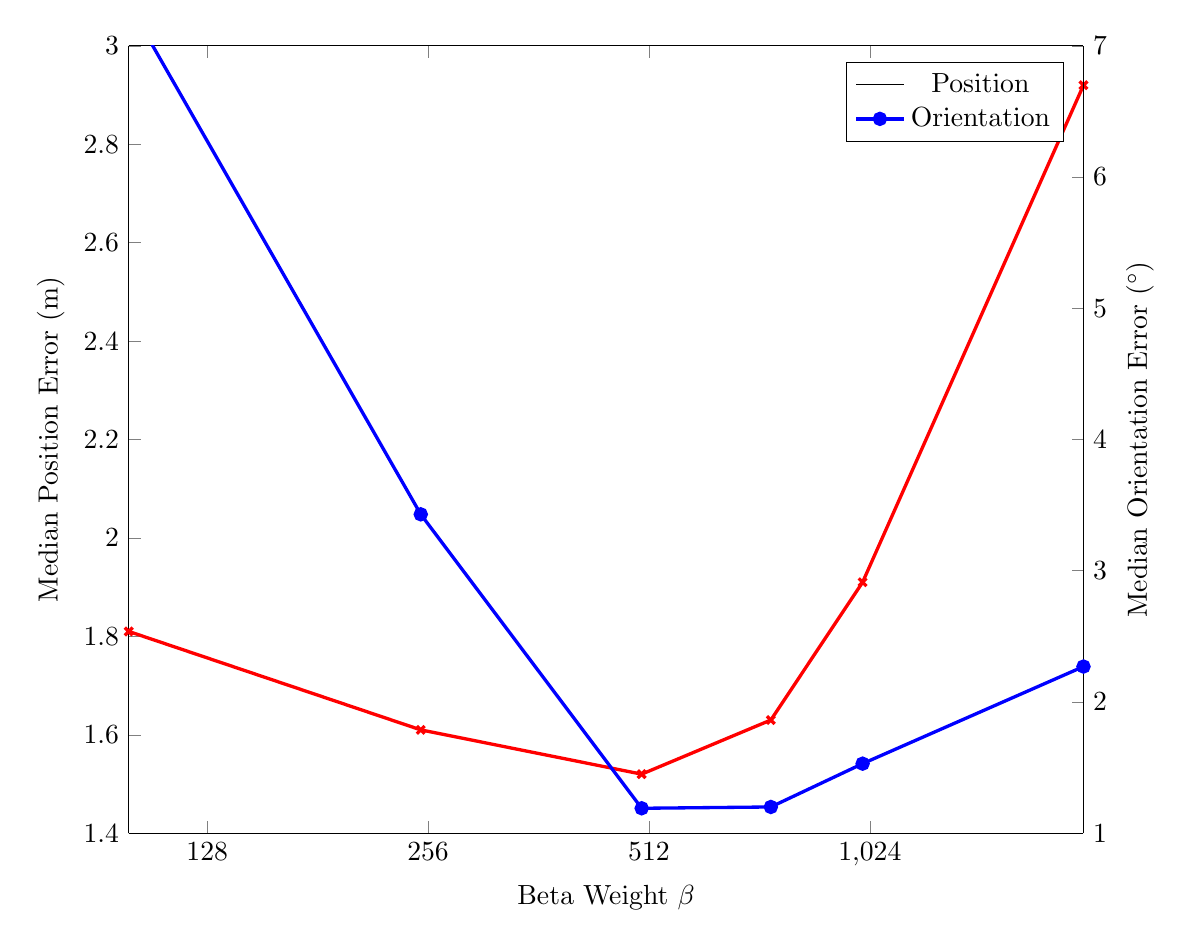
\begin{tikzpicture}
\pgfplotsset{
    compat=1.3,
    scale only axis,
    height=10cm,
    width=\columnwidth %-\widthof{100}-0.1cm, % \textwidth minus width of longest label text minus label offset
    %legend pos =north east,
}

\begin{axis}[
  xmode=log,
  log ticks with fixed point,
  axis y line*=left,
  ymin=1.4, ymax=3.0,
  xlabel=Beta Weight $\beta$,
  ylabel=Median Position Error (m),
  xmin=100, xmax=2000,
    log basis x={2},
    xticklabel=\pgfmathparse{2^\tick}\pgfmathprintnumber{\pgfmathresult},
]
\addplot[mark=x,red,very thick]
  coordinates{
    (100,1.81)
    (250,1.61)
    (500,1.52)
    (750,1.63)
    (1000,1.91)
    (2000,2.92)
}; \label{plot_one1}
\addlegendentry{Position}
\end{axis}

\begin{axis}[
  xmode=log,
  log ticks with fixed point,
  axis y line*=right,
  xtick=\empty,
  ymin=1.0, ymax=7.0,
  ylabel=Median Orientation Error ($\degree$),
  xmin=100, xmax=2000,
]
\addlegendimage{/pgfplots/refstyle=plot_one1}\addlegendentry{Position}
\addplot[mark=*,blue,very thick]
  coordinates{
    (100,7.32)
    (250,3.43)
    (500,1.19)
    (750,1.20)
    (1000,1.53)
    (2000,2.27)
};
\addlegendentry{Orientation}
\end{axis}
\end{tikzpicture}}
 
	\caption[Model performance against a range of scale factors.]{Relative performance of position and orientation regression on \textbf{a single model with a range of scale factors} for an indoor scene from the King's College scene in Cambridge Landmarks, using the loss function in \eqn{loss1}. This demonstrates that learning with the optimum scale factor leads to the network uncovering a more accurate pose function.}
\label{fig:scalefactor}
\end{figure}

\subsubsection{Learning an Optimal Weighting}
\label{sec:learn_loss}

Ideally, we would like a loss function which is able to learn position and orientation optimally, without including any hyper parameters. For this reason, we use the multi-task loss function from \cref{sec:mlttask}, which is able to learn a weighting between the position and orientation objective functions. We formulate it using \textit{homoscedastic uncertainty} which we can learn using probabilistic deep learning \citep{kendall2017uncertainties}. Homoscedastic uncertainty is a measure of uncertainty which does not depend on the input data, as opposed to heteroscedastic uncertainty which is a function of the input data \citep{kendall2017uncertainties}. Rather, it captures the uncertainty of the task itself. In \citep{kendall2017multi} we show how to use this insight to combine losses for different tasks in a probabilistic manner. Here we show how to apply this to learn camera position and orientation (with a Gaussian likelihood):
\begin{equation}
\label{eqn:loss4}
\mathcal{L}_{\sigma}(I) = \mathcal{L}_x(I) \hat{\sigma}_x^{-2} + \log{\hat{\sigma}_x^2} + \mathcal{L}_{q}(I) \hat{\sigma}_q^{-2} + \log{\hat{\sigma}_q^2}
\end{equation}
where we optimise the homoscedastic uncertainties, $\hat{\sigma}_x^2$, $\hat{\sigma}_q^2$, through backpropagation with respect to the loss function. These uncertainties are free scalar values, not model outputs. They represent the homoscedastic (task) noise.

This loss consists of two components; the residual regressions and the uncertainty regularization terms. We learn the variance, $\sigma^2$, implicitly from the loss function. As the variance is larger, it has a tempering effect on the residual regression term; larger variances (or uncertainty) results in a smaller residual loss. The second regularization term prevents the network from predicting infinite uncertainty (and therefore zero loss). As we expect quaternion values to have much smaller values (they are constrained to the unit manifold), their noise, $\sigma_q^2$ should be much smaller than the position noise, $\sigma_x^2$, which can be many meters in magnitude. As $\sigma_q^2$ should be much smaller than $\sigma_x^2$, orientation regression should be weighted much higher than position -- with a similar effect to $\beta$ in \eqn{loss1}.

In practice, we learn $\hat{s}:=\log\hat{\sigma}^2$ because it is more numerically stable \citep{kendall2017multi}:
\begin{equation}
\label{eqn:loss5}
\mathcal{L}_{\sigma}(I) = \mathcal{L}_x(I) \exp (-\hat{s}_x) + \hat{s}_x + \mathcal{L}_{q}(I) \exp (-\hat{s}_q) + \hat{s}_q
\end{equation}
This is more numerically stable than regressing the variance, $\sigma^2$, because the loss avoids a potential division by zero. The exponential mapping also allows us to regress unconstrained scalar values, where $\exp(-s_i)$ is resolved to the positive domain giving valid values for variance. We find that this loss is very robust to our initialisation choice for the homoscedastic task uncertainty values. Only an approximate initial guess is required, we arbitrarily use initial values of $\hat{s}_x=0.0, \hat{s}_q=-3.0$, for all scenes.

\subsubsection{Learning from Geometric Reprojection Error}
\label{sec:reproj}

Perhaps a more desirable loss is one that does not require balancing of rotational and positional quantities at all. Reprojection error of scene geometry is a representation which combines rotation and translation naturally in a single scalar loss \citep{hartley2000}. Reprojection error is given by the residual between 3-D points in the scene projected onto a 2-D image plane using the ground truth and predicted camera pose. It therefore converts rotation and translation quantities into image coordinates. This naturally weights translation and rotation quantities depending on the scene and camera geometry.

To formulate this loss, we first define a function, $\uppi$, which maps a 3-D point, $\mathbf{g}$, to 2-D image coordinates, $(u,v)^T$:
\begin{equation}
\uppi (\mathbf{x},\mathbf{q},\mathbf{g}) \mapsto \begin{pmatrix} u \\ v \end{pmatrix}
\end{equation}
where $\mathbf{x}$ and $\mathbf{q}$ represent the camera position and orientation. This function, $\uppi$, is defined as:
\begin{equation}
\begin{pmatrix} u' \\ v' \\ w' \end{pmatrix} = \mathsf{K} ( \mathsf{R} \mathbf{g} + \mathbf{x}), 
~~\begin{pmatrix} u \\ v \end{pmatrix} = \begin{pmatrix} u'/w' \\ v'/w' \end{pmatrix}
\end{equation}
where $\mathsf{K}$ is the intrinsic calibration matrix of the camera, and $\mathsf{R}$ is the mapping of $\mathbf{q}$ to its $SO(3)$ rotation matrix, $\textbf{q}_{4\times1} \mapsto \mathsf{R}_{3\times3}$.

We formulate this loss by taking the norm of the reprojection error between the predicted and ground truth camera pose. We take the subset, $\mathcal{G'}$, of all 3-D points in the scene, $\mathcal{G}$, which are visible in the image $I$. The final loss \eqn{loss_reproject} is given by the mean of all the residuals from points, $g_i \in \mathcal{G'}$:
\begin{equation}
\mathcal{L}_g(I) = \dfrac{1}{|\mathcal{G}'|} \sum\limits_{g_i \in \mathcal{G}'} \left\lVert \uppi (\mathbf{x},\mathbf{q},\mathbf{g_i}) - \uppi (\mathbf{\hat{x}},\mathbf{\hat{q}},\mathbf{g_i}) \right\rVert_\gamma
\label{eqn:loss_reproject}
\end{equation}
where $\mathbf{\hat{x}}$ and $\mathbf{\hat{q}}$ are the predicted camera poses from PoseNet, with $\mathbf{x}$ and $\mathbf{q}$ the ground truth label, with norm, $\gamma$, which is discussed in \sct{norm}.

Note that because we are projecting 3-D points using both the ground truth and predicted camera pose we can apply any arbitrary camera model, as long as we use the same intrinsic parameters for both cameras. Therefore for simplicity, we set the camera intrinsics, $K$, to the identity matrix -- camera calibration is not required.

This loss implicitly combines rotation and translational quantities into image coordinates. Minimising reprojection error is often the most desirable balance between these quantities for many applications, such as augmented reality. The key advantage of this loss is that it allows the model to vary the weighting between position and orientation, depending on the specific geometry in the training image. For example, training images with geometry which is far away would balance rotational and translational loss differently to images with geometry very close to the camera.

Interestingly, when experimenting with the original weighted loss in \eqn{loss1} we observed that the hyperparameter $\beta$ was an approximate function of the scene geometry. We observed that it was a function of the landmark distance and size in the scene. Our intuition was that the optimal choice for $\beta$ was approximating the reprojection error in the scene geometry. For example, if the scene is very far away, then rotation is more significant than translation and vice versa. This function is not trivial to model for complex scenes with a large number of landmarks. It will vary significantly with each training example in the dataset. By learning with reprojection error we can use our knowledge of the scene geometry more directly to automatically infer this weighting.

Projecting geometry through a projection model is a differentiable operation involving matrix multiplication. Therefore we can use this loss to train our model with stochastic gradient descent. It is important to note that we do not need to know the intrinsic camera parameters to project this 3-D geometry. This is because we apply the same projection to both the model prediction and ground truth measurement, so we can use arbitrary values.

It should be noted that we need to have some knowledge of the scene's geometry in order to have 3-D points to reproject. The geometry is often known; if our data is obtained through structure from motion, RGBD data or other sensory data (see \sct{data}). Only points from the scene which are visible in the image $I$ are used to compute the loss. We also found it was important for numerical stability to ignore points which are projected outside the image bounds.

\begin{table}[t]
	\centering
\begin{subtable}{\linewidth} \centering
	\begin{tabular}{l|ccc}
& \multicolumn{2}{c}{Median Error} & Accuracy \\
Loss function & x [$m$] & q [$\degree$] & $<2m, 5\degree$ [$\%$] \\ \hline \hline
 Linear sum, $\beta=500$ \eqn{loss1} & 1.52 & 1.19 & 65.0\% \\
 Learn weighting with homoscedastic uncertainty \eqn{loss4} & 0.99 & 1.06 & 85.3\% \\ \hline
 Reprojection loss & \multicolumn{3}{c}{does not converge} \\ \hline
 Learn weighting pretraining $\mapsto$ Reprojection loss \eqn{loss_reproject} & 0.88 & 1.04 & 90.3\% \\
	\end{tabular}
    \caption{Cambridge Landmarks, King's College}
\end{subtable}

\begin{subtable}{\linewidth} \centering
	\begin{tabular}{l|ccc}
& \multicolumn{2}{c}{Median Error} & Accuracy \\
Loss function & x [$m$] & q [$\degree$] & $<2m, 5\degree$ [$\%$] \\ \hline \hline
 Linear sum, $\beta=500$ \eqn{loss1} & 13.1 & 4.68 & 30.1\% \\
 Learn weighting with homoscedastic uncertainty \eqn{loss4} & 9.88 & 4.73 & 41.7\% \\ \hline
 Reprojection loss & \multicolumn{3}{c}{does not converge} \\ \hline
 Learn weighting pretraining $\mapsto$ Reprojection loss \eqn{loss_reproject} & 7.90 & 4.40 & 48.6\% \\
	\end{tabular}
    \caption{Dubrovnik 6K}
\end{subtable}
	\caption[Effect of varying loss functions on localisation performance.]{\textbf{Comparison of different loss functions.} We use an $L_1$ distance for the residuals in each loss. \textit{Linear sum} combines position and orientation losses with a constant scaling parameter $\beta$ \citep{kendall2015modelling} and is defined in \eqn{loss1}. Learn weighting is the loss function in \eqn{loss4} which learns to combine position and orientation using homoscedastic uncertainty. Reprojection error implicitly combines rotation and translation by using the reprojection error of the scene geometry as the loss \eqn{loss_reproject}. We find that homoscedastic uncertainty is able to learn an effective weighting between position and orientation quantities. The reprojection loss was not able to converge from random initialisation. However, when used to fine-tune a network pretrained with \eqn{loss4} it yields the best results.}
	\label{tbl:losses}
\end{table}

\subsubsection{Regression Norm}
\label{sec:norm}

An important choice for these losses is the regression norm, $\left\lVert~\right\rVert_\gamma$. Typically, deep learning models use an $L_1 = \left\lVert~\right\rVert_1$ or $L_2 = \left\lVert~\right\rVert_2$. We can also use robust norms such as Huber's loss \citep{huber2011robust} and Tukey's loss \citep{hoaglin1983understanding}, which have been successfully applied to deep learning \citep{belagiannis2015robust}. For camera pose regression, we found that they negatively impacted performance by over-attenuating difficult examples. We suspect that for more noisy datasets these robust regression functions might be beneficial. With the datasets used in this chapter, we found the $L_1$ norm to perform best and therefore use use $\gamma=1$. It does not increase quadratically with magnitude or over-attenuate large residuals.

\section{Localisation Experiments}
\label{sec:exp}

To train and benchmark our model on a number of datasets we rescale the input images such that the shortest side is of length 256. We normalise the images so that input pixel intensities range from $-1$ to $1$. We train our PoseNet architecture using an implementation in TensorFlow \citep{abadi2016tensorflow}. All models are optimised end-to-end with ADAM \citep{kingma2014adam} using the default parameters and a learning rate of $1 \times 10^{-4}$. We train each model until the training loss converges. We use a batch size of 64 on a NVIDIA Titan X (Pascal) GPU, training takes approximately 20k - 100k iterations, or 4 hours - 1 day.

\subsection{Datasets}
\label{sec:data}

\begin{figure}[p]
\centering

	\begin{subfigure}[t]{\linewidth}
	\resizebox{\linewidth}{!}{
		\includegraphics[width=0.2\linewidth]{Datasets/chess.png}
		\includegraphics[width=0.2\linewidth]{Datasets/fire.png}
		\includegraphics[width=0.2\linewidth]{Datasets/kitchen.png}
		\includegraphics[width=0.2\linewidth]{Datasets/office.png}
		\includegraphics[width=0.2\linewidth]{Datasets/stairs.png}
		}
	\caption{7 Scenes Dataset - 43,000 images from seven scenes in small indoor environments \citep{shotton2013scene}.}
	~
	~
	\end{subfigure}
	
	\begin{subfigure}[t]{\linewidth}
	\resizebox{\linewidth}{!}{
		\includegraphics[width=0.2\linewidth]{Datasets/frame00015.jpg}
		\includegraphics[width=0.2\linewidth]{Datasets/frame00016.jpg}
		\includegraphics[width=0.2\linewidth]{Datasets/frame00428.jpg}
		\includegraphics[width=0.2\linewidth]{Datasets/frame00599.jpg}
		\includegraphics[width=0.2\linewidth]{Datasets/frame00615.jpg}
		}
        
    \vspace{0.5mm}
	\resizebox{\linewidth}{!}{
		\includegraphics[width=0.2\linewidth]{Datasets/image1_000031.jpg}
		\includegraphics[width=0.2\linewidth]{Datasets/image2_000585.jpg}
		\includegraphics[width=0.2\linewidth]{Datasets/image2_001336.jpg}
		\includegraphics[width=0.2\linewidth]{Datasets/image2_001351.jpg}
		\includegraphics[width=0.2\linewidth]{Datasets/image2_002421.jpg}
		}
	\caption{Cambridge Landmarks Dataset - over 10,000 images from six scenes around Cambridge, UK \citep{kendall2015posenet}.}
	~
	~
	\end{subfigure}
	
	\begin{subfigure}[t]{\linewidth}
	\resizebox{\linewidth}{!}{
		\includegraphics[height=50mm]{Datasets/5n4k3_2760651317.jpg}
		\includegraphics[height=50mm]{Datasets/5pointloperist_2921626253.jpg}
		\includegraphics[height=50mm]{Datasets/709913_2965924825.jpg}
		\includegraphics[height=50mm]{Datasets/7145465_N07_3065208814.jpg}
		\includegraphics[height=50mm]{Datasets/7286581_N04_2243494109.jpg}
		}
        
    \vspace{0.5mm}
	\resizebox{\linewidth}{!}{
		\includegraphics[height=50mm]{Datasets/8117903_N06_2955594865.jpg}
		\includegraphics[height=50mm]{Datasets/8117903_N06_2956436946.jpg}
		\includegraphics[height=50mm]{Datasets/8223442_N02_3167519460.jpg}
		\includegraphics[height=50mm]{Datasets/10970812_N05_2553025324.jpg}
		\includegraphics[height=50mm]{Datasets/16798538_N06_1808716980.jpg}
		}
	\caption{Dubrovnik 6K Dataset - 6,000 images from a variety of camera types in Dubrovnik, Croatia \citep{li2010location}.}
	~
	~
	\end{subfigure}
	
\caption[Localisation datasets.]{\textbf{Example images randomly chosen from each dataset.} This illustrates the wide variety of settings and scales and the challenging array of environmental factors such as lighting, occlusion, dynamic objects and weather which are captured in each dataset.}
\label{fig:datasets}
\end{figure}


\afterpage{%
    \clearpage% Flush earlier floats (otherwise order might not be correct)
    \begin{landscape}% Landscape page
    \centering
\begin{table*}[t]
	\centering
	\resizebox{\linewidth}{!}{
	\begin{tabular}{l|c|c|c|c|c|c|c|c}
		Dataset & Type & Scale & Imagery & Scenes & Train Images & Test Images & 3-D Points & Spatial Area \\ \hline \hline
		7 Scenes & Indoor & Room & RGB-D sensor (Kinect) & 7 & 26,000 & 17,000 & - & 4$\times$3m \\
		Cambridge Landmarks & Outdoor & Street & Mobile phone camera & 6 & 8,380 & 4,841 & 2,097,191 & 100$\times$500m \\
		Dubrovnik 6K & Outdoor & Small town & Internet images (Flikr) & 1 & 6,044 & 800 & 2,106,456 & 1.5$\times$1.5km \\
		%San Francisco (SF1) & Outdoor & Large city & Vehicle camera & 1 & 790,000 & 800 & 75,410,077 & 4$\times$4km\\
	\end{tabular}}
	\caption[Localisation dataset details.]{\textbf{Summary of the localisation datasets used in this chapter's experiments.} We compare 7 Scenes \citep{shotton2013scene}, Cambridge Landmarks \citep{kendall2015posenet}, Dubrovnik \citep{li2012worldwide} and the San Francisco \citep{chen2011city} datasets. These datasets are all publicly available. They demonstrate our method's performance over a range of scales for both indoor and outdoor applications.}
	\label{tbl:datasets}
\end{table*}
\end{landscape}
\clearpage% Flush page
}

Deep learning performs extremely well on large datasets. However annotating ground truth labels on these datasets is often expensive or very labour intensive. We can leverage structure from motion \citep{Snavely08IJCV}, or similar algorithms \citep{shotton2013scene}, to autonomously generate training labels (camera poses) from image data \citep{kendall2015posenet}. We use three datasets to benchmark our approach. These datasets are summarised in \tbl{datasets} and example imagery is shown in \fig{datasets}. We use these datasets to demonstrate our method's performance across a range of settings and scales. We endeavour to demonstrate the general applicability of the approach.

\textbf{Cambridge Landmarks} \citep{kendall2015posenet} provides labelled video data to train and test pose regression algorithms in an outdoor urban setting. It was collected using a smart phone and structure from motion was used to generate the pose labels \citep{wu2013towards}. Significant urban clutter such as pedestrians and vehicles were present and data was collected from many different points in time representing different lighting and weather conditions. Train and test images are taken from distinct walking paths and not sampled from the same trajectory making the regression challenging.

\textbf{7 Scenes} \citep{shotton2013scene} is an indoor dataset which was collected with a Kinect RGB-D sensor. Ground truth poses were computed using Kinect Fusion \citep{shotton2013scene}. The dataset contains seven scenes which were captured around an office building. Each scene typically consists of a single room. The dataset was originally created for RGB-D relocalisation. It is extremely challenging for purely visual relocalisation using SIFT-like features, as it contains many ambiguous textureless features.

\textbf{Dubrovnik 6K} \citep{li2012worldwide} is a dataset consisting of 6,044 train and 800 test images which were obtained from the internet. They are taken from Dubrovnik's old town in Croatia which is a UNESCO world heritage site. The images are predominantly captured by tourists with a wide variety of camera types. Ground truth poses for this dataset were computed using structure from motion.

\subsection{Comparison of Loss Functions}
\label{sec:loss_exp}

In \tbl{losses} we compare different combinations of losses and regression norms. We compare results for a scene in the Cambridge Landmarks dataset \citep{kendall2015posenet} and the Dubrovnik 6K dataset \citep{li2012worldwide}, which has imagery from a range of cameras.

We find that modelling homoscedastic uncertainty with the loss in \eqn{loss4} is able to effectively learn a weighting between position and orientation. It outperforms the constant weighting used in loss \eqn{loss1}. The reprojection loss in \eqn{loss_reproject} is unable to train the model from a random initialisation. We observe that the model gets stuck in a poor local minima, when using any of the regression norms. However, the reprojection loss is able to improve localisation performance when using weights pretrained with any of the other losses. For example, we can take the best performing model using the loss from \eqn{loss4} and fine tune with the reprojection loss \eqn{loss_reproject}. We observe that this loss is then able to converge effectively. This shows that the reprojection loss is not robust to large residuals. This is because reprojected points can be easily placed far from the image centre if the network makes a poor pose prediction. Therefore, we recommend the following two-step training scheme:
\begin{enumerate}
  \item Train the model using the loss in \eqn{loss4}, learning the weighting between position and orientation.
  \item If the scene geometry is known (for example from structure from motion or RGBD camera data) then fine-tune the model using the reprojection loss in \eqn{loss_reproject}.
\end{enumerate}

\afterpage{%
    \clearpage% Flush earlier floats (otherwise order might not be correct)
    \begin{landscape}% Landscape page
    \centering
\begin{table*}[t]
\begin{center}
	\resizebox{\linewidth}{!}{
\begin{tabular}{l|c|c c c c c c}
 & Area or & Active Search (SIFT) & PoseNet ($\beta$ weight) & Bayesian PoseNet & PoseNet Spatial LSTM & PoseNet & PoseNet\\
Scene & Volume & \citep{sattler2016efficient} & \citep{kendall2015posenet} & \citep{kendall2015modelling} &  \citep{walch2016image} & Learn $\sigma^2$ Weight & Geometric Reprojection\\
\hline \hline
Great Court	 		& $8000m^2$		& -- 				 &	--				  &	--			   	   & -- 				& 7.00m, 3.65\degree & 6.83m, 3.47\degree \\
King's College 		& $5600m^2$ 	& 0.42m, 0.55\degree & 1.66m, 4.86\degree & 1.74m, 4.06\degree & 0.99m, 3.65\degree & 0.99m, 1.06\degree & 0.88m, 1.04\degree \\
Old Hospital 		& $2000m^2$ 	& 0.44m, 1.01\degree & 2.62m, 4.90\degree & 2.57m, 5.14\degree & 1.51m, 4.29\degree & 2.17m, 2.94\degree & 3.20m, 3.29\degree \\
Shop Fa\c cade 		& $875m^2$ 		& 0.12m, 0.40\degree & 1.41m, 7.18\degree & 1.25m, 7.54\degree & 1.18m, 7.44\degree & 1.05m, 3.97\degree & 0.88m, 3.78\degree \\
St Mary's Church 	& $4800m^2$ 	& 0.19m, 0.54\degree & 2.45m, 7.96\degree & 2.11m, 8.38\degree & 1.52m, 6.68\degree & 1.49m, 3.43\degree & 1.57m, 3.32\degree \\
Street 				& $50000m^2$ 	& 0.85m, 0.83\degree & -- 				  & -- 				   & --					& 20.7m, 25.7\degree & 20.3m, 25.5\degree \\
\hline
\multicolumn{5}{c}{}\\
\hline
Chess 		& $6m^3$ 	& 0.04m, 1.96\degree & 0.32m, 6.60\degree & 0.37m, 7.24\degree & 0.24m, 5.77\degree & 0.14m, 4.50\degree & 0.13m, 4.48\degree \\
Fire 		& $2.5m^3$ 	& 0.03m, 1.53\degree & 0.47m, 14.0\degree & 0.43m, 13.7\degree & 0.34m, 11.9\degree & 0.27m, 11.8\degree & 0.27m, 11.3\degree \\
Heads 		& $1m^3$ 	& 0.02m, 1.45\degree & 0.30m, 12.2\degree & 0.31m, 12.0\degree & 0.21m, 13.7\degree & 0.18m, 12.1\degree & 0.17m, 13.0\degree \\
Office 		& $7.5m^3$ 	& 0.09m, 3.61\degree & 0.48m, 7.24\degree & 0.48m, 8.04\degree & 0.30m, 8.08\degree & 0.20m, 5.77\degree & 0.19m, 5.55\degree \\
Pumpkin 	& $5m^3$ 	& 0.08m, 3.10\degree & 0.49m, 8.12\degree & 0.61m, 7.08\degree & 0.33m, 7.00\degree & 0.25m, 4.82\degree & 0.26m, 4.75\degree \\
Red Kitchen & $18m^3$	& 0.07m, 3.37\degree & 0.58m, 8.34\degree & 0.58m, 7.54\degree & 0.37m, 8.83\degree & 0.24m, 5.52\degree & 0.23m, 5.35\degree \\
Stairs 		& $7.5m^3$ 	& 0.03m, 2.22\degree & 0.48m, 13.1\degree & 0.48m, 13.1\degree & 0.40m, 13.7\degree & 0.37m, 10.6\degree & 0.35m, 12.4\degree \\
\hline
\end{tabular}}
\end{center}

	\caption[Localisation results for Cambridge Landmarks and 7 Scenes.]{\textbf{Median localisation results for the \textit{Cambridge Landmarks} \citep{kendall2015posenet} and \textit{7 Scenes} \citep{shotton2013scene} datasets.} We compare the performance of various RGB-only algorithms. Active search \citep{sattler2016efficient} is a state-of-the-art traditional SIFT keypoint based baseline. We demonstrate a notable improvement over PoseNet's \citep{kendall2015posenet} baseline performance using the learned $\sigma^2$ and reprojection error proposed in this chapter, narrowing the margin to the state of the art SIFT technique.}
	\label{tbl:mainresults}
\end{table*}
\end{landscape}
\clearpage% Flush page
}

\subsection{Benchmarking Localisation Accuracy}
\label{sec:benchmark}

In \tbl{mainresults} we show that our geometry based loss outperforms the original PoseNet's naive loss function \citep{kendall2015posenet}. We observe a consistent and significant improvement across both indoor \textit{7 Scenes} outdoor \textit{Cambridge Landmarks} datasets. We conclude that we can simultaneously learn both position and orientation more effectively by considering scene geometry. The improvement is notably more pronounced for the 7Scenes dataset. We believe this is due to the significantly larger amount of training data for each scene in this dataset, compared with Cambridge Landmarks. We also outperform the improved PoseNet architecture with spatial LSTMs \citep{walch2016image}. However, this method is complimentary to the loss functions in this chapter, and it would be interesting to explore the union of these ideas.

We observe a difference in relative performance between position and orientation when optimising with respect to reprojection error \eqn{loss_reproject} or homoscedastic uncertainty \eqn{loss4}. Overall, optimising reprojection loss improves rotation accuracy, sometimes at the expense of some positional precision.

\subsection{Comparison to SIFT-Feature Approaches}

\tbl{mainresults} also compares to a state-of-the-art traditional SIFT feature based localisation algorithm, Active Search \citep{sattler2016efficient}. This method outperforms PoseNet, and is effective in feature-rich outdoor environments. However, in the 7Scenes dataset this deficit is less pronounced. The indoor scenes contain much fewer point features and there is significantly more training data. As an explanation for the deficit in these results, PoseNet only uses $256\times 256$ pixel images, while SIFT based methods require images of a few mega-pixels in size \citep{sattler2016efficient}. Additionally, PoseNet is able to localise an image in $5ms$, scaling constantly with scene area, while traditional SIFT feature approaches require over $100ms$, and scale with scene size \citep{sattler2016efficient}.

In \tbl{dubrovnik_results} we compare our approach on the Dubrovnik dataset to other geometric techniques which localise by registering SIFT features \citep{lowe2004distinctive} to a large 3-D model \citep{li2012worldwide}. Although our method improves significantly over the original PoseNet model, it is still yet to reach the fine grained accuracy of these methods \citep{svarm2014accurate,zeisl2015camera,sattler2011fast,li2010location}. We hypothesise that this is due to a lack of training data, with only 6k images across the town. However, our algorithm is significantly faster than these approaches. Furthermore, it is worth noting that PoseNet only sees a $256\times256$ resolution image, while these methods register the full size images, often with a few million pixels.
	
\begin{table}[t]
	\centering
	\begin{tabular}{l|cc|cc}
		& \multicolumn{2}{c|}{Position} & \multicolumn{2}{c}{Orientation} \\
		Method & Mean [m] & Median [m] & Mean [$\degree$] & Median [$\degree$] \\ \hline \hline
		PoseNet (this work) & 40.0 & 7.9 & 11.2 & 4.4 \\
		APE \citep{svarm2014accurate} & - & 0.56 & - & - \\
		Voting \citep{zeisl2015camera} & - & 1.69 & - & - \\
		Sattler, et al. \citep{sattler2011fast} & 14.9 & 1.3 & - & - \\
		P2F \citep{li2010location} & 18.3 & 9.3 & - & - \\
	\end{tabular}
	\caption[Localisation results for the Dubrovnik dataset.]{\textbf{Localisation results on the Dubrovnik dataset} \citep{li2012worldwide}, comparing to a number of state-of-the-art point-feature techniques. Our method is the first deep learning approach to benchmark on this challenging dataset. We achieve comparable performance, while our method only requires a 256$\times$256 pixel image and is much faster to compute.}
	\label{tbl:dubrovnik_results}
\end{table}




\begin{figure}[t]
   	\includegraphics[width=\linewidth]{ICCV/zoominmap}
   \caption[Localisation results over train and test sequences.]{Magnified view of a sequence of \textbf{training (green)} and \textbf{testing (blue)} cameras for King's College. We show the \textbf{predicted camera pose in red} for each testing frame. The images show the test image (top), the predicted view from our model overlaid in red on the input image (middle) and the nearest neighbour training image overlaid in red on the input image (bottom). This shows our system can interpolate camera pose effectively in space between training frames.}
\label{fig:zoommap}
\end{figure}

\begin{figure}[t]
\makebox[\textwidth][c]{
   	\includegraphics[height=0.2\linewidth]{ICCV/kingsmap}
   	~
   	\includegraphics[height=0.2\linewidth]{ICCV/kpmap}
   	~
   	\includegraphics[height=0.2\linewidth]{ICCV/jbsmap}
   	~
   	\includegraphics[height=0.2\linewidth]{ICCV/ramap}
   	~
   	\includegraphics[height=0.2\linewidth]{ICCV/stmarysmap}
   	}
\makebox[\textwidth][l]{
\makebox[0.44\textwidth][c]{
\textit{King's College}
   	}
\makebox[0.03\textwidth][c]{
\textit{Street}
   	}
\makebox[0.24\textwidth][c]{
\textit{Old Hospital}
   	}
\makebox[0.1\textwidth][c]{
\textit{Shop Fa\c cade}
   	}
\makebox[0.2\textwidth][c]{
\textit{St Mary's Church}
   	}}
   \caption[Map of Cambridge Landmarks dataset.]{\textbf{Map of dataset} showing training frames (green), testing frames (blue) and their predicted camera pose (red). The testing sequences are distinct trajectories from the training sequences and each scene covers a very large spatial extent.}
   \label{fig:map}
\end{figure}






\begin{figure}[p]
\clearpage% Flush page
\begin{center}
\vspace{-7mm}
\begin{subfigure}[b]{\textwidth}
\makebox[\textwidth][c]{
   	\includegraphics[width=0.16\linewidth]{ICCV/kings_seq3_frame00110_blur25}
   	\includegraphics[width=0.16\linewidth]{ICCV/kings_seq3_frame00110_blur50}
   	\includegraphics[width=0.16\linewidth]{ICCV/kings_seq3_frame00110_blur100}
   	\includegraphics[width=0.16\linewidth]{ICCV/kings_seq7_frame00010_blur25}
   	\includegraphics[width=0.16\linewidth]{ICCV/kings_seq7_frame00010_blur50}
   	\includegraphics[width=0.16\linewidth]{ICCV/kings_seq7_frame00010_blur100}
   	}
\makebox[\textwidth][c]{
   	\includegraphics[width=0.16\linewidth]{ICCV/king_seq3_frame00110_blur25pngscreenshot}
   	\includegraphics[width=0.16\linewidth]{ICCV/king_seq3_frame00110_blur50pngscreenshot}
   	\includegraphics[width=0.16\linewidth]{ICCV/king_seq3_frame00110_blur100pngscreenshot}
   	\includegraphics[width=0.16\linewidth]{ICCV/king_seq7_frame00010_blur25pngscreenshot}
   	\includegraphics[width=0.16\linewidth]{ICCV/king_seq7_frame00010_blur50pngscreenshot}
   	\includegraphics[width=0.16\linewidth]{ICCV/king_seq7_frame00010_blur100pngscreenshot}
   	}
   \caption{Relocalisation with increasing levels of motion blur. The system is able to recognize the pose as high level features such as the contour outline still exist. Blurring the landmark increases apparent contour size and the system believes it is closer. }
\end{subfigure}

\begin{subfigure}[b]{\textwidth}
\makebox[\textwidth][c]{
   	\includegraphics[width=0.24\linewidth]{ICCV/frame00023}
   	\includegraphics[width=0.24\linewidth]{ICCV/frame00048}
   	\includegraphics[width=0.24\linewidth]{ICCV/frame00054}
   	\includegraphics[width=0.24\linewidth]{ICCV/IMG_20150418_230453}
   	}
\makebox[\textwidth][c]{
   	\includegraphics[width=0.24\linewidth]{ICCV/fram00023pngscreenshot}
   	\includegraphics[width=0.24\linewidth]{ICCV/fram00048pngscreenshot}
   	\includegraphics[width=0.24\linewidth]{ICCV/fram00054pngscreenshot}
   	\includegraphics[width=0.24\linewidth]{ICCV/IMG_20150418_230453jpgscreenshot}
   	}
\makebox[\textwidth][c]{
   	\includegraphics[width=0.24\linewidth]{ICCV/fram00023pngoverlay}
   	\includegraphics[width=0.24\linewidth]{ICCV/fram00048pngoverlay}
   	\includegraphics[width=0.24\linewidth]{ICCV/fram00054pngoverlay}
   	\includegraphics[width=0.24\linewidth]{ICCV/IMG_20150418_230453jpgoverlay}
   	}
   \caption{Relocalisation under difficult dusk and night lighting conditions. In the dusk sequences, the landmark is silhouetted against the backdrop however again the model seems to recognize the contours and estimate pose.}
\end{subfigure}

\vspace{-5mm}
\begin{subfigure}[t]{0.28\textwidth}
\makebox[\textwidth][c]{
   	\includegraphics[width=0.5\textwidth]{ICCV/frame00029}
   	\includegraphics[width=0.5\textwidth]{ICCV/frame00060}
   	}
\makebox[\textwidth][c]{
   	\includegraphics[width=0.5\textwidth]{ICCV/fram00029pngscreenshot}
   	\includegraphics[width=0.5\textwidth]{ICCV/fram00060pngscreenshot}
   	}
\makebox[\textwidth][c]{
   	\includegraphics[width=0.5\textwidth]{ICCV/fram00029pngoverlay}
   	\includegraphics[width=0.5\textwidth]{ICCV/fram00060pngoverlay}
   	}
   \caption{Relocalisation with different weather conditions. PoseNet is able to effectively estimate pose in fog and rain.}
\end{subfigure}
\qquad
\begin{subfigure}[t]{0.28\textwidth}
\makebox[\textwidth][c]{
   	\includegraphics[width=0.5\textwidth]{ICCV/frame00037}
   	\includegraphics[width=0.5\textwidth]{ICCV/frame00008}
   	}
\makebox[\textwidth][c]{
   	\includegraphics[width=0.5\textwidth]{ICCV/seq2frame00037pngscreenshot}
   	\includegraphics[width=0.5\textwidth]{ICCV/seq1frame00008pngscreenshot}
   	}
\makebox[\textwidth][c]{
   	\includegraphics[width=0.5\textwidth]{ICCV/seq2frame00037pngoverlay}
   	\includegraphics[width=0.5\textwidth]{ICCV/seq1frame00008pngoverlay}
   	}
   \caption{Relocalisation with significant people, vehicles and other dynamic objects.}
\end{subfigure}
\qquad
\begin{subfigure}[t]{0.28\textwidth}
\makebox[\textwidth][c]{
   	\includegraphics[width=0.5\textwidth]{ICCV/img1}
   	\includegraphics[width=0.5\textwidth]{ICCV/frame00051}
   	}
\makebox[\textwidth][c]{
   	\includegraphics[width=0.5\textwidth]{ICCV/img1jpgscreenshot}
   	\includegraphics[width=0.5\textwidth]{ICCV/seq2frame00051pngscreenshot}
   	}
\makebox[\textwidth][c]{
   	\includegraphics[width=0.5\textwidth]{ICCV/img1jpgoverlay}
   	\includegraphics[width=0.5\textwidth]{ICCV/seq2frame00051pngoverlay}
   	}
   \caption{Relocalisation with unknown camera intrinsics: SLR with focal length 45mm (left), and iPhone 4S with focal length 35mm (right) compared to the dataset's camera which had a focal length of 30mm.}
\end{subfigure}
\end{center}
\vspace{-5mm}
	\caption[Robustness to challenging real life situations.]{\textbf{Robustness to challenging real life situations.} Registration with point based techniques such as SIFT fails in examples (a-c), therefore ground truth measurements are not available. None of these types of challenges were seen during training. As convolutional neural networks are able to understand objects and contours they are still successful at estimating pose from the building's contour in the silhouetted examples (b) or even under extreme motion blur (a). Many of these quasi invariances were enhanced by pretraining from the scenes dataset.}
	\label{fig:difficultexamples}
\clearpage% Flush page
\end{figure}

We show that PoseNet is able to effectively localize across both the indoor \textit{7 Scenes} dataset and outdoor \textit{Cambridge Landmarks} dataset in \cref{tbl:mainresults}. To validate that the model is regressing pose beyond that of the training examples we show the performance for finding the nearest neighbour representation in the training data from the feature vector produced by the localisation network. As our performance exceeds this we conclude that the network is successfully able to regress pose beyond training examples (see \cref{fig:zoommap}). We also compare our algorithm to the RGB-D SCoRe Forest algorithm \citep{shotton2013scene}. 

\begin{figure*}[t]
\makebox[\textwidth][c]{
   	\includegraphics[width=0.26\linewidth]{ICCV/kings}
   	\includegraphics[width=0.26\linewidth]{ICCV/businessschool}
   	\includegraphics[width=0.26\linewidth]{ICCV/pumpkin}
   	\includegraphics[width=0.26\linewidth]{ICCV/stairs}
   	}
   \caption[Localisation histograms.]{\textbf{Localization performance.} These figures show our localization accuracy for both position and orientation as a cumulative histogram of errors for the entire training set. The regression network outperforms the nearest neighbour feature matching which demonstrates we regress finer resolution results than given by training. Comparing to the RGB-D SCoRe Forest approach shows that our method is competitive, but outperformed by a more expensive depth approach. Our method does perform better on the hardest few frames, above the 95th percentile, with our worst error lower than the worst error from the SCoRe approach. }
   \label{fig:histograms}
\end{figure*}

\cref{fig:histograms} shows cumulative histograms of localisation error for two indoor and two outdoor scenes. We note that although the SCoRe forest is generally more accurate, it requires depth information, and uses higher-resolution imagery. The indoor dataset contains many ambiguous and textureless features which make relocalisation without this depth modality extremely difficult. We note our method often localizes the most difficult testing frames, above the 95th percentile, more accurately than SCoRe across all the scenes. We also observe that dense cropping only gives a modest improvement in performance. It is most important in scenes with significant clutter like pedestrians and cars, for example King's College, Shop Fa\c cade and St Mary's Church.

We explored the robustness of this method beyond what was tested in the dataset with additional images from dusk, rain, fog, night and with motion blur and different cameras with unknown intrinsics. \cref{fig:difficultexamples} shows the convolutional neural network generally handles these challenges well. SfM with SIFT fails in all these cases so we were not able to generate a ground truth camera pose, however we infer the accuracy by viewing the 3-D reconstruction from the predicted camera pose, and overlaying this onto the input image.

\subsection{Robustness Against Training Image Spacing}

We demonstrate in \cref{fig:baseline} that, for an outdoor scale scene, we gain little by spacing the training images more closely than 4m. The system is robust to very large spatial separation between training images, achieving reasonable performance even with only a few dozen training samples. The pose accuracy deteriorates gracefully with increased training image spacing, whereas SIFT-based SfM sharply fails after a certain threshold as it requires a small baseline \citep{lowe2004distinctive}.

\begin{figure}[t]
\begin{center}
   	\includegraphics[width=0.7\linewidth]{ICCV/reduced_baseline}
\end{center}
   \caption[Robustness to a decreasing training baseline.]{\textbf{Robustness to a decreasing training baseline} for the King's College scene. Our system exhibits graceful decline in performance as fewer training samples are used.}
\label{fig:baseline}
\end{figure}

\subsection{Importance of Transfer Learning}

In general deep networks require large amounts of training data. We sidestep this problem by starting our pose training from a network pretrained on giant datasets such as \textit{ImageNet} and \textit{Places}. Similar to what has been demonstrated for classification tasks, \cref{fig:transfer} shows how transfer learning can be utilised effectively between classification and complicated regression tasks. Such `transfer learning' has been demonstrated elsewhere for training classifiers \citep{razavian2014cnn,oquab2014learning,bengio2013representation}, but here we demonstrate transfer learning from classification to the qualitatively different task of pose regression. It is not immediately obvious that a network trained to output pose-invariant classification labels would be suitable as a starting point for a pose regressor. We find, however, that this is not a problem in practice. A possible explanation is that, in order for its output to be invariant to pose, the classifier network must keep track of pose, to better factor its effects away from identity cues. This would agree with our own findings that a network trained to output position and orientation outperforms a network trained to output only position. By preserving orientation information in the intermediate representations, it is better able to factor the effects of orientation out of the final position estimation. Transfer learning gives not only a large improvement in training speed, but also end performance. 

The relevance of data is also important. In \cref{fig:transfer} the \textit{Places} and \textit{ImageNet} curves initially have the same performance. However, ultimately the \textit{Places} pretraining performs better due to being a more relevant dataset to this localisation task.

\begin{figure}[t]
\begin{center}
   	\adjustbox{trim={0} {0} {0} {0.05\height},clip}{\includegraphics[width=0.9\linewidth]{ICCV/transferlearning.pdf}}
\end{center}
   \caption[Importance of transfer learning.]{\textbf{Importance of transfer learning.} Shows how pretraining on large datasets gives an increase in both performance and training speed.}
\label{fig:transfer}
\end{figure}

\subsection{Visualising Features Relevant to Pose}

\begin{figure*}[t]
\makebox[\linewidth][c]{
   	\includegraphics[width=0.33\linewidth]{ICCV/img_com2_wpqr}
   	\includegraphics[width=0.33\linewidth]{ICCV/img_com7_xyz_kings}
   	\includegraphics[width=0.33\linewidth]{ICCV/img_com5_wpqr}
   	}
   \caption[Saliency maps.]{\textbf{Saliency maps.} This figure shows the saliency map superimposed on the input image. The saliency maps suggest that the convolutional neural network exploits not only distinctive point features (\`{a} la SIFT), but also large textureless patches, which can be as informative, if not more so, to the pose. This, combined with a tendency to disregard dynamic objects such as pedestrians, enables it to perform well under challenging circumstances. (Best viewed electronically.)}
\label{fig:saliency}
\end{figure*}

\cref{fig:saliency} shows example saliency maps produced by PoseNet. The saliency map, as used in \citep{simonyan2013deep}, is the magnitude of the gradient of the loss function with respect to the pixel intensities. This uses the sensitivity of the pose with respect to the pixels as an indicator of how important the network considers different parts of the image.

These results show that the strongest response is observed from higher-level features such as windows and spires. However a more surprising result is that PoseNet is also very sensitive to large textureless patches such as road, grass and sky. These textureless patches may be more informative than the highest responding points because the effect of a group of pixels on the pose variable is the sum of the saliency map values over that group of pixels. This evidence points to the net being able to localize off information from these textureless surfaces, something which interest-point based features such as SIFT or SURF fail to do.

The last observation is that PoseNet has an attenuated response to people and other noisy objects, effectively masking them. These objects are dynamic, and the model has identified them as not appropriate for localisation.

\subsection{Viewing the Internal Representation}

\begin{figure}[t]
\makebox[\linewidth][c]{
   	\framebox[\width]{ \includegraphics[width=0.35\linewidth]{ICCV/tsne_places_googlenet_on_kings_seq3}}
   	\framebox[\width]{ \includegraphics[width=0.35\linewidth]{ICCV/tsne_kingsparade_googlenet_on_kings_seq3}}
   	\framebox[\width]{ \includegraphics[width=0.35\linewidth]{ICCV/tsne_kings_googlenet_on_kings_seq3}}
   	}
\makebox[\linewidth][c]{
\makebox[0.35\linewidth][c]{
(a)
   	}
\makebox[0.35\linewidth][c]{
(b)
   	}
\makebox[0.35\linewidth][c]{
(c)
   	}}
   \caption[Feature vector visualisation.]{\textbf{Feature vector visualisation.} t-SNE visualisation of the feature vectors from a video sequence traversing an outdoor scene (King's College) in a straight line. Colour represents time. The feature representations are generated from the model with weights trained on \textit{Places} (a), \textit{Places} then another outdoor scene, St Mary's Church (b), \textit{Places} then this outdoor scene, King's College (c). Despite (a,b) not being trained on this scene, these visualizations suggest that it is possible to compute the pose as a simple, if non-linear, function of these representations.}
\label{fig:tsne}
\end{figure}

t-SNE \citep{van2008visualizing} is an algorithm for embedding high-dimensional data in a low dimensional space, in a way that tries to preserve Euclidean distances. It is often used, as we do here, to visualize high-dimensional feature vectors in two dimensions. In \cref{fig:tsne} we apply t-SNE to the feature vectors computed from a sequence of video frames taken by a pedestrian. As these figures show, the feature vectors are a function that smoothly varies with, and is largely one-to-one with, pose. This `pose manifold' can be observed not only on networks trained on other scenes, but also networks trained on classification image sets without pose labels. This further suggests that classification networks preserve pose information up to the final layer, regardless of whether it's expressed in the output. However, the mapping from feature vector to pose becomes more complicated for networks not trained on pose data. Furthermore, as this manifold exists on scenes that the model was not trained on, the model must learn some generic representation of the relationship between landmarks, geometry and camera motion. This demonstrates that the feature vector that is produced from regression is able to generalize to other tasks in the same way as classification networks.

\subsection{System Efficiency}

\begin{figure}[t]
\makebox[\linewidth][c]{
   	%\includegraphics[width=\linewidth]{ICCV/speedmemory-eps-converted-to.pdf}
   	}
   \caption[Implementation efficiency.]{\textbf{Implementation efficiency.} Experimental speed and memory use of the regression network, nearest neighbour network feature vector baseline and SIFT relocalisation methods.}
\label{fig:speed}
\end{figure}

\cref{fig:speed} compares system performance of PoseNet on a modern desktop computer. Our network is very scalable, as it only takes $50$ MB to store the weights, and $5ms$ to compute each pose, compared to the gigabytes and minutes for metric localisation with SIFT. These values are independent of the number of training samples in the system while metric localisation scales $\mathcal{O}(n^2)$ with training data size \citep{wu2013towards}. For comparison, matching to the network's nearest neighbour is also shown. This requires storing feature vectors for each training frame, then perform a linear search to find the nearest neighbour for a given test frame.

















\section{Localisation Uncertainty}
\label{loc_unc}

In this section, we extend the PoseNet framework to a Bayesian deep learning model which is able to determine the uncertainty of localisation using the ideas from \cref{seg_unc}. Our Bayesian convolutional neural network requires no additional memory, and can relocalise in under 50ms per frame on a GPU. By leveraging this probabilistic approach, we achieve 10 - 15\% improvement on state of the art performance on \textit{Cambridge Landmarks}, a vary large urban relocalisation dataset, and \textit{7 Scenes}, a challenging indoor relocalisation dataset. Furthermore, our approach qualitatively improves the system by producing a measure of model uncertainty. We leverage this uncertainty value to estimate:
\begin{itemize}
\item metric relocalisation error for both position and orientation,
\item the confidence of modelling the data (detect if the scene is actually present in the input image).
\end{itemize}

Understanding model uncertainty is an important feature for a localisation system. A non-Bayesian system which outputs point estimates does not interpret if the model is making sensible predictions or just guessing at random. By measuring uncertainty we can understand with what confidence we can trust the prediction.

Secondly, it is easy to imagine visually similar landmarks and we need to be able to understand with what confidence can we trust the result. For example, there are many examples of buildings with visually ambiguous structures, such as window, which are tessellated along a wall.

Following \cref{scene_understanding}, we conclude that it is more important to model \textit{epistemic} uncertainty for localisation. This is because training data is often sparse. Furthermore, it is critical to detect if the input image is one from the scene which the model is trained to localise with. This is also known as \textit{loop-closure}. It requires a strong ability to detect novel input images which are outside the training data distribution. In \cref{seg_unc} we show that this is something aleatoric uncertainty cannot model, therefore in this section we focus on modelling epistemic uncertainty.

\subsection{Modelling Localisation Uncertainty}

Although many of the modern SLAM algorithms do not consider localisation uncertainty \citep{klein2007parallel,engel2014lsd,li2012worldwide}, previous probabilistic algorithms have been proposed. Bayesian approaches include extended Kalman filters and particle filter approaches such as FastSLAM \citep{thrun2005probabilistic}. However these approaches estimate uncertainty from sensor noise models, not the uncertainty of the model to represent the data. Our proposed framework does not assume any input noise but measures the model uncertainty for localisation.

Neural networks which consider uncertainty are known as Bayesian neural networks \citep{denker1991transforming,mackay1992practical}. They offer a probabilistic interpretation of deep learning models by inferring distributions over the networks’ weights (see \cref{seg_unc} for a detailed introduction). They are often very computationally expensive, increasing the number of model parameters without increasing model capacity significantly. Performing inference in Bayesian neural networks is a difficult task, and approximations to the model posterior are often used, such as variational inference \citep{graves2011practical}.

\begin{figure*}[t]
\begin{center}
	\begin{subfigure}{0.25\linewidth}
		\begin{center}
        \includegraphics[width=\linewidth]{Uncertainty/pose_samples_kings1}
        \includegraphics[width=0.5\linewidth]{Uncertainty/pose_samples_kigns1_img}
		\end{center}
        \caption{King's College}
    \end{subfigure}
    	\begin{subfigure}{0.25\linewidth}
		\begin{center}
        \includegraphics[width=\linewidth]{Uncertainty/pose_samples_stmarys1}
        \includegraphics[width=0.5\linewidth]{Uncertainty/pose_samples_stmarys1_img}
		\end{center}
        \caption{St Mary's Church}
    \end{subfigure}
	\begin{subfigure}{0.25\linewidth}
		\begin{center}
        \includegraphics[width=\linewidth]{Uncertainty/pose_samples_stmarys2}
        \includegraphics[width=0.5\linewidth]{Uncertainty/pose_samples_stmarys2_img}
		\end{center}
        \caption{St Mary's Church.}
    \end{subfigure}
\end{center}
   \caption[Monte Carlo pose samples from the Bayesian convolutional neural network.]{3-D scatter plots of \textbf{Monte Carlo pose samples from the Bayesian convolutional neural network} (top row) from an input image (bottom row)  from the posterior distribution. We show typical examples from two scenes (a,b) and a visually ambiguous example (c). In green are the results from the first auxiliary pose regressor and in blue are samples from the final pose regressor. It shows that the auxiliary pose predictions (from the shallower sub-net) are typically multimodal however results from the final regressor are unimodal.}
\label{fig:pose_samples_3d}
\end{figure*}

In \cref{seg_unc}, we explained that we can consider sampling with dropout as a way of getting samples from the posterior distribution of models. We leverage this method to obtain probabilistic inference of our pose regression model, forming a Bayesian PoseNet.
\textit{Dropout} is commonly used as a regularizer in convolutional neural networks to prevent over-fitting and co-adaption of features \citep{srivastava2014dropout}. During training with stochastic gradient descent, \textit{dropout} randomly removes connections within a network. By doing this it samples from a number of thinned networks with reduced width. At test time, standard dropout approximates the effect of averaging the predictions of all these thinned networks by using the weights of the unthinned network. This can be thought of as sampling from a distribution over models.

we briefly summarise the method to obtain a Bayesian convolutional neural network introduced by \citep{Gal2016Bayesian}. Gal and Ghahramani \citep{Gal2016Bayesian} show that dropout can be used at test time to impose a Bernoulli distribution over the convolutional net filter's weights, without requiring any additional model parameters. This is achieved by sampling the network with randomly dropped out connections at test time. We can consider these as Monte Carlo samples which sample from the posterior distribution of models.
This is significantly different to the `probabilities' obtained from a softmax classifier in classification networks. The softmax function provides relative probabilities between the class labels, but not an overall measure of the model's uncertainty.

We are interested in finding the posterior distribution over the convolutional weights, $\mathbf{W}$, given our observed training data $\mathbf{X}$ and labels $\mathbf{Y}$.
\begin{equation}
p(\mathbf{W}~|~\mathbf{X},\mathbf{Y})
\end{equation}
In general, this posterior distribution is not tractable, we must use some learning method to approximate the distribution of these weights \citep{denker1991transforming}. We use the approximation of Monte Carlo dropout \citep{Gal2015DropoutB}, introduced in \cref{seg_unc}.
Monte Carlo dropout places a Bernoulli distribution over the model's weights. Sampling from this model, with stochastic dropout masks at test time, estimates the posterior distribution. The dropout probabilities, $p_i$, could be optimised \citep{gal2017concrete}. However we leave them at the standard probability of dropping a connection as 50\%, i.e. $p_i=0.5$ \citep{srivastava2014dropout}.
Training the network with stochastic gradient descent will encourage the model to learn a distribution of weights which explains the data well while preventing over-fitting.

As a result of this dropout interpretation of Bayesian convolutional neural networks, a dropout layer should be added after every convolutional layer in the network. However in practice this is not the case as is explained in section \ref{ch:arch}. Using standard libraries such as \citep{jia2014caffe} we can obtain an efficient implementation of a Bernoulli Bayesian convolutional neural network. At test time we perform inference by averaging stochastic samples from the dropout network.

Therefore the final algorithm for the probabilistic pose net is as follows:

\begin{algorithm}
\caption{Probabilistic PoseNet}
\begin{algorithmic}[1]
\Require image, learned weights $\mathbf{W}$, number of samples
\For{sample $= 1$ \textbf{to} number of samples}
 \State set network's weights to learned values
 \For{each weight \textbf{in} network}
  \State with probability $p$ set neuron activation to zero
 \EndFor
 \State sample $\leftarrow$ evaluate network
\EndFor
\State compute pose as average of all samples
\State compute uncertainty as a function of the samples' variance
\Ensure 6-DOF pose, uncertainty
\end{algorithmic}
\end{algorithm}

We also explored the possibility of using dense sliding window evaluation of the convolutional pose regressor over the input image to obtain a distribution of poses. This was done by taking $224\times224$ crops at regular intervals from the $455\times256$ pixel input image. This is equivalent to the densely evaluated PoseNet introduced in section \citep{kendall2015posenet}. The variance of these pose samples also correlates with localisation error, however not as strongly as sampling from a Bernoulli distribution over the weights.

\subsection{Estimating Uncertainty}

We can evaluate the posterior pose distribution from the Bayesian convolutional network by integrating with Monte Carlo sampling. Figure \ref{fig:pose_samples_3d} shows a plot of Monte Carlo samples from the output of the posterior network in blue. Additionally, in green we show the output from the first auxiliary pose regressor from the GoogLeNet architecture (see figure 3 of \citep{szegedy2014going}). This output regresses pose from the representation after the inception (sub-net) layer 3. This result is at a much shallower depth and provides an insight as to what the network learns with additional depth. A similar result can be observed for the quaternion samples for the rotational component of pose.

For the full network's output (blue) we obtain a distribution that appears to be drawn from both an isotropic and single-modal Gaussian. The network appears to be very certain about the specific pose. By sampling with dropout over the distribution of models we observe some isotropic scatter around a single pose estimate.

At a shallower depth, with the first auxiliary pose regressor (green), the results are multi-modal. This is especially true for visually ambiguous images such as (c) in figure \ref{fig:pose_samples_3d}. The window in image (c) is repeated along the face of St Mary's Church. Using dropout to sample the distribution of models at this shallower depth produces distributions which have components drawn from multiple pose hypotheses. This suggests that this extra depth in the network is able to learn a representation that is sufficiently discriminative to distinguish visually similar landmarks.

Therefore, we fit a unimodal Gaussian to the samples from the network's final pose regressor. We treat the mean of these samples as the point estimate for pose. For an uncertainty measurement we take the trace of the unimodal Gaussian's covariance matrix. We have found the trace to be an effective scalar measure of uncertainty. The trace is a sum of the eigenvalues, which is rotationally invariant and represents the uncertainty that the Gaussian contains effectively. Figure \ref{fig:error_vs_uncertainty} empirically shows this uncertainty measure is strongly correlated with metric error in relocalisation.

We also considered using the determinant, which is a measure of the Gaussian's volume. However the determinant takes the product of the eigenvalues which means that if some are large and others are small then the resulting value will be small. This was  the case as the resulting Gaussian often had a strong elongated component to it, as can be observed in figure \ref{fig:pose_samples_3d}. We found that using the determinant resulted in a numerically poorer measure of uncertainty.

We tried other models which accounted for multi-modality in the data:
\begin{itemize}
\item taking the geometric median instead of the mean as a point prediction,
\item fitting a mixture of Gaussians model to the data using the Dirichlet process \citep{blei2006variational},
\item clustering the samples using k-means and taking the mean of the largest cluster.
\end{itemize}
However we found that all of these methods produced poorer localisation uncertainty than fitting a single unimodal Gaussian to the data.

\subsection{Creating a Comparable Uncertainty Statistic}
\label{ch:uncertainty_dist}

\begin{figure}
\begin{center}
	\begin{subfigure}[b]{0.49\linewidth}
        \includegraphics[width=\linewidth]{Uncertainty/kingsparade_positional_uncertainty_histogram.eps}
        \caption{Translational uncertainty}
    \end{subfigure}
    	\begin{subfigure}[b]{0.49\linewidth}
        \includegraphics[width=\linewidth]{Uncertainty/kingsparade_rotational_uncertainty_histogram.eps}
        \caption{Rotational uncertainty}
    \end{subfigure}
\end{center}
   \caption[Histograms of uncertainty values from the testing images in the Street scene.]{\textbf{Histograms of uncertainty values from the testing images in the Street scene.} In red we show the Gamma distribution used to model these populations. The Gamma distribution is a reasonable fit of the positively distributed, right skewed data.}
\label{fig:uncertainty_distribution}
\end{figure}

In order to compare the uncertainty values we obtained from a model, we propose the following method to create a normalized measure, or Z-score. This is an uncertainty value which is able to be directly compared between models.

To achieve this, firstly we evaluate the test dataset and record the predicted camera poses and associated uncertainties for each scene. Typical distribution of uncertainty results for the Street scene can be viewed in figure \ref{fig:uncertainty_distribution}. Examining this distribution, we chose to model it with a Gamma distribution for three reasons; it requires only two parameters, the distribution is constrained to strictly positive values only and is right skewed.

Obtaining an estimate for the distribution of model uncertainty values for images from a scene's test set allows us to evaluate where a new image's uncertainty values sit compared to the population. We can now assign a percentile to both the translational and rotational uncertainty values by using the cumulative distribution function for the Gamma distribution. We treat this percentile as a Z-score and generate this from a separate distribution for both the translational and rotational uncertainties, as well as separately for each scene.

\begin{figure}[t]
\begin{center}
\makebox[\linewidth][c]{
	\begin{subfigure}[b]{0.33\linewidth}
        \includegraphics[width=\linewidth]{Uncertainty/stmarys_positional_uncertainty_vs_rotational_uncertainty.eps}
        \caption{St Mary's Church}
    \end{subfigure}
	\begin{subfigure}[b]{0.33\linewidth}
        \includegraphics[width=\linewidth]{Uncertainty/kings_positional_uncertainty_vs_rotational_uncertainty.eps}
        \caption{King's College}
    \end{subfigure}
    	\begin{subfigure}[b]{0.33\linewidth}
        \includegraphics[width=\linewidth]{Uncertainty/positional_uncertainty_vs_rotational_uncertainty.eps}
        \caption{All Scenes}
    \end{subfigure}
    }
\end{center}
   \caption[Translational uncertainty against rotational uncertainty.]{\textbf{Plot of translational uncertainty against rotational uncertainty} for test images in the St Mary's Church and King's College scene and for all scenes. This shows that the model uncertainty values are very strongly correlated for both rotation and translation. This suggests that we can form a single uncertainty value which represents the overall model uncertainty.}
\label{fig:unc_v_unc}
\end{figure}

Figure \ref{fig:unc_v_unc} shows that the rotational and translational uncertainties are highly correlated. We can therefore compute an overall localisation uncertainty by averaging the Z-score for translational and rotational uncertainty. This gives us a final single percentile score which we assign as the confidence of the pose prediction for a given model.

\subsection{Architecture}
\label{ch:arch}

To obtain a fully Bayesian model we should perform dropout sampling after every convolutional layer. However we found in practice this was not empirically optimal. In \citep{kendall2015posenet} we discovered that fine tuning from pretrained filters trained on a large scale dataset such as \textit{Places} \citep{zhou2014learning} enhanced localisation accuracy significantly. This is again true with the probabilistic network. However these pretrained filters were trained without the use of dropout.

Fine-tuning from weights pretrained on the \textit{Places} \citep{zhou2014learning} dataset, we experimented with adding dropout throughout the model at different depths.  We observe a performance drop in localisation when using the fully Bayesian convolutional neural network. Using dropout after every convolutional layer throughout the network acted as too strong a regularizer and degraded performance by approximately 10\% . We obtained the optimal result when we included it only before convolutions which had randomly initialized weights. Therefore we add dropout after inception (sub-net) layer 9 and after the fully connected layers in the pose regressor.

Yosinski et al. \citep{yosinski2014transferable} argues that transferring weights can cause performance to drop in two situations. Firstly when the representation is too specific. However this is unlikely to be the case as we found the weights could successfully generalize to the new task \citep{kendall2015posenet}. The second explanation was that features may co-adapt fragilely and that transferring them breaks these co-adaptions. We believe this may be the case. The local minima that the weights were optimised to without dropout requires complex co-adaptions that are not able to optimise to a network with the same performance when using dropout.

We did not experiment with changing the dropout probability, or attempt to optimise this hyperparameter. We leave this to future work.

\begin{figure}[t]
\begin{center}
\makebox[\linewidth][c]{
	\begin{subfigure}[b]{0.48\linewidth}
        \includegraphics[width=\linewidth]{Uncertainty/stmarys_batchsize_x.eps}
        \caption{Translation}
    \end{subfigure}
    	\begin{subfigure}[b]{0.48\linewidth}
        \includegraphics[width=\linewidth]{Uncertainty/stmarys_batchsize_q.eps}
        \caption{Rotation}
    \end{subfigure}
    }
\end{center}
   \caption[Localisation accuracy against number of MC samples.]{\textbf{localisation accuracy in the St Mary's Church scene for different number of Monte Carlo samples.} Results are averaged over 8 repetitions, with 1 standard deviation error bars shown. Horizontal lines are shown representing the performance of PoseNet (green) and densely evaluated PoseNet (red) \citep{kendall2015posenet}. This shows that Monte Carlo sampling provides significant improvement over both these point estimate models after a couple of samples. Monte Carlo sampling converges after around 40 samples and no more significant improvement is observed with more samples.}
\label{fig:samples}
\end{figure}

With this architecture we can then sample from the probabilistic model at test time to obtain an estimate of pose. We can improve localisation performance by averaging the Monte Carlo dropout samples \citep{Gal2016Bayesian}. Figure \ref{fig:samples} gives empirical results suggesting that 40 samples are enough to achieve convergence of Monte Carlo samples. We show that less than five samples are typically required to surpass the performance of using a single pose regression convolutional net. After approximately 40 samples no more increase in localisation accuracy is observed.

\subsection{Uncertainty Experiments}

\begin{figure}[t]
\begin{center}
\tabcolsep=0.11cm
\resizebox{\linewidth}{!}{
\begin{tabular}{l|c|c c c c c}
 & Spatial & SCORE Forest & Dist. to Conv. & & & Bayesian \\
Scene & Extent & (Uses RGB-D) & Nearest Neighbour & PoseNet & Dense PoseNet & PoseNet \\
\hline{=|=|=====}
King's College & 140 $\times$ 40m & N/A & 3.34m, 2.96\degree & 2.41m, 2.57\degree & 1.82m, 2.38\degree & 1.74m, 2.03\degree \\
Street & 500 $\times$ 100m & N/A & 1.95m 4.51\degree & 4.92m, 4.99\degree & 3.69m, 3.93\degree & 3.36m, 3.06\degree\\
Old Hospital & 50 $\times$ 40m & N/A & 5.38m, 4.51\degree & 3.32m, 2.93\degree & 3.33m, 2.83\degree & 2.57m, 2.57\degree\\
Shop Fa\c cade & 35 $\times$ 25m & N/A & 2.10m, 5.20\degree & 1.69m, 4.84\degree & 1.41m, 4.51\degree & 1.25m, 3.77\degree\\
St Mary's Church & 80 $\times$ 60m & N/A & 4.48m, 5.65\degree & 3.67m, 6.58\degree & 3.11m, 6.42\degree & 2.54m, 5.46\degree\\
%Trinity Great Court & 100 $\times$ 100m & N/A & 8.65m, 6.58\degree & 11.24m, 5.45\degree & 9.99m, 4.69\degree & 8.23m, 4.28\degree\\
\hline
%Average &  & N/A & 4.32m, 4.90\degree & 4.54m, 4.56\degree & 3.89m, 4.13\degree & 3.39m, 3.69\degree\\
Average &  & N/A & 3.45m, 4.57\degree & 3.20m, 4.38\degree & 2.67m, 4.02\degree & 2.29m, 3.38\degree\\
\hline
\multicolumn{7}{c}{}\\
\hline
Chess & 3$\times$2$\times$1m & 0.03m, 0.66\degree & 0.41m, 5.60\degree & 0.34m, 4.06\degree & 0.32m, 3.76\degree & 0.37m, 3.62\degree\\
Fire & 2.5$\times$1$\times$ 1m & 0.05m, 1.50\degree & 0.54m, 7.77\degree & 0.57m, 7.33\degree & 0.57m, 7.02\degree & 0.43m, 6.84\degree\\
Heads & 2$\times$0.5$\times$1m & 0.06m, 5.50\degree & 0.28m, 7.00\degree & 0.29m, 6.00\degree & 0.30m, 6.09\degree & 0.31m, 6.01\degree\\
Office & 2.5$\times$2$\times$1.5m & 0.04m, 0.78\degree & 0.49m, 6.02\degree & 0.52m, 5.33\degree & 0.48m, 5.09\degree & 0.48m, 4.02\degree\\
Pumpkin & 2.5$\times$2$\times$1m & 0.04m, 0.68\degree & 0.58m, 6.08\degree & 0.47m, 4.33\degree & 0.49m, 4.32\degree & 0.61m, 3.54\degree\\
Red Kitchen & 4$\times$3$\times$1.5m & 0.04m, 0.76\degree & 0.58m, 5.65\degree & 0.63m, 4.32\degree & 0.64m, 4.17\degree & 0.58m, 3.77\degree\\
Stairs & 2.5$\times$2$\times$1.5m & 0.32m, 1.32\degree & 0.56m, 7.71\degree & 0.47m, 7.45\degree & 0.48m, 7.49\degree & 0.48m, 6.95\degree\\
\hline
Average & & 0.08m, 1.60\degree & 0.49m, 6.55\degree & 0.47m, 5.55\degree & 0.47m, 5.42\degree & 0.47m, 4.96\degree\\
\hline
\end{tabular}}
\end{center}
\caption[Localisation results for Cambridge Landmarks and 7 Scenes.]{\textbf{Median localisation results for the \textit{Cambridge Landmarks} \citep{kendall2015posenet} and \textit{7 Scenes} \citep{shotton2013scene} datasets.} We compare the performance of the probabilistic PoseNet to PoseNet and a nearest neighbour baseline \citep{kendall2015posenet}. Additionally we compare to SCORE Forests \citep{shotton2013scene} which requires depth input, limiting it to indoor scenes. The performance of the uncertainty model is shown with 100 Monte Carlo dropout samples. In addition to the qualitative improvement of obtaining an uncertainty metric, we also observe a consistent improvement in relocalisation accuracy of 10-15\% over Dense PoseNet.}
\label{tbl:unc_results}
\end{figure}

We evaluate the performance of the Bayesian convolutional neural network pose regressor on the localisation dataset, \textit{Cambridge Landmarks}, which was introduced in \citep{kendall2015posenet}. Additionally we present results on an indoor relocalisation dataset, \textit{7 Scenes} \citep{shotton2013scene}. Table \ref{tbl:unc_results} presents the experimental results of localisation accuracy, averaging 100 Monte Carlo dropout samples from the probabilistic PoseNet. We compare this to PoseNet introduced in \citep{kendall2015posenet} and to a nearest neighbour baseline \citep{kendall2015posenet} which finds the nearest pose from the training set in feature vector space. We also compare to the SCORE Forest algorithm which is state-of-the-art for relocalisation with depth data, however the need for RGB-D data constrains it to indoor use. 

The results in table \ref{tbl:unc_results} show that using Monte Carlo dropout \citep{Gal2016Bayesian} results in a considerable improvement in localisation accuracy, improving state of the art performance from \citep{kendall2015posenet} by $10 - 15\%$. Allowing the model to take into account the uncertainty of model selection, by placing a Bernoulli distribution over the weights, results in more accurate localisation. The Monte Carlo samples allow us to obtain estimates of poses probabilistically over the distribution of models. Taking the mean of these samples results in a more accurate solution.

Figure \ref{fig:hist} shows a cumulative histogram of errors for two scenes. This shows that our probabilistic PoseNet performs consistently better than the non-probabilistic PoseNet for all error thresholds.

\subsection{Uncertainty as an Estimate of Error}

Figure \ref{fig:error_vs_uncertainty} shows that the uncertainty estimate is very strongly correlated with metric relocalisation error. This shows that we can use the uncertainty estimate to predict relocalisation error. The plot shows that this relationship is linear for both translational and rotational uncertainty. However the proportionality gradient between error and uncertainty varies significantly between scenes.

\begin{figure}[t]
\begin{center}
\makebox[\linewidth][c]{
	\begin{subfigure}{0.48\linewidth}
        \includegraphics[width=\linewidth]{Uncertainty/kings_hist.eps}
        \caption{King's College}
    \end{subfigure}
    	\begin{subfigure}{0.48\linewidth}
        \includegraphics[width=\linewidth]{Uncertainty/stmarys_hist.eps}
        \caption{St Mary's Church}
    \end{subfigure}
    }
\end{center}
   \caption[Localisation accuracy histograms]{\textbf{localisation accuracy for both position and orientation as a cumulative histogram of errors for the entire test set.} This shows that our probabilistic PoseNet performs consistently better than the non-probabilistic PoseNet for all error thresholds.}
\label{fig:hist}
\end{figure}

Figure \ref{fig:unc_v_unc} shows that metric error and uncertainty values are correlated between rotational and translational values. This supports the assumptions in our method of generating an overall uncertainty estimate as an 'average' of these normalized values. We observe relocalisation error and uncertainty are strongly correlated between both position and orientation.

\begin{figure}[p]
\clearpage
\begin{center}
\makebox[\linewidth][c]{
	\begin{subfigure}[b]{\linewidth}
	\makebox[\linewidth][c]{
        \includegraphics[width=0.5\linewidth]{Uncertainty/kings_positional_error_vs_uncertainty.eps}
        \includegraphics[width=0.5\linewidth]{Uncertainty/kings_rotational_error_vs_uncertainty.eps}
        }
        \caption{King's College}
    \end{subfigure}
    }
    
\makebox[\linewidth][c]{
	\begin{subfigure}[b]{\linewidth}
	\makebox[\linewidth][c]{
        \includegraphics[width=0.5\linewidth]{Uncertainty/positional_error_vs_uncertainty.eps}
        \includegraphics[width=0.5\linewidth]{Uncertainty/rotational_error_vs_uncertainty.eps}
        }
        \caption{All Scenes}
    \end{subfigure}
    }
\end{center}
   \caption[Plot of translational and rotational errors against uncertainty]{\textbf{Plot of translational and rotational errors against their respective estimated uncertainty} for test images in the King's College scene and for all scenes. These plots show that the uncertainty is very strongly correlated with error and provides a good estimate of metric relocalisation error. It also shows that the scale of uncertainty values that each model learns varies significantly, suggesting they should be normalized for each model, as proposed in section \ref{ch:uncertainty_dist}.}
\label{fig:error_vs_uncertainty}
\clearpage
\end{figure}

\subsection{Uncertainty as a Landmark Detector}

\begin{figure}[t]
\begin{center}
\begin{subfigure}[b]{0.8\linewidth}
   	\includegraphics[width=\linewidth]{Uncertainty/cambridge_confusion}
   \caption{Confusion matrix for \textit{Cambridge Landmarks} dataset}
\end{subfigure}
\begin{subfigure}[b]{0.8\linewidth}
   	\includegraphics[width=\linewidth]{Uncertainty/confusion_matrix_7scenes}
   \caption{Confusion matrix for \textit{7 Scenes} dataset}
\end{subfigure}
\end{center}
   \caption[Scene recognition confusion matrices]{\textbf{Scene recognition confusion matrices.} For each dataset (row) we computed the Z-score for both rotation and translation uncertainties. Dataset images were classified to the model (column) with the lowest uncertainty. Note that the Street scene is excluded as it contains many of the other landmarks in \textit{Cambridge Landmarks}. This shows that the uncertainty metric is able to recognize correctly the landmark that it was trained to relocalise from. The network outputs large model uncertainty when it is presented with an unknown scene. The average scene detection accuracy is approximately 78\% for \textit{Cambridge Landmarks}. The indoor dataset is a far more challenging problem, as many scenes are very visually ambiguous. For example the pumpkin scene is the same room as the kitchen, with a different arrangement. Despite this, our system still performs modestly with 52\% accuracy.}
\label{fig:confusion_matrix}
\end{figure}

We show that the uncertainty metric can also be used to determine if the image is from the scene or landmark that the pose regressor was trained on. For a given scene in a dataset we test each image on all of the models. We then compute the uncertainty metric using the normalization method proposed in section \ref{ch:uncertainty_dist}. The image should have the lowest uncertainty value with the model which was trained on the scene that the image was taken from.

In figure \ref{fig:confusion_matrix} we present a confusion matrix showing this result for the \textit{Cambridge Landmarks} and \textit{7 Scenes} datasets. We exclude the Street scene as it contains many of the landmarks in the other scenes. We show the confusion matrix when using the combined normalized uncertainty. We observed that combining the rotation and translation metrics often provides a superior and more robust error metric.

Note that the network has not been trained to classify the landmark it is observing. This is obtained as a by-product of the probabilistic architecture. If the convolutional net was trained to classify landmarks we are confident that it would perform significantly better. The purpose of this was to validate that the uncertainty measurement can reflect whether or not the network is trained on what it is presented with. The results show that the system can not only estimate the accuracy of the prediction, but also correctly identify when the landmark is not present at all.

\subsection{What Makes the Model Uncertain About a Pose?}

An initial hypothesis may be that test images which are far from training examples give very uncertain results, because they are more unknown to the network. To study this we plot, for each test image in a scene, the uncertainty against the Euclidean distance between the test image and the nearest training image. This plot shows a very slight increasing trend but is not sufficiently clear to draw any conclusions. However Euclidean distance to the nearest training image is not a comprehensive measure of similarity between images. It excludes other variables such as orientation, weather, pedestrian activity and lighting. 

PoseNet produces a 2048 dimensional feature vector (see section 3.2 of \citep{kendall2015posenet}). This feature vector contains a high dimensional representation of instantiation parameters in the scene, such as weather, lighting, and object pose. Therefore we use this feature vector as a representation of the image. To compute similarity between two images, we evaluate the pose regressor's feature vector for each image and take the Euclidean distance between each feature vector. Therefore we can use this as a measure of similarity between a test image and the dataset's training image by finding the distance to the nearest neighbour training image in this feature space. This is the same measure used to compute the nearest neighbour results in table \ref{tbl:unc_results}.

Figure \ref{fig:nn_vec_uncertainty} shows a plot of model uncertainty against this distance for all test images in the Street scene. The strong relationship indicates that the model is more uncertain for images which are less similar (in this localisation feature space) to those in the training dataset. 

The points which deviate from this trend, with larger uncertainty values, are typically the difficult images to localise. Some examples are shown in figure \ref{fig:difficult_examples} These images have challenges such as heavy vehicle occlusion or strong silhouette lighting which result in inaccurate and uncertain prediction.

% \begin{figure}[t]
% \begin{center}
%    	\includegraphics[width=0.7\linewidth]{position_uncertainty}
% \end{center}
%    \caption[Uncertainty against position for localisation]{\textbf{Uncertainty value for test images in the Street scene, plotted against $x$ position in the dataset.} This shows that in general, the model is most certain for values in the spatial centre of the dataset, with uncertainty values gradually increasing from this point.}
% \label{fig:position_uncertainty}
% \end{figure}

%A more interesting result is shown in figure \ref{fig:position_uncertainty}. It shows that the model is most certain for values near the spatial mean of the dataset, with uncertainty values gradually increasing from this point. This is a very strong trend which is reflected throughout all the scenes in the dataset. Training examples are roughly evenly spaced throughout the scene. Therefore this trend is not caused by an uneven density of data. This is an undesirable uncertainty, and future work should explore methods to remove or compensate for it.

\begin{figure}[t]
\begin{center}
   	\includegraphics[width=0.6\linewidth]{Uncertainty/nn_vector_uncertainty.eps}
\end{center}
   \caption[Plot of uncertainty against distance from training data for localisation]{\textbf{Uncertainty value for test images in the Street scene, plotted against Euclidean distance to the nearest neighbour training image feature vector.} The feature vector is a 2048 dimensional vector obtained from the final layer in PoseNet before the pose regression. This shows that having similar training examples lowers model uncertainty in test images.}
\label{fig:nn_vec_uncertainty}
\end{figure}

\subsection{System Efficiency}

We now compare the performance of our probabilistic PoseNet to our non-probabilistic PoseNet introduced in \citep{kendall2015posenet}. The probabilistic approach shares all the same benefits of PoseNet \citep{kendall2015posenet}, being scalable as its memory and computational requirements do not scale with map size or training data. Introducing dropout uncertainty does not require any more parametrisation and the weight file remains constant at $50$ MB. This is still much more efficient than the gigabytes required for metric relocalisation systems with point features \citep{li2012worldwide}.

Drawing stochastic samples however comes at an additional time cost. As figure \ref{fig:samples} shows, the optimal samples to take is approximately 40 as any more samples than this does not significantly improve performance. When operating on a parallel processor, such as a GPU, this extra computation is manageable by treating it as a mini-batch of operations. This is no different to using the densely evaluated network introduced in \citep{kendall2015posenet}. For example, computing pose by averaging 40 Monte Carlo dropout samples in practice takes $50ms$ while 128 samples takes $95ms$. For comparison, a single PoseNet evaluation takes $5ms$ per image.

\begin{figure}[t]
\begin{center}
\makebox[\linewidth][c]{
   	\includegraphics[width=0.14\linewidth]{Uncertainty/hardest1}
   	\includegraphics[width=0.14\linewidth]{Uncertainty/hardest2}
   	\includegraphics[width=0.14\linewidth]{Uncertainty/hardest3}
   	\includegraphics[width=0.14\linewidth]{Uncertainty/hardest4}
   	\includegraphics[width=0.14\linewidth]{Uncertainty/hardest5}
   	\includegraphics[width=0.14\linewidth]{Uncertainty/hardest6}
   	}
   	
   	\vspace{1mm}
   	
\makebox[\linewidth][c]{
   	\includegraphics[width=0.14\linewidth]{Uncertainty/hardest7}
   	\includegraphics[width=0.14\linewidth]{Uncertainty/hardest8}
   	\includegraphics[width=0.14\linewidth]{Uncertainty/hardest9}
   	\includegraphics[width=0.14\linewidth]{Uncertainty/hardest10}
   	\includegraphics[width=0.14\linewidth]{Uncertainty/hardest11}
   	\includegraphics[width=0.14\linewidth]{Uncertainty/hardest12}
   	}
\end{center}
   \caption[Examples of difficult images for localisation]{\textbf{Images with the largest uncertainty values and largest localisation errors.} All of these images contain one of the following situations that cause difficult and uncertain localisation: strong occlusion from vehicles, pedestrians or other objects, motion blur, are taken from an area at the edge of the scene or are distant from a training example.}
\label{fig:difficult_examples}
\end{figure}






\section{Summary}

In this chapter, we investigated the problem of localisation and estimating the camera's 3-D position and orientation from a single image. We briefly summarise the main conclusions within the three main themes of this dissertation.

\textbf{End-to-end deep learning.}
We show how to formulate an algorithm for localisation with an end-to-end deep neural network. We find this approach is more robust than traditional point-based feature approaches, being able to deal with significant lighting and pose variation. The algorithm is fast, and as the map is store within the neural network's weights, scales very well with map size. We demonstrate effective relocalisation ability across large scale street scenes and indoor environments.

\textbf{Geometry.}
We have investigated a number of loss functions for learning to regress position and orientation simultaneously with scene geometry. We present an algorithm for training PoseNet which does not require any hyper-parameter tuning. We achieve this by training using the reprojection error of 3-D scene geometry. We demonstrate PoseNet's efficacy on three large scale datasets. We observe a large improvement of results compared to the original loss proposed by PoseNet, narrowing the performance gap to traditional point-feature approaches. 

\textbf{Uncertainty.}
We show how to successfully apply an uncertainty framework to the convolutional neural network pose regressor, PoseNet. This improves relocalisation accuracy by $10 - 15\%$. We do this by averaging \textit{Monte Carlo dropout} samples from the posterior Bernoulli distribution of the Bayesian convolutional network's weights. We show that the trace of the sample's covariance matrix provides an appropriate model-uncertainty estimate. We show that this uncertainty estimate accurately reflects the metric relocalisation error and can be used to detect the presence of a previously observed landmark. We present evidence that shows that the model is more uncertain about images which are dissimilar to the training examples, with application for exploratory loop closure detection.

\chapter{Stereo Vision}
\label{stereo}

% **************************** Define Graphics Path **************************
\graphicspath{{Chapter4/Figs/}}


%%%%%%%%% BODY TEXT
\section{Introduction}

{\let\thefootnote\relax\footnote{{In this Chapter, \cref{stereo_literature}, \cref{section:model} and \cref{section:evaluation} was collaborative work with Hayk Martirosyan, Saumitro Dasgupta, Peter Henry, Ryan Kennedy, Abraham Bachrach, and Adam Bry and was published in \citep{kendall2017end}}}}

\begin{figure*}[t]
	\begin{center}
		\includegraphics[width=\linewidth]{deep_stereo}
	\end{center}
	\caption[An end-to-end deep learning model for stereo regression.]{\textbf{Our end-to-end deep stereo regression architecture, GC-Net} (\underline{G}eometry and \underline{C}ontext \underline{Net}work).}
	\label{fig:model}
\end{figure*}

Accurately estimating three dimensional geometry from stereo imagery is a core problem for many computer vision applications, including autonomous vehicles and UAVs \citep{achtelik2009stereo}. Stereo algorithms typically estimate the difference in the horizontal position of an object between a rectified pair of stereo images. This is known as \textit{disparity}, which is inversely proportional to the scene depth at the corresponding pixel location. In this chapter we are specifically interested in computing the disparity of each pixel between a rectified stereo pair of images. 

To achieve this, the core task of a stereo algorithm is computing the correspondence of each pixel between two images. This is very challenging to achieve robustly in real-world scenarios. Current state-of-the-art stereo algorithms often have difficulty with textureless areas, reflective surfaces, thin structures and repetitive patterns. Many stereo algorithms aim to mitigate these failures with pooling or gradient based regularization \citep{geiger2010efficient,hirschmuller2005accurate}. However, this often requires a compromise between smoothing surfaces and detecting detailed structures.

In contrast, deep learning models have been successful in learning powerful representations directly from the raw data in object classification \citep{krizhevsky2012imagenet}, detection \citep{girshick2014rich} and semantic segmentation \citep{long2015fully,badrinarayanan2017segnet}. These examples demonstrate that deep convolutional networks are very effective for understanding semantics. They excel at classification tasks when supervised with large training datasets. We observe that a number of these challenging problems for stereo algorithms would benefit from knowledge of global semantic context, rather than relying solely on local geometry. For example, given a reflective surface of a vehicle's wind-shield, a stereo algorithm is likely to be erroneous if it relies solely on the local appearance of the reflective surface to compute geometry. Rather, it would be advantageous to understand the semantic context of this surface (that it belongs to a vehicle) to infer the local geometry. In this chapter we show how to learn a stereo regression model end-to-end, with the capacity to understand wider contextual information.

Stereo algorithms which leverage deep learning representations have so far been largely focused on using them to generate unary terms \citep{zbontar2015computing,luo2016efficient}. Applying cost matching on the deep unary representations performs poorly when estimating pixel disparities \citep{luo2016efficient,zbontar2015computing}. Traditional regularization and post processing steps are still used, such as semi global block matching and left-right consistency checks \citep{hirschmuller2005accurate}. These regularization steps are severely limited because they are hand-engineered, shallow functions, which are still susceptible to the aforementioned problems.

This chapter asks the question, can we formulate the entire stereo vision problem with deep learning using our understanding of stereo geometry? The main contribution of this chapter is an end-to-end deep learning method to estimate per-pixel disparity from a single rectified image pair. Our architecture is illustrated in \fig{model}. It explicitly reasons about geometry by forming a cost volume, while also reasoning about semantics using a deep convolutional network formulation. We achieve this with two key ideas:
\begin{itemize}
\item We learn to incorporate context directly from the data, employing 3-D convolutions to learn to filter the cost volume over $height\times width\times disparity$ dimensions,
\item We use a soft argmin function, which is fully differentiable, and allows us to regress sub-pixel disparity values from the disparity cost volume.
\end{itemize}

\cref{section:model} introduces this model. In \cref{section:evaluation} we evaluate our model on the synthetic Scene Flow dataset \citep{MIFDB16} and set a new state-of-the-art benchmark on the KITTI 2012 and 2015 datasets \citep{Geiger2012CVPR,Menze2015CVPR}. Finally, in \cref{sec:saliency} we present evidence that our model has the capacity to learn semantic reasoning and contextual information.


In the remainder of this chapter, we demonstrate how to jointly learn depth from labelled and unlabelled data. We get the best of both worlds, leveraging labels to learn accurate disparities and large cohorts of unlabelled data for robustness. We do this by approaching the problem with a thorough probabilistic treatment. We make the observation that unsupervised learning can provide a strong signal for learning in many regions that supervised models find difficult -- such as occlusion boundaries and thin structures, where there is a strong photometric discontinuity. However, regions which suffer from the aperture problem, such as sky and other flat, texture-less regions, are easier to solve with supervised learning. We show how to use recent advances in probabilistic deep learning to leverage the most informative signal from each training mode, and attenuate more uncertain areas.

To achieve this, we model uncertainty in stereo vision using \textit{probabilistic deep learning}, which provides a framework for understanding uncertainty with deep learning models \citep{kendall2017uncertainties,gal2016thesis} and was introduced in \cref{scene_understanding}. In \sct{unc_model} we show how to form an architecture which learns to regress stereo disparities and \textit{heteroscedastic} (data dependent) uncertainty \citep{der2009aleatory} from a rectified stereo pair of images. Our method does not require labels for uncertainty, rather it is learned implicitly from the data.

In summary, the main contributions of this chapter are:
\begin{enumerate}
\item forming an end-to-end model for stereo disparity regression which explicitly uses geometry,
\item advancing state-of-the-art on the Kitti stereo benchmark \citep{Geiger2012CVPR},
\item demonstrating how to model uncertainty in stereo vision with probabilistic deep learning,
\item showing how to combine labelled and unlabelled data with semi-supervised learning.
\end{enumerate}

\section{Literature Review}
\label{stereo_literature}

The problem of computing depth from stereo image pairs has been studied for quite some time~\citep{Barnard1982}. Stereo algorithms typically estimate the difference in the horizontal position of an object between a rectified pair of stereo images. This is known as \textit{disparity}, which is inversely proportional to the scene depth at the corresponding pixel location. A survey by Scharstein and Szeliski~\citep{scharstein2002taxonomy} provides a taxonomy of stereo algorithms as performing some subset of: matching cost computation, cost support aggregation, disparity computation and optimization, or disparity refinement. This survey also described the first Middlebury dataset and associated evaluation metrics, using structured light to provide ground truth.  
An improved higher resolution Middlebury dataset was presented in~\citep{Scharstein2014}. 
The KITTI dataset~\citep{Geiger2012CVPR,Menze2015CVPR} is a larger dataset from data collected from a moving vehicle with LIDAR ground truth. These datasets first motivated improved hand-engineered techniques for all components of stereo, of which we mention a few notable examples.

The matching cost is a measure of pixel dissimilarity for potentially corresponding objects across stereo images \citep{Hirschmuller2007}. The matching cost does not provide a measure of uncertainty, rather it predicts the relative likelihood between various disparity solutions. Traditionally, local descriptors based on gradients~\citep{geiger2010efficient} or binary patterns, such as CENSUS~\citep{Zabih1994} or BRIEF~\citep{Calonder2010,Heise2015}, have been used. More recently, machine learning techniques have been applied to estimate stereo correspondences; Markov random fields \citep{Zhang2007}, conditional random fields \citep{Scharstein2007}, support vector machines \citep{Li2008} and deep learning \citep{zbontar2015computing,Zagoruyko2015} have all been shown to be increasingly effective. Recent deep learning advances have improved performance by matching image patches using a Siamese network \citep{luo2016efficient}, multi-scale embeddings \citep{chen2015deep}.

Local matching costs often require post processing or regularization, which attempts to incorporate knowledge of the global context \citep{Kolmogorov2001,Klaus2006,Bleyer2011}. A common technique is \emph{Semi-Global Matching} (SGM) \citep{Hirschmuller2008} which uses dynamic programming to optimize the path-wise form of the energy function in many directions.

In addition to providing a basis for comparing stereo algorithms, the ground truth depth data from these datasets provides the opportunity to use machine learning for improving stereo algorithms in a variety of ways.  Zhang and Seitz~\citep{Zhang2007} alternately optimized disparity and Markov random field regularization parameters.  Scharstein and Pal~\citep{Scharstein2007} learn conditional random field (CRF) parameters, and Li and Huttenlocher~\citep{Li2008} train a non-parametric CRF model using the structured support vector machine.  Learning can also be employed to estimate the confidence of a traditional stereo algorithm, such as the random forest approach of Haeusler et al.~\citep{Haeusler2013a}.  Such confidence measures can improve the result of SGM as shown by Park and Yoon~\citep{Park2015}.

Deep convolutional neural networks can be trained to match image patches~\citep{Zagoruyko2015}.  A deep network trained to match $9 \times 9$ image patches, followed by non-learned cost aggregation and regularization, was shown by {\v Z}bontar and LeCun~\citep{zbontar2015computing,zbontar2016stereo} to produce then state-of-the-art results.  Luo et al. presented a notably faster network for computing local matching costs as a multi-label classification of disparities using a Siamese network~\citep{luo2016efficient}.  A multi-scale embedding model from Chen et al.~\citep{chen2015deep} also provided good local matching scores.  Also noteworthy is the \emph{DeepStereo} work of Flynn et al.~\citep{Flynn2016}, which learns a cost volume combined with a separate conditional colour model to predict novel viewpoints in a multi-view stereo setting.

Mayer et al. created a large synthetic dataset to train a network for disparity estimation (as well as optical flow)~\citep{MIFDB16}, improving the state-of-the-art. As one variant of the network, a 1-D correlation was proposed along the disparity line which is a multiplicative approximation to the stereo cost volume. In contrast, our work does not collapse the feature dimension when computing the cost volume and uses 3-D convolutions to incorporate context.

Though the focus of this work is on binocular stereo, it is worth noting that the representational power of deep convolutional networks also enables depth estimation from a single monocular image~\citep{eigen2014depth}.  Deep learning is combined with a continuous CRF by Liu et al.~\citep{Liu2015}.  Instead of supervising training with labelled ground truth, unlabelled stereo pairs can be used to train a monocular model~\citep{garg2016unsupervised}.

In our work, we apply no post-processing or regularization. We explicitly reason about geometry by forming a fully differentiable cost volume and incorporate context from the data with a 3-D convolutional architecture.  We don't learn a probability distribution, cost function, or classification result.  Rather, our network is able to directly regress a sub-pixel estimate of disparity from a stereo image pair.

\section{Learning End-to-End Disparity Regression}
\label{section:model}

Rather than design any step of the stereo algorithm by hand, we would like to learn an end-to-end mapping from an image pair to disparity maps using deep learning. We hope to learn a more optimal function directly from the data. Additionally, this approach promises to reduce much of the engineering design complexity. However, our intention is not to naively construct a machine learning architecture as a black box to model stereo. Instead, we advocate the use of the insights from many decades of multi-view geometry research \citep{hartley2000} to guide architectural design. Therefore, we form our model by developing differentiable layers representing each major component in traditional stereo pipelines \citep{scharstein2002taxonomy}. This allows us to learn the entire model end-to-end while leveraging our geometric knowledge of the stereo problem. 

Our architecture, GC-Net (\underline{G}eometry and \underline{C}ontext \underline{Net}work) is illustrated in \fig{model}, with a more detailed layer-by-layer definition in \tbl{model}. In the remainder of this section we discuss each component in detail. Later, in Section \ref{sec:model_results}, we present quantitative results justifying our design decisions.

\begin{table}[p]
\centering
\clearpage
\begin{tabular}{l|l|c}
& Layer Description & Output Tensor Dim. \\ \hline \hline
& Input image & H$\times$W$\times$C \\ \hline
\multicolumn{3}{c}{\textbf{Unary features (section \ref{sec:unary})}} \\ \hline
1 & 5$\times$5 conv, 32 features, stride 2 & \sfrac{1}{2}H$\times$\sfrac{1}{2}W$\times$F \\
2 & 3$\times$3 conv, 32 features & \sfrac{1}{2}H$\times$\sfrac{1}{2}W$\times$F \\
3 & 3$\times$3 conv, 32 features & \sfrac{1}{2}H$\times$\sfrac{1}{2}W$\times$F \\
 & add layer 1 and 3 features (residual connection) & \sfrac{1}{2}H$\times$\sfrac{1}{2}W$\times$F \\
4-17 & (repeat layers 2,3 and residual connection) $\times$ 7 & \sfrac{1}{2}H$\times$\sfrac{1}{2}W$\times$F \\
%  & dropout & \sfrac{1}{2}H$\times$\sfrac{1}{2}W$\times$F \\
18 & 3$\times$3 conv, 32 features, (no ReLu or BN) & \sfrac{1}{2}H$\times$\sfrac{1}{2}W$\times$F \\ \hline
\multicolumn{3}{c}{\textbf{Cost volume (section \ref{sec:cost_vol})}} \\ \hline
 & Cost Volume & \sfrac{1}{2}D$\times$\sfrac{1}{2}H$\times$\sfrac{1}{2}W$\times$2F \\ \hline
\multicolumn{3}{c}{\textbf{Learning regularization (section \ref{sec:regularise})}} \\ \hline
%
19 & 3-D conv, 3$\times$3$\times$3, 32 features & \sfrac{1}{2}D$\times$\sfrac{1}{2}H$\times$\sfrac{1}{2}W$\times$F \\
20 & 3-D conv, 3$\times$3$\times$3, 32 features & \sfrac{1}{2}D$\times$\sfrac{1}{2}H$\times$\sfrac{1}{2}W$\times$F \\
%  & dropout & \sfrac{1}{2}D$\times$\sfrac{1}{2}H$\times$\sfrac{1}{2}W$\times$F \\
%
21 & From Cost Volume: 3-D conv, 3$\times$3$\times$3, 64 features, stride 2 & \sfrac{1}{4}D$\times$\sfrac{1}{4}H$\times$\sfrac{1}{4}W$\times$2F \\
%
22 & 3-D conv, 3$\times$3$\times$3, 64 features & \sfrac{1}{4}D$\times$\sfrac{1}{4}H$\times$\sfrac{1}{4}W$\times$2F \\
23 & 3-D conv, 3$\times$3$\times$3, 64 features & \sfrac{1}{4}D$\times$\sfrac{1}{4}H$\times$\sfrac{1}{4}W$\times$2F \\
%  & dropout & \sfrac{1}{4}D$\times$\sfrac{1}{4}H$\times$\sfrac{1}{4}W$\times$F \\
%
24 & From 21: 3-D conv, 3$\times$3$\times$3, 64 features, stride 2 & \sfrac{1}{8}D$\times$\sfrac{1}{8}H$\times$\sfrac{1}{8}W$\times$2F \\
%
25 & 3-D conv, 3$\times$3$\times$3, 64 features & \sfrac{1}{8}D$\times$\sfrac{1}{8}H$\times$\sfrac{1}{8}W$\times$2F \\
26 & 3-D conv, 3$\times$3$\times$3, 64 features & \sfrac{1}{8}D$\times$\sfrac{1}{8}H$\times$\sfrac{1}{8}W$\times$2F \\
%  & dropout & \sfrac{1}{8}D$\times$\sfrac{1}{8}H$\times$\sfrac{1}{8}W$\times$F \\
%
27 & From 24: 3-D conv, 3$\times$3$\times$3, 64 features, stride 2 & \sfrac{1}{16}D$\times$\sfrac{1}{16}H$\times$\sfrac{1}{16}W$\times$2F\\
%
28 & 3-D conv, 3$\times$3$\times$3, 64 features & \sfrac{1}{16}D$\times$\sfrac{1}{16}H$\times$\sfrac{1}{16}W$\times$2F \\
29 & 3-D conv, 3$\times$3$\times$3, 64 features & \sfrac{1}{16}D$\times$\sfrac{1}{16}H$\times$\sfrac{1}{16}W$\times$2F \\
%  & dropout & \sfrac{1}{16}D$\times$\sfrac{1}{16}H$\times$\sfrac{1}{16}W$\times$F \\
%
30 & From 27: 3-D conv, 3$\times$3$\times$3, 128 features, stride 2 & \sfrac{1}{32}D$\times$\sfrac{1}{32}H$\times$\sfrac{1}{32}W$\times$4F\\
%
31 & 3-D conv, 3$\times$3$\times$3, 128 features & \sfrac{1}{32}D$\times$\sfrac{1}{32}H$\times$\sfrac{1}{32}W$\times$4F \\
32 & 3-D conv, 3$\times$3$\times$3, 128 features & \sfrac{1}{32}D$\times$\sfrac{1}{32}H$\times$\sfrac{1}{32}W$\times$4F \\
%  & dropout & \sfrac{1}{32}D$\times$\sfrac{1}{32}H$\times$\sfrac{1}{32}W$\times$F \\
%
33 & 3$\times$3$\times$3, 3-D transposed conv, 64 features, stride 2 & \sfrac{1}{16}D$\times$\sfrac{1}{16}H$\times$\sfrac{1}{16}W$\times$2F \\
 & add layer 33 and 29 features (residual connection) & \sfrac{1}{16}D$\times$\sfrac{1}{16}H$\times$\sfrac{1}{16}W$\times$2F \\
%
34 & 3$\times$3$\times$3, 3-D transposed conv, 64 features, stride 2 & \sfrac{1}{8}D$\times$\sfrac{1}{8}H$\times$\sfrac{1}{8}W$\times$2F \\
 & add layer 34 and 26 features (residual connection) & \sfrac{1}{8}D$\times$\sfrac{1}{8}H$\times$\sfrac{1}{8}W$\times$2F \\
%
35 & 3$\times$3$\times$3, 3-D transposed conv, 64 features, stride 2 & \sfrac{1}{4}D$\times$\sfrac{1}{4}H$\times$\sfrac{1}{4}W$\times$2F \\
 & add layer 35 and 23 features (residual connection) & \sfrac{1}{4}D$\times$\sfrac{1}{4}H$\times$\sfrac{1}{4}W$\times$2F \\
%
36 & 3$\times$3$\times$3, 3-D transposed conv, 32 features, stride 2 & \sfrac{1}{2}D$\times$\sfrac{1}{2}H$\times$\sfrac{1}{2}W$\times$F \\
 & add layer 36 and 20 features (residual connection) & \sfrac{1}{2}D$\times$\sfrac{1}{2}H$\times$\sfrac{1}{2}W$\times$F \\
%
%  & dropout & \sfrac{1}{2}D$\times$\sfrac{1}{2}H$\times$\sfrac{1}{2}W$\times$F \\
37 & 3$\times$3$\times$3, 3-D trans conv, 1 feature (no ReLu or BN) & D$\times$H$\times$W$\times$1 \\ \hline
\multicolumn{3}{c}{\textbf{Soft argmin (section \ref{sec:argmin})}} \\ \hline
 & Soft argmin & H$\times$W \\
\end{tabular}
	\caption[End-to-end deep stereo regression architecture, GC-Net.]{\textbf{Summary of our end-to-end deep stereo regression architecture, GC-Net.} Each 2-D or 3-D convolutional layer represents a block of convolution, batch normalization and ReLU non-linearity (unless otherwise specified).}
	\label{tbl:model}
\clearpage
\end{table}

\subsection{Unary Features}
\label{sec:unary}

First we learn a deep representation to use to compute the stereo matching cost. Rather than compute the stereo matching cost using raw pixel intensities, it is common to use a feature representation. The motivation is to compare a descriptor which is more robust to the ambiguities in photometric appearance and can incorporate local context.

In our model we learn a deep representation through a number of 2-D convolutional operations. Each convolutional layer is followed by a batch normalization layer and a rectified linear non-linearity. To reduce computational demand, we initially apply a 5$\times$5 convolutional filter with stride of two to sub-sample the input. Following this layer, we append eight residual blocks \citep{he2016deep} which each consist of two 3$\times$3 convolutional filters in series. Our final model architecture is shown in \tbl{model}. We form the unary features by passing both left and right stereo images through these layers. We share the parameters between the left and right towers to more effectively learn corresponding features.

\subsection{Cost Volume}
\label{sec:cost_vol}

\begin{figure*}[t]
	\begin{center}
		\includegraphics[width=\linewidth]{arch_disparity.pdf}
	\end{center}
	\caption[1D illustration of GC-Net architecture.]{\textbf{An explaination of the GC-Net architecture along a single disparity line}. This figure shows the transformations each layer imposes on the features.}
	\label{fig:arch_disparity}
\end{figure*}

We use the deep unary features to compute the stereo matching cost by forming a cost volume. While a naive approach might simply concatenate the left and right feature maps, forming a cost volume allows us to constrain the model in a way which preserves our knowledge of the geometry of stereo vision. For each stereo image, we form a cost volume of dimensionality {\it height}$\times${\it width}$\times${(\it max disparity + 1)}$\times${\it feature size}. We achieve this by concatenating each unary feature with their corresponding unary from the opposite stereo image across each disparity level, and packing these into the 4D volume. This is shown in \fig{arch_disparity} for a single disparity line.

Crucially, we retain the feature dimension through this operation, unlike previous work which uses a dot product style operation which decimates the feature dimension \citep{luo2016efficient}. This allows us to learn to incorporate context which can operate over feature unaries (Section \ref{sec:regularise}). We find that forming a cost volume with concatenated features improves performance over subtracting features or using a distance metric. Our intuition is that by maintaining the feature unaries, the network has the opportunity to learn an absolute representation (because it is not a distance metric) and carry this through to the cost volume. This gives the architecture the capacity to learn semantics. In contrast, using a distance metric restricts the network to only learning relative representations between features, and cannot carry absolute feature representations through to cost volume.

\subsection{Learning Context}
\label{sec:regularise}

Given this disparity cost volume, we would now like to learn a regularization function which is able to take into account context in this volume and refine our disparity estimate. The matching costs between unaries can never be perfect, even when using a deep feature representation. For example, in regions of uniform pixel intensity (for example, sky) the cost curve will be flat for any features based on a fixed, local context.  We find that regions like this can cause multi modal matching cost curves across the disparity dimension. Therefore we wish to learn to regularize and improve this volume.

We propose to use three-dimensional convolutional operations to filter and refine this representation. 3-D convolutions are able to learn feature representations from the height, width and disparity dimensions. Because we compute the cost curve for each unary feature, we can learn convolutional filters from this representation. In Section \ref{sec:model_results} we show the importance of these 3-D filters for learning context and significantly improving stereo performance.

% Note(Alex): not used, could still mention?
%Therefore we employ separable convolutions to reduce the rank of these filters while retaining the spatial awareness and context in the representation \citep{ioannou2015training}. Rather than convolve the volume with a single 7x7x7 filter, a sequential separable filter convolves with a 7x1x1, 1x7x1, 1x1x7 filter sequentially. This increases the depth, reduces computational time, and reduces parameterisation while retaining the contextual field of view. Additionally, there is also evidence that these low rank filters improve the regularization in the network and often learn a superior representation.

The difficulty with 3-D convolutions is that the additional dimension is a burden on the computational time for both training and inference. Deep encoder-decoder tasks which are designed for dense prediction tasks get around their computational burden by encoding sub-sampled feature maps, followed by up-sampling in a decoder \citep{badrinarayanan2017segnet}. We extend this idea to three dimensions. By sub-sampling the input with stride two, we also reduce the 3-D cost volume size by a factor of eight. We form our 3-D regularization network with four levels of sub-sampling. As the unaries are already sub-sampled by a factor of two, the features are sub-sampled by a total factor of 32. This allows us to explicitly leverage context with a wide field of view. We apply two 3$\times$3$\times$3 convolutions in series for each encoder level. To make dense predictions with the original input resolution, we employ a 3-D transposed convolution to up-sample the volume in the decoder. The full architecture is described in \tbl{model}.

Sub-sampling is useful to increase each feature's receptive field while reducing computation. However, it also reduces spatial accuracy and fine-grained details through the loss of resolution. For this reason, we add each higher resolution feature map before up-sampling. These residual layers have the benefit of retaining higher frequency information, while the up-sampled features provide an attentive feature map with a larger field of view.

Finally, we apply a single 3-D transposed convolution (deconvolution), with stride two and a single feature output. This layer is necessary to make dense prediction in the original input dimensions because the feature unaries were sub-sampled by a factor of two. This results in the final, regularized cost volume with size H$\times$W$\times$D.

\subsection{Differentiable ArgMin}
\label{sec:argmin}

Typically, stereo algorithms produce a final cost volume from the matching cost unaries. From this volume, we may estimate disparity by performing an argmin operation over the cost volume’s disparity dimension. However, this operation has two problems:
\begin{itemize}[noitemsep]
\item it is discrete and is unable to produce sub-pixel disparity estimates,
\item it is not differentiable and therefore unable to be trained using back-propagation.
\end{itemize}
To overcome these limitations, we define a \textit{soft argmin}\footnote{Note that if we wished for our network to learn probabilities, rather than cost, this function could easily be adapted to a soft argmax operation.} which is both fully differentiable and able to regress a smooth disparity estimate. First, we convert the predicted costs, $c_d$ (for each disparity, $d$) from the cost volume to a probability volume by taking the negative of each value. We normalize the probability volume across the disparity dimension with the softmax operation, $\sigma (\cdot)$. We then take the sum of each disparity, $d$, weighted by its normalized probability. A graphical illustration is shown in \fig{argmin} and defined mathematically in (\ref{eqn:argmin}):
\begin{equation}
soft~argmin := \sum_{d=0}^{D_{max}} d \times \sigma (-c_d)
\label{eqn:argmin}
\end{equation}
This operation is fully differentiable and allows us to train and regress disparity estimates. We note that a similar function was first introduced by \citep{bahdanau2014neural} and referred to as a soft-attention mechanism. Here, we show how to apply it for the stereo regression problem.

\begin{figure*}[t]
	\begin{center}
    		\begin{subfigure}[b]{0.32\linewidth}
			\includegraphics[width=\linewidth]{argmin/soft_argmin.pdf}
	        \caption{Soft ArgMin\\~}
		\end{subfigure}
    		\begin{subfigure}[b]{0.32\linewidth}
			\includegraphics[width=\linewidth]{argmin/soft_argmin_multimodal.pdf}
	        \caption{Multi-modal distribution\\~}
		\end{subfigure}
    		\begin{subfigure}[b]{0.32\linewidth}
			\includegraphics[width=\linewidth]{argmin/soft_argmin_multimodal_prescaling.pdf}
	        \caption{Multi-modal distribution with prescaling}
		\end{subfigure}
	\end{center}
	\caption[A graphical depiction of the soft argmin operation.]{\textbf{A graphical depiction of the soft argmin operation} (Section \ref{sec:argmin}) which we propose in this work. It is able to take a cost curve along each disparity line and output an estimate of the argmin by summing the product of each disparity's softmax probability and its disparity index. (a) demonstrates that this very accurately captures the true argmin when the curve is uni-modal. (b) demonstrates a failure case when the data is bi-modal with one peak and one flat region. (c) demonstrates that this failure may be avoided if the network learns to pre-scale the cost curve, because the softmax probabilities will tend to be more extreme, producing a uni-modal result.}
	\label{fig:argmin}
\end{figure*}

However, compared to the argmin operation, its output is influenced by all values. This leaves it susceptible to multi-modal distributions, as the output will not take the most likely. Rather, it will estimate a weighted average of all modes. To overcome this limitation, we rely on the network's regularization to produce a disparity probability distribution which is predominantly unimodal. The network can also pre-scale the matching costs to control the peakiness (sometimes called temperature) of the normalized post-softmax probabilities (\fig{argmin}). We explicitly omit batch normalization from the final convolution layer in the unary tower to allow the network to learn this from the data.

\subsection{Loss}

We train our entire model end-to-end from a random initialization. We train our model with supervised learning using ground truth depth data. In the case of using LIDAR to label ground truth values (e.g. KITTI dataset \citep{Geiger2012CVPR,Menze2015CVPR}) these labels may be sparse. Therefore, we average our loss over the labelled pixels, $N$. We train our model using the absolute error between the ground truth disparity, $d_n$, and the model's predicted disparity, $\hat{d}_n$, for pixel $n$. This supervised regression loss is defined in (\ref{eqn:loss}):
\begin{equation}
\label{eqn:loss}
Loss = \frac{1}{N} \sum\limits_{n=1}^N \norm{{d_n}-\hat{d_n}}_1
\end{equation}
In the following section we show that formulating our model as a regression problem allows us to regress with sub-pixel accuracy and outperform classification approaches. Additionally, formulating a regression model makes it possible to leverage unsupervised learning losses based on photometric reprojection error \citep{garg2016unsupervised}.

\section{Experimental Evaluation}
\label{section:evaluation}

\afterpage{%
    \clearpage% Flush earlier floats (otherwise order might not be correct)
    \begin{landscape}% Landscape page
\begin{table*}[t]
\centering
\resizebox{\linewidth}{!}{
\begin{tabular}{l|c|c|c|c|c|c|c}
Model & $>1$ px & $>3$ px & $>5$ px & MAE (px) & RMS (px) & Param. & Time (ms) \\ \hline \hline
\multicolumn{8}{c}{\textit{1. Comparison of architectures}} \\ \hline
Unaries only (omitting all 3-D conv layers 19-36) w Regression Loss & 97.9 & 93.7 & 89.4 & 36.6 & 47.6 & 0.16M & 0.29 \\
Unaries only (omitting all 3-D conv layers 19-36) w Classification Loss & 51.9 & 24.3 & 21.7 & 13.1 & 36.0 & 0.16M & 0.29 \\
Single scale 3-D context (omitting 3-D conv layers 21-36) & 34.6 & 24.2 & 21.2 & 7.27 & 20.4 & 0.24M & 0.84 \\
\textbf{Hierarchical 3-D context (all 3-D conv layers)} & 16.9 & 9.34 & 7.22 & 2.51 & 12.4 & 3.5M & 0.95 \\ \hline
\multicolumn{8}{c}{\textit{2. Comparison of loss functions}} \\ \hline
GC-Net + Classification loss & 19.2 & 12.2 & 10.4 & 5.01 & 20.3 & 3.5M & 0.95 \\
GC-Net + Soft classification loss \citep{luo2016efficient} & 20.6 & 12.3 & 10.4 & 5.40 & 25.1 & 3.5M & 0.95 \\
\textbf{GC-Net + Regression loss} & 16.9 & 9.34 & 7.22 & 2.51 & 12.4 & 3.5M & 0.95 \\ \hline \hline
% \multicolumn{8}{c}{\textit{3. Comparison of cost volume feature methods}} \\ \hline
% Euclidean distance (cost volume with feature dimension 1) & \\
% Feature subtraction (cost volume with feature dimension F) & \\
% \textbf{Feature concatenation} (cost volume with feature dimension 2F) & 16.9 & 9.34 & 7.22 & 2.51 & 12.4 & 3.5M \\ \hline\hline
\textbf{GC-Net (final architecture with regression loss)} & 16.9 & 9.34 & 7.22 & 2.51 & 12.4 & 3.5M & 0.95 \\
\end{tabular}}
	\caption[Results on the Scene Flow dataset.]{\textbf{Results on the Scene Flow dataset} \citep{MIFDB16} which contains $35,454$ training and $4,370$ testing images of size $960\times540$px from an array of synthetic scenes. We compare different architecture variants to justify our design choices. The first experiment shows the importance of the 3-D convolutional architecture. The second experiment shows the performance gain from using a regression loss.
    %The third experiment compares distance metrics and shows the benefit of retaining the feature dimensions in the cost volume.
    }
	\label{tbl:scene_flow}
\end{table*}
\end{landscape}
}

In this section we present qualitative and quantitative results on two datasets, Scene Flow \citep{MIFDB16} and KITTI \citep{Geiger2012CVPR,Menze2015CVPR}. Firstly, in Section \ref{sec:model_results} we experiment with different variants of our model and justify a number of our design choices using the Scene Flow dataset \citep{MIFDB16}. In Section \ref{sec:kitti_results} we present results of our approach on the KITTI dataset and set a new state-of-the-art benchmark. Finally, we measure our model's capacity to learn context in Section \ref{sec:saliency}.

For the experiments in this chapter, we implement our architecture using TensorFlow \citep{abadi2016tensorflow}. All models are optimized end-to-end with RMSProp \citep{tieleman2012lecture} and a constant learning rate of $1 \times 10^{-3}$. We train with a batch size of 1 using a $256\times512$ randomly located crop from the input images. Before training we normalize each image such that the pixel intensities range from $-1$ to $1$. We trained the network (from a random initialization) on Scene Flow for approximately 150k iterations which takes two days on a single NVIDIA Titan-X GPU. For the KITTI dataset we fine-tune the models pre-trained on Scene Flow for a further 50k iterations. For our experiments on Scene Flow we use F=32, H=540, W=960, D=192 and on the KITTI dataset we use F=32, H=388, W=1240, D=192 for feature size, image height, image width and maximum disparity, respectively.

\subsection{Model Design Analysis}
\label{sec:model_results}

In \tbl{scene_flow} we present an ablation study to compare a number of different model variants and justify our design choices. We wish to evaluate the importance of the key ideas in this section; using a regression loss over a classification loss, and learning 3-D convolutional filters for cost volume regularization. We use the synthetic Scene Flow dataset \citep{MIFDB16} for these experiments, which contains $35,454$ training and $4,370$ testing images. We use this dataset for two reasons. Firstly, we know perfect, dense ground truth from the synthetic scenes which removes any discrepancies due to erroneous labels. Secondly, the dataset is large enough to train the model without over-fitting. In contrast, the KITTI dataset only contains 200 training images, making the model is susceptible to over-fitting to this very small dataset. With tens of thousands of training images we do not have to consider over-fitting in our evaluation.

The first experiment in \tbl{scene_flow} shows that including the 3-D filters performs significantly better than learning unaries only. We compare our full model (as defined in \tbl{model}) to a model which uses only unary features (omitting all 3-D convolutional layers 19-36) and a model which omits the hierarchical 3-D convolution (omitting layers 21-36).  We observe that the 3-D filters are able to regularize and smooth the output effectively, while learning to retain sharpness and accuracy in the output disparity map. We find that the hierarchical 3-D model outperforms the vanilla 3-D convolutional model by aggregating a much large context, without significantly increasing computational demand.

The second experiment in \tbl{scene_flow} compares our regression loss function to baselines classifying disparities with hard or soft classification as proposed in \citep{luo2016efficient}. Hard classification trains the network to classify disparities in the cost volume as probabilities using cross entropy loss with a `one hot' encoding. Soft classification (used by \citep{luo2016efficient}) smooths this encoding to learn a Gaussian distribution centred around the correct disparity value. In \tbl{scene_flow} we show our regression approach outperforms both hard and soft classification. This is especially noticeable for the pixel accuracy metrics and the percentage of pixels which are within one pixel of the true disparity, because the regression loss allows the model to predict with sub-pixel accuracy.

\begin{figure}[t]
\centering
\includegraphics[width=0.66\linewidth]{training_plot.eps}
\caption[Validation error during training with the Scene Flow dataset.]{\textbf{Validation error} (percentage of disparities with error less than 1 px) during training with the Scene Flow dataset. Classification loss trains faster, however using a regression loss results in better performance.}
\label{fig:training_err}
\end{figure}

\fig{training_err} plots validation error during training for each of the networks compared in this section. We observe that the classification loss converges faster, however the regression loss performs best overall.

\subsection{KITTI Benchmark}
\label{sec:kitti_results}

\begin{table*}[t]
\centering
\begin{subtable}[t]{\linewidth}
\centering
\resizebox{\linewidth}{!}{
\begin{tabular}{l|cc|cc|cc|cc|c} \hline
& \multicolumn{2}{c|}{\textgreater 2 px} & \multicolumn{2}{c|}{\textgreater3 px} & \multicolumn{2}{c|}{\textgreater 5 px} & \multicolumn{2}{c|}{Mean Error} & Runtime \\
& Non-Occ & All & Non-Occ & All & Non-Occ & All & Non-Occ & All & (s) \\ \hline \hline
SPS-st \citep{yamaguchi2014efficient}  		& 4.98 & 6.28 & 3.39 & 4.41 & 2.33 & 3.00 & 0.9 px & 1.0 px & 2 \\
Deep Embed \citep{chen2015deep} 			& 5.05 & 6.47 & 3.10 & 4.24 & 1.92 & 2.68 & 0.9 px & 1.1 px & 3 \\
Content-CNN \citep{luo2016efficient}  		& 4.98 & 6.51 & 3.07 & 4.29 & 2.03 & 2.82 & 0.8 px & 1.0 px & \textbf{0.7} \\ 
MC-CNN \citep{zbontar2016stereo} 			& 3.90 & 5.45 & 2.43 & 3.63 & 1.64 & 2.39 & 0.7 px & 0.9 px & 67 \\
PBCP \citep{Seki2016BMVC} 					& 3.62 & 5.01 & 2.36 & 3.45 & 1.62 & 2.32 & 0.7 px & 0.9 px & 68 \\
Displets v2 \citep{guney2015displets} 		& 3.43 & 4.46 & 2.37 & 3.09 & 1.72 & 2.17 & 0.7 px & 0.8 px & 265 \\ \hline
GC-Net (this work)           				& \textbf{2.71} & \textbf{3.46} & \textbf{1.77} & \textbf{2.30} & \textbf{1.12} & \textbf{1.46} & \textbf{0.6 px} & \textbf{0.7 px} & 0.9 \\
\end{tabular}}
	\caption{\textbf{KITTI 2012 test set results} \citep{Geiger2012CVPR}. This benchmark contains 194 train and 195 test gray-scale image pairs.}
	\label{tbl:kitti2012}
\end{subtable}

\vspace{5 mm}

\begin{subtable}[t]{\linewidth}
\centering
\resizebox{\linewidth}{!}{
\begin{tabular}{l|ccc|ccc|c} \hline
                   & \multicolumn{3}{c|}{All Pixels} & \multicolumn{3}{c|}{Non-Occluded Pixels} & Runtime \\
                   & D1-bg   & D1-fg   & D1-all  & D1-bg   & D1-fg   & D1-all  & (s)     \\ \hline \hline
MBM \citep{einecke2015multi}			& 4.69 & 13.05 & 6.08 & 4.33 & 12.12 & 5.61 & 0.13 \\
ELAS \citep{geiger2010efficient} 	& 7.86 & 19.04 & 9.72 & 6.88 & 17.73 & 8.67 & 0.3 \\
Content-CNN \citep{luo2016efficient} & 3.73 & 8.58  & 4.54 & 3.32 & 7.44  & 4.00 & 1.0 \\
DispNetC \citep{MIFDB16} 			& 4.32 & \textbf{4.41}  & 4.34 & 4.11 & \textbf{3.72}  & 4.05 & \textbf{0.06}\\
MC-CNN \citep{zbontar2016stereo}     & 2.89 & 8.88  & 3.89 & 2.48 & 7.64  & 3.33 & 67  \\
PBCP \citep{Seki2016BMVC} 			& 2.58 & 8.74  & 3.61 & 2.27 & 7.71  & 3.17 & 68  \\
Displets v2 \citep{guney2015displets}& 3.00& 5.56  & 3.43 & 2.73 & 4.95  & 3.09 & 265 \\ \hline
GC-Net (this work)					& \textbf{2.21} & 6.16  & \textbf{2.87} & \textbf{2.02} & 5.58  & \textbf{2.61} & 0.9 \\      
\end{tabular}}
	\caption{\textbf{KITTI 2015 test set results} \citep{Menze2015CVPR}. This benchmark contains 200 training and 200 test color image pairs. The qualifier `bg' refers to background pixels which contain static elements, `fg' refers to dynamic object pixels, while `all' is all pixels (fg+bg). The results show the percentage of pixels which have greater than three pixels or 5\% disparity error from all 200 test images.}
	\label{tbl:kitti2015}
\end{subtable}
	\caption[Comparison to other stereo methods on the KITTI benchmark.]{Comparison to other stereo methods on the test set of \textbf{KITTI 2012 and 2015 benchmarks} \citep{Geiger2012CVPR,Menze2015CVPR}. Our method sets a new state-of-the-art on these two competitive benchmarks, out performing all other approaches.}
	\label{tbl:kitti_test}
\end{table*}

\begin{figure*}[p]
	\begin{center}
    		\begin{subfigure}[t]{\linewidth}
            \centering
			\includegraphics[width=0.31\linewidth]{results_kitti_2012/000000_10.png}
			\includegraphics[width=0.31\linewidth]{results_kitti_2012/000000_10_disp.png}
			\includegraphics[width=0.31\linewidth]{results_kitti_2012/000000_10_error.png}
            \vspace{1 mm}
			\includegraphics[width=0.31\linewidth]{results_kitti_2012/000005_10.png}
			\includegraphics[width=0.31\linewidth]{results_kitti_2012/000005_10_disp.png}
			\includegraphics[width=0.31\linewidth]{results_kitti_2012/000005_10_error.png}
            \vspace{1 mm}
			\includegraphics[width=0.31\linewidth]{results_kitti_2012/000016_10.png}
			\includegraphics[width=0.31\linewidth]{results_kitti_2012/000016_10_disp.png}
			\includegraphics[width=0.31\linewidth]{results_kitti_2012/000016_10_error.png}
	        \caption{KITTI 2012 test data qualitative results. From left: left stereo input image, disparity prediction, error map.}
            \vspace{2 mm}
		\end{subfigure}
    		\begin{subfigure}[t]{\linewidth}
            \centering
			\includegraphics[width=0.31\linewidth]{results_kitti_2015/000013_10.png}
			\includegraphics[width=0.31\linewidth]{results_kitti_2015/000013_10_disp.png}
			\includegraphics[width=0.31\linewidth]{results_kitti_2015/000013_10_error.png}
            \vspace{1 mm}
			\includegraphics[width=0.31\linewidth]{results_kitti_2015/000009_10.png}
			\includegraphics[width=0.31\linewidth]{results_kitti_2015/000009_10_disp.png}
			\includegraphics[width=0.31\linewidth]{results_kitti_2015/000009_10_error.png}
            \vspace{1 mm}
			\includegraphics[width=0.31\linewidth]{results_kitti_2015/000004_10.png}
			\includegraphics[width=0.31\linewidth]{results_kitti_2015/000004_10_disp.png}
			\includegraphics[width=0.31\linewidth]{results_kitti_2015/000004_10_error.png}
	        \caption{KITTI 2015 test data qualitative results. From left: left stereo input image, disparity prediction, error map.}
            \vspace{2 mm}
		\end{subfigure}
    		\begin{subfigure}[t]{\linewidth}
            \centering
			\includegraphics[width=0.31\linewidth]{results_scene_flow_test/1351_input.png}
			\includegraphics[width=0.31\linewidth]{results_scene_flow_test/1351_disp.png}
			\includegraphics[width=0.31\linewidth]{results_scene_flow_test/1351_gt.png}
            \vspace{1 mm}
			\includegraphics[width=0.31\linewidth]{results_scene_flow_test/2145_input.png}
			\includegraphics[width=0.31\linewidth]{results_scene_flow_test/2145_disp.png}
			\includegraphics[width=0.31\linewidth]{results_scene_flow_test/2145_gt.png}
            \vspace{1 mm}
			\includegraphics[width=0.31\linewidth]{results_scene_flow_test/2758_input.png}
			\includegraphics[width=0.31\linewidth]{results_scene_flow_test/2758_disp.png}
			\includegraphics[width=0.31\linewidth]{results_scene_flow_test/2758_gt.png}
	        \caption{Scene Flow test set qualitative results. From left: left stereo input image, disparity prediction, ground truth.}
		\end{subfigure}
	\end{center}
	\caption[Qualitative results.]{\textbf{Qualitative results.} By learning to incorporate wider context our method is often able to handle challenging scenarios, such as reflective, thin or texture-less surfaces. By explicitly learning geometry in a cost volume, our method produces sharp results and can also handle large occlusions.}
	\label{fig:results_qualitative}
\end{figure*}

In \tbl{kitti_test} we evaluate the performance of our model on the KITTI 2012 and 2015 stereo datasets \citep{Geiger2012CVPR,Menze2015CVPR}. These consist of challenging and varied road scene imagery collected from a test vehicle. Ground truth depth maps for training and evaluation are obtained from LIDAR data. KITTI is a prominent dataset for benchmarking stereo algorithms. The downside is that it only contains $200$ training images, which handicaps learning algorithms. for this reason, we pre-train our model on the large synthetic dataset, Scene Flow \citep{MIFDB16}. This helps to prevent our model from over-fitting the very small KITTI training dataset. We hold out 40 image pairs as our validation set.

\tbl{kitti2012} and \ref{tbl:kitti2015} compare our method, GC-Net (\underline{G}eometry and \underline{C}ontext \underline{Net}work), to other approaches on the KITTI 2012 and 2015 datasets, respectively\footnote{Full leaderboard:~\url{www.cvlibs.net/datasets/kitti/}}. Our method achieves state of the art results for both KITTI benchmarks, by a notable margin. We improve on state-of-the-art by 9\% and 22\% for KITTI 2015 and 2012 respectively. Our method is also notably faster than most competing approaches which often require expensive post-processing. In \fig{results_qualitative} we show qualitative results of our method on KITTI 2012, KITTI 2015 and Scene Flow.

Our approach outperforms previous deep learning patch based methods \citep{zbontar2015computing,luo2016efficient} which produce noisy unary potentials and are unable to predict with sub-pixel accuracy. For this reason, these algorithms do not use end-to-end learning and typically post-process the unary output with SGM regularization \citep{einecke2015multi} to produce the final disparity maps.

The closest method to our architecture is DispNetC \citep{MIFDB16}, which is an end-to-end regression network pre-trained on SceneFlow. However, our method outperforms this architecture by a notable margin for \textit{all} test pixels. DispNetC uses a 1-D correlation layer along the disparity line as an approximation to the stereo cost volume. In contrast, our architecture more explicitly leverages geometry by formulating a full cost volume by using 3-D convolutions and a soft argmin layer, resulting in an improvement in performance.

\subsection{Cross Dataset Generalization}
\label{sec:generalize}

In \tbl{generalize} we investigate our model's ability to generalize across unseen datasets. We observe that our model is able to perform amicably on KITTI test data, even when only trained on Scene Flow -- a dissimilar synthetic dataset.

\begin{table}[h]
\centering
\begin{tabular}{l|l|c|c}
Train data & Test data & \textgreater3 px & Mean Error \\ \hline \hline
%KITTI 2015 Train & KITTI 2015 Val & & \\
Scene Flow & KITTI 2015 Val & 18.6 & 2.23 \\
KITTI 2015 Train & KITTI 2015 Val & 1.50 & 0.59 \\
\end{tabular}
	\caption[Cross dataset performance.]{Cross dataset performance. These results show that our method is able to generalize reasonably well across unseen datasets.}
	\label{tbl:generalize}
\end{table}

\begin{figure}[p]
\clearpage
	\begin{center}
    		\begin{subfigure}[t]{\linewidth}
            \centering
            \includegraphics[width=0.32\linewidth,trim={0 0 0 1cm},clip]{saliency/000005_10_png_input.png}
            \includegraphics[width=0.32\linewidth,trim={0 0 0 1cm},clip]{saliency/000016_10_png_input.png}
            \includegraphics[width=0.32\linewidth,trim={0 0 0 1cm},clip]{saliency/000074_10_png_input.png}
	        \caption{Left stereo input image}
		\end{subfigure}
    		\begin{subfigure}[t]{\linewidth}
            \centering
            \includegraphics[width=0.32\linewidth,trim={0 0 0 1cm},clip]{saliency/000005_10_png_disparity.png}
            \includegraphics[width=0.32\linewidth,trim={0 0 0 1cm},clip]{saliency/000016_10_png_disparity.png}
            \includegraphics[width=0.32\linewidth,trim={0 0 0 1cm},clip]{saliency/000074_10_png_disparity.png}
	        \caption{Predicted disparity map}
		\end{subfigure}
    		\begin{subfigure}[t]{\linewidth}
            \centering
            \includegraphics[width=0.32\linewidth,trim={0 0 0 1cm},clip]{saliency/000005_10_png_saliency.png}
            \includegraphics[width=0.32\linewidth,trim={0 0 0 1cm},clip]{saliency/000016_10_png_saliency.png}
            \includegraphics[width=0.32\linewidth,trim={0 0 0 1cm},clip]{saliency/000074_10_png_saliency.png}
	        \caption{Saliency map (red = stronger saliency)}
		\end{subfigure}
    		\begin{subfigure}[t]{\linewidth}
            \centering
            \includegraphics[width=0.32\linewidth,trim={0 0 0 1cm},clip]{saliency/000005_10_png_raw_frame_attenuated2.png}
            \includegraphics[width=0.32\linewidth,trim={0 0 0 1cm},clip]{saliency/000016_10_png_raw_frame_attenuated2.png}
            \includegraphics[width=0.32\linewidth,trim={0 0 0 1cm},clip]{saliency/000074_10_png_raw_frame_attenuated2.png}
	        \caption{What the network sees (input attenuated by saliency)}
		\end{subfigure}
	\end{center}
	\caption[Saliency map visualization.]{\textbf{Saliency map visualization} which shows the model's effective receptive field for a selected output pixel (indicated by the white cross). This shows that our architecture is able to learn to regress stereo disparity with a large field of view and significant contextual knowledge of the scene, beyond the local geometry and appearance. For example, in the example on the right we observe that the model considers contextual information from the vehicle and surrounding road surface to estimate disparity.}
	\label{fig:saliency_stereo}
\clearpage
\end{figure}

\subsection{Model Saliency}
\label{sec:saliency}

In this section we present evidence which shows our model can reason about local geometry using wider contextual information. In \fig{saliency_stereo} we show some examples of the model's saliency with respect to a predicted pixel's disparity. Saliency maps \citep{simonyan2013deep} shows the sensitivity of the output with respect to each input pixel. We use the method from \citep{zeiler2014visualizing} which plots the predicted disparity as a function of systematically occluding the input images. We offset the occlusion in each stereo image by the point's disparity.

These results show that the disparity prediction for a given point is dependent on a wide contextual field of view. For example, the disparity on the front of the car depends on the input pixels of the car and the road surface below. This demonstrates that our model is able to reason about wider context, rather than simply $9\times9$ local patches like previous deep learning patch-similarity stereo methods \citep{zbontar2016stereo,luo2016efficient}.

Next, we explore modelling uncertainty in stereo vision and show how to learn to regress depth with unsupervised learning.




\section{Uncertainty in Stereo Vision}

In this section, we present a method to model uncertainty in stereo vision using \textit{probabilistic deep learning}, which provides a framework for understanding uncertainty with deep learning models (\cref{scene_understanding}). In \sct{unc_model} we show how to form an architecture which learns to regress stereo disparities and \textit{heteroscedastic} (data dependent) uncertainty \citep{der2009aleatory} from a rectified stereo pair of images. Our method does not require labels for uncertainty, rather it is learned implicitly from the data. Unlike other probabilistic deep learning approaches \citep{gal2016thesis}, our method does not depend on drop-out sampling and is real-time.

We first review related work in stereo vision which considers uncertainty. Hand-engineered measures of uncertainty in matching costs are often used in stereo to improve disparity map prediction \citep{hu2012quantitative,egnal2004stereo}. Most uncertainty measures are designed to detect occlusions, surface discontinuities and texture-less regions. Hand designed approaches are common, for example using statistical approaches \citep{sabater2012meaningful}, measures of distinctiveness \citep{yoon2007stereo,manduchi1999distinctiveness} or entropy \citep{scharstein1998stereo}. Random forests have also be used to estimate matching cost confidence  \citep{Haeusler2013a,Park2015}. However, the use of uncertainty in stereo has predominantly been limited to estimating the confidence of matching costs to assist post-processing and regularization. In this section, we estimate the uncertainty of the final predicted disparity map.

\begin{figure*}[t]
\centering
\resizebox{0.9\linewidth}{!}{
  \begin{subfigure}[t]{0.5\linewidth}
      \includegraphics[width=\linewidth]{uncertainty/000160_10_png_input.png}
      \caption{Left stereo image input.}
  \end{subfigure}
  \begin{subfigure}[t]{0.5\linewidth}
      \includegraphics[width=\linewidth]{uncertainty/000160_10_right.png}
      \caption{Right stereo image input.}
  \end{subfigure}}
\vspace{1 mm}
\resizebox{0.9\linewidth}{!}{
  \begin{subfigure}[t]{0.5\linewidth}
      \includegraphics[width=\linewidth]{uncertainty/000160_10_png_disparity.png}
      \caption{Disparity output.}
  \end{subfigure}
  \begin{subfigure}[t]{0.5\linewidth}
      \includegraphics[width=\linewidth]{uncertainty/000160_10_png_uncertainty.png}
      \caption{Heteroscedastic uncertainty output.}
  \end{subfigure}}
\caption[Probabilistic deep learning model for stereo vision.]{\textbf{End-to-end probabilistic deep learning model for stereo disparity regression.} We observe increased uncertainty on occlusion boundaries and difficult surfaces, such as the red car's reflective and transparent windows.}
\label{fig:loss}
\end{figure*}

\subsection{Modelling Uncertainty in Stereo Vision}
\label{sec:unc_model}

In this section we introduce probabilistic deep learning, and show how to model uncertainty in stereo vision. In \cref{scene_understanding}, we explained there are two main types of uncertainty that one can model in Bayesian modelling \citep{der2009aleatory}. \textit{Aleatoric} uncertainty captures noise inherent in the observations. This could be due to sensor noise or variables the sensor is unable to capture, resulting in uncertainty which cannot be reduced even if more data were to be collected.
On the other hand, \textit{epistemic} uncertainty accounts for uncertainty in the model parameters -- uncertainty which captures our ignorance about which model generated our collected data.
This uncertainty can be explained away given enough data, and is often referred to as \textit{model uncertainty}. Aleatoric uncertainty can further be categorized into \textit{homoscedastic} uncertainty, uncertainty which stays constant for different inputs, and \textit{heteroscedastic} uncertainty. Heteroscedastic uncertainty depends on the inputs to the model, with some inputs potentially having more noisy outputs than others. 

\cref{scene_understanding} makes the observation that heteroscedastic uncertainty is especially important for computer vision applications. This is because epistemic uncertainty is often explained away by the availability of large datasets or unsupervised learning (\sct{unsupervised}). However, heteroscedastic uncertainty, which is uncertainty which is inherent to the data, is important to understand. For stereo vision, one can imagine the types of appearances which should have large heteroscedastic uncertainty, such as reflective surfaces, transparent objects, texture-less areas and over exposed image regions.

Importantly, many applications of stereo vision require algorithms to run in real-time. One of the attractive properties of modelling heteroscedastic uncertainty is that we can formulate probabilistic deep learning models which run in real-time \citep{kendall2017uncertainties}. In contrast, epistemic uncertainty is often intractable without sampling \citep{gal2016thesis}, which drastically increases the computational requirements of the model.

\subsection{Learning Heteroscedastic Uncertainty with Deep Learning}
\label{sec:bayes_loss}

In this section, we describe how to modify the GC-Net model (\cref{section:model}) into a probabilistic deep learning architecture to estimate heteroscedastic uncertainty in addition to disparity.

Homoscedastic regression (introduced in \cref{scene_understanding}) assumes constant observation noise, $\sigma$, for all input data. Heteroscedastic regression, on the other hand, assumes that observation noise can vary with input data \citep{nix1994estimating,le2005heteroscedastic}. Heteroscedastic models can be useful for stereo vision because parts of the observation space might have higher noise levels than others, such as reflective or textureless regions. Heteroscedastic uncertainty can be learned as a function of the data \citep{kendall2017uncertainties}. Therefore, variational inference is \textit{not} performed over the weights, but instead we perform maximum a posteriori inference -- finding a single value for the model parameters. This approach \textit{does not} allow us to capture epistemic model uncertainty, but has the advantage of being real-time and does not require Monte Carlo sampling.

To train a heteroscedastic neural network, we need to infer the posterior distribution by learning a function, $f$, which maps a pair of stereo input images, $I_{L}$ and $I_{R}$, to a disparity estimate, $\hat{d}$, and a measure of heteroscedastic uncertainty given by variance, $\hat{\sigma}^2$. 
\begin{equation}
[\hat{d}, \hat{\sigma}^2] = f(I_{L}, I_{R})
\end{equation}

The GC-Net model is designed to output disparity estimates, $\hat{d}$, by forming a cost volume of H$\times$W$\times$D$\times$1 dimensions, representing a cost for each disparity and pixel location. To adapt the architecture to regress an uncertainty measurement, $\hat{\sigma}^2$, we modify the final 3-D convolutional layer to regress a cost volume of H$\times$W$\times$D$\times$2 dimensions. The final dimension's first value still represents the cost, with the second value representing uncertainty. To form the final output, the first values are put through a soft argmin layer across the disparity dimension (see \citep{kendall2017end} for a description) to form the disparity estimates, $\hat{d}$. We average the second values across the disparity dimension to form uncertainty estimates, $\hat{\sigma}^2$. Both these outputs are of size H$\times$W.

In the following section we explain the loss function we use to learn to estimate disparity and heteroscedastic uncertainty. We use the losses derived in \cref{sect:hetero}. We fix a Gaussian likelihood to model our heteroscedastic uncertainty. This induces a minimization objective given labelled output points, $d$:
\begin{equation}
\mathcal{L}_{heteroscedastic} = \frac{1}{2N} \sum_i ||d_i-\hat{d}_i||\hat{\sigma}^{-2}_i + \frac{1}{2}\log{\hat{\sigma}^2_i}
\label{eqn:bayes_loss}
\end{equation}
where $N$ is the number of output pixels $\hat{d}_i$ corresponding to input image $I$, indexed by $i$. $\hat{\sigma}^2$ is the probabilistic neural network output for the predicted variance.

This loss consists of two components; the residual regression and an uncertainty regularization term. We do not need `uncertainty labels' to learn uncertainty. Rather, we only need to supervise the learning to predict disparity. We learn the variance, $\hat{\sigma}^2$, implicitly from the loss function. The second regularization term prevents the network from predicting infinite uncertainty (and therefore zero loss) for all data points.

In practice, we train the network to predict the log variance, $\hat{s}_i := \log \hat{\sigma}_i^2$: 
\begin{equation}
\mathcal{L}_{heteroscedastic} = \frac{1}{2N} \sum_i ||d_i-\hat{d}_i|| \exp (-\hat{s}_i) + \frac{1}{2}\hat{s}_i.
\label{eqn:aleatoric_regression_loss2}
\end{equation}
This is because it is more stable than regressing the variance, $\hat{\sigma}^2$, as the loss avoids a potential division by zero. The exponential mapping also allows us to regress unconstrained scalar values, where $\exp(-\hat{s}_i)$ is resolved to the positive domain giving valid values for variance.

In \tbl{scene_flow2} and \tbl{kitti_val} we show that modelling heteroscedastic uncertainty improves performance on the SceneFlow and KITTI datasets (experimental details are described in \sct{experiments}). We observe that allowing the network to predict uncertainty allows it effectively to temper the residual loss by $\exp(-\hat{s}_i)$, which depends on the data. This acts similarly to an intelligent robust regression function. It allows the network to adapt the residual's weighting, and even allows the network to learn to attenuate the effect from erroneous labels. This makes the model more robust to noisy data -- inputs for which the model learned to predict high uncertainty for will have a smaller effect on the loss.

The model is discouraged from predicting high uncertainty for all points -- in effect ignoring the data -- through the $\log \hat{\sigma}^2$ term. Large uncertainty increases the contribution of this term, and in turn penalizes the model. The model is also discouraged from predicting very low uncertainty for points with high residual error, as low $\hat{\sigma}^2$ will exaggerate the contribution of the residual and will penalize the model.

\section{Unsupervised Learning}
\label{sec:unsupervised}

Stereo vision is a critical component for the success of many animal and robotic vision systems. However, there are significant challenges to develop robust stereo algorithms which can be trusted in the wild. 
Today, the best performing stereo methods are based on end-to-end deep learning \citep{zbontar2016stereo,luo2016efficient,kendall2017end,MIFDB16}. These methods are, however, very data-hungry, requiring large datasets to achieve top performance \citep{MIFDB16}. In the real world, getting access to large quantities of high quality labelled depth data is extremely challenging. For example, one of the most prominent stereo datasets, KITTI \citep{Geiger2012CVPR}, only contains a few hundred labelled training images. Getting labelled data is challenging because structured light sensors only work indoors and LIDAR sensors are expensive and produce sparse labels. Large synthetic datasets have been proposed \citep{MIFDB16} however these do not always transfer to real world applications.

In the previous section we formulated a model to learn stereo disparities, with uncertainties, from labelled training data. In this section we show how to formulate stereo regression as an unsupervised learning problem using deep learning. 

Recently, Garg et al. \citep{garg2016unsupervised} showed how to learn monocular depth without labelled depth data by using photometric reprojection error. Their method was able to train on $10,000's$ of unlabelled KITTI images, much more than the $200$ images with ground truth labels. This work has catalysed many of the recent advances in geometry with deep learning. For example, in monocular depth regression \citep{garg2016unsupervised,monodepth17}, optical flow \citep{jason2016back,ren2017unsupervised}, localisation \citep{kendall2017posenet} and ego-motion \citep{zhou2017unsupervised}. This demonstrates that photometric reprojection loss has emerged as the dominant technique for learning geometry with unsupervised learning.

However, unsupervised learning methods do not perform as well as supervised regression \citep{garg2016unsupervised,kendall2017uncertainties}.
This is because unsupervised learning suffers from the aperture problem -- where correspondence is ambiguous due to lack of context \citep{hartley2000}. For example in stereo vision, it is impossible to uniquely determine correspondences between featureless regions like blank walls or sky without considering the wider context \citep{Hirschmuller2007}. Methods which learn from photometric reprojection error typically enforce a smoothing prior which results in smooth prediction across these regions with no training signal \citep{garg2016unsupervised,monodepth17,zhou2017unsupervised}. However this also results in equally blurred regions where there is good structure and training signal in the data. For this reason, naively combining supervised depth regression and unsupervised learning with reprojection error typically worsens performance.

Unsupervised learning for \textit{monocular} depth prediction using deep learning was first demonstrated by Garg et al~\citep{garg2016unsupervised}. They showed how unlabelled stereo pairs can be used to train a monocular depth estimation model. In this work, we believe we are the first to demonstrate unsupervised deep learning for stereo vision. One of the reasons why this is now possible is because of new models which can be trained end-to-end to regress stereo disparity \citep{kendall2017end,MIFDB16}. Previous deep learning models learned to classify disparities with a probability vector \citep{zbontar2016stereo,luo2016efficient}. This representation classifies the output in discrete disparity steps making it is less suitable for unsupervised learning.

Unlike other unsupervised approaches to learning depth \citep{garg2016unsupervised}, we show that our probabilistic model does not need any smoothing terms in the loss. This is because the probabilistic regression loss is able to learn to attenuate noisy data points which previously would have required the smoothing regularization term during training. This results in a sharper depth prediction image which is able to capture thinner structures. Additionally, we explore the use of combining unsupervised and supervised learning as a semi-supervised loss when sparse data labels are available.
We demonstrate an improvement in disparity accuracy over non-probabilistic deep learning baselines. 

Using the end-to-end stereo regression model described in \cref{section:model}, we formulate an unsupervised regression loss. We can use the model's disparity estimate to align the left image, $I_L$, with the right stereo image, $I_R$. If the predicted disparity is equal to the true disparity then the corresponding pixel locations in the left and right stereo image should have the same intensity. This loss is known as the \textit{photometric reprojection error} \citep{hartley2000}.

More formally, we obtain this loss by resampling the right stereo image, $I_R$, with estimated disparities, $\hat{d}$. Using the sampling method proposed by spatial transformer networks \citep{jaderberg2015spatial}, this entire process is differentiable and able to be trained using back propagation. The photometric reprojection loss is given by:
\begin{equation}
\mathcal{L}_{photometric} = \frac{1}{N} \sum\limits_{u,v} \left\lVert I_L(u,v) - I_R(u-\hat{d}_{u,v},v) \right\rVert_1
\label{eqn:unsupervised_loss}
\end{equation}
where $I(u,v)$ represents the pixel intensity of image $I$ and $\hat{d}_{u,v}$ represents the estimated disparity, at pixel coordinate $(u,v)$.

However, this loss alone is noisy. The photometric reprojection error function is non-informative in homogeneous regions of the scene \citep{hartley2000} -- referred to as the aperture problem. For example, multiple disparities can generate equally good loss for repetitive or texture-less surfaces. For this reason, a prior is often applied to the loss function, typically a smoothing function, to overcome the aperture problem. Previous literature \citep{garg2016unsupervised} uses some form of the total variation (TV) loss \citep{rudin1992nonlinear}:
\begin{equation}
\mathcal{L}_{smooth} = \frac{1}{N} \sum\limits_{u,v} \left\lVert \nabla\hat{d}_{u,v} \right\rVert_1
\end{equation}
Combining this regularization loss with the photometric reprojection loss, yields the approach used by Garg et al. \citep{garg2016unsupervised} for unsupervised monocular depth regression:
\begin{equation}
\mathcal{L}_{unsupervised} = \mathcal{L}_{photometric} + \gamma \mathcal{L}_{smooth}
\label{eqn:smooth_loss}
\end{equation}
with weight $\lambda=0.01$. While this TV-regularized loss does indeed alleviate the aperture problem, and converge to a reasonable solution, it does over-smooth the output. In the monocular models, the predicted depth maps in the unsupervised case are over-smoothed and lose edge detail \citep{garg2016unsupervised}, compared to supervised regression models \citep{eigen2014depth}. \fig{qual_smooth} shows a similar result with stereo.

\subsection{Attenuating the Loss with Heteroscedastic \\Uncertainty}

In this section, we demonstrate that modelling heteroscedastic uncertainty can provide another solution to the aperture problem. Ideally, we would like to be able to learn to attenuate the photometric reprojection loss in areas of the image which are non-informative and suffer from the aperture problem. We would like to not regularize areas of the image which provide a good signal. This is in contrast to the TV-loss approach which smooths all areas equally.

Learning heteroscedastic uncertainty allows us to achieve this. We can interpret the loss in \eqn{bayes_loss} as learned attenuation \citep{kendall2017uncertainties}. Because the residuals are annealed by the learned variance, $\hat{\sigma}^2$, the model has the flexibility to recognize noisy or non-informative areas of the signal, and attenuate the training loss accordingly.

We can apply the heteroscedastic regression loss in \eqn{bayes_loss} to the photometric reprojection error loss in \eqn{aleatoric_regression_loss2} as follows:
\begin{multline}
\mathcal{L}_{heteroscedastic~unsupervised} = \frac{1}{2N} \sum_{u,v} \left\lVert I_L(u,v) - I_R(u-\hat{d}_{u,v},v) \right\rVert_1 \exp (-\hat{s}_{u,v}) + \frac{1}{2}\hat{s}_{u,v}
\label{eqn:aleatoric_unsupervised_loss}
\end{multline}

\tbl{scene_flow2} and \tbl{kitti_val} compare the performance of supervised learning against unsupervised learning with our heteroscedastic model on the Scene Flow and KITTI datasets (experimental details are described in \sct{experiments}). Unsupervised learning is more effective on synthetic data, because in real world data it is susceptible to camera noise. However, these results show that we can learn monocular depth unsupervised without a regularization or smoothing term. Empirically, we demonstrate an improved performance using the learned attenuation loss in \eqn{aleatoric_unsupervised_loss} over the regularized loss in \eqn{smooth_loss}. Qualitatively, we observe a sharper and more refined depth prediction.

\begin{table*}[t]
\centering
\resizebox{\linewidth}{!}{
\begin{tabular}{l|c|c|c|c|c|c|c|c}
Model Variant & \small Uncertainty & \small Unsupervised & \small Smooth Loss & Error & RMS & \small $>1px$ & \small $>3px$ & \small $>5px$ \\ \hline \hline
%
\multicolumn{9}{c}{\textit{Modelling heteroscedastic uncertainty improves performance:}} \\ \hline
GC-Net Baseline \citep{kendall2017end} & & & 							& 2.51 & 12.4 & 16.9 & 9.34 & 7.22\\
\textbf{+Heteroscedastic Uncertainty (this work)} & \checkmark & & 												& \textbf{2.16} & \textbf{10.5} & \textbf{15.0} & \textbf{8.76} & \textbf{6.85} \\
+Heteroscedastic (grey-scale input) & \checkmark & & 							& 2.84 & 14.9 & 16.7 & 9.82 & 7.62 \\ \hline
%
\multicolumn{9}{c}{\textit{Uncertainty can be used instead of a smoothing prior for unsupervised learning:}} \\ \hline
+Unsupervised & & \checkmark &  										& 9.99 & 26.0 & 50.3 & 25.8 & 23.2 \\
+Unsupervised+TV Loss & & \checkmark & \checkmark  						& 8.98 & \textbf{23.3} & 39.2 & 25.1 & 21.5 \\
+Unsupervised+Heteroscedastic & \checkmark & \checkmark 						& & 8.99 & 24.9 & \textbf{38.6} & 25.0 & 21.4 \\
+Unsupervised+Heteroscedastic+TV Loss & \checkmark & \checkmark & \checkmark 	& \textbf{8.97} & 24.5 & 40.4 & \textbf{24.1} & \textbf{20.8} \\ \hline
%
\multicolumn{9}{c}{\textit{Semi-supervised learning can achieve reasonable performance with few labels:}} \\ \hline
\small +Semi-supervised (50\% labels)+Heteroscedastic & \checkmark & \checkmark & & 2.99 & 15.1 & 19.8 & 12.1 & 9.86 \\
\small +Semi-supervised (25\% labels)+Heteroscedastic & \checkmark & \checkmark & & 3.97 & 15.6 & 21.5 & 13.2 & 10.8 \\
\small +Semi-supervised (10\% labels)+Heteroscedastic & \checkmark & \checkmark & & 4.77 & 16.2 & 26.3 & 15.8 & 12.7 \\
\small +Semi-supervised (5\% labels)+Heteroscedastic & \checkmark & \checkmark & & 5.44 & 16.7 & 27.2 & 17.3 & 14.4 \\
\end{tabular}}
\caption[Results on the Scene Flow dataset with uncertainty and unsupervised learning.]{Results on the Scene Flow dataset \citep{MIFDB16}. Our probabilistic model improves mean disparity error by approximately 15\% over the baseline by modelling heteroscedastic uncertainty. For unsupervised learning, we observe that our probabilistic loss is able to improve metrics which test fine-grained accuracy, showing that it can lead to accurate results. With semi-supervised learning, our model can still achieve accurate results, even with reduced availability of ground truth labels. By leveraging probabilistic modelling, we learn from both supervised and unsupervised losses without needing smoothing priors.}
\label{tbl:scene_flow2}
\end{table*}

\subsection{Semi-Supervised Learning}

We can also train models in a semi-supervised fashion when we have some data with labels, and some data without labels. For example, the KITTI dataset provides 200 labelled training images, with some hundred thousand unlabelled frames. These losses can be combined:
\begin{equation}
\mathcal{L}_{semi-supervised} = \mathcal{L}_{supervised} + \beta \mathcal{L}_{unsupervised}
\label{eqn:semi_supervised}
\end{equation}
with weighting factor, $\beta=0.1$. During training, we sample equally from the labelled and unlabelled datasets to form training mini-batches. 

\tbl{scene_flow2} compares models with no labels (unsupervised), various fractions of the labels, through to all labels (supervised). We observe an increase in performance as the amount of labels increases. \tbl{kitti_val} shows that the effect is less pronounced on KITTI with real-world data, however semi-supervised learning reduces the need for pretraining on the synthetic SceneFlow dataset.

\begin{table*}[t]
\centering
\resizebox{\linewidth}{!}{
\begin{tabular}{l|l|c|cc|ccccc} \hline
Probabilistic&& Pretrained & \multicolumn{2}{c|}{Training Data} & \multicolumn{5}{c}{Disparity Error} \\
Modelling & Loss & SceneFlow & Labelled & Unlabelled & MAE & RMS & $>1px$ & $>3px$ & $>5px$ \\ \hline \hline
\xmark		 		& Supervised		& \xmark	 & 160 	& 0 	& 0.572 & 1.57 & 10.6 & 1.81 & 1.00 \\
\xmark		 		& Supervised		& \cmark	 & 160 	& 0 	& \textbf{0.567} & 1.44 & 10.2 & 1.67 & 0.89 \\
\cmark& Supervised		& \xmark	 & 160 	& 0 	& 0.584 & 1.56 & 10.2 & 1.73 & 0.89 \\
\cmark& Supervised		& \cmark	 & 160 	& 0 	& 0.579 & 1.56 & \textbf{10.1} & \textbf{1.62} & \textbf{0.86} \\ \hline
		 		& Unsupervised		& \xmark	 & 0 	& 43,552 & 3.20 & 7.81 & 50.4 & 16.3 & 11.1 \\
\cmark& Unsupervised		& \xmark	 & 0 	& 43,552 & 2.55 & 6.50 & 45.1 & 15.0 & 9.44 \\
\cmark& Unsupervised		& \cmark	 & 0 	& 43,552 & 1.77 & 3.77 & 46.1 & 12.6 & 6.91 \\ \hline
\xmark		 		& Semi-supervised	& \xmark	 & 160 	& 43,552 & 0.647 & 1.62 & 12.0 & 1.99 & 0.99 \\
\cmark& Semi-supervised	& \xmark	 & 160 	& 43,552 & 0.590 & 1.59 & 11.5 & 1.70 & 0.94 \\
\cmark& Semi-supervised	& \cmark	 & 160 	& 43,552 & 0.572 & \textbf{1.43} & 10.9 & 1.66 & 0.90 \\
\end{tabular}}
	\caption[Results on KITTI with probabilistic model.]{\textbf{KITTI 2015 validation set results} \citep{Geiger2012CVPR}. The KITTI 2015 stereo dataset dataset contains 200 labelled training images, of which we randomly hold out 40 as a validation set, and report these results here. We also use the KITTI odometry dataset, which contains 43,552 unlabelled stereo frames. Modelling uncertainty improves results. Naively combining supervised and unsupervised training worsens performance. However using semi-supervised learning with our probabilistic model achieves better results, even without pretraining on the SceneFlow dataset \citep{MIFDB16}.  }
	\label{tbl:kitti_val}
\end{table*}

\begin{figure*}[p]
	\begin{center}
    	\begin{subfigure}[t]{\linewidth}
          \resizebox{\linewidth}{!}{
            \centering
			\includegraphics[width=0.25\linewidth]{uncertainty/scene_flow_unsupervised/136_input.png}
			\includegraphics[width=0.25\linewidth]{uncertainty/scene_flow_unsupervised/28_input.png}
			\includegraphics[width=0.25\linewidth]{uncertainty/scene_flow_unsupervised/56_input.png}
			\includegraphics[width=0.25\linewidth]{uncertainty/scene_flow_unsupervised/83_input.png}}
	        \caption{Input left stereo image.}
		\end{subfigure}
    	\begin{subfigure}[t]{\linewidth}
          \resizebox{\linewidth}{!}{
            \centering
			\includegraphics[width=0.25\linewidth]{uncertainty/scene_flow_unsupervised/136_gt.png}
			\includegraphics[width=0.25\linewidth]{uncertainty/scene_flow_unsupervised/28_gt.png}
			\includegraphics[width=0.25\linewidth]{uncertainty/scene_flow_unsupervised/56_gt.png}
			\includegraphics[width=0.25\linewidth]{uncertainty/scene_flow_unsupervised/83_gt.png}}
	        \caption{Ground truth disparity labels.}
		\end{subfigure}
    	\begin{subfigure}[t]{\linewidth}
          \resizebox{\linewidth}{!}{
            \centering
			\includegraphics[width=0.25\linewidth]{uncertainty/scene_flow_unsupervised/136_disp.png}
			\includegraphics[width=0.25\linewidth]{uncertainty/scene_flow_unsupervised/28_disp.png}
			\includegraphics[width=0.25\linewidth]{uncertainty/scene_flow_unsupervised/56_disp.png}
			\includegraphics[width=0.25\linewidth]{uncertainty/scene_flow_unsupervised/83_disp.png}}
	        \caption{Unsupervised regression with probabilistic modelling (this work).}
            \label{fig:qual_smooth}
		\end{subfigure}
	\end{center}
	\caption[Qualitative results of our unsupervised probabilistic deep learning model.]{Qualitative results of our unsupervised probabilistic deep learning model on the Scene Flow dataset. We observe that our model can accurately learn the geometry of the scene, and learns accurate disparity estimates, without labelled training data.}
	\label{fig:results_qualitative_unsupervised}
    
	\begin{center}
    	\begin{subfigure}[t]{\linewidth}
          \resizebox{\linewidth}{!}{
            \centering
			\includegraphics[width=0.33\linewidth]{uncertainty/000005_10_png_input.png}
			\includegraphics[width=0.33\linewidth]{uncertainty/000164_10_png_input.png}
			\includegraphics[width=0.33\linewidth]{uncertainty/000167_10_png_input.png}}
	        \caption{Input left stereo image.}
		\end{subfigure}
    	\begin{subfigure}[t]{\linewidth}
          \resizebox{\linewidth}{!}{
            \centering
			\includegraphics[width=0.33\linewidth]{uncertainty/000005_10_png_disparity.png}
			\includegraphics[width=0.33\linewidth]{uncertainty/000164_10_png_disparity.png}
			\includegraphics[width=0.33\linewidth]{uncertainty/000167_10_png_disparity.png}}
	        \caption{Estimated disparity.}
		\end{subfigure}
    	\begin{subfigure}[t]{\linewidth}
          \resizebox{\linewidth}{!}{
            \centering
			\includegraphics[width=0.33\linewidth]{uncertainty/000005_10_png_uncertainty.png}
			\includegraphics[width=0.33\linewidth]{uncertainty/000164_10_png_uncertainty.png}
			\includegraphics[width=0.33\linewidth]{uncertainty/000167_10_png_uncertainty.png}}
	        \caption{Estimated heteroscedastic uncertainty.}
		\end{subfigure}
	\end{center}
	\caption[Qualitative results on the KITTI 2015 test set using supervised learning.]{Qualitative results on the KITTI 2015 test set using supervised learning. Qualitatively, the heteroscedastic uncertainty captures noise due to occlusion boundaries, texture-less surfaces and erroneous regions of the disparity map.}
	\label{fig:results_qualitative_kitti}
\end{figure*}

\section{Benchmarking Uncertainty}
\label{sec:experiments}

In this section we quantitatively analyse the effectiveness of the measure of heteroscedastic uncertainty. We show that it is well calibrated and correlates strongly with metric error.

Firstly, \fig{precision_recall} compares precision recall curves for supervised and unsupervised models on the Scene Flow dataset. These curves plot the disparity accuracy against varying percentiles of uncertainty measurements. This shows that the estimate for uncertainty accurately reflects the prediction error of the heteroscedastic neural network model, because both curves are strictly decreasing functions. Practically speaking, we observe a very strong correlation between metric error and uncertainty.

\begin{figure}[h]
\centering
\includegraphics[width=0.5\linewidth,trim={0 0 0 3em},clip]{uncertainty/regression_precision_recall}
\caption[Precision-recall plots.]{Precision-recall plots for supervised and unsupervised models on the Scene Flow dataset. These curves demonstrate our heteroscedastic uncertainty can effectively capture accuracy, as precision decreases with increasing uncertainty.}
\label{fig:precision_recall}
\end{figure}

Secondly, \fig{calibration} shows the calibration of our supervised and unsupervised models on the Scene Flow dataset. To form calibration plots for probabilistic regression models, we plot the frequency of residuals against probabilities given by the predicted heteroscedastic distribution. So, given $N$ predicted disparities, $\hat{d}_i$, predicted variance, $\hat{\sigma}^2_i$, and ground truth labels, $d_i$, we can compute the residuals, $r_i=|d_i-\hat{d}_i|$. We then calculate the frequency of these residuals which lie within probability, $p$, using the predicted distribution (in our case, with the Gaussian distribution) with variance $\hat{\sigma}^2_i$.
%, such that: $\textnormal{freq}(p) = \frac{1}{N} \sum_i (r_i < CDF_{Laplace}(p) * \sigma_i$), where $CDF$ is the cumulative distribution function. 
A perfectly calibrated model should behave such that $\textnormal{freq}(p)=p$ which reasons that for a given probability tolerance of $p$, $p$ predictions will be correct.

We observe that our models are well calibrated with mean square errors of 0.0060 and 0.0075 for supervised and unsupervised, respectively. The uncertainty for the supervised model is the raw, uncalibrated heteroscedastic uncertainty predicted by the model. For the unsupervised model, we need to calibrate it to estimate variance of the disparity prediction (measured in pixels), because the unsupervised heteroscedastic uncertainty estimates the variance of the photometric reprojection residuals (measured in pixel intensity). To achieve this, we apply a linear scaling factor which we tune empirically.

\begin{figure}[h]
\centering
\includegraphics[width=0.5\linewidth]{uncertainty/calibration_plots_regression}
\caption[Uncertainty calibration plots.]{Uncertainty calibration plots for supervised and unsupervised models on the Scene Flow dataset. This plot shows how well uncertainty is calibrated, where perfect calibration corresponds to the line $y=x$, shown in black. We observe our estimates of uncertainty are well calibrated with low mean squared error of 0.0060 and 0.0075 for supervised and unsupervised models, respectively.}
\label{fig:calibration}
\end{figure}


\section{Conclusions}

In this chapter, we investigated the problem of stereo vision and estimating disparity from a rectified pair of stereo images. We briefly summarise the main conclusions within the three main themes of this dissertation.

\textbf{End-to-end learning.}
We propose a novel end-to-end deep learning architecture for stereo vision. It is able to learn to regress disparity directly, without any additional post-processing or regularization. We demonstrate the efficacy of our method on the KITTI dataset, setting a new state-of-the-art benchmark.

\textbf{Geometry.}
We show how to efficiently learn context in the disparity cost volume using 3-D convolutions. We show how to formulate it as a regression model using a soft argmin layer. This allows us to learn disparity as a regression problem, rather than classification, improving performance and enabling sub-pixel accuracy. We demonstrate that our model learns to incorporate wider contextual information.

We show that we can use stereo geometry to learn depth with unsupervised learning. We formulate a loss using the photometric reprojection error. We show how to use uncertainty to combine supervised and unsupervised depth losses.

\textbf{Uncertainty.}
We have shown how to form a stereo architecture with probabilistic deep learning. In summary, our approach is:
\begin{itemize}
\item Safe. Our probabilistic neural network can reason about heteroscedastic uncertainty, which we quantitatively show is well-calibrated.
\item Accurate. Our approach improves over the performance of the baseline model.
\item Fast. We do not require sampling for probabilistic neural network inference and can estimate uncertainty while adding negligible extra compute.
\item Scalable. We show how to use unsupervised and semi-supervised learning to train our model with unlabelled stereo data, without requiring a smoothing or regularization loss term.
\end{itemize}
\chapter{Motion}
\label{motion}

% **************************** Define Graphics Path **************************
\graphicspath{{Chapter5/Figs/}}


\section{Introduction}

Contemporary computer vision models are extremely effective at understanding individual images. So far in this thesis, we have shown deep convolutional neural network architectures which can learn powerful representations using end-to-end supervised learning. For example, in \cref{scene_understanding}, we presented models which can extract rich information at a pixel level such as semantics and geometry.
However, every algorithm so far reasons from a single image. We can only infer so much from static images. To effectively understand complex and dynamic scenes we need to reason over video.

Designing models which can learn motion and reason over temporal sequences is of critical importance for computer vision systems. Video and temporal information allows models to encode motion, reason over occlusions and improve temporal consistency and stability. Additionally, many scene understanding systems are required to inform decision making processes. Usually, these decision-making processes cannot be made in temporal isolation and, particularly in robotics, knowledge of scene dynamics is essential.

State of the art video scene understanding systems typically process individual frames independently \citep{he2017maskrcnn,zhao2017pspnet,eigen2015predicting,zhou2017unsupervised,patraucean2015spatio,valipour2017recurrent,gadde2017semantic}. Additional temporal reasoning can be performed by filtering \citep{miksik2013efficient} or with graphical models \citep{de2012line,chen2011temporally,tripathi2015semantic,hur2016joint}, however these systems are unable to be trained jointly and have significantly higher computational requirements. Many papers have proposed to add recurrent connections such as recurrent neural networks \citep{hochreiter1997long} on top of semantic segmentation encoders \citep{patraucean2015spatio,valipour2017recurrent}. However, to date, none have been able to demonstrate improvement over equivalent per-frame models at scale. In this Chapter, we observe the same result; naive sequence-to-sequence modelling from video with recurrent convolutional models harms semantic segmentation performance. We argue that this is because the recurrent units propagate their state from a static location in pixel space over time. However, in practice objects will move significantly in pixel location between consecutive frames due to camera ego-motion and scene dynamics. These models are not aware of this geometry and motion.

\begin{figure}[t]
\begin{center}
\includegraphics[width=\columnwidth,trim={7mm 12mm 7mm 0},clip]{videosegnet.png}
\end{center}
   \caption[VideoSegNet model for video scene understanding.]{\textbf{VideoSegNet model for video scene understanding.} Our model jointly learns to estimate scene motion (bottom right), depth (bottom left) and semantic segmentation (top right) over video input. Our motion-aware recurrent convolutional neural network learns semantics with supervised learning, but learns geometry and motion using unsupervised learning, without labelled training data.}
\end{figure}

In this chapter, we introduce an end-to-end deep learning architecture for video semantic segmentation which explicitly encodes motion and geometry information. Our model, which we name VideoSegNet, learns to predict optical flow and per-pixel depth estimates through unsupervised learning and semantic segmentation with supervised learning. We propose a motion-aware gated recurrent unit (motion-GRU) which is able to use motion and geometry to account for ego-motion and scene dynamics when propagating state information temporally. Since frames are usually only occasionally labelled with semantic labels, we show that learning geometry with unsupervised learning can provide a powerful dense training signal for video. We show that our model is able to perform video semantic segmentation with higher accuracy and temporal consistency than equivalent per-frame models. In summary, the novel contributions of this chapter are;
\begin{enumerate}
\item Introducing a real-time model for temporal scene understanding, VideoSegNet, which jointly learns motion, depth and semantic segmentation from video,
\item Demonstrating the importance of accounting for motion and scene geometry for video scene understanding models, and introducing temporal loss functions,
\item Showing how to train large temporal models over long video sequences at scale, improving over single-frame baselines.
\end{enumerate}

\section{Video Scene Understanding} 

\begin{figure*}[!t]
\begin{center}
\includegraphics[width=\linewidth]{temporal_model.pdf}
\end{center}
   \caption[Overview of the VideoSegNet architecture.]{\textbf{Overview of the VideoSegNet architecture.} The model efficiently propagates information over time, outputting semantic segmentation, depth and optical flow estimate from monocular video. The model consists of three sections: firstly, learning image and motion features. Secondly, propagating information over time. Thirdly, decoding each output. In order to align features between consecutive frames we apply a warping using the predicted optical flow.}
\label{fig:arch}
\end{figure*}

Scene understanding is the task of extracting information about the objects and their contextual relationships from the observed environment. Supervised deep learning is a very effective solution to this problem from single images. In particular, many deep convolutional encoder-decoder architectures have been shown to produce accurate and real-time solutions to problems such as semantic segmentation, optical flow, depth and geometry estimation.

Semantic segmentation is the task of estimating the semantic class of each pixel in an image. State of the art models use supervised deep learning \citep{badrinarayanan2017segnet,long2015fully}, benefiting from residual architectures \citep{he2016deep,huang2017densely}. Recent work has focused on improving the receptive field of features and providing them with more context for semantic reasoning, for example using dilated convolutions \citep{YuKoltun2016} and pyramid spatial pooling \citep{zhao2017pspnet}. We have also seen semantic segmentation combined with other tasks, such as instance segmentation \citep{he2017maskrcnn} and geometry \citep{kendall2017multi} in multitask learning settings. Probabilistic modelling and Bayesian deep learning has also been used to understand model uncertainty in scene understanding algorithms \citep{kendall2017uncertainties,kendall2015bayesian}, improving safety in practical applications.

Depth and geometry models use similar architectures to semantic segmentation, but in a regression setting. Typically they estimate per-pixel metric depth or surface normals \citep{eigen2015predicting}. In \citep{UZUMIDB17} the authors learn geometry and motion using supervised learning. Deep learning models can also be trained using unsupervised learning without explicit depth labels using reprojection into stereo \citep{garg2016unsupervised} or temporal \citep{zhou2017unsupervised} frames. End-to-end deep learning can also be used to estimate depth from stereo vision \citep{kendall2017end}.

The problem of estimating motion in video is known as optical flow. Specifically, optical flow is a measurement of each pixel's 2-D motion between subsequent video frames. It captures motion due to the ego-motion of the camera (for two frames, given by the fundamental matrix \citep{hartley2000}) and motion due to scene dynamics. State-of-the-art real-time models use deep learning \citep{dosovitskiy2015flownet,flownet2} and are often trained on large synthetic datasets.

Video scene understanding, and video semantic segmentation, requires these tasks to be performed over video. Video and temporal information allows models to encode motion, reason about occlusion and improves temporal consistency and stability. Initial methods approached temporal modelling as a filtering problem \citep{miksik2013efficient}.
However, the most popular approach to date has been to construct large graphical models that connect different video pixels to achieve temporal consistency across frames \citep{de2012line,chen2011temporally,tripathi2015semantic,hur2016joint}. For example,\citep{chen2011temporally} used dynamic temporal links between the frames but optimized for a 2-D CRF with temporal energy terms.
A 3-D dense CRF across video frames is constructed in \citep{tripathi2015semantic} and optimized using mean-field approximate inference. In \citep{hur2016joint} a joint model to infer flow and semantic segmentation was proposed.

Geometry, in the form of structure from motion, has been used to aid video segmentation with random forests \citep{brostow2008segmentation} and Markov random fields \citep{tighe2013superparsing}.
More recent works look at jointly modelling 2-D semantics and 3-D reconstruction of scenes from video \citep{kundu2014joint,sengupta2013urban}.

Deep learning approaches for understanding video have been largely constrained to video level understanding tasks. For example, 3-D convolutions have been used for off-line video classification \citep{karpathy2014large} or activity recognition \citep{ji20133d}. Additionally, LSTMs have been used for video recognition and captioning \citep{donahue2015long}. However these tasks require representations at a video level, and do not need to consider scene geometry and dynamics like in this work.

Single image semantic segmentation systems have also been adapted to video segmentation. For example, \citep{gadde2017semantic} learns a representation warping module to form a two-frame video segmentation model. Clockwork convolutional networks \citep{shelhamer2016clockwork} have been proposed as a way of reducing computation for video segmentation by reusing representations from single images across time.

To date, there have been a few proposals for video segmentation models over long video sequences with deep learning \citep{patraucean2015spatio,valipour2017recurrent}. They typically append a RNN or LSTM layer after a convolutional encoder-decoder model. However, so far every model has decreased model performance, compared to single frame non-video baseline models \citep{patraucean2015spatio,valipour2017recurrent}. We believe this work is the first to demonstrate an improvement in performance using end-to-end deep learning over many-frame video sequences.

Video segmentation has also been considered in an off-line setting. This is a very different problem setting to what we consider in this Chapter, as algorithms have access to future video frames, and are not constrained to real-time inference. For example, these methods can afford to use computationally expensive spatial-temporal CRFs \citep{kundu2016feature}. In computer graphics and animation this is known as rotoscoping \citep{miksik2017roam}. Other related works of note are future video frame prediction \citep{luc2017predicting} and label propagation \citep{budvytis2010label}.

Other related work is in video object segmentation and video motion segmentation. These works are largely driven by datasets like DAVIS \citep{Perazzi2016}. This problem focuses on segmenting a single object, or moving objects \citep{tokmakov2017learning,vertens2017smsnet} in video. Unlike our work, explicit knowledge of semantics is not required. Rather, algorithms commonly use one-shot learning for masks and propagate them through video \citep{voigtlaender17BMVC}. Similar to scene understanding, the best approaches today segment single frames independently \citep{caelles2017one,khoreva2016learning}.

\section{Temporal Scene Understanding Model}

In this section we describe our model for video semantic segmentation, VideoSegNet. We describe the architecture for video scene understanding, our motion-aware recurrent neural network, our video loss function and training details.

\subsection{VideoSegNet Architecture}
\label{sec:architecture}

Consider a sequence of images, $I_0, I_1, ... , I_t$. We wish to produce a semantic segmentation output in real-time for time-step, $t$.
In order to reduce the high dimensionality of the input, we can pass the image through a deep convolutional encoder to obtain a powerful feature representation,
\begin{equation}
\mathbf{x}_t = encoder(I_t).
\end{equation}
We choose to use state-of-the-art ResNet-101 architecture for our encoder \citep{he2016deep}.

Using the feature representations from the previous and current time steps, we can then learn to regress optical flow (the motion of features between frames). We feed both these features through a network inspired by FlowNet simple \citep{dosovitskiy2015flownet}:
\begin{equation}
\mathbf{y}^{flow}_{(t-1) \to t} = flownet(\mathbf{x}_t, \mathbf{x}_{(t-1)}).
\end{equation}
This results in an estimate of optical flow for each feature from the encoder, $\mathbf{y}^{flow}_{(t-1) \to t} $. We save computation by estimating flow using features shared by the semantic encoder, rather than the raw image. This is because initial filters in flow and semantic encoders will be very similar \citep{zeiler2014visualizing}. We also improve the representation by leveraging multitask learning \citep{caruana1998multitask}.

In order to improve the feature representation for the current frame, and to incorporate motion, we concatenate the flow feature map (from the layer immediately prior to the flow regression), $\mathbf{y}'^{flow}_{(t-1) \to t}$, and the image features at the current time $\mathbf{x}_t$. We pass these features through some convolutional layers to learn a representation with motion-aware features:
\begin{equation}
\mathbf{z}_t = features(\mathbf{x}_t, \mathbf{y}'^{flow}_{(t-1) \to t})
\end{equation}
We implement $features$ as four residual layers \citep{he2016deep} with feature size $256$.

This results in a set of features, $\mathbf{z}_t$, at each time-step which encode image semantics and first order motion. Note that these features only have access to input signal from time $t$ and $t-1$. We now would like to learn long term dynamics over a sequence, to model higher-order motion and improve temporal consistency. A common approach to sequence modelling is to use a recurrent neural network (RNN). RNNs use an internal state to propagate memory over sequences. In particular, long-short-term-memory (LSTMs) units \citep{hochreiter1997long} have been shown to more effectively learn long dependencies. Gated recurrent units (GRU) \citep{cho2014learning} are a variant of LSTMs which retain the gated structure, but have a simpler internal structure making them faster to train.

Many papers have tried to place RNN or LSTM modules over features from a convolutional encoder \citep{patraucean2015spatio,valipour2017recurrent}. However, every attempt has not improved over per-frame baseline models. We make the observation that each RNN or LSTM module propagates its state forward in time for each spatial location in its feature map. However, objects in the scene rarely remain in the same location in pixel coordinates across video frames. This is due to the dynamic nature of real world environments, and ego-motion of the camera. This poses a problem for the recurrent state. This is because the state at time $t-1$, for a given pixel coordinate $(u,v)$, is unlikely to contain information about the same object which likely moved to a new pixel coordinate $(u',v')$ at the next time-step, $t$. Our hypothesis is that the propagation of misaligned features over time causes this decrease in performance with temporal models.

We propose to solve this problem by introducing a motion-aware GRU module. We know the motion of each pixel from our estimate of the optical flow, $\mathbf{y}^{flow}_{(t-1) \to t}$. Therefore we can align features over time, such that they account for motion of the object in pixel space, by warping the recurrent state and features using the estimate of optical flow. The full equations of a standard GRU are;
\begin{align}
\mathbf{g}_t &= \text{sigmoid}(W_g \cdot [\mathbf{h}_{t-1}, \mathbf{x}_t] + b_g) \\
\mathbf{r}_t &= \text{sigmoid}(W_r \cdot [\mathbf{h}_{t-1}, \mathbf{x}_t] + b_r) \\
\widetilde{h}_t &= \tanh (W \cdot [\mathbf{r}_t * \mathbf{h}_{t-1}, \mathbf{x}_t]) \\
\mathbf{h}_t &= (1-\mathbf{g}_t) * \mathbf{h}_{t-1} + \mathbf{g}_t * \mathbf{\widetilde{h}}_t,
\end{align}
with weights, $W$, and biases, $b$. To form a motion-GRU, our model is going to use its estimate of optical flow to propagate the features temporally over the video sequence, such that the features correspond in pixel space. We do this by resampling features according to the optical flow map using bilinear interpolation, inspired by spatial transformer networks (STNs) \citep{jaderberg2015spatial}.
We define this function which warps the recurrent state, $\mathbf{h}_{(t-1)}$, from time $t-1$ to time $t$, by resampling using the optical flow vectors, $\mathbf{y}^{flow}_{(t-1) \to t}$, as follows:
\begin{equation}
\mathbf{h}^{warped}_{t} = warp(\mathbf{h}_{(t-1)}, \mathbf{y}^{flow}_{(t-1) \to t}).
\end{equation}
The motion-GRU then uses $\mathbf{h}^{warped}_{t}$ rather than $\mathbf{h}_t$ as input. We backpropagate gradients smoothly by implementing this warping with bilinear interpolation \citep{jaderberg2015spatial}. We can stack multiple GRU layers in series to model long term temporal information. Note, we can also form motion-RNNs and motion-LSTMs with the same change. We choose GRUs because of their ability to gate inputs and simple implementation.

Finally, we learn separate decoders to estimate pixel-wise semantic segmentation and depth regression from the output of the motion-aware GRUs, $\mathbf{h}_t$.
\begin{align}
\mathbf{y}^{class}_t &= decoder_{class}(\mathbf{h}_t), \\
\mathbf{y}^{depth}_t &= decoder_{depth}(\mathbf{h}_t),
\end{align}
where each $decoder$ is a single $3\times 3$ convolutional layer with feature size 256 followed by a $1 \times 1$ convolutional layer regressing the required output dimensions ($1$ for depth and number of semantic classes for class).

This model can be run continuously over video in real-time to estimate per-frame optical flow, depth and semantic segmentation. This model is efficient and real-time because each image is only encoded once, and recurrent states are propagated through time. It is motion-aware from the two-frame optical flow feature input, which provides first-order motion information, and temporally aligns features. The recurrent state memory allows the model to remember higher order motion and reason over multiple views and deal with occlusion.

\subsection{Loss Function}

Our model requires us to learn three outputs: optical flow, depth regression and semantic segmentation. Optical flow and depth regression can be considered as intermediate auxiliary outputs. They assist learning semantic segmentation by making our model motion and geometry aware, improving the representation. In this section, we show how to learn semantic segmentation using supervised learning and optical flow and depth with unsupervised learning\footnote{We typically refer to this as unsupervised learning \citep{garg2016unsupervised,monodepth17,zhou2017unsupervised} due to the absence of annotated labels or the lack of the ability to evaluate the performance of the model against the data. However, this has also been referred to as \textit{self-supervision} or \textit{natural supervision} \citep{koltun2017natural} because there is a regression target and to make the distinction with unsupervised clustering.}.

Large semantic segmentation datasets are available with thousands of densely labelled images \citep{lin2014microsoft,Cordts2016Cityscapes}.
Obtaining accurate depth and flow labels is much harder. Therefore, we use an unsupervised learning regime to learn flow and depth, based on the photometric reprojection error and multi-view geometry \citep{hartley2000}. We can learn depth by learning correspondence to stereo images \citep{garg2016unsupervised} or subsequent temporal frames \citep{zhou2017unsupervised}. We can learn flow by learning correspondences between temporal frames.

More formally, to learn depth, we use the estimated disparities, $\mathbf{y}_{depth}$, from input image, $I_t$, to warp the corresponding stereo image, $I_{t,stereo}$. We train on the photometric reconstruction error to form a loss function for depth estimation:
\begin{align}
\begin{split}
\mathcal{L}_{depth,~t} = \frac{1}{N} \sum_{i,j} | I_t(i,j) - I_{t,stereo}(i,j+\mathbf{y}_{depth,t}(i,j)) |  + \lambda | \nabla \mathbf{y}_{depth,t}(i,j) |,
\end{split}
\label{eqn:depth}
\end{align}
where indices $i$ and $j$ correspond to pixel locations in the image. The loss is averaged across all temporal frames and pixels, $N$. Resampling pixel indices is performed by bilinear interpolation \citep{jaderberg2015spatial}. Minimising this loss causes the model to learn disparity, which is inversely proportional to metric depth.

The photometric reprojection error function is non-informative in homogeneous regions of the scene -- referred to as the aperture problem \citep{hartley2000}. For example, in repetitive or texture-less surfaces, multiple disparities can generate equally good losses. Only when considering wider context can we reason about these regions with sufficient information. For this reason, a prior is often applied to the loss function, typically a smoothing function, to overcome the aperture problem. Previous literature \citep{garg2016unsupervised} uses some form of the total variation (TV) loss \citep{rudin1992nonlinear}: $\nabla | Y_{depth,t} |$. Following \citep{garg2016unsupervised}, we use $\lambda = 0.01$.

For motion, we can warp the previous frame to the current frame, except now our disparity estimates have two-degrees of freedom to represent optical flow. Again, the loss is formed using the temporal, photometric reconstruction error:
\begin{align}
\begin{split}
\mathcal{L}_{flow,~t} =& \frac{1}{N} \sum_{i,j} | I_t(i,j)
- I_{(t-1)}(i+\mathbf{y}_{flow~i,t}(i,j),j+\mathbf{y}_{flow~j,t}(i,j))) |
+ \lambda | \nabla \mathbf{y}_{flow,t}(i,j) |.
\label{eqn:flow}
\end{split}
\end{align}

We learn semantic segmentation with the cross entropy loss between semantic segmentation prediction, $\mathbf{y}_{class}$, and ground truth label, $\mathbf{\hat{y}}_{class}$ for all semantic classes, $c$.
Typically, frames in video sequences are only sparsely labelled \citep{Cordts2016Cityscapes}. We therefore average the loss across only pixels and frames with ground truth labels, ignoring all others.

However, cross entropy trains each pixel independently in space and time. Additionally, we would like to encourage the network to learn a temporally consistent solution. We define a temporal consistency loss, which penalises temporal differences in segmentation prediction, after accounting for motion using optical flow:
\begin{multline}
\mathcal{L}_{consistency,~t} = \frac{1}{N} \sum_{i,j} | \mathbf{y}_{class,t}(i,j) - \mathbf{y}_{class,(t-1)}(i+\mathbf{y}_{flow~i,t}(i,j),j+\mathbf{y}_{flow~j,t}(i,j)) |,
\label{eqn:consistency}
\end{multline}
where $\mathbf{y}(i,j)$ represents the semantic logit at pixel location $i,j$. The intuition here is that, if the optical flow estimate is correct, then corresponding pixel locations should represent the same semantic class.

The total loss combines the individual losses: depth \eqn{depth}, flow \eqn{flow}, classification and consistency \eqn{consistency}. Because we are optimising multiple losses, this is a multitask learning problem \citep{caruana1998multitask}. A naive choice of overall loss would be to sum each individual loss:
\begin{equation}
\mathcal{L}_{total} = \mathcal{L}_{class} +\mathcal{L}_{flow} +\mathcal{L}_{depth} +\mathcal{L}_{consistency} .
\end{equation}

However, Kendall et al. \citep{kendall2017multi} showed that the choice of weights between the losses in deep learning models has a very strong effect on overall performance. They propose a method to learn these weights automatically by considering each task's uncertainty. We use this method to automatically weight the losses as proposed in \citep{kendall2017multi}:
\begin{equation}
\mathcal{L} = \sum_{\mathcal{L}_i \in [\mathcal{L}_{0}, \mathcal{L}_{1}, ..., \mathcal{L}_{N}]} \frac{1}{2 \sigma_i^2} \mathcal{L}_i + \log \sigma_i,
\label{eqn:multitask}
\end{equation}
where we estimate the task (homoscedastic) uncertainty of each loss, $i$, by optimising a variable, $\sigma_i$. This formulation decreases the weight for tasks which have higher variance in their residuals. This is important because we are learning outputs with many different units: semantics as probability distributions, depth as a distance and optical flow in pixels. This formulation is able to balance the losses and learn a representation which is effective for each task: flow, depth and semantic segmentation.

\begin{figure*}[p]
\clearpage
\begin{tabularx}{\textwidth}{@{}YYYYY@{}}
\hline
$\mathbf{t-10}$ & $\mathbf{t-5}$ & $\mathbf{t-3}$ & $\mathbf{t-2}$ & $\mathbf{t}$ \\
\hline
\end{tabularx}

\begin{subfigure}[t]{\linewidth}
\begin{center}
\resizebox{\linewidth}{!}{
\includegraphics[width=0.15\linewidth]{seq/image_000086_000001_image.png}
\includegraphics[width=0.15\linewidth]{seq/image_000086_000004_image.png}
\includegraphics[width=0.15\linewidth]{seq/image_000086_000007_image.png}
\includegraphics[width=0.15\linewidth]{seq/image_000086_000008_image.png}
\includegraphics[width=0.15\linewidth]{seq/image_000086_000009_image.png}}
  \caption{Input video sequence}
\end{center}
\end{subfigure}

\begin{subfigure}[t]{\linewidth}
\begin{center}
\resizebox{\linewidth}{!}{
\includegraphics[width=0.15\linewidth]{seq/image_000086_000001_label.png}
\includegraphics[width=0.15\linewidth]{seq/image_000086_000004_label.png}
\includegraphics[width=0.15\linewidth]{seq/image_000086_000007_label.png}
\includegraphics[width=0.15\linewidth]{seq/image_000086_000008_label.png}
\includegraphics[width=0.15\linewidth]{seq/image_000086_000009_label.png}}
  \caption{Semantic Segmentation labels from CityScapes dataset \citep{Cordts2016Cityscapes} and propagated by \citep{budvytis2017large,budvytis2010label}}
\end{center}
\end{subfigure}

\begin{subfigure}[t]{\linewidth}
\begin{center}
\resizebox{\linewidth}{!}{
\includegraphics[width=0.15\linewidth]{seq/image_000086_000001_flow.png}
\includegraphics[width=0.15\linewidth]{seq/image_000086_000004_flow.png}
\includegraphics[width=0.15\linewidth]{seq/image_000086_000007_flow.png}
\includegraphics[width=0.15\linewidth]{seq/image_000086_000008_flow.png}
\includegraphics[width=0.15\linewidth]{seq/image_000086_000009_flow.png}}
  \caption{VideoSegNet optical flow estimation}
\end{center}
\end{subfigure}

\begin{subfigure}[t]{\linewidth}
\begin{center}
\resizebox{\linewidth}{!}{
\includegraphics[width=0.15\linewidth]{seq/image_000086_000001_depth.png}
\includegraphics[width=0.15\linewidth]{seq/image_000086_000004_depth.png}
\includegraphics[width=0.15\linewidth]{seq/image_000086_000007_depth.png}
\includegraphics[width=0.15\linewidth]{seq/image_000086_000008_depth.png}
\includegraphics[width=0.15\linewidth]{seq/image_000086_000009_depth.png}}
  \caption{VideoSegNet video depth estimation.}
\end{center}
\end{subfigure}

\begin{subfigure}[t]{\linewidth}
\begin{center}
\resizebox{\linewidth}{!}{
\includegraphics[width=0.15\linewidth]{seq/image_000086_000001_segmentation.png}
\includegraphics[width=0.15\linewidth]{seq/image_000086_000004_segmentation.png}
\includegraphics[width=0.15\linewidth]{seq/image_000086_000007_segmentation.png}
\includegraphics[width=0.15\linewidth]{seq/image_000086_000008_segmentation.png}
\includegraphics[width=0.15\linewidth]{seq/image_000086_000009_segmentation.png}}
  \caption{VideoSegNet video semantic segmentation.}
\end{center}
\end{subfigure}
   \caption[VideoSegNet video semantic segmentation over a 10 frame sequence.]{\textbf{VideoSegNet video semantic segmentation over a 10 frame sequence.} We observe that by learning motion and geometry and leveraging motion cues over video results in temporally consistent segmentation with less flickering between classes in the video output. We observe an increased ability to learn thin structures and difficult classes in VideoSegNet compared to the baseline. (b) also shows the propagated CityScapes labels from \citep{budvytis2017large,budvytis2010label}.}
\label{fig:results_seq}
\clearpage
\end{figure*}

\subsection{Training VideoSegNet}

We train the model over a sequence of video frames. It is important to have a number of frames so that the model can learn higher order dynamics and motion. Previous work only considers training over small sequences, often with only two frames \citep{gadde2017semantic}. Training over long sequences is very challenging, especially with large models and finite GPU memory. 

In order to fit the model on a finite GPU we train on a mini-batch with a number of video sequences with a certain time horizon, $T$. We apply the depth loss at every frame and the flow loss at every frame except the first, where it is undefined. We apply the semantic segmentation loss at every frame which contains ground truth labels (in general, not every frame will be labelled).

We find four tricks critical to achieving good performance for VideoSegNet.

\textbf{Vary training sequence length.} The first trick is to randomly vary the sequence length during training. We find that training on a fixed sequence length tends to cause the model to learn a temporally unstable representation. The recurrent state will culminate in a good representation for the fixed sequence length, but beyond this it diverges. We propose to randomly vary the sequence length, in order to train the network to learn a recurrent state which is stable over time and does not diverge.

\textbf{Train over long video sequences.} Backpropagating gradients requires significant amounts of GPU memory as feature representations from previous time-steps must be retained in memory. To overcome this, we propose to forward propagate over long (potentially infinite) video sequences, $T$, but only backpropagate over a fixed time horizon, $T'$. This allows us to discard feature activations from memory for all time-steps, except $T'$. We find this allows the model to learn representations for long term dependencies, rather than just first-order motion.

\textbf{Propagate sparse labels.} Typically, not every frame has dense pixel-wise semantic labels. While we can learn geometry and motion across all frames using unsupervised learning, this makes it hard to learn temporally consistent semantic segmentation maps. To address this, we propose to use label propagation \citep{budvytis2010label} to augment sparely labelled frames over time. This is an off-line process, taking weeks to propagate large amounts of data with graphical models \citep{budvytis2010label}. We use the dataset from \citep{budvytis2017large}, who provide propagated labels in the CityScapes dataset \citep{Cordts2016Cityscapes}, for 10 frames forward and backward from each labelled frame.

\textbf{Initialise recurrent states with identity connections.} We found that it was beneficial to initialise the recurrent connections such that they are close to identity connections \citep{he2016deep}, similar to the work of \citep{gadde2017semantic}. Ideally, we would like the initial model to be identical to a single-image segmentation model, and for the model to learn to incorporate temporal information by backpropagation. To achieve this, we set the initial bias in the GRU gates to $4.0$ so that the sigmoid function evaluates to near $1.0$. Consequently, the state will be almost entirely forgotten, and the signal almost entirely propagated from the current time-step.

While we utilise these four tricks to aid training, at test time our model can run at real-time as a Markov model, where each frame is processed only once. We do not need to retain feature activations, or historical input images, we simply propagate the latent state. At each time-step, our model is provided the current image, previous image's features (to compute optical flow) and previous motion-aware GRU state. For the first time-step, when no previous image is available, we set flow and previous state to zero.

\begin{figure*}[t]
\begin{subfigure}[t]{\linewidth}
\begin{center}
\resizebox{\linewidth}{!}{
\includegraphics[width=0.15\linewidth]{image_000050_000019_image.png}
\includegraphics[width=0.15\linewidth]{image_000045_000019_image.png}
\includegraphics[width=0.15\linewidth]{image_000046_000019_image.png}
\includegraphics[width=0.15\linewidth]{image_000038_000019_image.png}
\includegraphics[width=0.15\linewidth]{image_000071_000019_image.png}}
  \caption{Input test images from video}
\end{center}
\end{subfigure}

\begin{subfigure}[t]{\linewidth}
\begin{center}
\resizebox{\linewidth}{!}{
\includegraphics[width=0.15\linewidth]{image_000050_000019_flow.png}
\includegraphics[width=0.15\linewidth]{image_000045_000019_flow.png}
\includegraphics[width=0.15\linewidth]{image_000046_000019_flow.png}
\includegraphics[width=0.15\linewidth]{image_000038_000019_flow.png}
\includegraphics[width=0.15\linewidth]{image_000071_000019_flow.png}}
  \caption{VideoSegNet optical flow estimation}
\end{center}
\end{subfigure}

\begin{subfigure}[t]{\linewidth}
\begin{center}
\resizebox{\linewidth}{!}{
\includegraphics[width=0.15\linewidth]{image_000050_000019_depth.png}
\includegraphics[width=0.15\linewidth]{image_000045_000019_depth.png}
\includegraphics[width=0.15\linewidth]{image_000046_000019_depth.png}
\includegraphics[width=0.15\linewidth]{image_000038_000019_depth.png}
\includegraphics[width=0.15\linewidth]{image_000071_000019_depth.png}}
  \caption{VideoSegNet depth estimation}
\end{center}
\end{subfigure}

\begin{subfigure}[t]{\linewidth}
\begin{center}
\resizebox{\linewidth}{!}{
\includegraphics[width=0.15\linewidth]{image_000050_000019_segmentation.png}
\includegraphics[width=0.15\linewidth]{image_000045_000019_segmentation.png}
\includegraphics[width=0.15\linewidth]{image_000046_000019_segmentation.png}
\includegraphics[width=0.15\linewidth]{image_000038_000019_segmentation.png}
\includegraphics[width=0.15\linewidth]{image_000071_000019_segmentation.png}}
  \caption{VideoSegNet semantic segmentation}
\end{center}
\end{subfigure}
   \caption[VideoSegNet qualitative results.]{\textbf{VideoSegNet qualitative results} for video semantic segmentation, optical flow and depth estimation.}
\label{fig:results}
\end{figure*}

\section{Experiments}

In this section we perform a number of experiments to evaluate the importance of compensating for motion in our architecture in addition to other design decisions. We also benchmark our model against other approaches. 

\textbf{Dataset.} We use the CityScapes dataset for all experiments \citep{Cordts2016Cityscapes} which is a road scene understanding dataset. The CityScapes dataset was taken from a vehicle in various locations around Germany. It provides $5000$ stereo images with $1024 \times 2048$ resolution (of which $3,500$ are for training) with dense semantic segmentation labels. It also provides $20$ preceding and $10$ future frames around each labelled frame. Therefore, one time-step in this sequence will have semantic labels, and we can apply the other unsupervised losses at every time-step. In some experiments, we also make use of the propagated CityScapes dataset \citep{budvytis2017large}. 

In order to train VideoSegNet in GPU memory, we sub-sample CityScapes images to $256\times 512$ resolution for training and testing. Training and benchmarking on the full $1024\times2048$ CityScapes benchmark was not possible, due to the onerous memory demands of training over large resolution video. We leave this comparison to future work.

\textbf{Metrics.} We evaluate semantic segmentation performance with three metrics. First, mean intersection over union (IoU) measures the pixel wise semantic performance. It penalises false negatives and false positives. We also evaluate the boundary intersection over union (bIoU) \citep{badrinarayanan2017segnet}, which provides more granularity by only testing across pixels near class boundaries. This more aggressively tests accuracy and performance around thin and challenging objects.

We also evaluate the temporal consistency (TC) of the labels to evaluate if our video model produces more consistent and coherent results. To do this we compute the optical flow tracks over frames preceding the labelled image, using the predicted optical flow. We define temporal consistency as the percentage of pixels along an optical flow track which have the same class prediction.

Unfortunately, we cannot easily evaluate optical flow and depth performance, as these quantities are learned with unsupervised learning without labels. However, the CityScapes dataset does provide depth labels from stereo \citep{Cordts2016Cityscapes} which we use to compute depth error metrics.

\textbf{Optimisation.} For all experiments, we use a batch size of four, placing each video sequence on a separate GPU, using a machine with four NVIDIA Titan X GPUs. We train with stochastic gradient descent, with $0.9$ momentum and a base learning rate of 0.01. We decay this learning rate using a polynomial schedule \citep{chen14semantic}. We use ResNet-101 weights pretrained on ImageNet \citep{he2016deep}, and apply a $0.1$ learning rate multiplier to these weights during training.

\subsection{Ablation Studies}
In this section, we quantify the effect of a number of design choices in VideoSegNet and justify our architecture against various baselines. To reduce computational burden, we perform experiments on the CityScapes dataset with images at quarter resolution of 512x256 pixels. We use a batch size of four with a training time horizon of four, unless otherwise specified. We train over $150k$ iterations.

\textbf{Importance of temporal models.} In \sct{architecture} we presented the hypothesis that temporal convolutional models using recurrent units degraded performance compared to equivalent per-frame models, however our motion-aware recurrent model would effectively capture motion and improve performance. In \tbl{motion} we compare the different models to answer this question.
Appending a recurrent layer to the per-frame baseline, as was proposed by \citep{patraucean2015spatio,valipour2017recurrent}, reduces performance.
Adding in our motion-aware GRU and the temporal consistency loss significantly improves performance over both the GRU model and the per-frame baseline. This demonstrates that accounting for motion in video models is extremely beneficial.
In addition, our temporal consistency loss further improves performance by explicitly enforcing temporal consistency during training.

\begin{table}[h]
\begin{center}
	\begin{tabular}{l|c|c|c}
    \hline
    Model & IoU & bIoU & TC \\
    \hline\hline
    baseline (no motion) & 63.9\% & 43.1\% & 72.8\% \\
    1 GRU & 63.5\% & 43.1\% & 75.8\% \\
    1 motion-GRU & 65.6\% & 45.3\% & 81.4\% \\
    2 motion-GRU & 65.8\% & \textbf{45.5\%} & 82.2\% \\
    2 motion-GRU + consistency & \textbf{65.9\%} & 45.1\% & \textbf{88.2\%} \\
    \hline
	\end{tabular}
\end{center}
\caption[Importance of modelling motion.]{\textbf{Importance of modelling motion.} We compare our motion-GRU to baseline models and quantify the improvement due to modelling motion with segmentation intersection over union (IoU), boundary-IoU (bIoU) and temporal consistency (TC). These results show that naively adding recurrent units to a segmentation model degrades performance. Modelling motion with our proposed motion-aware recurrent architecture improves performance. Our temporal consistency loss improves results further.}
\label{tbl:motion}
\end{table}

\textbf{Importance of geometry.}
In \tbl{multitask} we observe a large quantitative improvement in results by modelling geometry. Learning with motion and depth features significantly improves performance. We find that introducing the multitask loss \citep{kendall2017multi} helps to correctly weight the losses, improving results further.

\begin{table}[h]
\begin{center}
	\begin{tabular}{l|c|c|c}
    \hline
    Tasks & IoU & bIoU & TC \\
    \hline\hline
    semantics & 63.3\% & 42.8\% & 71.0\% \\
    semantics+depth & 63.9\% & 43.1\% & 72.8\% \\
    semantics+motion & 65.8\% & 45.5\% & 82.2\% \\
    semantics+motion+depth & 66.1\% & 46.3\% & 82.6\% \\
    \begin{tabular}{@{}c@{}}semantics+motion+depth \\ +multitask loss \citep{kendall2017multi}\end{tabular} & \textbf{66.4\%} & \textbf{46.5\%} & \textbf{82.9\%} \\
    \hline
	\end{tabular}
\end{center}
\caption[Benefit of multitask learning.]{\textbf{Benefit of multitask learning.} These experiments illustrate the improvement our approach receives from multitask learning. Learning representations of motion and geometry significantly improves performance of semantic segmentation.}
\label{tbl:multitask}
\end{table}

\textbf{Sequence training.}
Using the full model, we also compare the effect of training over different length time-steps in \tbl{timesteps}. We observe an improvement with training over longer time sequences, including with a `warmup' when the sequence is too long to backpropagate in memory. Training with propagated labels further improves the model.

\begin{table}[h]
\begin{center}
	\begin{tabular}{l|c|c|c|c|c}
		\hline
		Timesteps & \begin{tabular}{@{}c@{}}Label\\prop\end{tabular} & IoU & bIoU & TC & Depth \\
		\hline\hline
        1 & & 63.9\% & 43.1\% & 72.8\% & 14.0 \\
		2 & & 64.6\% & 44.2\% & 81.0\% & 9.2 \\
		4 & & 65.9\% & 45.1\% & 88.2\% & 8.7 \\
		4 & \checkmark & 67.2\% & 49.2\% & 93.1\% & 8.9 \\
		4 + 4 warmup & & 66.1\% & 45.4\% & 88.3\% & 8.5 \\
        4 + 8 warmup & & 66.2\% & 45.4\% & 88.4\% & 8.5 \\
        4 + 8 warmup & \checkmark  & \textbf{68.3\%} & \textbf{50.7\%} & \textbf{95.0\%} & \textbf{8.6} \\
		\hline
	\end{tabular}
\end{center}
\caption[Method and sequence used for training video models.]{\textbf{Method and sequence used for training video models} has a massive impact on model performance. We make three observations. First, training over longer sequences improves performance. Second, propagated labels \citep{budvytis2010label} improve the model. Finally, depth estimate improves significantly with motion information. We quantify performance with intersection over union (IoU), boundary-IoU (bIoU) \citep{badrinarayanan2017segnet} and temporal consistency (TC). Depth results are given as mean absolute disparity error.}
\label{tbl:timesteps}
\end{table}

% \subsection{CityScapes Benchmark}

% We benchmark our model on the CityScapes leaderboard \citep{Cordts2016Cityscapes} to compare to other semantic segmentation methods. We train our model on $512\times 512$ resolution crops with batch size 4. We train over 4 timesteps, using warm-up of 8 timesteps. We use stochastic gradient descent with learning rate 0.01, with polynomial decay over 100,000 iterations. We use momentum of 0.9.

% \begin{table}[h]
% 	\begin{center}
% 		\begin{tabular}{l|c|c}
%         \hline
%         Method & Video & IoU \\
%         \hline\hline
%         Video Net (this work) & \checkmark &\\
%         NetWarp & \checkmark &\\
%         PSP Net  &&\\
%         Adelaide &&\\
%         Dilation Net \citep{YuKoltun2016} &&\\
%         FCN \citep{long2015fully} &&\\
%         SegNet \citep{badrinarayanan2017segnet} &&\\
%         \hline
% 		\end{tabular}
% 	\end{center}
% 	\caption{Results on the CityScapes leaderboard using the held out test set.}
% 	\label{tbl:cityscapes}
% \end{table}

% In Figure ?? we show qualitative output of our model. VideoSegNet is able to produce temporally consistent frames. Despite the unsupervised training losses, VideoSegNet produces sharp and accurate optical flow and depth maps.

\textbf{Efficiency.}
On a single NVIDIA Titan Xp GPU, VideoSegNet takes $160$ milliseconds for $512 \times 246$ images. We are confident that this framework could be made even faster for real-time applications, as it adds a relatively small computational cost over single-frame semantic segmentation models. Unlike NetWarp \citep{gadde2017semantic}, we do not need to re-encode the previous image to learn motion. Rather, our model can propagate state as a Markov model.

\section{Conclusions}

In this chapter, we investigated the problem of video scene understanding. We briefly summarise the main conclusions within the three main themes of this dissertation.

\textbf{End-to-end deep learning.}
In this chapter, we have demonstrated an end-to-end deep learning model to learn semantic segmentation, optical flow and scene depth from video sequences in real-time. We show how to design recurrent units which can compensate for ego-motion and align features over time. Through a number of experiments, we present insights for training temporal models to form temporally consistent representations from long video sequences. We find that end-to-end learning over long video sequences outperforms models trained on individual frames.

\textbf{Geometry.}
We show that explicitly modelling geometry, in the form of depth and motion, is critical to obtain accurate feature representations over video sequences. We demonstrate how to use geometry to align features over time, improving segmentation performance. This allows us to improve on the per-frame segmentation model by leveraging motion features. Jointly representing depth, in addition to semantics, further improves model performance.

We find that in order to train over long video sequences, it is important to provide a training signal for each frame. Labelling the semantics of each frame is too expensive. Therefore we demonstrate that learning motion and depth with unsupervised learning is an effective method to provide a training signal for each image in a long video sequence.

\textbf{Uncertainty.}
While the probabilistic techniques from the previous chapters can be applied to this model, this chapter does not explicitly explore the application of uncertainty to the problem of video scene understanding. However, we utilise uncertainty for multitask learning using the technique from \cref{sec:multitask} to simultaneously learn depth, motion and semantics.


\chapter{Conclusions}
\label{conclusions}

% **************************** Define Graphics Path **************************

\graphicspath{{Chapter6/Figs/}}

While this thesis explores a number of core computer vision problems --- scene understanding, localisation, stereo and motion --- we can observe some general conclusions. 

Firstly, end-to-end deep learning has emerged as the prevailing paradigm for modelling computer vision problems. For all of the tasks in this thesis, end-to-end learning is able to outperform hand-engineered approaches. It reduces engineering effort and performs very well by optimising the model with respect to the end goal.

In general, we find using representations of geometry improves the representational power of vision models. It improves performance of models by simplifying the learning task and allows models to learn from unsupervised learning, greatly reducing the dependence on labelled training data.

Finally, probabilistic or Bayesian deep learning is a practical framework for quantifying model uncertainty for vision tasks. We showed that it is important to model uncertainty for safety-critical applications, to understand examples which are different from training data, and small datasets where the training data is sparse.

\section{Findings and Limitations}

We briefly summarise the findings and limitations of each chapter in this thesis.

\cref{scene_understanding} presented SegNet, a deep learning framework for dense pixel-wise output. We showed its efficacy for semantic segmentation, instance segmentation and depth regression. We compared different techniques for upsampling and show the advantage of learning filters and using information from the encoder. However, the model often fails to capture objects at different scales and reason within the context of the whole image. We derived a practical Bayesian deep learning formulation to capture aleatoric and epistemic uncertainty. We demonstrate how to use uncertainty to weight multiple tasks to jointly learn semantics and geometry.

\cref{localisation} introduces PoseNet, a convolutional neural network for camera pose regression. We show that it is faster and more scalable than traditional structure from motion methods for localisation. While it is more robust to challenging appearance changes, it cannot produce the same level of fine-grained accuracy as classical geometry. However, explicitly using geometric and reprojection error loss functions can improve results. Modelling uncertainty is useful to determine metric relocalisation error and estimate loop closure. Although, this method is only capable of relocalisation, and does not address the problem of online-learning or localisation over video sequences.

\cref{stereo} shows an end-to-end deep learning architecture for stereo disparity regression. We show it can outperform prior hand-engineered models while being significantly more accurate. However, the model forms the full cost volume and is not real-time. Further work is needed, perhaps with hierarchical models, for efficient inference. Although, we find we can use geometry for unsupervised learning by learning from photometric reprojection error. Finally, we show uncertainty is useful to attenuate noisy training labels and to combine semi-supervised and unsupervised learning. However, our probabilistic model assumes uni-modal Gaussian distributions which is not always accurate.

\cref{motion} introduces deep learning models which can learn video scene understanding over long video sequences. We show the benefits of explicitly modelling depth and motion. In order to train models over video we find there are a number of important factors to consider. We introduce temporal loss functions and show how to jointly learn semantic segmentation with supervised learning, and depth and optical flow with unsupervised learning.


\begin{figure}[pt]
\center
    \begin{subfigure}[t]{0.32\textwidth}
        \centering
          \includegraphics[height=5cm]{toyota.jpg}
        \caption{Autonomous vehicles.}
    \end{subfigure}
    \begin{subfigure}[t]{0.32\textwidth}
        \centering
          \includegraphics[height=5cm]{vivacity.jpg}
        \caption{Smart cities and intelligent surveillance.}
    \end{subfigure}
    \begin{subfigure}[t]{0.32\textwidth}
        \centering
          \includegraphics[height=5cm]{skydio.png}
        \caption{Autonomous unmanned aerial vehicles.}
    \end{subfigure}
    \begin{subfigure}[t]{0.98\textwidth}
        \centering
          \includegraphics[height=6.7cm]{wayve_autonomous_car.png}
        \caption{Demonstration of the algorithms from \cref{motion} on a self-driving car in Cambridge, UK.}
    \end{subfigure}%
\caption[Applications of technology in this thesis]{\textbf{Applications of the technology developed in this thesis.} Algorithms and software which was written as part of this thesis are inside many of today's products, including these four examples. (a) shows a prototype autonomous vehicle running SegNet for real-time scene understanding. (b) shows a smart-city sensor by Vivacity \citep{vivacity} running software from this thesis. (c) shows a prototype drone from Skydio \citep{skydio} using algorithms and software from \cref{scene_understanding} to understand scene semantics and geometry. Finally, (d) demonstrates the algorithms from \cref{motion} operating in real-time on a self-driving car in Cambridge, UK.}
\label{ch6:applications}
\end{figure} 

\section{Applications}

This work has an array of practical applications. \cref{ch6:applications} shows technology which directly use the ideas and software developed in this thesis, from flying drones to self-driving cars. We briefly describe four general application areas of this work.


\subsection{Robotics and Autonomous Vehicles}
In order for autonomous robots to make their own intelligent decisions, which are trustworthy and useful, we need to give them the ability to understand their environment. This thesis shows that scene understanding with computer vision can provide this knowledge.

Understanding the scene’s geometry and semantics is a fundamental task for autonomous robots. This provides necessary information to navigate, avoid obstacles and to interact intelligently with the world. The ideas from \cref{scene_understanding} and \cref{motion} allow us to build such a system with end-to-end deep learning.

Cameras are attractive sensors because they are cheap, they are passive and require low-power. The algorithms presented in this thesis can operate in real-time on robotic platforms with relatively cheap cameras and computation. For example, on autonomous vehicles, self-driving cars, drones and domestic robots \citep{kendall2014board,mcallister2017av_bdl,kendall2018learning}.

In \cref{ch6:applications} (d), we demonstrate the algorithms from \cref{motion} operating in real-time on a prototype self-driving car on public UK roads in Cambridge. The algorithm is computed at 25Hz on a NVIDIA Drive PX2 computer using a 256 $\times$ 512 pixel image. We observe stable predictions of semantics, motion and geometry across a wide variety of road scenes in varying weather conditions.

The challenges for this application are developing a scene understanding representation which is robust, and generalises world-wide. For self-driving cars, it is paramount that the computer vision system is reliable in all conditions and across all edge-cases. The ideas about using geometry will be beneficial here, to leverage self-supervision to learn more effective representations from larger amounts of data. It is also critical these systems understand their uncertainty to make safe policy decisions based on well-founded information.

\subsection{Smart-Cities and Surveillance}
In addition to robotics, computer vision algorithms are useful to understand scenes from fixed cameras. One can imagine smart city infrastructure, or internet-of-things (IOT) devices which would benefit from visual scene understanding. Semantic and instance video segmentation are important technologies. These could have applications for security monitoring, collecting behaviour statistics and providing analytics of the world in real-time.

\subsection{Medical Imaging}
Computer vision is proving successful in advanced diagnosis of medical images \citep{ronneberger2015u}. However, obtaining training data is difficult and it is often biased against rare conditions and diseases. Therefore, it is important to account for uncertainty when making a diagnosis, with many of the ideas in this thesis very useful for this task. Medical imaging also often involves 3-D data with images obtained in voxels. Geometry may assist deep neural networks to learn more efficiently and be more effective in this domain.

\subsection{Augmented Reality}
Augmented reality provides an improved interface to data by overlaying it on the world we see. For example, wearable technology like glasses can overlay information such as advertising on shop façades, directions on the street or Pokémon to play with.

Augmented reality systems require accurate depth and semantic scene understanding. Global camera pose estimation is also of interest to overlay virtual worlds. Ideas from \cref{localisation} for localisation and other ideas in this thesis about learning geometry can be used. Applications include entertainment, education or improving the accessibility of information.



\section{Future Work}

To conclude this thesis, there are many aspects of important future work which we would like to highlight. As is typical with any research, this thesis raises more questions than answers. Improvements to the individual algorithms have been discussed within the body of this work. However, at a high level we would like to highlight the following themes for future research which are particularly exciting.

\subsection{Learning Geometry with Memory}
A great challenge in artificial intelligence research is learning representations with memory \citep{graves2014neural}. Today, this is typically approached in language and sequence modelling fields \citep{weston2014memory}. However, we believe geometry offers an excellent setting to learn memory, because we can learn geometry with unsupervised learning. An example, is the problem of simultaneous localisation and mapping \citep{durrant2006simultaneous}, where a model must learn to build a map while experiencing a world. This is a task the human brain performs very well \citep{moser2008place,o1978hippocampus}. Learning this with a computer vision system remains a great challenge for the best geometry and memory models.

\subsection{More Flexible Uncertainty Distributions}
This thesis has argued that understanding uncertainty is essential for safe computer vision systems. However, Bayesian deep learning often underestimates uncertainty (\cref{scene_understanding}). It is important we improve the calibration of this uncertainty. In this thesis, one assumption all probabilistic models made was that the probability distribution is Gaussian. In reality, this may not be a valid claim. One important area of future research is learning more flexible distributions and multi-modal distributions which can represent the real-world more effectively. For example, multi-modal predictions are particularly important for predicting the future, which we describe next.

\subsection{Predicting the Future}
This thesis has addressed algorithms for understanding semantics and geometry from both individual images and video sequences. However, another large problem which has not been mentioned so far is, \textit{what is going to happen next?} Predicting scene dynamics is an important problem to solve in computer vision, especially for applications in robotics. While there is some initial work in this area \citep{luc2017predicting}, this problem would benefit from the three themes of this thesis; end-to-end deep learning, geometry and uncertainty.

\subsection{Learning to Act}
Finally, the purpose of a brain is for movement \citep{wolpert2000computational}. Therefore, an interesting question is what is the point of learning these representations of semantics, motion and geometry? Ultimately, these algorithms are useful to learn representations for visuomotor control (systems that reason from sensory input to control output). Today, most visuomotor algorithms are naive and do not consider geometry and uncertainty \citep{levine2016end,kendall2018learning}. Benefits could be observed from leveraging the ideas in this thesis about geometry and uncertainty, while learning end-to-end from perception to action.




% ********************************** Back Matter *******************************
% Backmatter should be commented out, if you are using appendices after References
%\backmatter

% ********************************** Bibliography ******************************
\begin{spacing}{0.9}

% To use the conventional natbib style referencing
% Bibliography style previews: http://nodonn.tipido.net/bibstyle.php
% Reference styles: http://sites.stat.psu.edu/~surajit/present/bib.htm

\bibliographystyle{apalike}
%\bibliographystyle{unsrt} % Use for unsorted references  
%\bibliographystyle{plainnat} % use this to have URLs listed in References
\cleardoublepage
\bibliography{References/references} % Path to your References.bib file


% If you would like to use BibLaTeX for your references, pass `custombib' as
% an option in the document class. The location of 'reference.bib' should be
% specified in the preamble.tex file in the custombib section.
% Comment out the lines related to natbib above and uncomment the following line.

%\printbibliography[heading=bibintoc, title={References}]


\end{spacing}

% ********************************** Appendices ********************************

\begin{appendices} % Using appendices environment for more functunality

%!TEX root = ../thesis.tex
% ******************************* Thesis Appendix A ****************************
\chapter{Derivations for Aleatoric Uncertainty Losses}

%\include{Appendix2/appendix2}

\end{appendices}

% *************************************** Index ********************************
\printthesisindex % If index is present

\end{document}